\documentclass[twoside]{book}

% Packages required by doxygen
\usepackage{fixltx2e}
\usepackage{calc}
\usepackage{doxygen}
\usepackage[export]{adjustbox} % also loads graphicx
\usepackage{graphicx}
\usepackage[utf8]{inputenc}
\usepackage{makeidx}
\usepackage{multicol}
\usepackage{multirow}
\PassOptionsToPackage{warn}{textcomp}
\usepackage{textcomp}
\usepackage[nointegrals]{wasysym}
\usepackage[table]{xcolor}

% Font selection
\usepackage[T1]{fontenc}
\usepackage[scaled=.90]{helvet}
\usepackage{courier}
\usepackage{amssymb}
\usepackage{sectsty}
\renewcommand{\familydefault}{\sfdefault}
\allsectionsfont{%
  \fontseries{bc}\selectfont%
  \color{darkgray}%
}
\renewcommand{\DoxyLabelFont}{%
  \fontseries{bc}\selectfont%
  \color{darkgray}%
}
\newcommand{\+}{\discretionary{\mbox{\scriptsize$\hookleftarrow$}}{}{}}

% Page & text layout
\usepackage{geometry}
\geometry{%
  a4paper,%
  top=2.5cm,%
  bottom=2.5cm,%
  left=2.5cm,%
  right=2.5cm%
}
\tolerance=750
\hfuzz=15pt
\hbadness=750
\setlength{\emergencystretch}{15pt}
\setlength{\parindent}{0cm}
\setlength{\parskip}{3ex plus 2ex minus 2ex}
\makeatletter
\renewcommand{\paragraph}{%
  \@startsection{paragraph}{4}{0ex}{-1.0ex}{1.0ex}{%
    \normalfont\normalsize\bfseries\SS@parafont%
  }%
}
\renewcommand{\subparagraph}{%
  \@startsection{subparagraph}{5}{0ex}{-1.0ex}{1.0ex}{%
    \normalfont\normalsize\bfseries\SS@subparafont%
  }%
}
\makeatother

% Headers & footers
\usepackage{fancyhdr}
\pagestyle{fancyplain}
\fancyhead[LE]{\fancyplain{}{\bfseries\thepage}}
\fancyhead[CE]{\fancyplain{}{}}
\fancyhead[RE]{\fancyplain{}{\bfseries\leftmark}}
\fancyhead[LO]{\fancyplain{}{\bfseries\rightmark}}
\fancyhead[CO]{\fancyplain{}{}}
\fancyhead[RO]{\fancyplain{}{\bfseries\thepage}}
\fancyfoot[LE]{\fancyplain{}{}}
\fancyfoot[CE]{\fancyplain{}{}}
\fancyfoot[RE]{\fancyplain{}{\bfseries\scriptsize Generated by Doxygen }}
\fancyfoot[LO]{\fancyplain{}{\bfseries\scriptsize Generated by Doxygen }}
\fancyfoot[CO]{\fancyplain{}{}}
\fancyfoot[RO]{\fancyplain{}{}}
\renewcommand{\footrulewidth}{0.4pt}
\renewcommand{\chaptermark}[1]{%
  \markboth{#1}{}%
}
\renewcommand{\sectionmark}[1]{%
  \markright{\thesection\ #1}%
}

% Indices & bibliography
\usepackage{natbib}
\usepackage[titles]{tocloft}
\setcounter{tocdepth}{3}
\setcounter{secnumdepth}{5}
\makeindex

% Hyperlinks (required, but should be loaded last)
\usepackage{ifpdf}
\ifpdf
  \usepackage[pdftex,pagebackref=true]{hyperref}
\else
  \usepackage[ps2pdf,pagebackref=true]{hyperref}
\fi
\hypersetup{%
  colorlinks=true,%
  linkcolor=blue,%
  citecolor=blue,%
  unicode%
}

% Custom commands
\newcommand{\clearemptydoublepage}{%
  \newpage{\pagestyle{empty}\cleardoublepage}%
}

\usepackage{caption}
\captionsetup{labelsep=space,justification=centering,font={bf},singlelinecheck=off,skip=4pt,position=top}

%===== C O N T E N T S =====

\begin{document}

% Titlepage & ToC
\hypersetup{pageanchor=false,
             bookmarksnumbered=true,
             pdfencoding=unicode
            }
\pagenumbering{alph}
\begin{titlepage}
\vspace*{7cm}
\begin{center}%
{\Large P\+C\+MC }\\
\vspace*{1cm}
{\large Generated by Doxygen 1.8.12}\\
\end{center}
\end{titlepage}
\clearemptydoublepage
\pagenumbering{roman}
\tableofcontents
\clearemptydoublepage
\pagenumbering{arabic}
\hypersetup{pageanchor=true}

%--- Begin generated contents ---
\chapter{P\+C\+MC}
\label{md___users_annsi118__documents__git_projects__p_c_m_c__r_e_a_d_m_e}
\hypertarget{md___users_annsi118__documents__git_projects__p_c_m_c__r_e_a_d_m_e}{}
Polymer Chain Monte Carlo 
\chapter{Namespace Index}
\section{Namespace List}
Here is a list of all namespaces with brief descriptions\+:\begin{DoxyCompactList}
\item\contentsline{section}{\hyperlink{namespace_p_c_a}{P\+CA} \\*\hyperlink{_polymer_m_c_8h}{Polymer\+M\+C.\+h} }{\pageref{namespace_p_c_a}}{}
\item\contentsline{section}{\hyperlink{namespace_p_c_m_c}{P\+C\+MC} }{\pageref{namespace_p_c_m_c}}{}
\end{DoxyCompactList}

\chapter{Hierarchical Index}
\section{Class Hierarchy}
This inheritance list is sorted roughly, but not completely, alphabetically\+:\begin{DoxyCompactList}
\item \contentsline{section}{P\+CA\+:\+:Polymer\+Energy\+:\+:D\+Wparam}{\pageref{class_p_c_a_1_1_polymer_energy_1_1_d_wparam}}{}
\item \contentsline{section}{P\+CA\+:\+:File}{\pageref{class_p_c_a_1_1_file}}{}
\item \contentsline{section}{P\+CA\+:\+:Hopping\+Amplitude\+Calculator}{\pageref{class_p_c_a_1_1_hopping_amplitude_calculator}}{}
\begin{DoxyCompactList}
\item \contentsline{section}{P\+CA\+:\+:Step\+Function\+Calculator}{\pageref{class_p_c_a_1_1_step_function_calculator}}{}
\item \contentsline{section}{P\+CA\+:\+:Trancated\+Exp\+Calculator}{\pageref{class_p_c_a_1_1_trancated_exp_calculator}}{}
\item \contentsline{section}{P\+CA\+:\+:Yukawa\+Calculator}{\pageref{class_p_c_a_1_1_yukawa_calculator}}{}
\end{DoxyCompactList}
\item \contentsline{section}{P\+CA\+:\+:lennard\+Jones}{\pageref{class_p_c_a_1_1lennard_jones}}{}
\item \contentsline{section}{P\+CA\+:\+:Polymer\+Energy\+:\+:L\+Jparam}{\pageref{class_p_c_a_1_1_polymer_energy_1_1_l_jparam}}{}
\item \contentsline{section}{P\+CA\+:\+:Polymer}{\pageref{class_p_c_a_1_1_polymer}}{}
\begin{DoxyCompactList}
\item \contentsline{section}{P\+CA\+:\+:Polymer\+MC}{\pageref{class_p_c_a_1_1_polymer_m_c}}{}
\end{DoxyCompactList}
\item \contentsline{section}{P\+CA\+:\+:Polymer\+Energy}{\pageref{class_p_c_a_1_1_polymer_energy}}{}
\item \contentsline{section}{P\+CA\+:\+:Polymer\+Observable}{\pageref{class_p_c_a_1_1_polymer_observable}}{}
\item \contentsline{section}{P\+CA\+:\+:Polymer\+Quantum}{\pageref{class_p_c_a_1_1_polymer_quantum}}{}
\item \contentsline{section}{P\+CA\+:\+:Vector}{\pageref{class_p_c_a_1_1_vector}}{}
\end{DoxyCompactList}

\chapter{Class Index}
\section{Class List}
Here are the classes, structs, unions and interfaces with brief descriptions\+:\begin{DoxyCompactList}
\item\contentsline{section}{\hyperlink{class_p_c_a_1_1_double_well_rand}{P\+C\+A\+::\+Double\+Well\+Rand} \\*Generate random numbers according distribution\+: \[ P = \exp(-ax^4+bx^2+cx) \] for \[ a>0 \] }{\pageref{class_p_c_a_1_1_double_well_rand}}{}
\item\contentsline{section}{\hyperlink{class_p_c_a_1_1_file}{P\+C\+A\+::\+File} }{\pageref{class_p_c_a_1_1_file}}{}
\item\contentsline{section}{\hyperlink{class_p_c_a_1_1_gauss_rand}{P\+C\+A\+::\+Gauss\+Rand} }{\pageref{class_p_c_a_1_1_gauss_rand}}{}
\item\contentsline{section}{\hyperlink{class_p_c_a_1_1_hamiltonian}{P\+C\+A\+::\+Hamiltonian} \\*\hyperlink{class_p_c_a_1_1_hamiltonian}{Hamiltonian} }{\pageref{class_p_c_a_1_1_hamiltonian}}{}
\item\contentsline{section}{\hyperlink{class_p_c_a_1_1_hopping_amplitude_calculator}{P\+C\+A\+::\+Hopping\+Amplitude\+Calculator} }{\pageref{class_p_c_a_1_1_hopping_amplitude_calculator}}{}
\item\contentsline{section}{\hyperlink{struct_p_c_a_1_1_polymer_m_c_1_1_interaction_site}{P\+C\+A\+::\+Polymer\+M\+C\+::\+Interaction\+Site} }{\pageref{struct_p_c_a_1_1_polymer_m_c_1_1_interaction_site}}{}
\item\contentsline{section}{\hyperlink{class_p_c_a_1_1_lennard_jones}{P\+C\+A\+::\+Lennard\+Jones} \\*Lennard-\/\+Jones potential }{\pageref{class_p_c_a_1_1_lennard_jones}}{}
\item\contentsline{section}{\hyperlink{class_p_c_a_1_1_polymer}{P\+C\+A\+::\+Polymer} }{\pageref{class_p_c_a_1_1_polymer}}{}
\item\contentsline{section}{\hyperlink{class_p_c_a_1_1_polymer_m_c}{P\+C\+A\+::\+Polymer\+MC} }{\pageref{class_p_c_a_1_1_polymer_m_c}}{}
\item\contentsline{section}{\hyperlink{class_p_c_a_1_1_polymer_observable}{P\+C\+A\+::\+Polymer\+Observable} }{\pageref{class_p_c_a_1_1_polymer_observable}}{}
\item\contentsline{section}{\hyperlink{class_p_c_a_1_1_polymer_quantum}{P\+C\+A\+::\+Polymer\+Quantum} }{\pageref{class_p_c_a_1_1_polymer_quantum}}{}
\item\contentsline{section}{\hyperlink{class_p_c_a_1_1_random_generator}{P\+C\+A\+::\+Random\+Generator} \\*Parent class of other random classes }{\pageref{class_p_c_a_1_1_random_generator}}{}
\item\contentsline{section}{\hyperlink{class_p_c_a_1_1_step_function_calculator}{P\+C\+A\+::\+Step\+Function\+Calculator} }{\pageref{class_p_c_a_1_1_step_function_calculator}}{}
\item\contentsline{section}{\hyperlink{class_p_c_a_1_1_trancated_exp_calculator}{P\+C\+A\+::\+Trancated\+Exp\+Calculator} \\*T\+\_\+ij = g $\ast$ exp(-\/m $\ast$ r\+\_\+ij) if r\+\_\+ij $<$ width; t\+\_\+ij = 0 otherwise }{\pageref{class_p_c_a_1_1_trancated_exp_calculator}}{}
\item\contentsline{section}{\hyperlink{class_p_c_a_1_1_uniform_rand}{P\+C\+A\+::\+Uniform\+Rand} }{\pageref{class_p_c_a_1_1_uniform_rand}}{}
\item\contentsline{section}{\hyperlink{class_p_c_a_1_1_vector}{P\+C\+A\+::\+Vector} }{\pageref{class_p_c_a_1_1_vector}}{}
\item\contentsline{section}{\hyperlink{class_p_c_a_1_1_yukawa_calculator}{P\+C\+A\+::\+Yukawa\+Calculator} \\*T\+\_\+ij = g $\ast$ exp(-\/m $\ast$ r\+\_\+ij)/ r\+\_\+ij; }{\pageref{class_p_c_a_1_1_yukawa_calculator}}{}
\end{DoxyCompactList}

\chapter{File Index}
\section{File List}
Here is a list of all files with brief descriptions\+:\begin{DoxyCompactList}
\item\contentsline{section}{/\+Users/annsi118/\+Documents/\+Git\+\_\+projects/\+P\+C\+M\+C/include/\hyperlink{_file_8h}{File.\+h} \\*Anna Sinelnikova  2016 }{\pageref{_file_8h}}{}
\item\contentsline{section}{/\+Users/annsi118/\+Documents/\+Git\+\_\+projects/\+P\+C\+M\+C/include/\hyperlink{_p_c_amacros_8h}{P\+C\+Amacros.\+h} }{\pageref{_p_c_amacros_8h}}{}
\item\contentsline{section}{/\+Users/annsi118/\+Documents/\+Git\+\_\+projects/\+P\+C\+M\+C/include/\hyperlink{_polymer_8h}{Polymer.\+h} \\*Anna Sinelnikova  2016 }{\pageref{_polymer_8h}}{}
\item\contentsline{section}{/\+Users/annsi118/\+Documents/\+Git\+\_\+projects/\+P\+C\+M\+C/include/\hyperlink{_polymer_m_c_8h}{Polymer\+M\+C.\+h} }{\pageref{_polymer_m_c_8h}}{}
\item\contentsline{section}{/\+Users/annsi118/\+Documents/\+Git\+\_\+projects/\+P\+C\+M\+C/include/\hyperlink{_polymer_observable_8h}{Polymer\+Observable.\+h} }{\pageref{_polymer_observable_8h}}{}
\item\contentsline{section}{/\+Users/annsi118/\+Documents/\+Git\+\_\+projects/\+P\+C\+M\+C/include/\hyperlink{_utilities_8h}{Utilities.\+h} \\*Anna Sinelnikova  2016 }{\pageref{_utilities_8h}}{}
\item\contentsline{section}{/\+Users/annsi118/\+Documents/\+Git\+\_\+projects/\+P\+C\+M\+C/include/\hyperlink{_vector_8h}{Vector.\+h} \\*Anna Sinelnikova  2016 }{\pageref{_vector_8h}}{}
\item\contentsline{section}{/\+Users/annsi118/\+Documents/\+Git\+\_\+projects/\+P\+C\+M\+C/include/\+Energy/\hyperlink{_double_well_8h}{Double\+Well.\+h} \\*Double well potential as a fucnctions of kappa, tau angles }{\pageref{_double_well_8h}}{}
\item\contentsline{section}{/\+Users/annsi118/\+Documents/\+Git\+\_\+projects/\+P\+C\+M\+C/include/\+Energy/\hyperlink{lennard_jones_8h}{lennard\+Jones.\+h} \\*Lennard-\/\+Jones potential }{\pageref{lennard_jones_8h}}{}
\item\contentsline{section}{/\+Users/annsi118/\+Documents/\+Git\+\_\+projects/\+P\+C\+M\+C/include/\+Quantum/\hyperlink{_hopping_amplitude_calculator_8h}{Hopping\+Amplitude\+Calculator.\+h} }{\pageref{_hopping_amplitude_calculator_8h}}{}
\item\contentsline{section}{/\+Users/annsi118/\+Documents/\+Git\+\_\+projects/\+P\+C\+M\+C/include/\+Quantum/\hyperlink{_polymer_quantum_8h}{Polymer\+Quantum.\+h} }{\pageref{_polymer_quantum_8h}}{}
\item\contentsline{section}{/\+Users/annsi118/\+Documents/\+Git\+\_\+projects/\+P\+C\+M\+C/include/\+Quantum/\hyperlink{_step_function_calculator_8h}{Step\+Function\+Calculator.\+h} }{\pageref{_step_function_calculator_8h}}{}
\item\contentsline{section}{/\+Users/annsi118/\+Documents/\+Git\+\_\+projects/\+P\+C\+M\+C/include/\+Quantum/\hyperlink{_trancated_exp_calculator_8h}{Trancated\+Exp\+Calculator.\+h} }{\pageref{_trancated_exp_calculator_8h}}{}
\item\contentsline{section}{/\+Users/annsi118/\+Documents/\+Git\+\_\+projects/\+P\+C\+M\+C/include/\+Quantum/\hyperlink{_yukawa_calculator_8h}{Yukawa\+Calculator.\+h} }{\pageref{_yukawa_calculator_8h}}{}
\item\contentsline{section}{/\+Users/annsi118/\+Documents/\+Git\+\_\+projects/\+P\+C\+M\+C/include/\+Random/\hyperlink{_double_well_rand_8h}{Double\+Well\+Rand.\+h} \\*Anna Sinelnikova  2016 }{\pageref{_double_well_rand_8h}}{}
\item\contentsline{section}{/\+Users/annsi118/\+Documents/\+Git\+\_\+projects/\+P\+C\+M\+C/include/\+Random/\hyperlink{_gauss_rand_8h}{Gauss\+Rand.\+h} \\*Anna Sinelnikova  2016 }{\pageref{_gauss_rand_8h}}{}
\item\contentsline{section}{/\+Users/annsi118/\+Documents/\+Git\+\_\+projects/\+P\+C\+M\+C/include/\+Random/\hyperlink{_random_generator_8h}{Random\+Generator.\+h} \\*Anna Sinelnikova  2016 }{\pageref{_random_generator_8h}}{}
\item\contentsline{section}{/\+Users/annsi118/\+Documents/\+Git\+\_\+projects/\+P\+C\+M\+C/include/\+Random/\hyperlink{_uniform_rand_8h}{Uniform\+Rand.\+h} \\*Anna Sinelnikova  2016 }{\pageref{_uniform_rand_8h}}{}
\item\contentsline{section}{/\+Users/annsi118/\+Documents/\+Git\+\_\+projects/\+P\+C\+M\+C/source/\hyperlink{_file_8cpp}{File.\+cpp} }{\pageref{_file_8cpp}}{}
\item\contentsline{section}{/\+Users/annsi118/\+Documents/\+Git\+\_\+projects/\+P\+C\+M\+C/source/\hyperlink{main_8cpp}{main.\+cpp} }{\pageref{main_8cpp}}{}
\item\contentsline{section}{/\+Users/annsi118/\+Documents/\+Git\+\_\+projects/\+P\+C\+M\+C/source/\hyperlink{_polymer_8cpp}{Polymer.\+cpp} \\*Anna Sinelnikova  2016 }{\pageref{_polymer_8cpp}}{}
\item\contentsline{section}{/\+Users/annsi118/\+Documents/\+Git\+\_\+projects/\+P\+C\+M\+C/source/\hyperlink{_polymer_m_c_8cpp}{Polymer\+M\+C.\+cpp} }{\pageref{_polymer_m_c_8cpp}}{}
\item\contentsline{section}{/\+Users/annsi118/\+Documents/\+Git\+\_\+projects/\+P\+C\+M\+C/source/\hyperlink{_polymer_observable_8cpp}{Polymer\+Observable.\+cpp} }{\pageref{_polymer_observable_8cpp}}{}
\item\contentsline{section}{/\+Users/annsi118/\+Documents/\+Git\+\_\+projects/\+P\+C\+M\+C/source/\hyperlink{_utilities_8cpp}{Utilities.\+cpp} }{\pageref{_utilities_8cpp}}{}
\item\contentsline{section}{/\+Users/annsi118/\+Documents/\+Git\+\_\+projects/\+P\+C\+M\+C/source/\hyperlink{_vector_8cpp}{Vector.\+cpp} }{\pageref{_vector_8cpp}}{}
\item\contentsline{section}{/\+Users/annsi118/\+Documents/\+Git\+\_\+projects/\+P\+C\+M\+C/source/\+Energy/\hyperlink{_double_well_8cpp}{Double\+Well.\+cpp} \\*Double well potential as a fucnctions of kappa, tau angles }{\pageref{_double_well_8cpp}}{}
\item\contentsline{section}{/\+Users/annsi118/\+Documents/\+Git\+\_\+projects/\+P\+C\+M\+C/source/\+Energy/\hyperlink{_lennard_jones_8cpp}{Lennard\+Jones.\+cpp} \\*Lennard-\/\+Jones potential }{\pageref{_lennard_jones_8cpp}}{}
\item\contentsline{section}{/\+Users/annsi118/\+Documents/\+Git\+\_\+projects/\+P\+C\+M\+C/source/\+Quantum/\hyperlink{_polymer_quantum_8cpp}{Polymer\+Quantum.\+cpp} }{\pageref{_polymer_quantum_8cpp}}{}
\item\contentsline{section}{/\+Users/annsi118/\+Documents/\+Git\+\_\+projects/\+P\+C\+M\+C/source/\+Quantum/\hyperlink{_step_function_calculator_8cpp}{Step\+Function\+Calculator.\+cpp} }{\pageref{_step_function_calculator_8cpp}}{}
\item\contentsline{section}{/\+Users/annsi118/\+Documents/\+Git\+\_\+projects/\+P\+C\+M\+C/source/\+Quantum/\hyperlink{_trancated_exp_calculator_8cpp}{Trancated\+Exp\+Calculator.\+cpp} }{\pageref{_trancated_exp_calculator_8cpp}}{}
\item\contentsline{section}{/\+Users/annsi118/\+Documents/\+Git\+\_\+projects/\+P\+C\+M\+C/source/\+Quantum/\hyperlink{_yukawa_calculator_8cpp}{Yukawa\+Calculator.\+cpp} }{\pageref{_yukawa_calculator_8cpp}}{}
\item\contentsline{section}{/\+Users/annsi118/\+Documents/\+Git\+\_\+projects/\+P\+C\+M\+C/source/\+Random/\hyperlink{_gauss_rand_8cpp}{Gauss\+Rand.\+cpp} }{\pageref{_gauss_rand_8cpp}}{}
\item\contentsline{section}{/\+Users/annsi118/\+Documents/\+Git\+\_\+projects/\+P\+C\+M\+C/source/\+Random/\hyperlink{_random_generator_8cpp}{Random\+Generator.\+cpp} \\*Anna Sinelnikova Uppsala, Sweden 2016 }{\pageref{_random_generator_8cpp}}{}
\item\contentsline{section}{/\+Users/annsi118/\+Documents/\+Git\+\_\+projects/\+P\+C\+M\+C/source/\+Random/\hyperlink{_uniform_rand_8cpp}{Uniform\+Rand.\+cpp} \\*Anna Sinelnikova Uppsala, Sweden 2016 }{\pageref{_uniform_rand_8cpp}}{}
\item\contentsline{section}{/\+Users/annsi118/\+Documents/\+Git\+\_\+projects/\+P\+C\+M\+C/\+Temporary/\hyperlink{_polymer_energy_8cpp}{Polymer\+Energy.\+cpp} }{\pageref{_polymer_energy_8cpp}}{}
\item\contentsline{section}{/\+Users/annsi118/\+Documents/\+Git\+\_\+projects/\+P\+C\+M\+C/\+Temporary/\hyperlink{_polymer_energy_8h}{Polymer\+Energy.\+h} }{\pageref{_polymer_energy_8h}}{}
\end{DoxyCompactList}

\chapter{Namespace Documentation}
\hypertarget{namespace_p_c_a}{}\section{P\+CA Namespace Reference}
\label{namespace_p_c_a}\index{P\+CA@{P\+CA}}


\hyperlink{_polymer_m_c_8h}{Polymer\+M\+C.\+h}.  


\subsection*{Classes}
\begin{DoxyCompactItemize}
\item 
class \hyperlink{class_p_c_a_1_1_double_well}{Double\+Well}
\begin{DoxyCompactList}\small\item\em Double well potential. \end{DoxyCompactList}\item 
class \hyperlink{class_p_c_a_1_1_double_well_rand}{Double\+Well\+Rand}
\begin{DoxyCompactList}\small\item\em Generate random numbers according distribution\+: \[ P = \exp(-ax^4+bx^2+cx) \] for \[ a>0 \]. \end{DoxyCompactList}\item 
class \hyperlink{class_p_c_a_1_1_file}{File}
\item 
class \hyperlink{class_p_c_a_1_1_gauss_rand}{Gauss\+Rand}
\item 
class \hyperlink{class_p_c_a_1_1_hopping_amplitude_calculator}{Hopping\+Amplitude\+Calculator}
\item 
class \hyperlink{class_p_c_a_1_1_lennard_jones}{Lennard\+Jones}
\begin{DoxyCompactList}\small\item\em Lennard-\/\+Jones potential. \end{DoxyCompactList}\item 
class \hyperlink{class_p_c_a_1_1_polymer}{Polymer}
\item 
class \hyperlink{class_p_c_a_1_1_polymer_energy}{Polymer\+Energy}
\item 
class \hyperlink{class_p_c_a_1_1_polymer_m_c}{Polymer\+MC}
\item 
class \hyperlink{class_p_c_a_1_1_polymer_observable}{Polymer\+Observable}
\item 
class \hyperlink{class_p_c_a_1_1_polymer_quantum}{Polymer\+Quantum}
\item 
class \hyperlink{class_p_c_a_1_1_random_generator}{Random\+Generator}
\begin{DoxyCompactList}\small\item\em Parent class of other random classes. \end{DoxyCompactList}\item 
class \hyperlink{class_p_c_a_1_1_step_function_calculator}{Step\+Function\+Calculator}
\item 
class \hyperlink{class_p_c_a_1_1_trancated_exp_calculator}{Trancated\+Exp\+Calculator}
\begin{DoxyCompactList}\small\item\em t\+\_\+ij = g $\ast$ exp(-\/m $\ast$ r\+\_\+ij) if r\+\_\+ij $<$ width; t\+\_\+ij = 0 otherwise \end{DoxyCompactList}\item 
class \hyperlink{class_p_c_a_1_1_uniform_rand}{Uniform\+Rand}
\item 
class \hyperlink{class_p_c_a_1_1_vector}{Vector}
\item 
class \hyperlink{class_p_c_a_1_1_yukawa_calculator}{Yukawa\+Calculator}
\begin{DoxyCompactList}\small\item\em t\+\_\+ij = g $\ast$ exp(-\/m $\ast$ r\+\_\+ij)/ r\+\_\+ij; \end{DoxyCompactList}\end{DoxyCompactItemize}
\subsection*{Functions}
\begin{DoxyCompactItemize}
\item 
int \hyperlink{namespace_p_c_a_acd05fa0d440ac1781a76499f3cdb3f38}{rounding} (double number)
\begin{DoxyCompactList}\small\item\em Conventional rounting for doubles. \end{DoxyCompactList}\item 
int \hyperlink{namespace_p_c_a_a13d2c7cbde32faf05da77e81c6396b92}{common\+Divisor} (int int1, int int2, int upper\+Limit=0)
\begin{DoxyCompactList}\small\item\em Returns common divisor of two numbers which is $<$= upper\+Limit, otherwise 1. \end{DoxyCompactList}\item 
const \hyperlink{class_p_c_a_1_1_vector}{Vector} \hyperlink{namespace_p_c_a_a017b6648f950fd5e297bc92225a425dc}{operator+} (const \hyperlink{class_p_c_a_1_1_vector}{Vector} \&B, const \hyperlink{class_p_c_a_1_1_vector}{Vector} \&A)
\item 
const \hyperlink{class_p_c_a_1_1_vector}{Vector} \hyperlink{namespace_p_c_a_a430437e74079b33bcf7a99ef38c01134}{operator-\/} (const \hyperlink{class_p_c_a_1_1_vector}{Vector} \&B, const \hyperlink{class_p_c_a_1_1_vector}{Vector} \&A)
\item 
const \hyperlink{class_p_c_a_1_1_vector}{Vector} \hyperlink{namespace_p_c_a_a49f60e2a8814942d40f8df470c723214}{operator$\ast$} (const \hyperlink{class_p_c_a_1_1_vector}{Vector} \&B, const \hyperlink{class_p_c_a_1_1_vector}{Vector} \&A)
\item 
const \hyperlink{class_p_c_a_1_1_vector}{Vector} \hyperlink{namespace_p_c_a_a6f1801f8e53ab87a1f3175ec18fa3115}{operator$\ast$} (double k, const \hyperlink{class_p_c_a_1_1_vector}{Vector} \&A)
\item 
const \hyperlink{class_p_c_a_1_1_vector}{Vector} \hyperlink{namespace_p_c_a_a58012056e60671ce13c8318b3cd1ec8f}{operator$\ast$} (const \hyperlink{class_p_c_a_1_1_vector}{Vector} \&A, double k)
\item 
const \hyperlink{class_p_c_a_1_1_vector}{Vector} \hyperlink{namespace_p_c_a_a5144cc8f2a3d8ab924e8c4c1c32a2aed}{operator/} (const \hyperlink{class_p_c_a_1_1_vector}{Vector} \&A, double k)
\item 
\hyperlink{namespace_p_c_a_a9dbd4cd129f013da15375aec85b2f4fe}{copy\+Array} (num\+Sites, \hyperlink{namespace_p_c_a_a5182a7edfe31f7477e5335bc60fcf108}{q}, q\+\_\+in)
\item 
\hyperlink{namespace_p_c_a_aa724072bc973fbc29e1e148eace3272e}{copy\+Array} (num\+Sites, \hyperlink{namespace_p_c_a_acfc8187195fb96910fe83d4ff79b3239}{m}, m\+\_\+in)
\item 
\hyperlink{namespace_p_c_a_a04df9929dc9ef1e5af273b4ca61f93c3}{copy\+Array} (num\+Sites, \hyperlink{namespace_p_c_a_a4e2c91089d5d84755539f212ad87f02a}{c}, c\+\_\+in)
\item 
\hyperlink{namespace_p_c_a_a2b9aa130e94cb88875159aaf23ff8dfb}{copy\+Array} (num\+Sites, \hyperlink{namespace_p_c_a_abf43edb3e63963e603bf8c8ce20abf94}{d}, d\+\_\+in)
\item 
\hyperlink{namespace_p_c_a_a3ab4fdf7f49322cf707b5d1977c87913}{copy\+Array} (num\+Sites, \hyperlink{namespace_p_c_a_a7ba252167ecbbceaa608cd406810aa1f}{a}, a\+\_\+in)
\item 
\hyperlink{namespace_p_c_a_a5a7531f7aeee8b958633285e7ae8ebab}{copy\+Array} (num\+Sites, \hyperlink{namespace_p_c_a_a92ab50a62efb8eaa1bcd8e279828125b}{b}, b\+\_\+in)
\item 
\hyperlink{namespace_p_c_a_a2e31962f6d08fdd98626faf1e2e25094}{copy\+Array} (num\+Sites, \hyperlink{namespace_p_c_a_a4a22821642ff929e86e49ad05b7545ad}{u}, u\+\_\+in)
\end{DoxyCompactItemize}
\begin{Indent}{\bf Statistics\+:}\par
\begin{DoxyCompactItemize}
\item 
double \hyperlink{namespace_p_c_a_a330e0aee67470237e1e755eb5b151d6c}{mean\+Value} (int size, const double $\ast$values)
\item 
double \hyperlink{namespace_p_c_a_ae9120f4f9875a87768cc3090196892a8}{standart\+Deviation} (int size, const double $\ast$values)
\end{DoxyCompactItemize}
\end{Indent}
\begin{Indent}{\bf Work with arrays of doubles}\par
\begin{DoxyCompactItemize}
\item 
void \hyperlink{namespace_p_c_a_ac0ca09771710ce44c06d3f5f4402fd80}{copy\+Array} (int N, double $\ast$array\+\_\+to, const double $\ast$array\+\_\+from)
\begin{DoxyCompactList}\small\item\em Copy array\+\_\+from of size N to array\+\_\+to of the same size\+: array\+\_\+to = array\+\_\+from. \end{DoxyCompactList}\item 
void \hyperlink{namespace_p_c_a_af4a7844595578d2c8e09635fba6db3b2}{fill\+Array} (int N, double $\ast$array\+\_\+to, double value)
\end{DoxyCompactItemize}
\end{Indent}
\subsection*{Variables}
\begin{DoxyCompactItemize}
\item 
bool \hyperlink{namespace_p_c_a_a01cf2b18a2d7669f5be721c2142bf67d}{global\+Verbose} = true
\begin{DoxyCompactList}\small\item\em if false nobody can print on screen. Exseptions\+: error massages, show-\/functions \end{DoxyCompactList}\item 
\hyperlink{namespace_p_c_a_a5182a7edfe31f7477e5335bc60fcf108}{q} = new double \mbox{[}num\+Sites\mbox{]}
\item 
\hyperlink{namespace_p_c_a_acfc8187195fb96910fe83d4ff79b3239}{m} = new double \mbox{[}num\+Sites\mbox{]}
\item 
\hyperlink{namespace_p_c_a_a4e2c91089d5d84755539f212ad87f02a}{c} = new double \mbox{[}num\+Sites\mbox{]}
\item 
\hyperlink{namespace_p_c_a_abf43edb3e63963e603bf8c8ce20abf94}{d} = new double \mbox{[}num\+Sites\mbox{]}
\item 
\hyperlink{namespace_p_c_a_a7ba252167ecbbceaa608cd406810aa1f}{a} = new double \mbox{[}num\+Sites\mbox{]}
\item 
\hyperlink{namespace_p_c_a_a92ab50a62efb8eaa1bcd8e279828125b}{b} = new double \mbox{[}num\+Sites\mbox{]}
\item 
\hyperlink{namespace_p_c_a_a4a22821642ff929e86e49ad05b7545ad}{u} = new double \mbox{[}num\+Sites\mbox{]}
\end{DoxyCompactItemize}


\subsection{Detailed Description}
\hyperlink{_polymer_m_c_8h}{Polymer\+M\+C.\+h}. 

\hyperlink{_polymer_energy_8h}{Polymer\+Energy.\+h}.

\hyperlink{_utilities_8cpp}{Utilities.\+cpp}.

\hyperlink{_trancated_exp_calculator_8cpp}{Trancated\+Exp\+Calculator.\+cpp}.

\hyperlink{_step_function_calculator_8cpp}{Step\+Function\+Calculator.\+cpp}.

\hyperlink{_file_8cpp}{File.\+cpp}.

\hyperlink{_yukawa_calculator_8h}{Yukawa\+Calculator.\+h}.

\hyperlink{_trancated_exp_calculator_8h}{Trancated\+Exp\+Calculator.\+h}.

\hyperlink{_step_function_calculator_8h}{Step\+Function\+Calculator.\+h}.

\hyperlink{_polymer_quantum_8h}{Polymer\+Quantum.\+h}.

Hopping\+Aplitude\+Calculator.\+h.

Anna Sinelnikova Uppsala,Sweden 2016

Anna Sinelnikova Uppsala, Sweden 2016 

\subsection{Function Documentation}
\hypertarget{namespace_p_c_a_a13d2c7cbde32faf05da77e81c6396b92}{}\label{namespace_p_c_a_a13d2c7cbde32faf05da77e81c6396b92} 
\index{P\+CA@{P\+CA}!common\+Divisor@{common\+Divisor}}
\index{common\+Divisor@{common\+Divisor}!P\+CA@{P\+CA}}
\subsubsection{\texorpdfstring{common\+Divisor()}{commonDivisor()}}
{\footnotesize\ttfamily int P\+C\+A\+::common\+Divisor (\begin{DoxyParamCaption}\item[{int}]{int1,  }\item[{int}]{int2,  }\item[{int}]{upper\+Limit = {\ttfamily 0} }\end{DoxyParamCaption})}



Returns common divisor of two numbers which is $<$= upper\+Limit, otherwise 1. 

If you do not pass upper\+Limit then the function will return the largest common divisior

N\+B1\+: the order of arguments int1 and int2 are not important.

N\+B2\+: if you want to find all dividiors you should run this func in a loop, where upper\+Limit will be the result of previous step-\/1. \hypertarget{namespace_p_c_a_ac0ca09771710ce44c06d3f5f4402fd80}{}\label{namespace_p_c_a_ac0ca09771710ce44c06d3f5f4402fd80} 
\index{P\+CA@{P\+CA}!copy\+Array@{copy\+Array}}
\index{copy\+Array@{copy\+Array}!P\+CA@{P\+CA}}
\subsubsection{\texorpdfstring{copy\+Array()}{copyArray()}\hspace{0.1cm}{\footnotesize\ttfamily [1/8]}}
{\footnotesize\ttfamily void P\+C\+A\+::copy\+Array (\begin{DoxyParamCaption}\item[{int}]{N,  }\item[{double $\ast$}]{array\+\_\+to,  }\item[{const double $\ast$}]{array\+\_\+from }\end{DoxyParamCaption})}



Copy array\+\_\+from of size N to array\+\_\+to of the same size\+: array\+\_\+to = array\+\_\+from. 

\hypertarget{namespace_p_c_a_a9dbd4cd129f013da15375aec85b2f4fe}{}\label{namespace_p_c_a_a9dbd4cd129f013da15375aec85b2f4fe} 
\index{P\+CA@{P\+CA}!copy\+Array@{copy\+Array}}
\index{copy\+Array@{copy\+Array}!P\+CA@{P\+CA}}
\subsubsection{\texorpdfstring{copy\+Array()}{copyArray()}\hspace{0.1cm}{\footnotesize\ttfamily [2/8]}}
{\footnotesize\ttfamily P\+C\+A\+::copy\+Array (\begin{DoxyParamCaption}\item[{num\+Sites}]{,  }\item[{\hyperlink{namespace_p_c_a_a5182a7edfe31f7477e5335bc60fcf108}{q}}]{,  }\item[{q\+\_\+in}]{ }\end{DoxyParamCaption})}

\hypertarget{namespace_p_c_a_aa724072bc973fbc29e1e148eace3272e}{}\label{namespace_p_c_a_aa724072bc973fbc29e1e148eace3272e} 
\index{P\+CA@{P\+CA}!copy\+Array@{copy\+Array}}
\index{copy\+Array@{copy\+Array}!P\+CA@{P\+CA}}
\subsubsection{\texorpdfstring{copy\+Array()}{copyArray()}\hspace{0.1cm}{\footnotesize\ttfamily [3/8]}}
{\footnotesize\ttfamily P\+C\+A\+::copy\+Array (\begin{DoxyParamCaption}\item[{num\+Sites}]{,  }\item[{\hyperlink{namespace_p_c_a_acfc8187195fb96910fe83d4ff79b3239}{m}}]{,  }\item[{m\+\_\+in}]{ }\end{DoxyParamCaption})}

\hypertarget{namespace_p_c_a_a04df9929dc9ef1e5af273b4ca61f93c3}{}\label{namespace_p_c_a_a04df9929dc9ef1e5af273b4ca61f93c3} 
\index{P\+CA@{P\+CA}!copy\+Array@{copy\+Array}}
\index{copy\+Array@{copy\+Array}!P\+CA@{P\+CA}}
\subsubsection{\texorpdfstring{copy\+Array()}{copyArray()}\hspace{0.1cm}{\footnotesize\ttfamily [4/8]}}
{\footnotesize\ttfamily P\+C\+A\+::copy\+Array (\begin{DoxyParamCaption}\item[{num\+Sites}]{,  }\item[{\hyperlink{namespace_p_c_a_a4e2c91089d5d84755539f212ad87f02a}{c}}]{,  }\item[{c\+\_\+in}]{ }\end{DoxyParamCaption})}

\hypertarget{namespace_p_c_a_a2b9aa130e94cb88875159aaf23ff8dfb}{}\label{namespace_p_c_a_a2b9aa130e94cb88875159aaf23ff8dfb} 
\index{P\+CA@{P\+CA}!copy\+Array@{copy\+Array}}
\index{copy\+Array@{copy\+Array}!P\+CA@{P\+CA}}
\subsubsection{\texorpdfstring{copy\+Array()}{copyArray()}\hspace{0.1cm}{\footnotesize\ttfamily [5/8]}}
{\footnotesize\ttfamily P\+C\+A\+::copy\+Array (\begin{DoxyParamCaption}\item[{num\+Sites}]{,  }\item[{\hyperlink{namespace_p_c_a_abf43edb3e63963e603bf8c8ce20abf94}{d}}]{,  }\item[{d\+\_\+in}]{ }\end{DoxyParamCaption})}

\hypertarget{namespace_p_c_a_a3ab4fdf7f49322cf707b5d1977c87913}{}\label{namespace_p_c_a_a3ab4fdf7f49322cf707b5d1977c87913} 
\index{P\+CA@{P\+CA}!copy\+Array@{copy\+Array}}
\index{copy\+Array@{copy\+Array}!P\+CA@{P\+CA}}
\subsubsection{\texorpdfstring{copy\+Array()}{copyArray()}\hspace{0.1cm}{\footnotesize\ttfamily [6/8]}}
{\footnotesize\ttfamily P\+C\+A\+::copy\+Array (\begin{DoxyParamCaption}\item[{num\+Sites}]{,  }\item[{\hyperlink{namespace_p_c_a_a7ba252167ecbbceaa608cd406810aa1f}{a}}]{,  }\item[{a\+\_\+in}]{ }\end{DoxyParamCaption})}

\hypertarget{namespace_p_c_a_a5a7531f7aeee8b958633285e7ae8ebab}{}\label{namespace_p_c_a_a5a7531f7aeee8b958633285e7ae8ebab} 
\index{P\+CA@{P\+CA}!copy\+Array@{copy\+Array}}
\index{copy\+Array@{copy\+Array}!P\+CA@{P\+CA}}
\subsubsection{\texorpdfstring{copy\+Array()}{copyArray()}\hspace{0.1cm}{\footnotesize\ttfamily [7/8]}}
{\footnotesize\ttfamily P\+C\+A\+::copy\+Array (\begin{DoxyParamCaption}\item[{num\+Sites}]{,  }\item[{\hyperlink{namespace_p_c_a_a92ab50a62efb8eaa1bcd8e279828125b}{b}}]{,  }\item[{b\+\_\+in}]{ }\end{DoxyParamCaption})}

\hypertarget{namespace_p_c_a_a2e31962f6d08fdd98626faf1e2e25094}{}\label{namespace_p_c_a_a2e31962f6d08fdd98626faf1e2e25094} 
\index{P\+CA@{P\+CA}!copy\+Array@{copy\+Array}}
\index{copy\+Array@{copy\+Array}!P\+CA@{P\+CA}}
\subsubsection{\texorpdfstring{copy\+Array()}{copyArray()}\hspace{0.1cm}{\footnotesize\ttfamily [8/8]}}
{\footnotesize\ttfamily P\+C\+A\+::copy\+Array (\begin{DoxyParamCaption}\item[{num\+Sites}]{,  }\item[{\hyperlink{namespace_p_c_a_a4a22821642ff929e86e49ad05b7545ad}{u}}]{,  }\item[{u\+\_\+in}]{ }\end{DoxyParamCaption})}

\hypertarget{namespace_p_c_a_af4a7844595578d2c8e09635fba6db3b2}{}\label{namespace_p_c_a_af4a7844595578d2c8e09635fba6db3b2} 
\index{P\+CA@{P\+CA}!fill\+Array@{fill\+Array}}
\index{fill\+Array@{fill\+Array}!P\+CA@{P\+CA}}
\subsubsection{\texorpdfstring{fill\+Array()}{fillArray()}}
{\footnotesize\ttfamily void P\+C\+A\+::fill\+Array (\begin{DoxyParamCaption}\item[{int}]{N,  }\item[{double $\ast$}]{array\+\_\+to,  }\item[{double}]{value }\end{DoxyParamCaption})}

\hypertarget{namespace_p_c_a_a330e0aee67470237e1e755eb5b151d6c}{}\label{namespace_p_c_a_a330e0aee67470237e1e755eb5b151d6c} 
\index{P\+CA@{P\+CA}!mean\+Value@{mean\+Value}}
\index{mean\+Value@{mean\+Value}!P\+CA@{P\+CA}}
\subsubsection{\texorpdfstring{mean\+Value()}{meanValue()}}
{\footnotesize\ttfamily double P\+C\+A\+::mean\+Value (\begin{DoxyParamCaption}\item[{int}]{size,  }\item[{const double $\ast$}]{values }\end{DoxyParamCaption})}

\hypertarget{namespace_p_c_a_a49f60e2a8814942d40f8df470c723214}{}\label{namespace_p_c_a_a49f60e2a8814942d40f8df470c723214} 
\index{P\+CA@{P\+CA}!operator$\ast$@{operator$\ast$}}
\index{operator$\ast$@{operator$\ast$}!P\+CA@{P\+CA}}
\subsubsection{\texorpdfstring{operator$\ast$()}{operator*()}\hspace{0.1cm}{\footnotesize\ttfamily [1/3]}}
{\footnotesize\ttfamily const \hyperlink{class_p_c_a_1_1_vector}{Vector} P\+C\+A\+::operator$\ast$ (\begin{DoxyParamCaption}\item[{const \hyperlink{class_p_c_a_1_1_vector}{Vector} \&}]{B,  }\item[{const \hyperlink{class_p_c_a_1_1_vector}{Vector} \&}]{A }\end{DoxyParamCaption})\hspace{0.3cm}{\ttfamily [inline]}}

\hypertarget{namespace_p_c_a_a6f1801f8e53ab87a1f3175ec18fa3115}{}\label{namespace_p_c_a_a6f1801f8e53ab87a1f3175ec18fa3115} 
\index{P\+CA@{P\+CA}!operator$\ast$@{operator$\ast$}}
\index{operator$\ast$@{operator$\ast$}!P\+CA@{P\+CA}}
\subsubsection{\texorpdfstring{operator$\ast$()}{operator*()}\hspace{0.1cm}{\footnotesize\ttfamily [2/3]}}
{\footnotesize\ttfamily const \hyperlink{class_p_c_a_1_1_vector}{Vector} P\+C\+A\+::operator$\ast$ (\begin{DoxyParamCaption}\item[{double}]{k,  }\item[{const \hyperlink{class_p_c_a_1_1_vector}{Vector} \&}]{A }\end{DoxyParamCaption})\hspace{0.3cm}{\ttfamily [inline]}}

\hypertarget{namespace_p_c_a_a58012056e60671ce13c8318b3cd1ec8f}{}\label{namespace_p_c_a_a58012056e60671ce13c8318b3cd1ec8f} 
\index{P\+CA@{P\+CA}!operator$\ast$@{operator$\ast$}}
\index{operator$\ast$@{operator$\ast$}!P\+CA@{P\+CA}}
\subsubsection{\texorpdfstring{operator$\ast$()}{operator*()}\hspace{0.1cm}{\footnotesize\ttfamily [3/3]}}
{\footnotesize\ttfamily const \hyperlink{class_p_c_a_1_1_vector}{Vector} P\+C\+A\+::operator$\ast$ (\begin{DoxyParamCaption}\item[{const \hyperlink{class_p_c_a_1_1_vector}{Vector} \&}]{A,  }\item[{double}]{k }\end{DoxyParamCaption})\hspace{0.3cm}{\ttfamily [inline]}}

\hypertarget{namespace_p_c_a_a017b6648f950fd5e297bc92225a425dc}{}\label{namespace_p_c_a_a017b6648f950fd5e297bc92225a425dc} 
\index{P\+CA@{P\+CA}!operator+@{operator+}}
\index{operator+@{operator+}!P\+CA@{P\+CA}}
\subsubsection{\texorpdfstring{operator+()}{operator+()}}
{\footnotesize\ttfamily const \hyperlink{class_p_c_a_1_1_vector}{Vector} P\+C\+A\+::operator+ (\begin{DoxyParamCaption}\item[{const \hyperlink{class_p_c_a_1_1_vector}{Vector} \&}]{B,  }\item[{const \hyperlink{class_p_c_a_1_1_vector}{Vector} \&}]{A }\end{DoxyParamCaption})\hspace{0.3cm}{\ttfamily [inline]}}

\hypertarget{namespace_p_c_a_a430437e74079b33bcf7a99ef38c01134}{}\label{namespace_p_c_a_a430437e74079b33bcf7a99ef38c01134} 
\index{P\+CA@{P\+CA}!operator-\/@{operator-\/}}
\index{operator-\/@{operator-\/}!P\+CA@{P\+CA}}
\subsubsection{\texorpdfstring{operator-\/()}{operator-()}}
{\footnotesize\ttfamily const \hyperlink{class_p_c_a_1_1_vector}{Vector} P\+C\+A\+::operator-\/ (\begin{DoxyParamCaption}\item[{const \hyperlink{class_p_c_a_1_1_vector}{Vector} \&}]{B,  }\item[{const \hyperlink{class_p_c_a_1_1_vector}{Vector} \&}]{A }\end{DoxyParamCaption})\hspace{0.3cm}{\ttfamily [inline]}}

\hypertarget{namespace_p_c_a_a5144cc8f2a3d8ab924e8c4c1c32a2aed}{}\label{namespace_p_c_a_a5144cc8f2a3d8ab924e8c4c1c32a2aed} 
\index{P\+CA@{P\+CA}!operator/@{operator/}}
\index{operator/@{operator/}!P\+CA@{P\+CA}}
\subsubsection{\texorpdfstring{operator/()}{operator/()}}
{\footnotesize\ttfamily const \hyperlink{class_p_c_a_1_1_vector}{Vector} P\+C\+A\+::operator/ (\begin{DoxyParamCaption}\item[{const \hyperlink{class_p_c_a_1_1_vector}{Vector} \&}]{A,  }\item[{double}]{k }\end{DoxyParamCaption})\hspace{0.3cm}{\ttfamily [inline]}}

\hypertarget{namespace_p_c_a_acd05fa0d440ac1781a76499f3cdb3f38}{}\label{namespace_p_c_a_acd05fa0d440ac1781a76499f3cdb3f38} 
\index{P\+CA@{P\+CA}!rounding@{rounding}}
\index{rounding@{rounding}!P\+CA@{P\+CA}}
\subsubsection{\texorpdfstring{rounding()}{rounding()}}
{\footnotesize\ttfamily int P\+C\+A\+::rounding (\begin{DoxyParamCaption}\item[{double}]{number }\end{DoxyParamCaption})}



Conventional rounting for doubles. 

\hypertarget{namespace_p_c_a_ae9120f4f9875a87768cc3090196892a8}{}\label{namespace_p_c_a_ae9120f4f9875a87768cc3090196892a8} 
\index{P\+CA@{P\+CA}!standart\+Deviation@{standart\+Deviation}}
\index{standart\+Deviation@{standart\+Deviation}!P\+CA@{P\+CA}}
\subsubsection{\texorpdfstring{standart\+Deviation()}{standartDeviation()}}
{\footnotesize\ttfamily double P\+C\+A\+::standart\+Deviation (\begin{DoxyParamCaption}\item[{int}]{size,  }\item[{const double $\ast$}]{values }\end{DoxyParamCaption})}



\subsection{Variable Documentation}
\hypertarget{namespace_p_c_a_a7ba252167ecbbceaa608cd406810aa1f}{}\label{namespace_p_c_a_a7ba252167ecbbceaa608cd406810aa1f} 
\index{P\+CA@{P\+CA}!a@{a}}
\index{a@{a}!P\+CA@{P\+CA}}
\subsubsection{\texorpdfstring{a}{a}}
{\footnotesize\ttfamily P\+C\+A\+::a = new double \mbox{[}num\+Sites\mbox{]}}

\hypertarget{namespace_p_c_a_a92ab50a62efb8eaa1bcd8e279828125b}{}\label{namespace_p_c_a_a92ab50a62efb8eaa1bcd8e279828125b} 
\index{P\+CA@{P\+CA}!b@{b}}
\index{b@{b}!P\+CA@{P\+CA}}
\subsubsection{\texorpdfstring{b}{b}}
{\footnotesize\ttfamily P\+C\+A\+::b = new double \mbox{[}num\+Sites\mbox{]}}

\hypertarget{namespace_p_c_a_a4e2c91089d5d84755539f212ad87f02a}{}\label{namespace_p_c_a_a4e2c91089d5d84755539f212ad87f02a} 
\index{P\+CA@{P\+CA}!c@{c}}
\index{c@{c}!P\+CA@{P\+CA}}
\subsubsection{\texorpdfstring{c}{c}}
{\footnotesize\ttfamily P\+C\+A\+::c = new double \mbox{[}num\+Sites\mbox{]}}

\hypertarget{namespace_p_c_a_abf43edb3e63963e603bf8c8ce20abf94}{}\label{namespace_p_c_a_abf43edb3e63963e603bf8c8ce20abf94} 
\index{P\+CA@{P\+CA}!d@{d}}
\index{d@{d}!P\+CA@{P\+CA}}
\subsubsection{\texorpdfstring{d}{d}}
{\footnotesize\ttfamily P\+C\+A\+::d = new double \mbox{[}num\+Sites\mbox{]}}

\hypertarget{namespace_p_c_a_a01cf2b18a2d7669f5be721c2142bf67d}{}\label{namespace_p_c_a_a01cf2b18a2d7669f5be721c2142bf67d} 
\index{P\+CA@{P\+CA}!global\+Verbose@{global\+Verbose}}
\index{global\+Verbose@{global\+Verbose}!P\+CA@{P\+CA}}
\subsubsection{\texorpdfstring{global\+Verbose}{globalVerbose}}
{\footnotesize\ttfamily bool P\+C\+A\+::global\+Verbose = true}



if false nobody can print on screen. Exseptions\+: error massages, show-\/functions 

\hypertarget{namespace_p_c_a_acfc8187195fb96910fe83d4ff79b3239}{}\label{namespace_p_c_a_acfc8187195fb96910fe83d4ff79b3239} 
\index{P\+CA@{P\+CA}!m@{m}}
\index{m@{m}!P\+CA@{P\+CA}}
\subsubsection{\texorpdfstring{m}{m}}
{\footnotesize\ttfamily P\+C\+A\+::m = new double \mbox{[}num\+Sites\mbox{]}}

\hypertarget{namespace_p_c_a_a5182a7edfe31f7477e5335bc60fcf108}{}\label{namespace_p_c_a_a5182a7edfe31f7477e5335bc60fcf108} 
\index{P\+CA@{P\+CA}!q@{q}}
\index{q@{q}!P\+CA@{P\+CA}}
\subsubsection{\texorpdfstring{q}{q}}
{\footnotesize\ttfamily P\+C\+A\+::q = new double \mbox{[}num\+Sites\mbox{]}}

\hypertarget{namespace_p_c_a_a4a22821642ff929e86e49ad05b7545ad}{}\label{namespace_p_c_a_a4a22821642ff929e86e49ad05b7545ad} 
\index{P\+CA@{P\+CA}!u@{u}}
\index{u@{u}!P\+CA@{P\+CA}}
\subsubsection{\texorpdfstring{u}{u}}
{\footnotesize\ttfamily P\+C\+A\+::u = new double \mbox{[}num\+Sites\mbox{]}}


\hypertarget{namespace_p_c_m_c}{}\section{P\+C\+MC Namespace Reference}
\label{namespace_p_c_m_c}\index{P\+C\+MC@{P\+C\+MC}}

\chapter{Class Documentation}
\hypertarget{class_p_c_a_1_1_double_well_rand}{}\section{P\+CA\+:\+:Double\+Well\+Rand Class Reference}
\label{class_p_c_a_1_1_double_well_rand}\index{P\+C\+A\+::\+Double\+Well\+Rand@{P\+C\+A\+::\+Double\+Well\+Rand}}


Generate random numbers according distribution\+: \[ P = \exp(-ax^4+bx^2+cx) \] for \[ a>0 \].  




{\ttfamily \#include $<$Double\+Well\+Rand.\+h$>$}

Inheritance diagram for P\+CA\+:\+:Double\+Well\+Rand\+:\begin{figure}[H]
\begin{center}
\leavevmode
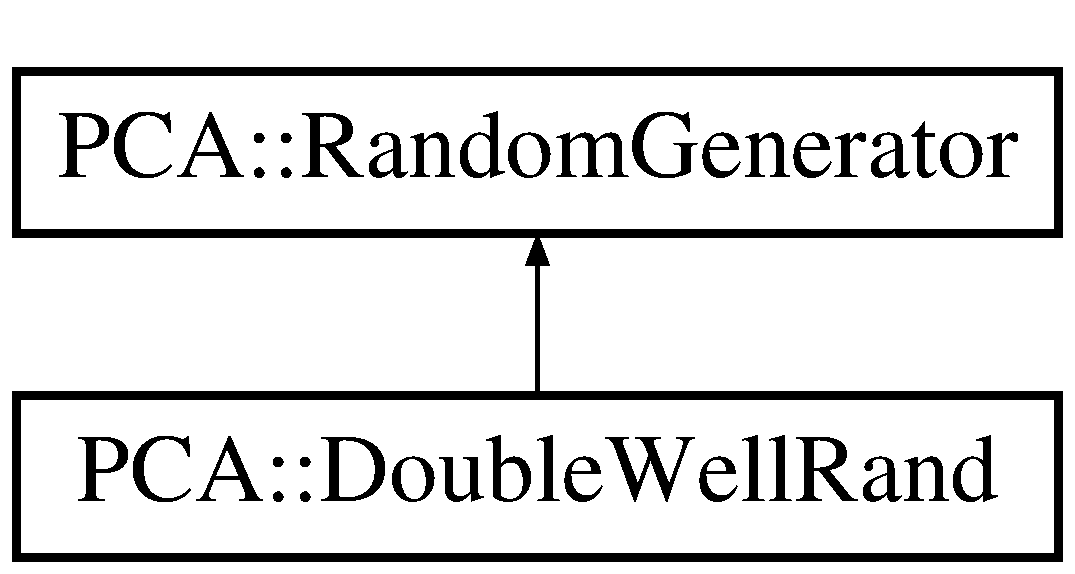
\includegraphics[height=2.000000cm]{class_p_c_a_1_1_double_well_rand}
\end{center}
\end{figure}
\subsection*{Public Member Functions}
\begin{DoxyCompactItemize}
\item 
\hyperlink{class_p_c_a_1_1_double_well_rand_a5a804723b5487331965c41acfaed8f0a}{Double\+Well\+Rand} (double a\+\_\+in, double b\+\_\+in, double c\+\_\+in, double offset\+\_\+in=10.\+0)
\item 
\hyperlink{class_p_c_a_1_1_double_well_rand_aafd6d9bf8587eda1cb46e45686cf772a}{$\sim$\+Double\+Well\+Rand} ()
\item 
virtual double \hyperlink{class_p_c_a_1_1_double_well_rand_a13beb4ae56cd6ccb1d6e4c1e2a03ff9b}{operator()} ()
\begin{DoxyCompactList}\small\item\em overloading operator () \end{DoxyCompactList}\item 
void \hyperlink{class_p_c_a_1_1_double_well_rand_aead9619d86b833eb5d9753a94294bc93}{write\+Log\+File} (F\+I\+LE $\ast$log\+\_\+file) const
\begin{DoxyCompactList}\small\item\em parameters output \end{DoxyCompactList}\end{DoxyCompactItemize}
\subsection*{Private Member Functions}
\begin{DoxyCompactItemize}
\item 
double \hyperlink{class_p_c_a_1_1_double_well_rand_a345fbcb1a01172464184b418ee761442}{polynom} (double x) const
\item 
double \hyperlink{class_p_c_a_1_1_double_well_rand_ab3817725d51a9171ef6a7e6a72ce25ef}{first\+Derivative} (double x) const
\item 
double \hyperlink{class_p_c_a_1_1_double_well_rand_a20c4fa6e77dad5161a214706adeda281}{second\+Derivative} (double x) const
\item 
void \hyperlink{class_p_c_a_1_1_double_well_rand_aa798efa59786f8aeeafb198f4a3319a3}{find\+Maxima} ()
\item 
void \hyperlink{class_p_c_a_1_1_double_well_rand_a89905058cce9c8bbecd5a0dabd21ea3c}{find\+Intervals} ()
\item 
void \hyperlink{class_p_c_a_1_1_double_well_rand_ab4d8dfc2a37b647e55fd18cc1d8e11f9}{find\+Norm\+Coefficients} ()
\item 
void \hyperlink{class_p_c_a_1_1_double_well_rand_a60ad7eeeb8f90a0e7312689820591674}{sort\+\_\+asc} ()
\end{DoxyCompactItemize}
\subsection*{Private Attributes}
\begin{DoxyCompactItemize}
\item 
\hyperlink{class_p_c_a_1_1_uniform_rand}{Uniform\+Rand} \hyperlink{class_p_c_a_1_1_double_well_rand_a44577274c594e30092748eb446d8dd40}{uni\+Rand}
\begin{DoxyCompactList}\small\item\em random number generator; \end{DoxyCompactList}\item 
double \hyperlink{class_p_c_a_1_1_double_well_rand_abad044e066c9b93b3eacb6d36440f650}{offset}
\begin{DoxyCompactList}\small\item\em offset from maximal value of polynom; \end{DoxyCompactList}\item 
int \hyperlink{class_p_c_a_1_1_double_well_rand_a89c48e652127b71600906d93f628dad5}{n\+\_\+intervals}
\begin{DoxyCompactList}\small\item\em number of intervals (1 or 2) \end{DoxyCompactList}\item 
double \hyperlink{class_p_c_a_1_1_double_well_rand_a4792680466fc8f865be362937b3e4e3b}{kappa} \mbox{[}4\mbox{]}
\begin{DoxyCompactList}\small\item\em borders of working intervals (kappa\mbox{[}0\mbox{]} and kappa\mbox{[}1\mbox{]} -\/ 1st interval, kappa\mbox{[}2\mbox{]} and kappa\mbox{[}3\mbox{]} -\/ 2d interval(if existd)) \end{DoxyCompactList}\item 
double \hyperlink{class_p_c_a_1_1_double_well_rand_a5fa2e0c609851d3e8a8cb9eb4bbd90c6}{im\+\_\+epsilon} = 1e-\/5
\begin{DoxyCompactList}\small\item\em tolerance to imaginary part of the polynom roots \end{DoxyCompactList}\item 
double \hyperlink{class_p_c_a_1_1_double_well_rand_aa31900946aeacdd5f462704393b93413}{norm} \mbox{[}2\mbox{]}
\begin{DoxyCompactList}\small\item\em normalizing coefficients in each interval (if one interval -\/ only norm\mbox{[}0\mbox{]} is used) \end{DoxyCompactList}\item 
int \hyperlink{class_p_c_a_1_1_double_well_rand_a935058a518ed28d62b9e2285c30382dc}{N\+\_\+int\+\_\+steps} = 50
\begin{DoxyCompactList}\small\item\em number of steps during integration \end{DoxyCompactList}\item 
int \hyperlink{class_p_c_a_1_1_double_well_rand_ab5eed0e97bd8309d5fa44fa2c7d8cbfd}{error\+\_\+code}
\begin{DoxyCompactList}\small\item\em 0 if everything is ok; \end{DoxyCompactList}\end{DoxyCompactItemize}
\begin{Indent}{\bf Parameters of the distribution\+:}\par
\begin{DoxyCompactItemize}
\item 
double \hyperlink{class_p_c_a_1_1_double_well_rand_a2291611a2ea4d9c3ee50a904c2fea9b7}{a}
\item 
double \hyperlink{class_p_c_a_1_1_double_well_rand_a289b59fbd571f8f377888f48a8c6b8ae}{b}
\item 
double \hyperlink{class_p_c_a_1_1_double_well_rand_a855b2106b6b692f9e837ef282b658c85}{c}
\end{DoxyCompactItemize}
\end{Indent}
\begin{Indent}{\bf Roots of the first derivative\+:}\par
\begin{DoxyCompactItemize}
\item 
double \hyperlink{class_p_c_a_1_1_double_well_rand_ab624775bcfb6b575ae1aa099bcd78cd7}{x1}
\item 
double \hyperlink{class_p_c_a_1_1_double_well_rand_a116879814f1ddd7bfc1efc3c11bf8c5b}{x2}
\item 
double \hyperlink{class_p_c_a_1_1_double_well_rand_a2ac7d1cea509a918639ccb8bef3f1d0a}{x3}
\end{DoxyCompactItemize}
\end{Indent}
\begin{Indent}{\bf Maxima\+:}\par
\begin{DoxyCompactItemize}
\item 
int \hyperlink{class_p_c_a_1_1_double_well_rand_ae53977982288d0b187a7fab536bbc55b}{n\+\_\+maxima}
\begin{DoxyCompactList}\small\item\em number of maxima (2 or 4) \end{DoxyCompactList}\item 
double \hyperlink{class_p_c_a_1_1_double_well_rand_a69b543f7eb8dda81f522a2002af65456}{x\+\_\+max1}
\begin{DoxyCompactList}\small\item\em argument of global maximum \end{DoxyCompactList}\item 
double \hyperlink{class_p_c_a_1_1_double_well_rand_a2fd3ef155f258ef1393fdb5ae503e2b0}{x\+\_\+max2}
\begin{DoxyCompactList}\small\item\em N\+U\+LL if there is only one maximum. \end{DoxyCompactList}\item 
double \hyperlink{class_p_c_a_1_1_double_well_rand_a627173c860baf5c9744916fc9e203404}{f\+\_\+max1}
\begin{DoxyCompactList}\small\item\em global maximum \end{DoxyCompactList}\item 
double \hyperlink{class_p_c_a_1_1_double_well_rand_a05278693e04d00a31bd41dedb38926b7}{f\+\_\+max2}
\begin{DoxyCompactList}\small\item\em N\+U\+LL if there is only one maximum. \end{DoxyCompactList}\end{DoxyCompactItemize}
\end{Indent}
\subsection*{Additional Inherited Members}


\subsection{Detailed Description}
Generate random numbers according distribution\+: \[ P = \exp(-ax^4+bx^2+cx) \] for \[ a>0 \]. 

\subsection{Constructor \& Destructor Documentation}
\hypertarget{class_p_c_a_1_1_double_well_rand_a5a804723b5487331965c41acfaed8f0a}{}\label{class_p_c_a_1_1_double_well_rand_a5a804723b5487331965c41acfaed8f0a} 
\index{P\+C\+A\+::\+Double\+Well\+Rand@{P\+C\+A\+::\+Double\+Well\+Rand}!Double\+Well\+Rand@{Double\+Well\+Rand}}
\index{Double\+Well\+Rand@{Double\+Well\+Rand}!P\+C\+A\+::\+Double\+Well\+Rand@{P\+C\+A\+::\+Double\+Well\+Rand}}
\subsubsection{\texorpdfstring{Double\+Well\+Rand()}{DoubleWellRand()}}
{\footnotesize\ttfamily P\+C\+A\+::\+Double\+Well\+Rand\+::\+Double\+Well\+Rand (\begin{DoxyParamCaption}\item[{double}]{a\+\_\+in,  }\item[{double}]{b\+\_\+in,  }\item[{double}]{c\+\_\+in,  }\item[{double}]{offset\+\_\+in = {\ttfamily 10.0} }\end{DoxyParamCaption})}

\hypertarget{class_p_c_a_1_1_double_well_rand_aafd6d9bf8587eda1cb46e45686cf772a}{}\label{class_p_c_a_1_1_double_well_rand_aafd6d9bf8587eda1cb46e45686cf772a} 
\index{P\+C\+A\+::\+Double\+Well\+Rand@{P\+C\+A\+::\+Double\+Well\+Rand}!````~Double\+Well\+Rand@{$\sim$\+Double\+Well\+Rand}}
\index{````~Double\+Well\+Rand@{$\sim$\+Double\+Well\+Rand}!P\+C\+A\+::\+Double\+Well\+Rand@{P\+C\+A\+::\+Double\+Well\+Rand}}
\subsubsection{\texorpdfstring{$\sim$\+Double\+Well\+Rand()}{~DoubleWellRand()}}
{\footnotesize\ttfamily P\+C\+A\+::\+Double\+Well\+Rand\+::$\sim$\+Double\+Well\+Rand (\begin{DoxyParamCaption}{ }\end{DoxyParamCaption})}



\subsection{Member Function Documentation}
\hypertarget{class_p_c_a_1_1_double_well_rand_a89905058cce9c8bbecd5a0dabd21ea3c}{}\label{class_p_c_a_1_1_double_well_rand_a89905058cce9c8bbecd5a0dabd21ea3c} 
\index{P\+C\+A\+::\+Double\+Well\+Rand@{P\+C\+A\+::\+Double\+Well\+Rand}!find\+Intervals@{find\+Intervals}}
\index{find\+Intervals@{find\+Intervals}!P\+C\+A\+::\+Double\+Well\+Rand@{P\+C\+A\+::\+Double\+Well\+Rand}}
\subsubsection{\texorpdfstring{find\+Intervals()}{findIntervals()}}
{\footnotesize\ttfamily void P\+C\+A\+::\+Double\+Well\+Rand\+::find\+Intervals (\begin{DoxyParamCaption}{ }\end{DoxyParamCaption})\hspace{0.3cm}{\ttfamily [private]}}

\hypertarget{class_p_c_a_1_1_double_well_rand_aa798efa59786f8aeeafb198f4a3319a3}{}\label{class_p_c_a_1_1_double_well_rand_aa798efa59786f8aeeafb198f4a3319a3} 
\index{P\+C\+A\+::\+Double\+Well\+Rand@{P\+C\+A\+::\+Double\+Well\+Rand}!find\+Maxima@{find\+Maxima}}
\index{find\+Maxima@{find\+Maxima}!P\+C\+A\+::\+Double\+Well\+Rand@{P\+C\+A\+::\+Double\+Well\+Rand}}
\subsubsection{\texorpdfstring{find\+Maxima()}{findMaxima()}}
{\footnotesize\ttfamily void P\+C\+A\+::\+Double\+Well\+Rand\+::find\+Maxima (\begin{DoxyParamCaption}{ }\end{DoxyParamCaption})\hspace{0.3cm}{\ttfamily [private]}}

\hypertarget{class_p_c_a_1_1_double_well_rand_ab4d8dfc2a37b647e55fd18cc1d8e11f9}{}\label{class_p_c_a_1_1_double_well_rand_ab4d8dfc2a37b647e55fd18cc1d8e11f9} 
\index{P\+C\+A\+::\+Double\+Well\+Rand@{P\+C\+A\+::\+Double\+Well\+Rand}!find\+Norm\+Coefficients@{find\+Norm\+Coefficients}}
\index{find\+Norm\+Coefficients@{find\+Norm\+Coefficients}!P\+C\+A\+::\+Double\+Well\+Rand@{P\+C\+A\+::\+Double\+Well\+Rand}}
\subsubsection{\texorpdfstring{find\+Norm\+Coefficients()}{findNormCoefficients()}}
{\footnotesize\ttfamily void P\+C\+A\+::\+Double\+Well\+Rand\+::find\+Norm\+Coefficients (\begin{DoxyParamCaption}{ }\end{DoxyParamCaption})\hspace{0.3cm}{\ttfamily [private]}}

\hypertarget{class_p_c_a_1_1_double_well_rand_ab3817725d51a9171ef6a7e6a72ce25ef}{}\label{class_p_c_a_1_1_double_well_rand_ab3817725d51a9171ef6a7e6a72ce25ef} 
\index{P\+C\+A\+::\+Double\+Well\+Rand@{P\+C\+A\+::\+Double\+Well\+Rand}!first\+Derivative@{first\+Derivative}}
\index{first\+Derivative@{first\+Derivative}!P\+C\+A\+::\+Double\+Well\+Rand@{P\+C\+A\+::\+Double\+Well\+Rand}}
\subsubsection{\texorpdfstring{first\+Derivative()}{firstDerivative()}}
{\footnotesize\ttfamily double P\+C\+A\+::\+Double\+Well\+Rand\+::first\+Derivative (\begin{DoxyParamCaption}\item[{double}]{x }\end{DoxyParamCaption}) const\hspace{0.3cm}{\ttfamily [private]}}

\hypertarget{class_p_c_a_1_1_double_well_rand_a13beb4ae56cd6ccb1d6e4c1e2a03ff9b}{}\label{class_p_c_a_1_1_double_well_rand_a13beb4ae56cd6ccb1d6e4c1e2a03ff9b} 
\index{P\+C\+A\+::\+Double\+Well\+Rand@{P\+C\+A\+::\+Double\+Well\+Rand}!operator()@{operator()}}
\index{operator()@{operator()}!P\+C\+A\+::\+Double\+Well\+Rand@{P\+C\+A\+::\+Double\+Well\+Rand}}
\subsubsection{\texorpdfstring{operator()()}{operator()()}}
{\footnotesize\ttfamily double P\+C\+A\+::\+Double\+Well\+Rand\+::operator() (\begin{DoxyParamCaption}{ }\end{DoxyParamCaption})\hspace{0.3cm}{\ttfamily [virtual]}}



overloading operator () 



Implements \hyperlink{class_p_c_a_1_1_random_generator_a4361e39397900ae1e7b2cfa91a592509}{P\+C\+A\+::\+Random\+Generator}.

\hypertarget{class_p_c_a_1_1_double_well_rand_a345fbcb1a01172464184b418ee761442}{}\label{class_p_c_a_1_1_double_well_rand_a345fbcb1a01172464184b418ee761442} 
\index{P\+C\+A\+::\+Double\+Well\+Rand@{P\+C\+A\+::\+Double\+Well\+Rand}!polynom@{polynom}}
\index{polynom@{polynom}!P\+C\+A\+::\+Double\+Well\+Rand@{P\+C\+A\+::\+Double\+Well\+Rand}}
\subsubsection{\texorpdfstring{polynom()}{polynom()}}
{\footnotesize\ttfamily double P\+C\+A\+::\+Double\+Well\+Rand\+::polynom (\begin{DoxyParamCaption}\item[{double}]{x }\end{DoxyParamCaption}) const\hspace{0.3cm}{\ttfamily [private]}}

\hypertarget{class_p_c_a_1_1_double_well_rand_a20c4fa6e77dad5161a214706adeda281}{}\label{class_p_c_a_1_1_double_well_rand_a20c4fa6e77dad5161a214706adeda281} 
\index{P\+C\+A\+::\+Double\+Well\+Rand@{P\+C\+A\+::\+Double\+Well\+Rand}!second\+Derivative@{second\+Derivative}}
\index{second\+Derivative@{second\+Derivative}!P\+C\+A\+::\+Double\+Well\+Rand@{P\+C\+A\+::\+Double\+Well\+Rand}}
\subsubsection{\texorpdfstring{second\+Derivative()}{secondDerivative()}}
{\footnotesize\ttfamily double P\+C\+A\+::\+Double\+Well\+Rand\+::second\+Derivative (\begin{DoxyParamCaption}\item[{double}]{x }\end{DoxyParamCaption}) const\hspace{0.3cm}{\ttfamily [private]}}

\hypertarget{class_p_c_a_1_1_double_well_rand_a60ad7eeeb8f90a0e7312689820591674}{}\label{class_p_c_a_1_1_double_well_rand_a60ad7eeeb8f90a0e7312689820591674} 
\index{P\+C\+A\+::\+Double\+Well\+Rand@{P\+C\+A\+::\+Double\+Well\+Rand}!sort\+\_\+asc@{sort\+\_\+asc}}
\index{sort\+\_\+asc@{sort\+\_\+asc}!P\+C\+A\+::\+Double\+Well\+Rand@{P\+C\+A\+::\+Double\+Well\+Rand}}
\subsubsection{\texorpdfstring{sort\+\_\+asc()}{sort\_asc()}}
{\footnotesize\ttfamily void P\+C\+A\+::\+Double\+Well\+Rand\+::sort\+\_\+asc (\begin{DoxyParamCaption}{ }\end{DoxyParamCaption})\hspace{0.3cm}{\ttfamily [private]}}

\hypertarget{class_p_c_a_1_1_double_well_rand_aead9619d86b833eb5d9753a94294bc93}{}\label{class_p_c_a_1_1_double_well_rand_aead9619d86b833eb5d9753a94294bc93} 
\index{P\+C\+A\+::\+Double\+Well\+Rand@{P\+C\+A\+::\+Double\+Well\+Rand}!write\+Log\+File@{write\+Log\+File}}
\index{write\+Log\+File@{write\+Log\+File}!P\+C\+A\+::\+Double\+Well\+Rand@{P\+C\+A\+::\+Double\+Well\+Rand}}
\subsubsection{\texorpdfstring{write\+Log\+File()}{writeLogFile()}}
{\footnotesize\ttfamily void P\+C\+A\+::\+Double\+Well\+Rand\+::write\+Log\+File (\begin{DoxyParamCaption}\item[{F\+I\+LE $\ast$}]{log\+\_\+file }\end{DoxyParamCaption}) const}



parameters output 



\subsection{Member Data Documentation}
\hypertarget{class_p_c_a_1_1_double_well_rand_a2291611a2ea4d9c3ee50a904c2fea9b7}{}\label{class_p_c_a_1_1_double_well_rand_a2291611a2ea4d9c3ee50a904c2fea9b7} 
\index{P\+C\+A\+::\+Double\+Well\+Rand@{P\+C\+A\+::\+Double\+Well\+Rand}!a@{a}}
\index{a@{a}!P\+C\+A\+::\+Double\+Well\+Rand@{P\+C\+A\+::\+Double\+Well\+Rand}}
\subsubsection{\texorpdfstring{a}{a}}
{\footnotesize\ttfamily double P\+C\+A\+::\+Double\+Well\+Rand\+::a\hspace{0.3cm}{\ttfamily [private]}}

\hypertarget{class_p_c_a_1_1_double_well_rand_a289b59fbd571f8f377888f48a8c6b8ae}{}\label{class_p_c_a_1_1_double_well_rand_a289b59fbd571f8f377888f48a8c6b8ae} 
\index{P\+C\+A\+::\+Double\+Well\+Rand@{P\+C\+A\+::\+Double\+Well\+Rand}!b@{b}}
\index{b@{b}!P\+C\+A\+::\+Double\+Well\+Rand@{P\+C\+A\+::\+Double\+Well\+Rand}}
\subsubsection{\texorpdfstring{b}{b}}
{\footnotesize\ttfamily double P\+C\+A\+::\+Double\+Well\+Rand\+::b\hspace{0.3cm}{\ttfamily [private]}}

\hypertarget{class_p_c_a_1_1_double_well_rand_a855b2106b6b692f9e837ef282b658c85}{}\label{class_p_c_a_1_1_double_well_rand_a855b2106b6b692f9e837ef282b658c85} 
\index{P\+C\+A\+::\+Double\+Well\+Rand@{P\+C\+A\+::\+Double\+Well\+Rand}!c@{c}}
\index{c@{c}!P\+C\+A\+::\+Double\+Well\+Rand@{P\+C\+A\+::\+Double\+Well\+Rand}}
\subsubsection{\texorpdfstring{c}{c}}
{\footnotesize\ttfamily double P\+C\+A\+::\+Double\+Well\+Rand\+::c\hspace{0.3cm}{\ttfamily [private]}}

\hypertarget{class_p_c_a_1_1_double_well_rand_ab5eed0e97bd8309d5fa44fa2c7d8cbfd}{}\label{class_p_c_a_1_1_double_well_rand_ab5eed0e97bd8309d5fa44fa2c7d8cbfd} 
\index{P\+C\+A\+::\+Double\+Well\+Rand@{P\+C\+A\+::\+Double\+Well\+Rand}!error\+\_\+code@{error\+\_\+code}}
\index{error\+\_\+code@{error\+\_\+code}!P\+C\+A\+::\+Double\+Well\+Rand@{P\+C\+A\+::\+Double\+Well\+Rand}}
\subsubsection{\texorpdfstring{error\+\_\+code}{error\_code}}
{\footnotesize\ttfamily int P\+C\+A\+::\+Double\+Well\+Rand\+::error\+\_\+code\hspace{0.3cm}{\ttfamily [private]}}



0 if everything is ok; 

\hypertarget{class_p_c_a_1_1_double_well_rand_a627173c860baf5c9744916fc9e203404}{}\label{class_p_c_a_1_1_double_well_rand_a627173c860baf5c9744916fc9e203404} 
\index{P\+C\+A\+::\+Double\+Well\+Rand@{P\+C\+A\+::\+Double\+Well\+Rand}!f\+\_\+max1@{f\+\_\+max1}}
\index{f\+\_\+max1@{f\+\_\+max1}!P\+C\+A\+::\+Double\+Well\+Rand@{P\+C\+A\+::\+Double\+Well\+Rand}}
\subsubsection{\texorpdfstring{f\+\_\+max1}{f\_max1}}
{\footnotesize\ttfamily double P\+C\+A\+::\+Double\+Well\+Rand\+::f\+\_\+max1\hspace{0.3cm}{\ttfamily [private]}}



global maximum 

\hypertarget{class_p_c_a_1_1_double_well_rand_a05278693e04d00a31bd41dedb38926b7}{}\label{class_p_c_a_1_1_double_well_rand_a05278693e04d00a31bd41dedb38926b7} 
\index{P\+C\+A\+::\+Double\+Well\+Rand@{P\+C\+A\+::\+Double\+Well\+Rand}!f\+\_\+max2@{f\+\_\+max2}}
\index{f\+\_\+max2@{f\+\_\+max2}!P\+C\+A\+::\+Double\+Well\+Rand@{P\+C\+A\+::\+Double\+Well\+Rand}}
\subsubsection{\texorpdfstring{f\+\_\+max2}{f\_max2}}
{\footnotesize\ttfamily double P\+C\+A\+::\+Double\+Well\+Rand\+::f\+\_\+max2\hspace{0.3cm}{\ttfamily [private]}}



N\+U\+LL if there is only one maximum. 

\hypertarget{class_p_c_a_1_1_double_well_rand_a5fa2e0c609851d3e8a8cb9eb4bbd90c6}{}\label{class_p_c_a_1_1_double_well_rand_a5fa2e0c609851d3e8a8cb9eb4bbd90c6} 
\index{P\+C\+A\+::\+Double\+Well\+Rand@{P\+C\+A\+::\+Double\+Well\+Rand}!im\+\_\+epsilon@{im\+\_\+epsilon}}
\index{im\+\_\+epsilon@{im\+\_\+epsilon}!P\+C\+A\+::\+Double\+Well\+Rand@{P\+C\+A\+::\+Double\+Well\+Rand}}
\subsubsection{\texorpdfstring{im\+\_\+epsilon}{im\_epsilon}}
{\footnotesize\ttfamily double P\+C\+A\+::\+Double\+Well\+Rand\+::im\+\_\+epsilon = 1e-\/5\hspace{0.3cm}{\ttfamily [private]}}



tolerance to imaginary part of the polynom roots 

\hypertarget{class_p_c_a_1_1_double_well_rand_a4792680466fc8f865be362937b3e4e3b}{}\label{class_p_c_a_1_1_double_well_rand_a4792680466fc8f865be362937b3e4e3b} 
\index{P\+C\+A\+::\+Double\+Well\+Rand@{P\+C\+A\+::\+Double\+Well\+Rand}!kappa@{kappa}}
\index{kappa@{kappa}!P\+C\+A\+::\+Double\+Well\+Rand@{P\+C\+A\+::\+Double\+Well\+Rand}}
\subsubsection{\texorpdfstring{kappa}{kappa}}
{\footnotesize\ttfamily double P\+C\+A\+::\+Double\+Well\+Rand\+::kappa\mbox{[}4\mbox{]}\hspace{0.3cm}{\ttfamily [private]}}



borders of working intervals (kappa\mbox{[}0\mbox{]} and kappa\mbox{[}1\mbox{]} -\/ 1st interval, kappa\mbox{[}2\mbox{]} and kappa\mbox{[}3\mbox{]} -\/ 2d interval(if existd)) 

\hypertarget{class_p_c_a_1_1_double_well_rand_a935058a518ed28d62b9e2285c30382dc}{}\label{class_p_c_a_1_1_double_well_rand_a935058a518ed28d62b9e2285c30382dc} 
\index{P\+C\+A\+::\+Double\+Well\+Rand@{P\+C\+A\+::\+Double\+Well\+Rand}!N\+\_\+int\+\_\+steps@{N\+\_\+int\+\_\+steps}}
\index{N\+\_\+int\+\_\+steps@{N\+\_\+int\+\_\+steps}!P\+C\+A\+::\+Double\+Well\+Rand@{P\+C\+A\+::\+Double\+Well\+Rand}}
\subsubsection{\texorpdfstring{N\+\_\+int\+\_\+steps}{N\_int\_steps}}
{\footnotesize\ttfamily int P\+C\+A\+::\+Double\+Well\+Rand\+::\+N\+\_\+int\+\_\+steps = 50\hspace{0.3cm}{\ttfamily [private]}}



number of steps during integration 

\hypertarget{class_p_c_a_1_1_double_well_rand_a89c48e652127b71600906d93f628dad5}{}\label{class_p_c_a_1_1_double_well_rand_a89c48e652127b71600906d93f628dad5} 
\index{P\+C\+A\+::\+Double\+Well\+Rand@{P\+C\+A\+::\+Double\+Well\+Rand}!n\+\_\+intervals@{n\+\_\+intervals}}
\index{n\+\_\+intervals@{n\+\_\+intervals}!P\+C\+A\+::\+Double\+Well\+Rand@{P\+C\+A\+::\+Double\+Well\+Rand}}
\subsubsection{\texorpdfstring{n\+\_\+intervals}{n\_intervals}}
{\footnotesize\ttfamily int P\+C\+A\+::\+Double\+Well\+Rand\+::n\+\_\+intervals\hspace{0.3cm}{\ttfamily [private]}}



number of intervals (1 or 2) 

\hypertarget{class_p_c_a_1_1_double_well_rand_ae53977982288d0b187a7fab536bbc55b}{}\label{class_p_c_a_1_1_double_well_rand_ae53977982288d0b187a7fab536bbc55b} 
\index{P\+C\+A\+::\+Double\+Well\+Rand@{P\+C\+A\+::\+Double\+Well\+Rand}!n\+\_\+maxima@{n\+\_\+maxima}}
\index{n\+\_\+maxima@{n\+\_\+maxima}!P\+C\+A\+::\+Double\+Well\+Rand@{P\+C\+A\+::\+Double\+Well\+Rand}}
\subsubsection{\texorpdfstring{n\+\_\+maxima}{n\_maxima}}
{\footnotesize\ttfamily int P\+C\+A\+::\+Double\+Well\+Rand\+::n\+\_\+maxima\hspace{0.3cm}{\ttfamily [private]}}



number of maxima (2 or 4) 

\hypertarget{class_p_c_a_1_1_double_well_rand_aa31900946aeacdd5f462704393b93413}{}\label{class_p_c_a_1_1_double_well_rand_aa31900946aeacdd5f462704393b93413} 
\index{P\+C\+A\+::\+Double\+Well\+Rand@{P\+C\+A\+::\+Double\+Well\+Rand}!norm@{norm}}
\index{norm@{norm}!P\+C\+A\+::\+Double\+Well\+Rand@{P\+C\+A\+::\+Double\+Well\+Rand}}
\subsubsection{\texorpdfstring{norm}{norm}}
{\footnotesize\ttfamily double P\+C\+A\+::\+Double\+Well\+Rand\+::norm\mbox{[}2\mbox{]}\hspace{0.3cm}{\ttfamily [private]}}



normalizing coefficients in each interval (if one interval -\/ only norm\mbox{[}0\mbox{]} is used) 

\hypertarget{class_p_c_a_1_1_double_well_rand_abad044e066c9b93b3eacb6d36440f650}{}\label{class_p_c_a_1_1_double_well_rand_abad044e066c9b93b3eacb6d36440f650} 
\index{P\+C\+A\+::\+Double\+Well\+Rand@{P\+C\+A\+::\+Double\+Well\+Rand}!offset@{offset}}
\index{offset@{offset}!P\+C\+A\+::\+Double\+Well\+Rand@{P\+C\+A\+::\+Double\+Well\+Rand}}
\subsubsection{\texorpdfstring{offset}{offset}}
{\footnotesize\ttfamily double P\+C\+A\+::\+Double\+Well\+Rand\+::offset\hspace{0.3cm}{\ttfamily [private]}}



offset from maximal value of polynom; 

\hypertarget{class_p_c_a_1_1_double_well_rand_a44577274c594e30092748eb446d8dd40}{}\label{class_p_c_a_1_1_double_well_rand_a44577274c594e30092748eb446d8dd40} 
\index{P\+C\+A\+::\+Double\+Well\+Rand@{P\+C\+A\+::\+Double\+Well\+Rand}!uni\+Rand@{uni\+Rand}}
\index{uni\+Rand@{uni\+Rand}!P\+C\+A\+::\+Double\+Well\+Rand@{P\+C\+A\+::\+Double\+Well\+Rand}}
\subsubsection{\texorpdfstring{uni\+Rand}{uniRand}}
{\footnotesize\ttfamily \hyperlink{class_p_c_a_1_1_uniform_rand}{Uniform\+Rand} P\+C\+A\+::\+Double\+Well\+Rand\+::uni\+Rand\hspace{0.3cm}{\ttfamily [private]}}



random number generator; 

\hypertarget{class_p_c_a_1_1_double_well_rand_ab624775bcfb6b575ae1aa099bcd78cd7}{}\label{class_p_c_a_1_1_double_well_rand_ab624775bcfb6b575ae1aa099bcd78cd7} 
\index{P\+C\+A\+::\+Double\+Well\+Rand@{P\+C\+A\+::\+Double\+Well\+Rand}!x1@{x1}}
\index{x1@{x1}!P\+C\+A\+::\+Double\+Well\+Rand@{P\+C\+A\+::\+Double\+Well\+Rand}}
\subsubsection{\texorpdfstring{x1}{x1}}
{\footnotesize\ttfamily double P\+C\+A\+::\+Double\+Well\+Rand\+::x1\hspace{0.3cm}{\ttfamily [private]}}

\hypertarget{class_p_c_a_1_1_double_well_rand_a116879814f1ddd7bfc1efc3c11bf8c5b}{}\label{class_p_c_a_1_1_double_well_rand_a116879814f1ddd7bfc1efc3c11bf8c5b} 
\index{P\+C\+A\+::\+Double\+Well\+Rand@{P\+C\+A\+::\+Double\+Well\+Rand}!x2@{x2}}
\index{x2@{x2}!P\+C\+A\+::\+Double\+Well\+Rand@{P\+C\+A\+::\+Double\+Well\+Rand}}
\subsubsection{\texorpdfstring{x2}{x2}}
{\footnotesize\ttfamily double P\+C\+A\+::\+Double\+Well\+Rand\+::x2\hspace{0.3cm}{\ttfamily [private]}}

\hypertarget{class_p_c_a_1_1_double_well_rand_a2ac7d1cea509a918639ccb8bef3f1d0a}{}\label{class_p_c_a_1_1_double_well_rand_a2ac7d1cea509a918639ccb8bef3f1d0a} 
\index{P\+C\+A\+::\+Double\+Well\+Rand@{P\+C\+A\+::\+Double\+Well\+Rand}!x3@{x3}}
\index{x3@{x3}!P\+C\+A\+::\+Double\+Well\+Rand@{P\+C\+A\+::\+Double\+Well\+Rand}}
\subsubsection{\texorpdfstring{x3}{x3}}
{\footnotesize\ttfamily double P\+C\+A\+::\+Double\+Well\+Rand\+::x3\hspace{0.3cm}{\ttfamily [private]}}

\hypertarget{class_p_c_a_1_1_double_well_rand_a69b543f7eb8dda81f522a2002af65456}{}\label{class_p_c_a_1_1_double_well_rand_a69b543f7eb8dda81f522a2002af65456} 
\index{P\+C\+A\+::\+Double\+Well\+Rand@{P\+C\+A\+::\+Double\+Well\+Rand}!x\+\_\+max1@{x\+\_\+max1}}
\index{x\+\_\+max1@{x\+\_\+max1}!P\+C\+A\+::\+Double\+Well\+Rand@{P\+C\+A\+::\+Double\+Well\+Rand}}
\subsubsection{\texorpdfstring{x\+\_\+max1}{x\_max1}}
{\footnotesize\ttfamily double P\+C\+A\+::\+Double\+Well\+Rand\+::x\+\_\+max1\hspace{0.3cm}{\ttfamily [private]}}



argument of global maximum 

\hypertarget{class_p_c_a_1_1_double_well_rand_a2fd3ef155f258ef1393fdb5ae503e2b0}{}\label{class_p_c_a_1_1_double_well_rand_a2fd3ef155f258ef1393fdb5ae503e2b0} 
\index{P\+C\+A\+::\+Double\+Well\+Rand@{P\+C\+A\+::\+Double\+Well\+Rand}!x\+\_\+max2@{x\+\_\+max2}}
\index{x\+\_\+max2@{x\+\_\+max2}!P\+C\+A\+::\+Double\+Well\+Rand@{P\+C\+A\+::\+Double\+Well\+Rand}}
\subsubsection{\texorpdfstring{x\+\_\+max2}{x\_max2}}
{\footnotesize\ttfamily double P\+C\+A\+::\+Double\+Well\+Rand\+::x\+\_\+max2\hspace{0.3cm}{\ttfamily [private]}}



N\+U\+LL if there is only one maximum. 



The documentation for this class was generated from the following files\+:\begin{DoxyCompactItemize}
\item 
/\+Users/annsi118/\+Documents/\+Git\+\_\+projects/\+P\+C\+M\+C/include/\+Random/\hyperlink{_double_well_rand_8h}{Double\+Well\+Rand.\+h}\item 
/\+Users/annsi118/\+Documents/\+Git\+\_\+projects/\+P\+C\+M\+C/source/\+Random/\hyperlink{_double_well_rand_8cpp}{Double\+Well\+Rand.\+cpp}\end{DoxyCompactItemize}

\hypertarget{class_p_c_a_1_1_polymer_energy_1_1_d_wparam}{}\section{P\+CA\+:\+:Polymer\+Energy\+:\+:D\+Wparam Class Reference}
\label{class_p_c_a_1_1_polymer_energy_1_1_d_wparam}\index{P\+C\+A\+::\+Polymer\+Energy\+::\+D\+Wparam@{P\+C\+A\+::\+Polymer\+Energy\+::\+D\+Wparam}}


Parameters for double-\/well potential.  




{\ttfamily \#include $<$Polymer\+Energy.\+h$>$}

\subsection*{Public Member Functions}
\begin{DoxyCompactItemize}
\item 
\hyperlink{class_p_c_a_1_1_polymer_energy_1_1_d_wparam_a803a7fd6bcd83efd7934ad06a5fe6b71}{D\+Wparam} (int num\+Sites\+\_\+in, double q\+\_\+in, double m\+\_\+in, double c\+\_\+in, double d\+\_\+in, double a\+\_\+in, double b\+\_\+in=0, double u\+\_\+in=0)
\item 
\hyperlink{class_p_c_a_1_1_polymer_energy_1_1_d_wparam_af9a9a24e85422d933fb527ef43a620a0}{D\+Wparam} (int num\+Sites\+\_\+in, const double $\ast$q\+\_\+in, const double $\ast$m\+\_\+in, const double $\ast$c\+\_\+in, const double $\ast$d\+\_\+in, const double $\ast$a\+\_\+in, const double $\ast$b\+\_\+in=0, const double $\ast$u\+\_\+in=0)
\item 
\hyperlink{class_p_c_a_1_1_polymer_energy_1_1_d_wparam_a97b71972cd114d0a5a0aed004ec3a9f8}{$\sim$\+D\+Wparam} ()
\end{DoxyCompactItemize}
\subsection*{Public Attributes}
\begin{DoxyCompactItemize}
\item 
int \hyperlink{class_p_c_a_1_1_polymer_energy_1_1_d_wparam_abec5b658b4c55c10b6b98ced9db46d03}{num\+Sites}
\item 
double $\ast$ \hyperlink{class_p_c_a_1_1_polymer_energy_1_1_d_wparam_aa81ddf89c6aeaeb56aa453206937fea0}{q}
\item 
double $\ast$ \hyperlink{class_p_c_a_1_1_polymer_energy_1_1_d_wparam_a2c7311aadb8e50991e81a7a356bf272a}{m}
\item 
double $\ast$ \hyperlink{class_p_c_a_1_1_polymer_energy_1_1_d_wparam_aba580654697b1b865d245c76be7ecafb}{c}
\item 
double $\ast$ \hyperlink{class_p_c_a_1_1_polymer_energy_1_1_d_wparam_abb53ce45fe1085b443b6070afb080373}{d}
\item 
double $\ast$ \hyperlink{class_p_c_a_1_1_polymer_energy_1_1_d_wparam_a04564ebaeb5a082c0aea0b184aa84faf}{a}
\item 
double $\ast$ \hyperlink{class_p_c_a_1_1_polymer_energy_1_1_d_wparam_a956852f19d2c08dd73b5a5b392d79bae}{b}
\item 
double $\ast$ \hyperlink{class_p_c_a_1_1_polymer_energy_1_1_d_wparam_af0c288045dda1bafb7bdea671a0cdf2a}{u}
\end{DoxyCompactItemize}


\subsection{Detailed Description}
Parameters for double-\/well potential. 

\subsection{Constructor \& Destructor Documentation}
\hypertarget{class_p_c_a_1_1_polymer_energy_1_1_d_wparam_a803a7fd6bcd83efd7934ad06a5fe6b71}{}\label{class_p_c_a_1_1_polymer_energy_1_1_d_wparam_a803a7fd6bcd83efd7934ad06a5fe6b71} 
\index{P\+C\+A\+::\+Polymer\+Energy\+::\+D\+Wparam@{P\+C\+A\+::\+Polymer\+Energy\+::\+D\+Wparam}!D\+Wparam@{D\+Wparam}}
\index{D\+Wparam@{D\+Wparam}!P\+C\+A\+::\+Polymer\+Energy\+::\+D\+Wparam@{P\+C\+A\+::\+Polymer\+Energy\+::\+D\+Wparam}}
\subsubsection{\texorpdfstring{D\+Wparam()}{DWparam()}\hspace{0.1cm}{\footnotesize\ttfamily [1/2]}}
{\footnotesize\ttfamily P\+C\+A\+::\+Polymer\+Energy\+::\+D\+Wparam\+::\+D\+Wparam (\begin{DoxyParamCaption}\item[{int}]{num\+Sites\+\_\+in,  }\item[{double}]{q\+\_\+in,  }\item[{double}]{m\+\_\+in,  }\item[{double}]{c\+\_\+in,  }\item[{double}]{d\+\_\+in,  }\item[{double}]{a\+\_\+in,  }\item[{double}]{b\+\_\+in = {\ttfamily 0},  }\item[{double}]{u\+\_\+in = {\ttfamily 0} }\end{DoxyParamCaption})}

\hypertarget{class_p_c_a_1_1_polymer_energy_1_1_d_wparam_af9a9a24e85422d933fb527ef43a620a0}{}\label{class_p_c_a_1_1_polymer_energy_1_1_d_wparam_af9a9a24e85422d933fb527ef43a620a0} 
\index{P\+C\+A\+::\+Polymer\+Energy\+::\+D\+Wparam@{P\+C\+A\+::\+Polymer\+Energy\+::\+D\+Wparam}!D\+Wparam@{D\+Wparam}}
\index{D\+Wparam@{D\+Wparam}!P\+C\+A\+::\+Polymer\+Energy\+::\+D\+Wparam@{P\+C\+A\+::\+Polymer\+Energy\+::\+D\+Wparam}}
\subsubsection{\texorpdfstring{D\+Wparam()}{DWparam()}\hspace{0.1cm}{\footnotesize\ttfamily [2/2]}}
{\footnotesize\ttfamily P\+C\+A\+::\+Polymer\+Energy\+::\+D\+Wparam\+::\+D\+Wparam (\begin{DoxyParamCaption}\item[{int}]{num\+Sites\+\_\+in,  }\item[{const double $\ast$}]{q\+\_\+in,  }\item[{const double $\ast$}]{m\+\_\+in,  }\item[{const double $\ast$}]{c\+\_\+in,  }\item[{const double $\ast$}]{d\+\_\+in,  }\item[{const double $\ast$}]{a\+\_\+in,  }\item[{const double $\ast$}]{b\+\_\+in = {\ttfamily 0},  }\item[{const double $\ast$}]{u\+\_\+in = {\ttfamily 0} }\end{DoxyParamCaption})}

\hypertarget{class_p_c_a_1_1_polymer_energy_1_1_d_wparam_a97b71972cd114d0a5a0aed004ec3a9f8}{}\label{class_p_c_a_1_1_polymer_energy_1_1_d_wparam_a97b71972cd114d0a5a0aed004ec3a9f8} 
\index{P\+C\+A\+::\+Polymer\+Energy\+::\+D\+Wparam@{P\+C\+A\+::\+Polymer\+Energy\+::\+D\+Wparam}!````~D\+Wparam@{$\sim$\+D\+Wparam}}
\index{````~D\+Wparam@{$\sim$\+D\+Wparam}!P\+C\+A\+::\+Polymer\+Energy\+::\+D\+Wparam@{P\+C\+A\+::\+Polymer\+Energy\+::\+D\+Wparam}}
\subsubsection{\texorpdfstring{$\sim$\+D\+Wparam()}{~DWparam()}}
{\footnotesize\ttfamily P\+C\+A\+::\+Polymer\+Energy\+::\+D\+Wparam\+::$\sim$\+D\+Wparam (\begin{DoxyParamCaption}{ }\end{DoxyParamCaption})}



\subsection{Member Data Documentation}
\hypertarget{class_p_c_a_1_1_polymer_energy_1_1_d_wparam_a04564ebaeb5a082c0aea0b184aa84faf}{}\label{class_p_c_a_1_1_polymer_energy_1_1_d_wparam_a04564ebaeb5a082c0aea0b184aa84faf} 
\index{P\+C\+A\+::\+Polymer\+Energy\+::\+D\+Wparam@{P\+C\+A\+::\+Polymer\+Energy\+::\+D\+Wparam}!a@{a}}
\index{a@{a}!P\+C\+A\+::\+Polymer\+Energy\+::\+D\+Wparam@{P\+C\+A\+::\+Polymer\+Energy\+::\+D\+Wparam}}
\subsubsection{\texorpdfstring{a}{a}}
{\footnotesize\ttfamily double$\ast$ P\+C\+A\+::\+Polymer\+Energy\+::\+D\+Wparam\+::a}

\hypertarget{class_p_c_a_1_1_polymer_energy_1_1_d_wparam_a956852f19d2c08dd73b5a5b392d79bae}{}\label{class_p_c_a_1_1_polymer_energy_1_1_d_wparam_a956852f19d2c08dd73b5a5b392d79bae} 
\index{P\+C\+A\+::\+Polymer\+Energy\+::\+D\+Wparam@{P\+C\+A\+::\+Polymer\+Energy\+::\+D\+Wparam}!b@{b}}
\index{b@{b}!P\+C\+A\+::\+Polymer\+Energy\+::\+D\+Wparam@{P\+C\+A\+::\+Polymer\+Energy\+::\+D\+Wparam}}
\subsubsection{\texorpdfstring{b}{b}}
{\footnotesize\ttfamily double$\ast$ P\+C\+A\+::\+Polymer\+Energy\+::\+D\+Wparam\+::b}

\hypertarget{class_p_c_a_1_1_polymer_energy_1_1_d_wparam_aba580654697b1b865d245c76be7ecafb}{}\label{class_p_c_a_1_1_polymer_energy_1_1_d_wparam_aba580654697b1b865d245c76be7ecafb} 
\index{P\+C\+A\+::\+Polymer\+Energy\+::\+D\+Wparam@{P\+C\+A\+::\+Polymer\+Energy\+::\+D\+Wparam}!c@{c}}
\index{c@{c}!P\+C\+A\+::\+Polymer\+Energy\+::\+D\+Wparam@{P\+C\+A\+::\+Polymer\+Energy\+::\+D\+Wparam}}
\subsubsection{\texorpdfstring{c}{c}}
{\footnotesize\ttfamily double$\ast$ P\+C\+A\+::\+Polymer\+Energy\+::\+D\+Wparam\+::c}

\hypertarget{class_p_c_a_1_1_polymer_energy_1_1_d_wparam_abb53ce45fe1085b443b6070afb080373}{}\label{class_p_c_a_1_1_polymer_energy_1_1_d_wparam_abb53ce45fe1085b443b6070afb080373} 
\index{P\+C\+A\+::\+Polymer\+Energy\+::\+D\+Wparam@{P\+C\+A\+::\+Polymer\+Energy\+::\+D\+Wparam}!d@{d}}
\index{d@{d}!P\+C\+A\+::\+Polymer\+Energy\+::\+D\+Wparam@{P\+C\+A\+::\+Polymer\+Energy\+::\+D\+Wparam}}
\subsubsection{\texorpdfstring{d}{d}}
{\footnotesize\ttfamily double$\ast$ P\+C\+A\+::\+Polymer\+Energy\+::\+D\+Wparam\+::d}

\hypertarget{class_p_c_a_1_1_polymer_energy_1_1_d_wparam_a2c7311aadb8e50991e81a7a356bf272a}{}\label{class_p_c_a_1_1_polymer_energy_1_1_d_wparam_a2c7311aadb8e50991e81a7a356bf272a} 
\index{P\+C\+A\+::\+Polymer\+Energy\+::\+D\+Wparam@{P\+C\+A\+::\+Polymer\+Energy\+::\+D\+Wparam}!m@{m}}
\index{m@{m}!P\+C\+A\+::\+Polymer\+Energy\+::\+D\+Wparam@{P\+C\+A\+::\+Polymer\+Energy\+::\+D\+Wparam}}
\subsubsection{\texorpdfstring{m}{m}}
{\footnotesize\ttfamily double$\ast$ P\+C\+A\+::\+Polymer\+Energy\+::\+D\+Wparam\+::m}

\hypertarget{class_p_c_a_1_1_polymer_energy_1_1_d_wparam_abec5b658b4c55c10b6b98ced9db46d03}{}\label{class_p_c_a_1_1_polymer_energy_1_1_d_wparam_abec5b658b4c55c10b6b98ced9db46d03} 
\index{P\+C\+A\+::\+Polymer\+Energy\+::\+D\+Wparam@{P\+C\+A\+::\+Polymer\+Energy\+::\+D\+Wparam}!num\+Sites@{num\+Sites}}
\index{num\+Sites@{num\+Sites}!P\+C\+A\+::\+Polymer\+Energy\+::\+D\+Wparam@{P\+C\+A\+::\+Polymer\+Energy\+::\+D\+Wparam}}
\subsubsection{\texorpdfstring{num\+Sites}{numSites}}
{\footnotesize\ttfamily int P\+C\+A\+::\+Polymer\+Energy\+::\+D\+Wparam\+::num\+Sites}

\hypertarget{class_p_c_a_1_1_polymer_energy_1_1_d_wparam_aa81ddf89c6aeaeb56aa453206937fea0}{}\label{class_p_c_a_1_1_polymer_energy_1_1_d_wparam_aa81ddf89c6aeaeb56aa453206937fea0} 
\index{P\+C\+A\+::\+Polymer\+Energy\+::\+D\+Wparam@{P\+C\+A\+::\+Polymer\+Energy\+::\+D\+Wparam}!q@{q}}
\index{q@{q}!P\+C\+A\+::\+Polymer\+Energy\+::\+D\+Wparam@{P\+C\+A\+::\+Polymer\+Energy\+::\+D\+Wparam}}
\subsubsection{\texorpdfstring{q}{q}}
{\footnotesize\ttfamily double$\ast$ P\+C\+A\+::\+Polymer\+Energy\+::\+D\+Wparam\+::q}

\hypertarget{class_p_c_a_1_1_polymer_energy_1_1_d_wparam_af0c288045dda1bafb7bdea671a0cdf2a}{}\label{class_p_c_a_1_1_polymer_energy_1_1_d_wparam_af0c288045dda1bafb7bdea671a0cdf2a} 
\index{P\+C\+A\+::\+Polymer\+Energy\+::\+D\+Wparam@{P\+C\+A\+::\+Polymer\+Energy\+::\+D\+Wparam}!u@{u}}
\index{u@{u}!P\+C\+A\+::\+Polymer\+Energy\+::\+D\+Wparam@{P\+C\+A\+::\+Polymer\+Energy\+::\+D\+Wparam}}
\subsubsection{\texorpdfstring{u}{u}}
{\footnotesize\ttfamily double$\ast$ P\+C\+A\+::\+Polymer\+Energy\+::\+D\+Wparam\+::u}



The documentation for this class was generated from the following files\+:\begin{DoxyCompactItemize}
\item 
/\+Users/annsi118/\+Documents/\+Git\+\_\+projects/\+P\+C\+M\+C/\+Temporary/\hyperlink{_polymer_energy_8h}{Polymer\+Energy.\+h}\item 
/\+Users/annsi118/\+Documents/\+Git\+\_\+projects/\+P\+C\+M\+C/\+Temporary/\hyperlink{_polymer_energy_8cpp}{Polymer\+Energy.\+cpp}\end{DoxyCompactItemize}

\hypertarget{class_p_c_a_1_1_file}{}\section{P\+CA\+:\+:File Class Reference}
\label{class_p_c_a_1_1_file}\index{P\+C\+A\+::\+File@{P\+C\+A\+::\+File}}


{\ttfamily \#include $<$File.\+h$>$}

\subsection*{Static Public Member Functions}
\begin{DoxyCompactItemize}
\item 
static int \hyperlink{class_p_c_a_1_1_file_a832795e34ab12c9fd127bdf99d89efa3}{count\+Lines\+In\+Block} (char $\ast$file\+Name, int block\+Number=1)
\begin{DoxyCompactList}\small\item\em Returns number of lines in one particular data block. \end{DoxyCompactList}\item 
static int \hyperlink{class_p_c_a_1_1_file_a25bcd550fcc9e0a948f4c553b330a7a6}{count\+Blocks} (char $\ast$file\+Name)
\begin{DoxyCompactList}\small\item\em Return number of blocs in file. \end{DoxyCompactList}\item 
static bool \hyperlink{class_p_c_a_1_1_file_aee5a821758a1c8f582a3ffc4be046e8d}{check\+All\+Blocks\+Have\+The\+Same\+Size} (char $\ast$file\+Name)
\begin{DoxyCompactList}\small\item\em Check that all data blocks have the same number of lines. \end{DoxyCompactList}\item 
static void \hyperlink{class_p_c_a_1_1_file_a25dd7a0266edd1fc026f27448003b36f}{show\+Number\+Of\+Lines\+In\+Blocks} (char $\ast$file\+Name)
\begin{DoxyCompactList}\small\item\em Print on screen list of blocks and number of lines in each. \end{DoxyCompactList}\end{DoxyCompactItemize}
\begin{Indent}{\bf Verbose functions\+:}\par
\begin{DoxyCompactItemize}
\item 
static void \hyperlink{class_p_c_a_1_1_file_a71cb80c09faa4be71eb09ae074aac4b2}{set\+Verbose} (bool \hyperlink{class_p_c_a_1_1_file_a7d78765563f9be7e1ca260dcd3c65053}{verbose})
\item 
static bool \hyperlink{class_p_c_a_1_1_file_aa080868b37deb641c3369c397f84fd1b}{get\+Verbose} ()
\end{DoxyCompactItemize}
\end{Indent}
\subsection*{Static Private Attributes}
\begin{DoxyCompactItemize}
\item 
static bool \hyperlink{class_p_c_a_1_1_file_a7d78765563f9be7e1ca260dcd3c65053}{verbose} = true
\begin{DoxyCompactList}\small\item\em If false then this class is not allowed to print anything on screen. \end{DoxyCompactList}\end{DoxyCompactItemize}


\subsection{Member Function Documentation}
\hypertarget{class_p_c_a_1_1_file_aee5a821758a1c8f582a3ffc4be046e8d}{}\label{class_p_c_a_1_1_file_aee5a821758a1c8f582a3ffc4be046e8d} 
\index{P\+C\+A\+::\+File@{P\+C\+A\+::\+File}!check\+All\+Blocks\+Have\+The\+Same\+Size@{check\+All\+Blocks\+Have\+The\+Same\+Size}}
\index{check\+All\+Blocks\+Have\+The\+Same\+Size@{check\+All\+Blocks\+Have\+The\+Same\+Size}!P\+C\+A\+::\+File@{P\+C\+A\+::\+File}}
\subsubsection{\texorpdfstring{check\+All\+Blocks\+Have\+The\+Same\+Size()}{checkAllBlocksHaveTheSameSize()}}
{\footnotesize\ttfamily bool P\+C\+A\+::\+File\+::check\+All\+Blocks\+Have\+The\+Same\+Size (\begin{DoxyParamCaption}\item[{char $\ast$}]{file\+Name }\end{DoxyParamCaption})\hspace{0.3cm}{\ttfamily [static]}}



Check that all data blocks have the same number of lines. 

\hypertarget{class_p_c_a_1_1_file_a25bcd550fcc9e0a948f4c553b330a7a6}{}\label{class_p_c_a_1_1_file_a25bcd550fcc9e0a948f4c553b330a7a6} 
\index{P\+C\+A\+::\+File@{P\+C\+A\+::\+File}!count\+Blocks@{count\+Blocks}}
\index{count\+Blocks@{count\+Blocks}!P\+C\+A\+::\+File@{P\+C\+A\+::\+File}}
\subsubsection{\texorpdfstring{count\+Blocks()}{countBlocks()}}
{\footnotesize\ttfamily int P\+C\+A\+::\+File\+::count\+Blocks (\begin{DoxyParamCaption}\item[{char $\ast$}]{file\+Name }\end{DoxyParamCaption})\hspace{0.3cm}{\ttfamily [static]}}



Return number of blocs in file. 

\hypertarget{class_p_c_a_1_1_file_a832795e34ab12c9fd127bdf99d89efa3}{}\label{class_p_c_a_1_1_file_a832795e34ab12c9fd127bdf99d89efa3} 
\index{P\+C\+A\+::\+File@{P\+C\+A\+::\+File}!count\+Lines\+In\+Block@{count\+Lines\+In\+Block}}
\index{count\+Lines\+In\+Block@{count\+Lines\+In\+Block}!P\+C\+A\+::\+File@{P\+C\+A\+::\+File}}
\subsubsection{\texorpdfstring{count\+Lines\+In\+Block()}{countLinesInBlock()}}
{\footnotesize\ttfamily int P\+C\+A\+::\+File\+::count\+Lines\+In\+Block (\begin{DoxyParamCaption}\item[{char $\ast$}]{file\+Name,  }\item[{int}]{block\+Number = {\ttfamily 1} }\end{DoxyParamCaption})\hspace{0.3cm}{\ttfamily [static]}}



Returns number of lines in one particular data block. 

Block are separated from another one with one or more empty lines. The first has number 1 (not 0).

N\+B1\+: in this version empty line is every line which starts with unprintable characters\+: \textbackslash{}n, \textbackslash{}t or space. That\textquotesingle{}s why any line with data can\textquotesingle{}t have unprintable character at the beginning.

N\+B2\+: You can\textquotesingle{}t have emty line before the first block. You don\textquotesingle{}t need to have empty line at the end of file. \hypertarget{class_p_c_a_1_1_file_aa080868b37deb641c3369c397f84fd1b}{}\label{class_p_c_a_1_1_file_aa080868b37deb641c3369c397f84fd1b} 
\index{P\+C\+A\+::\+File@{P\+C\+A\+::\+File}!get\+Verbose@{get\+Verbose}}
\index{get\+Verbose@{get\+Verbose}!P\+C\+A\+::\+File@{P\+C\+A\+::\+File}}
\subsubsection{\texorpdfstring{get\+Verbose()}{getVerbose()}}
{\footnotesize\ttfamily bool P\+C\+A\+::\+File\+::get\+Verbose (\begin{DoxyParamCaption}{ }\end{DoxyParamCaption})\hspace{0.3cm}{\ttfamily [static]}}

\hypertarget{class_p_c_a_1_1_file_a71cb80c09faa4be71eb09ae074aac4b2}{}\label{class_p_c_a_1_1_file_a71cb80c09faa4be71eb09ae074aac4b2} 
\index{P\+C\+A\+::\+File@{P\+C\+A\+::\+File}!set\+Verbose@{set\+Verbose}}
\index{set\+Verbose@{set\+Verbose}!P\+C\+A\+::\+File@{P\+C\+A\+::\+File}}
\subsubsection{\texorpdfstring{set\+Verbose()}{setVerbose()}}
{\footnotesize\ttfamily void P\+C\+A\+::\+File\+::set\+Verbose (\begin{DoxyParamCaption}\item[{bool}]{verbose }\end{DoxyParamCaption})\hspace{0.3cm}{\ttfamily [static]}}

\hypertarget{class_p_c_a_1_1_file_a25dd7a0266edd1fc026f27448003b36f}{}\label{class_p_c_a_1_1_file_a25dd7a0266edd1fc026f27448003b36f} 
\index{P\+C\+A\+::\+File@{P\+C\+A\+::\+File}!show\+Number\+Of\+Lines\+In\+Blocks@{show\+Number\+Of\+Lines\+In\+Blocks}}
\index{show\+Number\+Of\+Lines\+In\+Blocks@{show\+Number\+Of\+Lines\+In\+Blocks}!P\+C\+A\+::\+File@{P\+C\+A\+::\+File}}
\subsubsection{\texorpdfstring{show\+Number\+Of\+Lines\+In\+Blocks()}{showNumberOfLinesInBlocks()}}
{\footnotesize\ttfamily void P\+C\+A\+::\+File\+::show\+Number\+Of\+Lines\+In\+Blocks (\begin{DoxyParamCaption}\item[{char $\ast$}]{file\+Name }\end{DoxyParamCaption})\hspace{0.3cm}{\ttfamily [static]}}



Print on screen list of blocks and number of lines in each. 

Thus function will print on screen even if all verbose are false 

\subsection{Member Data Documentation}
\hypertarget{class_p_c_a_1_1_file_a7d78765563f9be7e1ca260dcd3c65053}{}\label{class_p_c_a_1_1_file_a7d78765563f9be7e1ca260dcd3c65053} 
\index{P\+C\+A\+::\+File@{P\+C\+A\+::\+File}!verbose@{verbose}}
\index{verbose@{verbose}!P\+C\+A\+::\+File@{P\+C\+A\+::\+File}}
\subsubsection{\texorpdfstring{verbose}{verbose}}
{\footnotesize\ttfamily bool P\+C\+A\+::\+File\+::verbose = true\hspace{0.3cm}{\ttfamily [static]}, {\ttfamily [private]}}



If false then this class is not allowed to print anything on screen. 



The documentation for this class was generated from the following files\+:\begin{DoxyCompactItemize}
\item 
/\+Users/annsi118/\+Documents/\+Git\+\_\+projects/\+P\+C\+M\+C/include/\hyperlink{_file_8h}{File.\+h}\item 
/\+Users/annsi118/\+Documents/\+Git\+\_\+projects/\+P\+C\+M\+C/source/\hyperlink{_file_8cpp}{File.\+cpp}\end{DoxyCompactItemize}

\hypertarget{class_p_c_a_1_1_gauss_rand}{}\section{P\+CA\+:\+:Gauss\+Rand Class Reference}
\label{class_p_c_a_1_1_gauss_rand}\index{P\+C\+A\+::\+Gauss\+Rand@{P\+C\+A\+::\+Gauss\+Rand}}


{\ttfamily \#include $<$Gauss\+Rand.\+h$>$}

Inheritance diagram for P\+CA\+:\+:Gauss\+Rand\+:\begin{figure}[H]
\begin{center}
\leavevmode
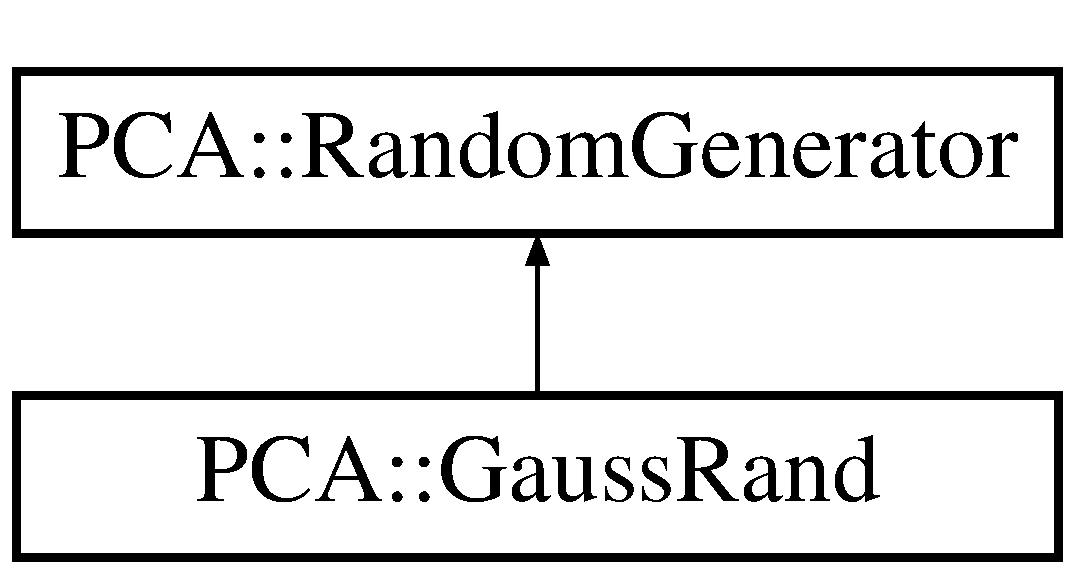
\includegraphics[height=2.000000cm]{class_p_c_a_1_1_gauss_rand}
\end{center}
\end{figure}
\subsection*{Public Member Functions}
\begin{DoxyCompactItemize}
\item 
\hyperlink{class_p_c_a_1_1_gauss_rand_a981fa1a94f0a38702117cc17c3cee549}{Gauss\+Rand} (double mean=0.\+0, double std\+Deviation=1.\+0)
\item 
\hyperlink{class_p_c_a_1_1_gauss_rand_aa5419fd06c7192c1d953f90bc38cff94}{$\sim$\+Gauss\+Rand} ()
\item 
virtual double \hyperlink{class_p_c_a_1_1_gauss_rand_a594130952a4999972f08b429ea6af959}{operator()} ()
\begin{DoxyCompactList}\small\item\em overloading operator () \end{DoxyCompactList}\end{DoxyCompactItemize}
\subsection*{Private Attributes}
\begin{DoxyCompactItemize}
\item 
std\+::normal\+\_\+distribution$<$ double $>$ \hyperlink{class_p_c_a_1_1_gauss_rand_a2a3c5494238db1cc94c2408227d9dbed}{distribution}
\end{DoxyCompactItemize}
\subsection*{Additional Inherited Members}


\subsection{Constructor \& Destructor Documentation}
\hypertarget{class_p_c_a_1_1_gauss_rand_a981fa1a94f0a38702117cc17c3cee549}{}\label{class_p_c_a_1_1_gauss_rand_a981fa1a94f0a38702117cc17c3cee549} 
\index{P\+C\+A\+::\+Gauss\+Rand@{P\+C\+A\+::\+Gauss\+Rand}!Gauss\+Rand@{Gauss\+Rand}}
\index{Gauss\+Rand@{Gauss\+Rand}!P\+C\+A\+::\+Gauss\+Rand@{P\+C\+A\+::\+Gauss\+Rand}}
\subsubsection{\texorpdfstring{Gauss\+Rand()}{GaussRand()}}
{\footnotesize\ttfamily P\+C\+A\+::\+Gauss\+Rand\+::\+Gauss\+Rand (\begin{DoxyParamCaption}\item[{double}]{mean = {\ttfamily 0.0},  }\item[{double}]{std\+Deviation = {\ttfamily 1.0} }\end{DoxyParamCaption})}

\hypertarget{class_p_c_a_1_1_gauss_rand_aa5419fd06c7192c1d953f90bc38cff94}{}\label{class_p_c_a_1_1_gauss_rand_aa5419fd06c7192c1d953f90bc38cff94} 
\index{P\+C\+A\+::\+Gauss\+Rand@{P\+C\+A\+::\+Gauss\+Rand}!````~Gauss\+Rand@{$\sim$\+Gauss\+Rand}}
\index{````~Gauss\+Rand@{$\sim$\+Gauss\+Rand}!P\+C\+A\+::\+Gauss\+Rand@{P\+C\+A\+::\+Gauss\+Rand}}
\subsubsection{\texorpdfstring{$\sim$\+Gauss\+Rand()}{~GaussRand()}}
{\footnotesize\ttfamily P\+C\+A\+::\+Gauss\+Rand\+::$\sim$\+Gauss\+Rand (\begin{DoxyParamCaption}{ }\end{DoxyParamCaption})}



\subsection{Member Function Documentation}
\hypertarget{class_p_c_a_1_1_gauss_rand_a594130952a4999972f08b429ea6af959}{}\label{class_p_c_a_1_1_gauss_rand_a594130952a4999972f08b429ea6af959} 
\index{P\+C\+A\+::\+Gauss\+Rand@{P\+C\+A\+::\+Gauss\+Rand}!operator()@{operator()}}
\index{operator()@{operator()}!P\+C\+A\+::\+Gauss\+Rand@{P\+C\+A\+::\+Gauss\+Rand}}
\subsubsection{\texorpdfstring{operator()()}{operator()()}}
{\footnotesize\ttfamily double P\+C\+A\+::\+Gauss\+Rand\+::operator() (\begin{DoxyParamCaption}{ }\end{DoxyParamCaption})\hspace{0.3cm}{\ttfamily [virtual]}}



overloading operator () 



Implements \hyperlink{class_p_c_a_1_1_random_generator_a4361e39397900ae1e7b2cfa91a592509}{P\+C\+A\+::\+Random\+Generator}.



\subsection{Member Data Documentation}
\hypertarget{class_p_c_a_1_1_gauss_rand_a2a3c5494238db1cc94c2408227d9dbed}{}\label{class_p_c_a_1_1_gauss_rand_a2a3c5494238db1cc94c2408227d9dbed} 
\index{P\+C\+A\+::\+Gauss\+Rand@{P\+C\+A\+::\+Gauss\+Rand}!distribution@{distribution}}
\index{distribution@{distribution}!P\+C\+A\+::\+Gauss\+Rand@{P\+C\+A\+::\+Gauss\+Rand}}
\subsubsection{\texorpdfstring{distribution}{distribution}}
{\footnotesize\ttfamily std\+::normal\+\_\+distribution$<$double$>$ P\+C\+A\+::\+Gauss\+Rand\+::distribution\hspace{0.3cm}{\ttfamily [private]}}



The documentation for this class was generated from the following files\+:\begin{DoxyCompactItemize}
\item 
/\+Users/annsi118/\+Documents/\+Git\+\_\+projects/\+P\+C\+M\+C/\+P\+C\+M\+C\+\_\+lib/include/\+Random/\hyperlink{_gauss_rand_8h}{Gauss\+Rand.\+h}\item 
/\+Users/annsi118/\+Documents/\+Git\+\_\+projects/\+P\+C\+M\+C/\+P\+C\+M\+C\+\_\+lib/source/\+Random/\hyperlink{_gauss_rand_8cpp}{Gauss\+Rand.\+cpp}\end{DoxyCompactItemize}

\hypertarget{class_p_c_a_1_1_hamiltonian}{}\section{P\+CA\+:\+:Hamiltonian Class Reference}
\label{class_p_c_a_1_1_hamiltonian}\index{P\+C\+A\+::\+Hamiltonian@{P\+C\+A\+::\+Hamiltonian}}


\hyperlink{class_p_c_a_1_1_hamiltonian}{Hamiltonian}.  




{\ttfamily \#include $<$Hamiltonian.\+h$>$}

\subsection*{Public Member Functions}
\begin{DoxyCompactItemize}
\item 
\hyperlink{class_p_c_a_1_1_hamiltonian_a3010d0e945bf871c22e57d530783c02a}{Hamiltonian} (int num\+Sites\+\_\+in)
\item 
\hyperlink{class_p_c_a_1_1_hamiltonian_ad2663a98cb52b4675ed01d6b911dd45a}{Hamiltonian} (int num\+Sites\+\_\+in, double q\+\_\+in, double m\+\_\+in, double c\+\_\+in, double d\+\_\+in, double a\+\_\+in, double b\+\_\+in=0, double alpha\+\_\+in=1.\+0, double mu\+\_\+in=0)
\begin{DoxyCompactList}\small\item\em Constructor for homopolymer. \end{DoxyCompactList}\item 
bool \hyperlink{class_p_c_a_1_1_hamiltonian_a3c9bddc6635c2a5a2ba0b2956126eb79}{check\+All\+Param\+Are\+Seted} ()
\item 
\hyperlink{class_p_c_a_1_1_hamiltonian_a87dcca06e1580312d8ffd4ef7fcad219}{$\sim$\+Hamiltonian} ()
\item 
double \hyperlink{class_p_c_a_1_1_hamiltonian_aaf2a99fc482ccd2ebb0dc671f1a8df5a}{energy\+One\+Site} (int site, const \hyperlink{class_p_c_a_1_1_polymer_m_c}{Polymer\+MC} \&\hyperlink{classpolymer}{polymer}) const
\item 
double \hyperlink{class_p_c_a_1_1_hamiltonian_a0751ca31444a5de38e6e5d7d07843538}{energy\+All\+Sites} (const \hyperlink{class_p_c_a_1_1_polymer_m_c}{Polymer\+MC} \&\hyperlink{classpolymer}{polymer}) const
\item 
double \hyperlink{class_p_c_a_1_1_hamiltonian_ad940f8b79c95c45ba11fe21f9491240b}{generate\+Tau} (double kappa\+\_\+i, double T) const
\begin{DoxyCompactList}\small\item\em Generate tau according Gaussian distribution. \end{DoxyCompactList}\end{DoxyCompactItemize}
\begin{Indent}{\bf Push functions (fills arrays including from\+Site and to\+Site!)\+:}\par
\begin{DoxyCompactItemize}
\item 
void \hyperlink{class_p_c_a_1_1_hamiltonian_aa1acb10e2078e74b747892db50a0342c}{push\+Alpha} (double alpha\+\_\+in)
\item 
void \hyperlink{class_p_c_a_1_1_hamiltonian_a98a0769af6bbaae97843e821b9b516a1}{push\+Mu} (double mu\+\_\+in)
\item 
void \hyperlink{class_p_c_a_1_1_hamiltonian_acc90d71bea33d377b93db657f4444d93}{pushQ} (double q\+\_\+in, int from\+Site, int to\+Site)
\item 
void \hyperlink{class_p_c_a_1_1_hamiltonian_a65c8f6848095abff386aa04a916b0c81}{pushM} (double m\+\_\+in, int from\+Site, int to\+Site)
\item 
void \hyperlink{class_p_c_a_1_1_hamiltonian_a9ca9ef677e2fedc8d82faca80e216e17}{pushC} (double c\+\_\+in, int from\+Site, int to\+Site)
\item 
void \hyperlink{class_p_c_a_1_1_hamiltonian_a8f0f25f18c67f7943714d086737e427f}{pushD} (double d\+\_\+in, int from\+Site, int to\+Site)
\item 
void \hyperlink{class_p_c_a_1_1_hamiltonian_aacf57a40855dbf2e27f598b0af2fcba3}{pushA} (double a\+\_\+in, int from\+Site, int to\+Site)
\item 
void \hyperlink{class_p_c_a_1_1_hamiltonian_a5390261dba56862d9ce18d0102f81ce1}{pushB} (double b\+\_\+in, int from\+Site, int to\+Site)
\end{DoxyCompactItemize}
\end{Indent}
\subsection*{Private Attributes}
\begin{DoxyCompactItemize}
\item 
int \hyperlink{class_p_c_a_1_1_hamiltonian_ad974eb16fba08e8e07cd60756fd223fb}{num\+Sites}
\item 
double \hyperlink{class_p_c_a_1_1_hamiltonian_a71a66a52512faafc9bc8594d96f02e5f}{alpha}
\item 
double \hyperlink{class_p_c_a_1_1_hamiltonian_afe68ce905e666835d5f1042c15be14bc}{mu}
\item 
double $\ast$ \hyperlink{class_p_c_a_1_1_hamiltonian_a2ff873d072df1447deb904d615fe9f02}{q}
\item 
double $\ast$ \hyperlink{class_p_c_a_1_1_hamiltonian_a6f5a67ef0c252c98edf24637179dbbc7}{m}
\item 
double $\ast$ \hyperlink{class_p_c_a_1_1_hamiltonian_ada70e13b8ae935e2109179d50fcfaa2f}{c}
\item 
double $\ast$ \hyperlink{class_p_c_a_1_1_hamiltonian_a61b0c483fb1966a22eaed55cca41950d}{d}
\item 
double $\ast$ \hyperlink{class_p_c_a_1_1_hamiltonian_aec8578a7d250be77a3e2eb84718815c7}{a}
\item 
double $\ast$ \hyperlink{class_p_c_a_1_1_hamiltonian_ac3a46f259db252d1b3a4ddbf40422026}{b}
\end{DoxyCompactItemize}


\subsection{Detailed Description}
\hyperlink{class_p_c_a_1_1_hamiltonian}{Hamiltonian}. 

\[ H=-\sum_{i=1}^{N-1} (2+\mu)\kappa_{i+1} \kappa_i + \alpha\sum_{i=1}^{N} \left\{ 2\kappa_i ^2 + q ( \kappa_i^2-m^2)^2+ \frac{c}{2}(d \kappa_i^2+1) \tau^2-a(b\kappa_i^2+1)\tau_i\right\} \] 

\subsection{Constructor \& Destructor Documentation}
\hypertarget{class_p_c_a_1_1_hamiltonian_a3010d0e945bf871c22e57d530783c02a}{}\label{class_p_c_a_1_1_hamiltonian_a3010d0e945bf871c22e57d530783c02a} 
\index{P\+C\+A\+::\+Hamiltonian@{P\+C\+A\+::\+Hamiltonian}!Hamiltonian@{Hamiltonian}}
\index{Hamiltonian@{Hamiltonian}!P\+C\+A\+::\+Hamiltonian@{P\+C\+A\+::\+Hamiltonian}}
\subsubsection{\texorpdfstring{Hamiltonian()}{Hamiltonian()}\hspace{0.1cm}{\footnotesize\ttfamily [1/2]}}
{\footnotesize\ttfamily P\+C\+A\+::\+Hamiltonian\+::\+Hamiltonian (\begin{DoxyParamCaption}\item[{int}]{num\+Sites\+\_\+in }\end{DoxyParamCaption})}

\hypertarget{class_p_c_a_1_1_hamiltonian_ad2663a98cb52b4675ed01d6b911dd45a}{}\label{class_p_c_a_1_1_hamiltonian_ad2663a98cb52b4675ed01d6b911dd45a} 
\index{P\+C\+A\+::\+Hamiltonian@{P\+C\+A\+::\+Hamiltonian}!Hamiltonian@{Hamiltonian}}
\index{Hamiltonian@{Hamiltonian}!P\+C\+A\+::\+Hamiltonian@{P\+C\+A\+::\+Hamiltonian}}
\subsubsection{\texorpdfstring{Hamiltonian()}{Hamiltonian()}\hspace{0.1cm}{\footnotesize\ttfamily [2/2]}}
{\footnotesize\ttfamily P\+C\+A\+::\+Hamiltonian\+::\+Hamiltonian (\begin{DoxyParamCaption}\item[{int}]{num\+Sites\+\_\+in,  }\item[{double}]{q\+\_\+in,  }\item[{double}]{m\+\_\+in,  }\item[{double}]{c\+\_\+in,  }\item[{double}]{d\+\_\+in,  }\item[{double}]{a\+\_\+in,  }\item[{double}]{b\+\_\+in = {\ttfamily 0},  }\item[{double}]{alpha\+\_\+in = {\ttfamily 1.0},  }\item[{double}]{mu\+\_\+in = {\ttfamily 0} }\end{DoxyParamCaption})}



Constructor for homopolymer. 

\hypertarget{class_p_c_a_1_1_hamiltonian_a87dcca06e1580312d8ffd4ef7fcad219}{}\label{class_p_c_a_1_1_hamiltonian_a87dcca06e1580312d8ffd4ef7fcad219} 
\index{P\+C\+A\+::\+Hamiltonian@{P\+C\+A\+::\+Hamiltonian}!````~Hamiltonian@{$\sim$\+Hamiltonian}}
\index{````~Hamiltonian@{$\sim$\+Hamiltonian}!P\+C\+A\+::\+Hamiltonian@{P\+C\+A\+::\+Hamiltonian}}
\subsubsection{\texorpdfstring{$\sim$\+Hamiltonian()}{~Hamiltonian()}}
{\footnotesize\ttfamily P\+C\+A\+::\+Hamiltonian\+::$\sim$\+Hamiltonian (\begin{DoxyParamCaption}{ }\end{DoxyParamCaption})}



\subsection{Member Function Documentation}
\hypertarget{class_p_c_a_1_1_hamiltonian_a3c9bddc6635c2a5a2ba0b2956126eb79}{}\label{class_p_c_a_1_1_hamiltonian_a3c9bddc6635c2a5a2ba0b2956126eb79} 
\index{P\+C\+A\+::\+Hamiltonian@{P\+C\+A\+::\+Hamiltonian}!check\+All\+Param\+Are\+Seted@{check\+All\+Param\+Are\+Seted}}
\index{check\+All\+Param\+Are\+Seted@{check\+All\+Param\+Are\+Seted}!P\+C\+A\+::\+Hamiltonian@{P\+C\+A\+::\+Hamiltonian}}
\subsubsection{\texorpdfstring{check\+All\+Param\+Are\+Seted()}{checkAllParamAreSeted()}}
{\footnotesize\ttfamily bool P\+C\+A\+::\+Hamiltonian\+::check\+All\+Param\+Are\+Seted (\begin{DoxyParamCaption}{ }\end{DoxyParamCaption})}

\hypertarget{class_p_c_a_1_1_hamiltonian_a0751ca31444a5de38e6e5d7d07843538}{}\label{class_p_c_a_1_1_hamiltonian_a0751ca31444a5de38e6e5d7d07843538} 
\index{P\+C\+A\+::\+Hamiltonian@{P\+C\+A\+::\+Hamiltonian}!energy\+All\+Sites@{energy\+All\+Sites}}
\index{energy\+All\+Sites@{energy\+All\+Sites}!P\+C\+A\+::\+Hamiltonian@{P\+C\+A\+::\+Hamiltonian}}
\subsubsection{\texorpdfstring{energy\+All\+Sites()}{energyAllSites()}}
{\footnotesize\ttfamily double P\+C\+A\+::\+Hamiltonian\+::energy\+All\+Sites (\begin{DoxyParamCaption}\item[{const \hyperlink{class_p_c_a_1_1_polymer_m_c}{Polymer\+MC} \&}]{polymer }\end{DoxyParamCaption}) const}

\hypertarget{class_p_c_a_1_1_hamiltonian_aaf2a99fc482ccd2ebb0dc671f1a8df5a}{}\label{class_p_c_a_1_1_hamiltonian_aaf2a99fc482ccd2ebb0dc671f1a8df5a} 
\index{P\+C\+A\+::\+Hamiltonian@{P\+C\+A\+::\+Hamiltonian}!energy\+One\+Site@{energy\+One\+Site}}
\index{energy\+One\+Site@{energy\+One\+Site}!P\+C\+A\+::\+Hamiltonian@{P\+C\+A\+::\+Hamiltonian}}
\subsubsection{\texorpdfstring{energy\+One\+Site()}{energyOneSite()}}
{\footnotesize\ttfamily double P\+C\+A\+::\+Hamiltonian\+::energy\+One\+Site (\begin{DoxyParamCaption}\item[{int}]{site,  }\item[{const \hyperlink{class_p_c_a_1_1_polymer_m_c}{Polymer\+MC} \&}]{polymer }\end{DoxyParamCaption}) const}

\hypertarget{class_p_c_a_1_1_hamiltonian_ad940f8b79c95c45ba11fe21f9491240b}{}\label{class_p_c_a_1_1_hamiltonian_ad940f8b79c95c45ba11fe21f9491240b} 
\index{P\+C\+A\+::\+Hamiltonian@{P\+C\+A\+::\+Hamiltonian}!generate\+Tau@{generate\+Tau}}
\index{generate\+Tau@{generate\+Tau}!P\+C\+A\+::\+Hamiltonian@{P\+C\+A\+::\+Hamiltonian}}
\subsubsection{\texorpdfstring{generate\+Tau()}{generateTau()}}
{\footnotesize\ttfamily double P\+C\+A\+::\+Hamiltonian\+::generate\+Tau (\begin{DoxyParamCaption}\item[{double}]{kappa\+\_\+i,  }\item[{double}]{T }\end{DoxyParamCaption}) const}



Generate tau according Gaussian distribution. 

\[P\sim \exp\left(-\frac{(\tau_i-\mu)^2}{2\sigma^2}\right)\] Coefficients\+: \[\mu=\frac{a(b\kappa_i^2+1)}{c(d\kappa_i^2+1)}\] \[\sigma^2=\frac{T}{\alpha c(d\kappa_i^2+1)}\] \hypertarget{class_p_c_a_1_1_hamiltonian_aacf57a40855dbf2e27f598b0af2fcba3}{}\label{class_p_c_a_1_1_hamiltonian_aacf57a40855dbf2e27f598b0af2fcba3} 
\index{P\+C\+A\+::\+Hamiltonian@{P\+C\+A\+::\+Hamiltonian}!pushA@{pushA}}
\index{pushA@{pushA}!P\+C\+A\+::\+Hamiltonian@{P\+C\+A\+::\+Hamiltonian}}
\subsubsection{\texorpdfstring{push\+A()}{pushA()}}
{\footnotesize\ttfamily void P\+C\+A\+::\+Hamiltonian\+::pushA (\begin{DoxyParamCaption}\item[{double}]{a\+\_\+in,  }\item[{int}]{from\+Site,  }\item[{int}]{to\+Site }\end{DoxyParamCaption})}

\hypertarget{class_p_c_a_1_1_hamiltonian_aa1acb10e2078e74b747892db50a0342c}{}\label{class_p_c_a_1_1_hamiltonian_aa1acb10e2078e74b747892db50a0342c} 
\index{P\+C\+A\+::\+Hamiltonian@{P\+C\+A\+::\+Hamiltonian}!push\+Alpha@{push\+Alpha}}
\index{push\+Alpha@{push\+Alpha}!P\+C\+A\+::\+Hamiltonian@{P\+C\+A\+::\+Hamiltonian}}
\subsubsection{\texorpdfstring{push\+Alpha()}{pushAlpha()}}
{\footnotesize\ttfamily void P\+C\+A\+::\+Hamiltonian\+::push\+Alpha (\begin{DoxyParamCaption}\item[{double}]{alpha\+\_\+in }\end{DoxyParamCaption})}

\hypertarget{class_p_c_a_1_1_hamiltonian_a5390261dba56862d9ce18d0102f81ce1}{}\label{class_p_c_a_1_1_hamiltonian_a5390261dba56862d9ce18d0102f81ce1} 
\index{P\+C\+A\+::\+Hamiltonian@{P\+C\+A\+::\+Hamiltonian}!pushB@{pushB}}
\index{pushB@{pushB}!P\+C\+A\+::\+Hamiltonian@{P\+C\+A\+::\+Hamiltonian}}
\subsubsection{\texorpdfstring{push\+B()}{pushB()}}
{\footnotesize\ttfamily void P\+C\+A\+::\+Hamiltonian\+::pushB (\begin{DoxyParamCaption}\item[{double}]{b\+\_\+in,  }\item[{int}]{from\+Site,  }\item[{int}]{to\+Site }\end{DoxyParamCaption})}

\hypertarget{class_p_c_a_1_1_hamiltonian_a9ca9ef677e2fedc8d82faca80e216e17}{}\label{class_p_c_a_1_1_hamiltonian_a9ca9ef677e2fedc8d82faca80e216e17} 
\index{P\+C\+A\+::\+Hamiltonian@{P\+C\+A\+::\+Hamiltonian}!pushC@{pushC}}
\index{pushC@{pushC}!P\+C\+A\+::\+Hamiltonian@{P\+C\+A\+::\+Hamiltonian}}
\subsubsection{\texorpdfstring{push\+C()}{pushC()}}
{\footnotesize\ttfamily void P\+C\+A\+::\+Hamiltonian\+::pushC (\begin{DoxyParamCaption}\item[{double}]{c\+\_\+in,  }\item[{int}]{from\+Site,  }\item[{int}]{to\+Site }\end{DoxyParamCaption})}

\hypertarget{class_p_c_a_1_1_hamiltonian_a8f0f25f18c67f7943714d086737e427f}{}\label{class_p_c_a_1_1_hamiltonian_a8f0f25f18c67f7943714d086737e427f} 
\index{P\+C\+A\+::\+Hamiltonian@{P\+C\+A\+::\+Hamiltonian}!pushD@{pushD}}
\index{pushD@{pushD}!P\+C\+A\+::\+Hamiltonian@{P\+C\+A\+::\+Hamiltonian}}
\subsubsection{\texorpdfstring{push\+D()}{pushD()}}
{\footnotesize\ttfamily void P\+C\+A\+::\+Hamiltonian\+::pushD (\begin{DoxyParamCaption}\item[{double}]{d\+\_\+in,  }\item[{int}]{from\+Site,  }\item[{int}]{to\+Site }\end{DoxyParamCaption})}

\hypertarget{class_p_c_a_1_1_hamiltonian_a65c8f6848095abff386aa04a916b0c81}{}\label{class_p_c_a_1_1_hamiltonian_a65c8f6848095abff386aa04a916b0c81} 
\index{P\+C\+A\+::\+Hamiltonian@{P\+C\+A\+::\+Hamiltonian}!pushM@{pushM}}
\index{pushM@{pushM}!P\+C\+A\+::\+Hamiltonian@{P\+C\+A\+::\+Hamiltonian}}
\subsubsection{\texorpdfstring{push\+M()}{pushM()}}
{\footnotesize\ttfamily void P\+C\+A\+::\+Hamiltonian\+::pushM (\begin{DoxyParamCaption}\item[{double}]{m\+\_\+in,  }\item[{int}]{from\+Site,  }\item[{int}]{to\+Site }\end{DoxyParamCaption})}

\hypertarget{class_p_c_a_1_1_hamiltonian_a98a0769af6bbaae97843e821b9b516a1}{}\label{class_p_c_a_1_1_hamiltonian_a98a0769af6bbaae97843e821b9b516a1} 
\index{P\+C\+A\+::\+Hamiltonian@{P\+C\+A\+::\+Hamiltonian}!push\+Mu@{push\+Mu}}
\index{push\+Mu@{push\+Mu}!P\+C\+A\+::\+Hamiltonian@{P\+C\+A\+::\+Hamiltonian}}
\subsubsection{\texorpdfstring{push\+Mu()}{pushMu()}}
{\footnotesize\ttfamily void P\+C\+A\+::\+Hamiltonian\+::push\+Mu (\begin{DoxyParamCaption}\item[{double}]{mu\+\_\+in }\end{DoxyParamCaption})}

\hypertarget{class_p_c_a_1_1_hamiltonian_acc90d71bea33d377b93db657f4444d93}{}\label{class_p_c_a_1_1_hamiltonian_acc90d71bea33d377b93db657f4444d93} 
\index{P\+C\+A\+::\+Hamiltonian@{P\+C\+A\+::\+Hamiltonian}!pushQ@{pushQ}}
\index{pushQ@{pushQ}!P\+C\+A\+::\+Hamiltonian@{P\+C\+A\+::\+Hamiltonian}}
\subsubsection{\texorpdfstring{push\+Q()}{pushQ()}}
{\footnotesize\ttfamily void P\+C\+A\+::\+Hamiltonian\+::pushQ (\begin{DoxyParamCaption}\item[{double}]{q\+\_\+in,  }\item[{int}]{from\+Site,  }\item[{int}]{to\+Site }\end{DoxyParamCaption})}



\subsection{Member Data Documentation}
\hypertarget{class_p_c_a_1_1_hamiltonian_aec8578a7d250be77a3e2eb84718815c7}{}\label{class_p_c_a_1_1_hamiltonian_aec8578a7d250be77a3e2eb84718815c7} 
\index{P\+C\+A\+::\+Hamiltonian@{P\+C\+A\+::\+Hamiltonian}!a@{a}}
\index{a@{a}!P\+C\+A\+::\+Hamiltonian@{P\+C\+A\+::\+Hamiltonian}}
\subsubsection{\texorpdfstring{a}{a}}
{\footnotesize\ttfamily double$\ast$ P\+C\+A\+::\+Hamiltonian\+::a\hspace{0.3cm}{\ttfamily [private]}}

\hypertarget{class_p_c_a_1_1_hamiltonian_a71a66a52512faafc9bc8594d96f02e5f}{}\label{class_p_c_a_1_1_hamiltonian_a71a66a52512faafc9bc8594d96f02e5f} 
\index{P\+C\+A\+::\+Hamiltonian@{P\+C\+A\+::\+Hamiltonian}!alpha@{alpha}}
\index{alpha@{alpha}!P\+C\+A\+::\+Hamiltonian@{P\+C\+A\+::\+Hamiltonian}}
\subsubsection{\texorpdfstring{alpha}{alpha}}
{\footnotesize\ttfamily double P\+C\+A\+::\+Hamiltonian\+::alpha\hspace{0.3cm}{\ttfamily [private]}}

\hypertarget{class_p_c_a_1_1_hamiltonian_ac3a46f259db252d1b3a4ddbf40422026}{}\label{class_p_c_a_1_1_hamiltonian_ac3a46f259db252d1b3a4ddbf40422026} 
\index{P\+C\+A\+::\+Hamiltonian@{P\+C\+A\+::\+Hamiltonian}!b@{b}}
\index{b@{b}!P\+C\+A\+::\+Hamiltonian@{P\+C\+A\+::\+Hamiltonian}}
\subsubsection{\texorpdfstring{b}{b}}
{\footnotesize\ttfamily double$\ast$ P\+C\+A\+::\+Hamiltonian\+::b\hspace{0.3cm}{\ttfamily [private]}}

\hypertarget{class_p_c_a_1_1_hamiltonian_ada70e13b8ae935e2109179d50fcfaa2f}{}\label{class_p_c_a_1_1_hamiltonian_ada70e13b8ae935e2109179d50fcfaa2f} 
\index{P\+C\+A\+::\+Hamiltonian@{P\+C\+A\+::\+Hamiltonian}!c@{c}}
\index{c@{c}!P\+C\+A\+::\+Hamiltonian@{P\+C\+A\+::\+Hamiltonian}}
\subsubsection{\texorpdfstring{c}{c}}
{\footnotesize\ttfamily double$\ast$ P\+C\+A\+::\+Hamiltonian\+::c\hspace{0.3cm}{\ttfamily [private]}}

\hypertarget{class_p_c_a_1_1_hamiltonian_a61b0c483fb1966a22eaed55cca41950d}{}\label{class_p_c_a_1_1_hamiltonian_a61b0c483fb1966a22eaed55cca41950d} 
\index{P\+C\+A\+::\+Hamiltonian@{P\+C\+A\+::\+Hamiltonian}!d@{d}}
\index{d@{d}!P\+C\+A\+::\+Hamiltonian@{P\+C\+A\+::\+Hamiltonian}}
\subsubsection{\texorpdfstring{d}{d}}
{\footnotesize\ttfamily double$\ast$ P\+C\+A\+::\+Hamiltonian\+::d\hspace{0.3cm}{\ttfamily [private]}}

\hypertarget{class_p_c_a_1_1_hamiltonian_a6f5a67ef0c252c98edf24637179dbbc7}{}\label{class_p_c_a_1_1_hamiltonian_a6f5a67ef0c252c98edf24637179dbbc7} 
\index{P\+C\+A\+::\+Hamiltonian@{P\+C\+A\+::\+Hamiltonian}!m@{m}}
\index{m@{m}!P\+C\+A\+::\+Hamiltonian@{P\+C\+A\+::\+Hamiltonian}}
\subsubsection{\texorpdfstring{m}{m}}
{\footnotesize\ttfamily double$\ast$ P\+C\+A\+::\+Hamiltonian\+::m\hspace{0.3cm}{\ttfamily [private]}}

\hypertarget{class_p_c_a_1_1_hamiltonian_afe68ce905e666835d5f1042c15be14bc}{}\label{class_p_c_a_1_1_hamiltonian_afe68ce905e666835d5f1042c15be14bc} 
\index{P\+C\+A\+::\+Hamiltonian@{P\+C\+A\+::\+Hamiltonian}!mu@{mu}}
\index{mu@{mu}!P\+C\+A\+::\+Hamiltonian@{P\+C\+A\+::\+Hamiltonian}}
\subsubsection{\texorpdfstring{mu}{mu}}
{\footnotesize\ttfamily double P\+C\+A\+::\+Hamiltonian\+::mu\hspace{0.3cm}{\ttfamily [private]}}

\hypertarget{class_p_c_a_1_1_hamiltonian_ad974eb16fba08e8e07cd60756fd223fb}{}\label{class_p_c_a_1_1_hamiltonian_ad974eb16fba08e8e07cd60756fd223fb} 
\index{P\+C\+A\+::\+Hamiltonian@{P\+C\+A\+::\+Hamiltonian}!num\+Sites@{num\+Sites}}
\index{num\+Sites@{num\+Sites}!P\+C\+A\+::\+Hamiltonian@{P\+C\+A\+::\+Hamiltonian}}
\subsubsection{\texorpdfstring{num\+Sites}{numSites}}
{\footnotesize\ttfamily int P\+C\+A\+::\+Hamiltonian\+::num\+Sites\hspace{0.3cm}{\ttfamily [private]}}

\hypertarget{class_p_c_a_1_1_hamiltonian_a2ff873d072df1447deb904d615fe9f02}{}\label{class_p_c_a_1_1_hamiltonian_a2ff873d072df1447deb904d615fe9f02} 
\index{P\+C\+A\+::\+Hamiltonian@{P\+C\+A\+::\+Hamiltonian}!q@{q}}
\index{q@{q}!P\+C\+A\+::\+Hamiltonian@{P\+C\+A\+::\+Hamiltonian}}
\subsubsection{\texorpdfstring{q}{q}}
{\footnotesize\ttfamily double$\ast$ P\+C\+A\+::\+Hamiltonian\+::q\hspace{0.3cm}{\ttfamily [private]}}



The documentation for this class was generated from the following files\+:\begin{DoxyCompactItemize}
\item 
/\+Users/annsi118/\+Documents/\+Git\+\_\+projects/\+P\+C\+M\+C/include/\+Energy/\hyperlink{_hamiltonian_8h}{Hamiltonian.\+h}\item 
/\+Users/annsi118/\+Documents/\+Git\+\_\+projects/\+P\+C\+M\+C/source/\+Energy/\hyperlink{_hamiltonian_8cpp}{Hamiltonian.\+cpp}\end{DoxyCompactItemize}

\hypertarget{class_p_c_a_1_1_hopping_amplitude_calculator}{}\section{P\+CA\+:\+:Hopping\+Amplitude\+Calculator Class Reference}
\label{class_p_c_a_1_1_hopping_amplitude_calculator}\index{P\+C\+A\+::\+Hopping\+Amplitude\+Calculator@{P\+C\+A\+::\+Hopping\+Amplitude\+Calculator}}


{\ttfamily \#include $<$Hopping\+Amplitude\+Calculator.\+h$>$}

Inheritance diagram for P\+CA\+:\+:Hopping\+Amplitude\+Calculator\+:\begin{figure}[H]
\begin{center}
\leavevmode
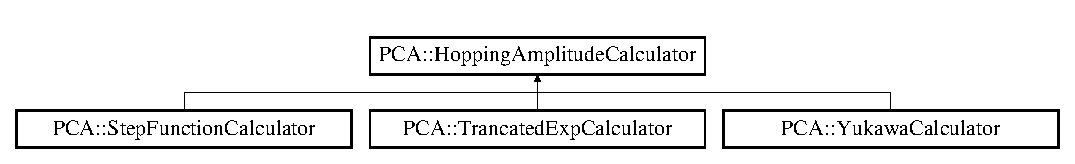
\includegraphics[height=1.761006cm]{class_p_c_a_1_1_hopping_amplitude_calculator}
\end{center}
\end{figure}
\subsection*{Public Member Functions}
\begin{DoxyCompactItemize}
\item 
virtual std\+::complex$<$ double $>$ \hyperlink{class_p_c_a_1_1_hopping_amplitude_calculator_ae925735be8ef006f3f8dfdc1a23cae89}{calculate\+HA} (double distance) const =0
\end{DoxyCompactItemize}


\subsection{Member Function Documentation}
\hypertarget{class_p_c_a_1_1_hopping_amplitude_calculator_ae925735be8ef006f3f8dfdc1a23cae89}{}\label{class_p_c_a_1_1_hopping_amplitude_calculator_ae925735be8ef006f3f8dfdc1a23cae89} 
\index{P\+C\+A\+::\+Hopping\+Amplitude\+Calculator@{P\+C\+A\+::\+Hopping\+Amplitude\+Calculator}!calculate\+HA@{calculate\+HA}}
\index{calculate\+HA@{calculate\+HA}!P\+C\+A\+::\+Hopping\+Amplitude\+Calculator@{P\+C\+A\+::\+Hopping\+Amplitude\+Calculator}}
\subsubsection{\texorpdfstring{calculate\+H\+A()}{calculateHA()}}
{\footnotesize\ttfamily virtual std\+::complex$<$double$>$ P\+C\+A\+::\+Hopping\+Amplitude\+Calculator\+::calculate\+HA (\begin{DoxyParamCaption}\item[{double}]{distance }\end{DoxyParamCaption}) const\hspace{0.3cm}{\ttfamily [pure virtual]}}



Implemented in \hyperlink{class_p_c_a_1_1_trancated_exp_calculator_afe48461b23fd2b0d350f32bdac0c3d18}{P\+C\+A\+::\+Trancated\+Exp\+Calculator}, \hyperlink{class_p_c_a_1_1_yukawa_calculator_a543f237d55350a7669f8b85789cae68d}{P\+C\+A\+::\+Yukawa\+Calculator}, and \hyperlink{class_p_c_a_1_1_step_function_calculator_a0607e2f78b6b7c0ed40083f921b58fdc}{P\+C\+A\+::\+Step\+Function\+Calculator}.



The documentation for this class was generated from the following file\+:\begin{DoxyCompactItemize}
\item 
/\+Users/annsi118/\+Documents/\+Git\+\_\+projects/\+P\+C\+M\+C/\+P\+C\+M\+C\+\_\+lib/include/\+Quantum/\hyperlink{_hopping_amplitude_calculator_8h}{Hopping\+Amplitude\+Calculator.\+h}\end{DoxyCompactItemize}

\hypertarget{classkappa__distribution}{}\section{kappa\+\_\+distribution Class Reference}
\label{classkappa__distribution}\index{kappa\+\_\+distribution@{kappa\+\_\+distribution}}


{\ttfamily \#include $<$prob\+\_\+distrib.\+h$>$}

\subsection*{Public Member Functions}
\begin{DoxyCompactItemize}
\item 
void \hyperlink{classkappa__distribution_abf97127e675e370e41c20a4bcf3920ce}{print\+\_\+stat} (F\+I\+LE $\ast$log\+\_\+file)
\item 
void \hyperlink{classkappa__distribution_a5e943b080c0c8a88e37a85100666cadb}{rand\+\_\+init} (int number)
\item 
int \hyperlink{classkappa__distribution_aaf5ceb9a7a92cd7cdb4ca07cf0f74388}{init} (double a\+\_\+in, double b\+\_\+in, double c\+\_\+in, double offset\+\_\+in)
\item 
double \hyperlink{classkappa__distribution_af8f5aef5827c9423c2d9c65a53a43202}{generate} ()
\item 
void \hyperlink{classkappa__distribution_ab18b8d4b45ba749340829da1ca18130c}{sort\+\_\+asc} ()
\item 
double \hyperlink{classkappa__distribution_a7e0171752a4a1c1b8b99950394281922}{polynom} (double x)
\item 
double \hyperlink{classkappa__distribution_ae7fee7da2f235cf8d319e00a7f8a4dc3}{der1} (double x)
\item 
double \hyperlink{classkappa__distribution_aafde4b907d4e201a59e3706ef5cb7c53}{der2} (double x)
\end{DoxyCompactItemize}
\subsection*{Public Attributes}
\begin{DoxyCompactItemize}
\item 
gsl\+\_\+rng $\ast$ \hyperlink{classkappa__distribution_a534c1be1b65e324fa62a733b3538196a}{mtrand}
\item 
double \hyperlink{classkappa__distribution_ac85c34598a6c6541660c024f509977c2}{a}
\item 
double \hyperlink{classkappa__distribution_ac9487f58886c93bede8d10f0660df323}{b}
\item 
double \hyperlink{classkappa__distribution_a90698395f61fde53725916a1405c2613}{c}
\item 
double \hyperlink{classkappa__distribution_aaf581ec013e458d9632689422352b575}{x1}
\item 
double \hyperlink{classkappa__distribution_a13e498d40d784837a04374e35d4ff4b7}{x2}
\item 
double \hyperlink{classkappa__distribution_add191b8968caa8c0f56806ab95ab9541}{x3}
\item 
int \hyperlink{classkappa__distribution_a437034eceb23e234b297882e74e65635}{n\+\_\+maximums}
\item 
double \hyperlink{classkappa__distribution_a1b1f2f453758df12ae36c45a2ef1442e}{x\+\_\+max1}
\item 
double \hyperlink{classkappa__distribution_a8ddb60e0b690eba68d3651975e0de470}{x\+\_\+max2}
\item 
double \hyperlink{classkappa__distribution_a4c5660bf0eb745115a97b763c400a2e7}{f\+\_\+max1}
\item 
double \hyperlink{classkappa__distribution_a197a28c1e2fb49e3ab2ba12fbf0b9de3}{f\+\_\+max2}
\item 
double \hyperlink{classkappa__distribution_ac1df2a43af198de04f20db0067754f31}{offset}
\item 
int \hyperlink{classkappa__distribution_a24fa777b043581c42d7b1219509bcef1}{n\+\_\+intervals}
\item 
double \hyperlink{classkappa__distribution_adabd36d6214f535740375a0bdf13f115}{kappa} \mbox{[}4\mbox{]}
\item 
double \hyperlink{classkappa__distribution_a6506e5322c9a9c919af36d9d34dbb180}{im\+\_\+epsilon}
\item 
double \hyperlink{classkappa__distribution_af7d9662cfb3cd567676f36785a3d15a1}{norm} \mbox{[}2\mbox{]}
\item 
int \hyperlink{classkappa__distribution_ab816226e269c7af719438350cebaf4eb}{N\+\_\+int\+\_\+steps}
\end{DoxyCompactItemize}


\subsection{Member Function Documentation}
\hypertarget{classkappa__distribution_ae7fee7da2f235cf8d319e00a7f8a4dc3}{}\label{classkappa__distribution_ae7fee7da2f235cf8d319e00a7f8a4dc3} 
\index{kappa\+\_\+distribution@{kappa\+\_\+distribution}!der1@{der1}}
\index{der1@{der1}!kappa\+\_\+distribution@{kappa\+\_\+distribution}}
\subsubsection{\texorpdfstring{der1()}{der1()}}
{\footnotesize\ttfamily double kappa\+\_\+distribution\+::der1 (\begin{DoxyParamCaption}\item[{double}]{x }\end{DoxyParamCaption})\hspace{0.3cm}{\ttfamily [inline]}}

\hypertarget{classkappa__distribution_aafde4b907d4e201a59e3706ef5cb7c53}{}\label{classkappa__distribution_aafde4b907d4e201a59e3706ef5cb7c53} 
\index{kappa\+\_\+distribution@{kappa\+\_\+distribution}!der2@{der2}}
\index{der2@{der2}!kappa\+\_\+distribution@{kappa\+\_\+distribution}}
\subsubsection{\texorpdfstring{der2()}{der2()}}
{\footnotesize\ttfamily double kappa\+\_\+distribution\+::der2 (\begin{DoxyParamCaption}\item[{double}]{x }\end{DoxyParamCaption})\hspace{0.3cm}{\ttfamily [inline]}}

\hypertarget{classkappa__distribution_af8f5aef5827c9423c2d9c65a53a43202}{}\label{classkappa__distribution_af8f5aef5827c9423c2d9c65a53a43202} 
\index{kappa\+\_\+distribution@{kappa\+\_\+distribution}!generate@{generate}}
\index{generate@{generate}!kappa\+\_\+distribution@{kappa\+\_\+distribution}}
\subsubsection{\texorpdfstring{generate()}{generate()}}
{\footnotesize\ttfamily double kappa\+\_\+distribution\+::generate (\begin{DoxyParamCaption}{ }\end{DoxyParamCaption})\hspace{0.3cm}{\ttfamily [inline]}}

\hypertarget{classkappa__distribution_aaf5ceb9a7a92cd7cdb4ca07cf0f74388}{}\label{classkappa__distribution_aaf5ceb9a7a92cd7cdb4ca07cf0f74388} 
\index{kappa\+\_\+distribution@{kappa\+\_\+distribution}!init@{init}}
\index{init@{init}!kappa\+\_\+distribution@{kappa\+\_\+distribution}}
\subsubsection{\texorpdfstring{init()}{init()}}
{\footnotesize\ttfamily int kappa\+\_\+distribution\+::init (\begin{DoxyParamCaption}\item[{double}]{a\+\_\+in,  }\item[{double}]{b\+\_\+in,  }\item[{double}]{c\+\_\+in,  }\item[{double}]{offset\+\_\+in }\end{DoxyParamCaption})\hspace{0.3cm}{\ttfamily [inline]}}

\hypertarget{classkappa__distribution_a7e0171752a4a1c1b8b99950394281922}{}\label{classkappa__distribution_a7e0171752a4a1c1b8b99950394281922} 
\index{kappa\+\_\+distribution@{kappa\+\_\+distribution}!polynom@{polynom}}
\index{polynom@{polynom}!kappa\+\_\+distribution@{kappa\+\_\+distribution}}
\subsubsection{\texorpdfstring{polynom()}{polynom()}}
{\footnotesize\ttfamily double kappa\+\_\+distribution\+::polynom (\begin{DoxyParamCaption}\item[{double}]{x }\end{DoxyParamCaption})\hspace{0.3cm}{\ttfamily [inline]}}

\hypertarget{classkappa__distribution_abf97127e675e370e41c20a4bcf3920ce}{}\label{classkappa__distribution_abf97127e675e370e41c20a4bcf3920ce} 
\index{kappa\+\_\+distribution@{kappa\+\_\+distribution}!print\+\_\+stat@{print\+\_\+stat}}
\index{print\+\_\+stat@{print\+\_\+stat}!kappa\+\_\+distribution@{kappa\+\_\+distribution}}
\subsubsection{\texorpdfstring{print\+\_\+stat()}{print\_stat()}}
{\footnotesize\ttfamily void kappa\+\_\+distribution\+::print\+\_\+stat (\begin{DoxyParamCaption}\item[{F\+I\+LE $\ast$}]{log\+\_\+file }\end{DoxyParamCaption})\hspace{0.3cm}{\ttfamily [inline]}}

\hypertarget{classkappa__distribution_a5e943b080c0c8a88e37a85100666cadb}{}\label{classkappa__distribution_a5e943b080c0c8a88e37a85100666cadb} 
\index{kappa\+\_\+distribution@{kappa\+\_\+distribution}!rand\+\_\+init@{rand\+\_\+init}}
\index{rand\+\_\+init@{rand\+\_\+init}!kappa\+\_\+distribution@{kappa\+\_\+distribution}}
\subsubsection{\texorpdfstring{rand\+\_\+init()}{rand\_init()}}
{\footnotesize\ttfamily void kappa\+\_\+distribution\+::rand\+\_\+init (\begin{DoxyParamCaption}\item[{int}]{number }\end{DoxyParamCaption})\hspace{0.3cm}{\ttfamily [inline]}}

\hypertarget{classkappa__distribution_ab18b8d4b45ba749340829da1ca18130c}{}\label{classkappa__distribution_ab18b8d4b45ba749340829da1ca18130c} 
\index{kappa\+\_\+distribution@{kappa\+\_\+distribution}!sort\+\_\+asc@{sort\+\_\+asc}}
\index{sort\+\_\+asc@{sort\+\_\+asc}!kappa\+\_\+distribution@{kappa\+\_\+distribution}}
\subsubsection{\texorpdfstring{sort\+\_\+asc()}{sort\_asc()}}
{\footnotesize\ttfamily void kappa\+\_\+distribution\+::sort\+\_\+asc (\begin{DoxyParamCaption}{ }\end{DoxyParamCaption})\hspace{0.3cm}{\ttfamily [inline]}}



\subsection{Member Data Documentation}
\hypertarget{classkappa__distribution_ac85c34598a6c6541660c024f509977c2}{}\label{classkappa__distribution_ac85c34598a6c6541660c024f509977c2} 
\index{kappa\+\_\+distribution@{kappa\+\_\+distribution}!a@{a}}
\index{a@{a}!kappa\+\_\+distribution@{kappa\+\_\+distribution}}
\subsubsection{\texorpdfstring{a}{a}}
{\footnotesize\ttfamily double kappa\+\_\+distribution\+::a}

\hypertarget{classkappa__distribution_ac9487f58886c93bede8d10f0660df323}{}\label{classkappa__distribution_ac9487f58886c93bede8d10f0660df323} 
\index{kappa\+\_\+distribution@{kappa\+\_\+distribution}!b@{b}}
\index{b@{b}!kappa\+\_\+distribution@{kappa\+\_\+distribution}}
\subsubsection{\texorpdfstring{b}{b}}
{\footnotesize\ttfamily double kappa\+\_\+distribution\+::b}

\hypertarget{classkappa__distribution_a90698395f61fde53725916a1405c2613}{}\label{classkappa__distribution_a90698395f61fde53725916a1405c2613} 
\index{kappa\+\_\+distribution@{kappa\+\_\+distribution}!c@{c}}
\index{c@{c}!kappa\+\_\+distribution@{kappa\+\_\+distribution}}
\subsubsection{\texorpdfstring{c}{c}}
{\footnotesize\ttfamily double kappa\+\_\+distribution\+::c}

\hypertarget{classkappa__distribution_a4c5660bf0eb745115a97b763c400a2e7}{}\label{classkappa__distribution_a4c5660bf0eb745115a97b763c400a2e7} 
\index{kappa\+\_\+distribution@{kappa\+\_\+distribution}!f\+\_\+max1@{f\+\_\+max1}}
\index{f\+\_\+max1@{f\+\_\+max1}!kappa\+\_\+distribution@{kappa\+\_\+distribution}}
\subsubsection{\texorpdfstring{f\+\_\+max1}{f\_max1}}
{\footnotesize\ttfamily double kappa\+\_\+distribution\+::f\+\_\+max1}

\hypertarget{classkappa__distribution_a197a28c1e2fb49e3ab2ba12fbf0b9de3}{}\label{classkappa__distribution_a197a28c1e2fb49e3ab2ba12fbf0b9de3} 
\index{kappa\+\_\+distribution@{kappa\+\_\+distribution}!f\+\_\+max2@{f\+\_\+max2}}
\index{f\+\_\+max2@{f\+\_\+max2}!kappa\+\_\+distribution@{kappa\+\_\+distribution}}
\subsubsection{\texorpdfstring{f\+\_\+max2}{f\_max2}}
{\footnotesize\ttfamily double kappa\+\_\+distribution\+::f\+\_\+max2}

\hypertarget{classkappa__distribution_a6506e5322c9a9c919af36d9d34dbb180}{}\label{classkappa__distribution_a6506e5322c9a9c919af36d9d34dbb180} 
\index{kappa\+\_\+distribution@{kappa\+\_\+distribution}!im\+\_\+epsilon@{im\+\_\+epsilon}}
\index{im\+\_\+epsilon@{im\+\_\+epsilon}!kappa\+\_\+distribution@{kappa\+\_\+distribution}}
\subsubsection{\texorpdfstring{im\+\_\+epsilon}{im\_epsilon}}
{\footnotesize\ttfamily double kappa\+\_\+distribution\+::im\+\_\+epsilon}

\hypertarget{classkappa__distribution_adabd36d6214f535740375a0bdf13f115}{}\label{classkappa__distribution_adabd36d6214f535740375a0bdf13f115} 
\index{kappa\+\_\+distribution@{kappa\+\_\+distribution}!kappa@{kappa}}
\index{kappa@{kappa}!kappa\+\_\+distribution@{kappa\+\_\+distribution}}
\subsubsection{\texorpdfstring{kappa}{kappa}}
{\footnotesize\ttfamily double kappa\+\_\+distribution\+::kappa\mbox{[}4\mbox{]}}

\hypertarget{classkappa__distribution_a534c1be1b65e324fa62a733b3538196a}{}\label{classkappa__distribution_a534c1be1b65e324fa62a733b3538196a} 
\index{kappa\+\_\+distribution@{kappa\+\_\+distribution}!mtrand@{mtrand}}
\index{mtrand@{mtrand}!kappa\+\_\+distribution@{kappa\+\_\+distribution}}
\subsubsection{\texorpdfstring{mtrand}{mtrand}}
{\footnotesize\ttfamily gsl\+\_\+rng$\ast$ kappa\+\_\+distribution\+::mtrand}

\hypertarget{classkappa__distribution_ab816226e269c7af719438350cebaf4eb}{}\label{classkappa__distribution_ab816226e269c7af719438350cebaf4eb} 
\index{kappa\+\_\+distribution@{kappa\+\_\+distribution}!N\+\_\+int\+\_\+steps@{N\+\_\+int\+\_\+steps}}
\index{N\+\_\+int\+\_\+steps@{N\+\_\+int\+\_\+steps}!kappa\+\_\+distribution@{kappa\+\_\+distribution}}
\subsubsection{\texorpdfstring{N\+\_\+int\+\_\+steps}{N\_int\_steps}}
{\footnotesize\ttfamily int kappa\+\_\+distribution\+::\+N\+\_\+int\+\_\+steps}

\hypertarget{classkappa__distribution_a24fa777b043581c42d7b1219509bcef1}{}\label{classkappa__distribution_a24fa777b043581c42d7b1219509bcef1} 
\index{kappa\+\_\+distribution@{kappa\+\_\+distribution}!n\+\_\+intervals@{n\+\_\+intervals}}
\index{n\+\_\+intervals@{n\+\_\+intervals}!kappa\+\_\+distribution@{kappa\+\_\+distribution}}
\subsubsection{\texorpdfstring{n\+\_\+intervals}{n\_intervals}}
{\footnotesize\ttfamily int kappa\+\_\+distribution\+::n\+\_\+intervals}

\hypertarget{classkappa__distribution_a437034eceb23e234b297882e74e65635}{}\label{classkappa__distribution_a437034eceb23e234b297882e74e65635} 
\index{kappa\+\_\+distribution@{kappa\+\_\+distribution}!n\+\_\+maximums@{n\+\_\+maximums}}
\index{n\+\_\+maximums@{n\+\_\+maximums}!kappa\+\_\+distribution@{kappa\+\_\+distribution}}
\subsubsection{\texorpdfstring{n\+\_\+maximums}{n\_maximums}}
{\footnotesize\ttfamily int kappa\+\_\+distribution\+::n\+\_\+maximums}

\hypertarget{classkappa__distribution_af7d9662cfb3cd567676f36785a3d15a1}{}\label{classkappa__distribution_af7d9662cfb3cd567676f36785a3d15a1} 
\index{kappa\+\_\+distribution@{kappa\+\_\+distribution}!norm@{norm}}
\index{norm@{norm}!kappa\+\_\+distribution@{kappa\+\_\+distribution}}
\subsubsection{\texorpdfstring{norm}{norm}}
{\footnotesize\ttfamily double kappa\+\_\+distribution\+::norm\mbox{[}2\mbox{]}}

\hypertarget{classkappa__distribution_ac1df2a43af198de04f20db0067754f31}{}\label{classkappa__distribution_ac1df2a43af198de04f20db0067754f31} 
\index{kappa\+\_\+distribution@{kappa\+\_\+distribution}!offset@{offset}}
\index{offset@{offset}!kappa\+\_\+distribution@{kappa\+\_\+distribution}}
\subsubsection{\texorpdfstring{offset}{offset}}
{\footnotesize\ttfamily double kappa\+\_\+distribution\+::offset}

\hypertarget{classkappa__distribution_aaf581ec013e458d9632689422352b575}{}\label{classkappa__distribution_aaf581ec013e458d9632689422352b575} 
\index{kappa\+\_\+distribution@{kappa\+\_\+distribution}!x1@{x1}}
\index{x1@{x1}!kappa\+\_\+distribution@{kappa\+\_\+distribution}}
\subsubsection{\texorpdfstring{x1}{x1}}
{\footnotesize\ttfamily double kappa\+\_\+distribution\+::x1}

\hypertarget{classkappa__distribution_a13e498d40d784837a04374e35d4ff4b7}{}\label{classkappa__distribution_a13e498d40d784837a04374e35d4ff4b7} 
\index{kappa\+\_\+distribution@{kappa\+\_\+distribution}!x2@{x2}}
\index{x2@{x2}!kappa\+\_\+distribution@{kappa\+\_\+distribution}}
\subsubsection{\texorpdfstring{x2}{x2}}
{\footnotesize\ttfamily double kappa\+\_\+distribution\+::x2}

\hypertarget{classkappa__distribution_add191b8968caa8c0f56806ab95ab9541}{}\label{classkappa__distribution_add191b8968caa8c0f56806ab95ab9541} 
\index{kappa\+\_\+distribution@{kappa\+\_\+distribution}!x3@{x3}}
\index{x3@{x3}!kappa\+\_\+distribution@{kappa\+\_\+distribution}}
\subsubsection{\texorpdfstring{x3}{x3}}
{\footnotesize\ttfamily double kappa\+\_\+distribution\+::x3}

\hypertarget{classkappa__distribution_a1b1f2f453758df12ae36c45a2ef1442e}{}\label{classkappa__distribution_a1b1f2f453758df12ae36c45a2ef1442e} 
\index{kappa\+\_\+distribution@{kappa\+\_\+distribution}!x\+\_\+max1@{x\+\_\+max1}}
\index{x\+\_\+max1@{x\+\_\+max1}!kappa\+\_\+distribution@{kappa\+\_\+distribution}}
\subsubsection{\texorpdfstring{x\+\_\+max1}{x\_max1}}
{\footnotesize\ttfamily double kappa\+\_\+distribution\+::x\+\_\+max1}

\hypertarget{classkappa__distribution_a8ddb60e0b690eba68d3651975e0de470}{}\label{classkappa__distribution_a8ddb60e0b690eba68d3651975e0de470} 
\index{kappa\+\_\+distribution@{kappa\+\_\+distribution}!x\+\_\+max2@{x\+\_\+max2}}
\index{x\+\_\+max2@{x\+\_\+max2}!kappa\+\_\+distribution@{kappa\+\_\+distribution}}
\subsubsection{\texorpdfstring{x\+\_\+max2}{x\_max2}}
{\footnotesize\ttfamily double kappa\+\_\+distribution\+::x\+\_\+max2}



The documentation for this class was generated from the following file\+:\begin{DoxyCompactItemize}
\item 
/\+Users/annsi118/\+Documents/\+Git\+\_\+projects/\+P\+C\+M\+C/\hyperlink{prob__distrib_8h}{prob\+\_\+distrib.\+h}\end{DoxyCompactItemize}

\hypertarget{class_p_c_a_1_1_lennard_jones}{}\section{P\+CA\+:\+:Lennard\+Jones Class Reference}
\label{class_p_c_a_1_1_lennard_jones}\index{P\+C\+A\+::\+Lennard\+Jones@{P\+C\+A\+::\+Lennard\+Jones}}


Lennard-\/\+Jones potential.  




{\ttfamily \#include $<$Lennard\+Jones.\+h$>$}

\subsection*{Public Member Functions}
\begin{DoxyCompactItemize}
\item 
\hyperlink{class_p_c_a_1_1_lennard_jones_a177de9041d696f41ac2b498973047759}{Lennard\+Jones} (double gamma\+\_\+in, double r\+Min\+\_\+in)
\item 
\hyperlink{class_p_c_a_1_1_lennard_jones_ac8acfe0ebd2e7f263d6561ab515f0028}{$\sim$\+Lennard\+Jones} ()
\item 
double \hyperlink{class_p_c_a_1_1_lennard_jones_aa3ccc6cb511c3a10b1982c965a69e5be}{energy} (const \hyperlink{class_p_c_a_1_1_vector}{Vector} \&r)
\end{DoxyCompactItemize}
\subsection*{Private Attributes}
\begin{DoxyCompactItemize}
\item 
double \hyperlink{class_p_c_a_1_1_lennard_jones_ad28ea138038c2c43e9fd000752ea6130}{gamma}
\item 
double \hyperlink{class_p_c_a_1_1_lennard_jones_aa59f5f2bb7cf5c83a33a7f95d23ef4c8}{r\+Min}
\end{DoxyCompactItemize}


\subsection{Detailed Description}
Lennard-\/\+Jones potential. 

\[ U(r)= \gamma \left( \left(\frac{r_{min}}{r}\right)^{12} - 2 \left(\frac{r_{min}}{r}\right)^6\right)\] 

\subsection{Constructor \& Destructor Documentation}
\hypertarget{class_p_c_a_1_1_lennard_jones_a177de9041d696f41ac2b498973047759}{}\label{class_p_c_a_1_1_lennard_jones_a177de9041d696f41ac2b498973047759} 
\index{P\+C\+A\+::\+Lennard\+Jones@{P\+C\+A\+::\+Lennard\+Jones}!Lennard\+Jones@{Lennard\+Jones}}
\index{Lennard\+Jones@{Lennard\+Jones}!P\+C\+A\+::\+Lennard\+Jones@{P\+C\+A\+::\+Lennard\+Jones}}
\subsubsection{\texorpdfstring{Lennard\+Jones()}{LennardJones()}}
{\footnotesize\ttfamily P\+C\+A\+::\+Lennard\+Jones\+::\+Lennard\+Jones (\begin{DoxyParamCaption}\item[{double}]{gamma\+\_\+in,  }\item[{double}]{r\+Min\+\_\+in }\end{DoxyParamCaption})}

\hypertarget{class_p_c_a_1_1_lennard_jones_ac8acfe0ebd2e7f263d6561ab515f0028}{}\label{class_p_c_a_1_1_lennard_jones_ac8acfe0ebd2e7f263d6561ab515f0028} 
\index{P\+C\+A\+::\+Lennard\+Jones@{P\+C\+A\+::\+Lennard\+Jones}!````~Lennard\+Jones@{$\sim$\+Lennard\+Jones}}
\index{````~Lennard\+Jones@{$\sim$\+Lennard\+Jones}!P\+C\+A\+::\+Lennard\+Jones@{P\+C\+A\+::\+Lennard\+Jones}}
\subsubsection{\texorpdfstring{$\sim$\+Lennard\+Jones()}{~LennardJones()}}
{\footnotesize\ttfamily P\+C\+A\+::\+Lennard\+Jones\+::$\sim$\+Lennard\+Jones (\begin{DoxyParamCaption}{ }\end{DoxyParamCaption})}



\subsection{Member Function Documentation}
\hypertarget{class_p_c_a_1_1_lennard_jones_aa3ccc6cb511c3a10b1982c965a69e5be}{}\label{class_p_c_a_1_1_lennard_jones_aa3ccc6cb511c3a10b1982c965a69e5be} 
\index{P\+C\+A\+::\+Lennard\+Jones@{P\+C\+A\+::\+Lennard\+Jones}!energy@{energy}}
\index{energy@{energy}!P\+C\+A\+::\+Lennard\+Jones@{P\+C\+A\+::\+Lennard\+Jones}}
\subsubsection{\texorpdfstring{energy()}{energy()}}
{\footnotesize\ttfamily double P\+C\+A\+::\+Lennard\+Jones\+::energy (\begin{DoxyParamCaption}\item[{const \hyperlink{class_p_c_a_1_1_vector}{Vector} \&}]{r }\end{DoxyParamCaption})}



\subsection{Member Data Documentation}
\hypertarget{class_p_c_a_1_1_lennard_jones_ad28ea138038c2c43e9fd000752ea6130}{}\label{class_p_c_a_1_1_lennard_jones_ad28ea138038c2c43e9fd000752ea6130} 
\index{P\+C\+A\+::\+Lennard\+Jones@{P\+C\+A\+::\+Lennard\+Jones}!gamma@{gamma}}
\index{gamma@{gamma}!P\+C\+A\+::\+Lennard\+Jones@{P\+C\+A\+::\+Lennard\+Jones}}
\subsubsection{\texorpdfstring{gamma}{gamma}}
{\footnotesize\ttfamily double P\+C\+A\+::\+Lennard\+Jones\+::gamma\hspace{0.3cm}{\ttfamily [private]}}

\hypertarget{class_p_c_a_1_1_lennard_jones_aa59f5f2bb7cf5c83a33a7f95d23ef4c8}{}\label{class_p_c_a_1_1_lennard_jones_aa59f5f2bb7cf5c83a33a7f95d23ef4c8} 
\index{P\+C\+A\+::\+Lennard\+Jones@{P\+C\+A\+::\+Lennard\+Jones}!r\+Min@{r\+Min}}
\index{r\+Min@{r\+Min}!P\+C\+A\+::\+Lennard\+Jones@{P\+C\+A\+::\+Lennard\+Jones}}
\subsubsection{\texorpdfstring{r\+Min}{rMin}}
{\footnotesize\ttfamily double P\+C\+A\+::\+Lennard\+Jones\+::r\+Min\hspace{0.3cm}{\ttfamily [private]}}



The documentation for this class was generated from the following files\+:\begin{DoxyCompactItemize}
\item 
/\+Users/annsi118/\+Documents/\+Git\+\_\+projects/\+P\+C\+M\+C/include/\+Energy/\hyperlink{_lennard_jones_8h}{Lennard\+Jones.\+h}\item 
/\+Users/annsi118/\+Documents/\+Git\+\_\+projects/\+P\+C\+M\+C/source/\+Energy/\hyperlink{_lennard_jones_8cpp}{Lennard\+Jones.\+cpp}\end{DoxyCompactItemize}

\hypertarget{class_p_c_a_1_1_polymer_energy_1_1_l_jparam}{}\section{P\+CA\+:\+:Polymer\+Energy\+:\+:L\+Jparam Class Reference}
\label{class_p_c_a_1_1_polymer_energy_1_1_l_jparam}\index{P\+C\+A\+::\+Polymer\+Energy\+::\+L\+Jparam@{P\+C\+A\+::\+Polymer\+Energy\+::\+L\+Jparam}}


Parameters for Lennard-\/\+Jones potential.  




{\ttfamily \#include $<$Polymer\+Energy.\+h$>$}

\subsection*{Public Member Functions}
\begin{DoxyCompactItemize}
\item 
\hyperlink{class_p_c_a_1_1_polymer_energy_1_1_l_jparam_ab5f247c5f6e2afa4bfebb367ab02b171}{L\+Jparam} (double min\+Dist\+\_\+in, double well\+Width\+\_\+in, double well\+Height\+\_\+in)
\item 
\hyperlink{class_p_c_a_1_1_polymer_energy_1_1_l_jparam_ad4eded4802535449a325849e19554169}{$\sim$\+L\+Jparam} ()
\end{DoxyCompactItemize}
\subsection*{Public Attributes}
\begin{DoxyCompactItemize}
\item 
double \hyperlink{class_p_c_a_1_1_polymer_energy_1_1_l_jparam_a9b9843259c0f7ec19d622dd4ee27c5a9}{min\+Dist}
\item 
double \hyperlink{class_p_c_a_1_1_polymer_energy_1_1_l_jparam_aa61682f506c151fc3171b8c10dd1e471}{well\+Width}
\item 
double \hyperlink{class_p_c_a_1_1_polymer_energy_1_1_l_jparam_a0c5a05f9a2c3950df60bfc8554e5421d}{well\+Height}
\end{DoxyCompactItemize}


\subsection{Detailed Description}
Parameters for Lennard-\/\+Jones potential. 

\subsection{Constructor \& Destructor Documentation}
\hypertarget{class_p_c_a_1_1_polymer_energy_1_1_l_jparam_ab5f247c5f6e2afa4bfebb367ab02b171}{}\label{class_p_c_a_1_1_polymer_energy_1_1_l_jparam_ab5f247c5f6e2afa4bfebb367ab02b171} 
\index{P\+C\+A\+::\+Polymer\+Energy\+::\+L\+Jparam@{P\+C\+A\+::\+Polymer\+Energy\+::\+L\+Jparam}!L\+Jparam@{L\+Jparam}}
\index{L\+Jparam@{L\+Jparam}!P\+C\+A\+::\+Polymer\+Energy\+::\+L\+Jparam@{P\+C\+A\+::\+Polymer\+Energy\+::\+L\+Jparam}}
\subsubsection{\texorpdfstring{L\+Jparam()}{LJparam()}}
{\footnotesize\ttfamily P\+C\+A\+::\+Polymer\+Energy\+::\+L\+Jparam\+::\+L\+Jparam (\begin{DoxyParamCaption}\item[{double}]{min\+Dist\+\_\+in,  }\item[{double}]{well\+Width\+\_\+in,  }\item[{double}]{well\+Height\+\_\+in }\end{DoxyParamCaption})}

\hypertarget{class_p_c_a_1_1_polymer_energy_1_1_l_jparam_ad4eded4802535449a325849e19554169}{}\label{class_p_c_a_1_1_polymer_energy_1_1_l_jparam_ad4eded4802535449a325849e19554169} 
\index{P\+C\+A\+::\+Polymer\+Energy\+::\+L\+Jparam@{P\+C\+A\+::\+Polymer\+Energy\+::\+L\+Jparam}!````~L\+Jparam@{$\sim$\+L\+Jparam}}
\index{````~L\+Jparam@{$\sim$\+L\+Jparam}!P\+C\+A\+::\+Polymer\+Energy\+::\+L\+Jparam@{P\+C\+A\+::\+Polymer\+Energy\+::\+L\+Jparam}}
\subsubsection{\texorpdfstring{$\sim$\+L\+Jparam()}{~LJparam()}}
{\footnotesize\ttfamily P\+C\+A\+::\+Polymer\+Energy\+::\+L\+Jparam\+::$\sim$\+L\+Jparam (\begin{DoxyParamCaption}{ }\end{DoxyParamCaption})}



\subsection{Member Data Documentation}
\hypertarget{class_p_c_a_1_1_polymer_energy_1_1_l_jparam_a9b9843259c0f7ec19d622dd4ee27c5a9}{}\label{class_p_c_a_1_1_polymer_energy_1_1_l_jparam_a9b9843259c0f7ec19d622dd4ee27c5a9} 
\index{P\+C\+A\+::\+Polymer\+Energy\+::\+L\+Jparam@{P\+C\+A\+::\+Polymer\+Energy\+::\+L\+Jparam}!min\+Dist@{min\+Dist}}
\index{min\+Dist@{min\+Dist}!P\+C\+A\+::\+Polymer\+Energy\+::\+L\+Jparam@{P\+C\+A\+::\+Polymer\+Energy\+::\+L\+Jparam}}
\subsubsection{\texorpdfstring{min\+Dist}{minDist}}
{\footnotesize\ttfamily double P\+C\+A\+::\+Polymer\+Energy\+::\+L\+Jparam\+::min\+Dist}

\hypertarget{class_p_c_a_1_1_polymer_energy_1_1_l_jparam_a0c5a05f9a2c3950df60bfc8554e5421d}{}\label{class_p_c_a_1_1_polymer_energy_1_1_l_jparam_a0c5a05f9a2c3950df60bfc8554e5421d} 
\index{P\+C\+A\+::\+Polymer\+Energy\+::\+L\+Jparam@{P\+C\+A\+::\+Polymer\+Energy\+::\+L\+Jparam}!well\+Height@{well\+Height}}
\index{well\+Height@{well\+Height}!P\+C\+A\+::\+Polymer\+Energy\+::\+L\+Jparam@{P\+C\+A\+::\+Polymer\+Energy\+::\+L\+Jparam}}
\subsubsection{\texorpdfstring{well\+Height}{wellHeight}}
{\footnotesize\ttfamily double P\+C\+A\+::\+Polymer\+Energy\+::\+L\+Jparam\+::well\+Height}

\hypertarget{class_p_c_a_1_1_polymer_energy_1_1_l_jparam_aa61682f506c151fc3171b8c10dd1e471}{}\label{class_p_c_a_1_1_polymer_energy_1_1_l_jparam_aa61682f506c151fc3171b8c10dd1e471} 
\index{P\+C\+A\+::\+Polymer\+Energy\+::\+L\+Jparam@{P\+C\+A\+::\+Polymer\+Energy\+::\+L\+Jparam}!well\+Width@{well\+Width}}
\index{well\+Width@{well\+Width}!P\+C\+A\+::\+Polymer\+Energy\+::\+L\+Jparam@{P\+C\+A\+::\+Polymer\+Energy\+::\+L\+Jparam}}
\subsubsection{\texorpdfstring{well\+Width}{wellWidth}}
{\footnotesize\ttfamily double P\+C\+A\+::\+Polymer\+Energy\+::\+L\+Jparam\+::well\+Width}



The documentation for this class was generated from the following files\+:\begin{DoxyCompactItemize}
\item 
/\+Users/annsi118/\+Documents/\+Git\+\_\+projects/\+P\+C\+M\+C/\+Temporary/\hyperlink{_polymer_energy_8h}{Polymer\+Energy.\+h}\item 
/\+Users/annsi118/\+Documents/\+Git\+\_\+projects/\+P\+C\+M\+C/\+Temporary/\hyperlink{_polymer_energy_8cpp}{Polymer\+Energy.\+cpp}\end{DoxyCompactItemize}

\hypertarget{classpolymer}{}\section{polymer Class Reference}
\label{classpolymer}\index{polymer@{polymer}}


{\ttfamily \#include $<$polymer\+\_\+attract\+\_\+binary\+\_\+updates.\+h$>$}

\subsection*{Public Member Functions}
\begin{DoxyCompactItemize}
\item 
\hyperlink{classpolymer_abf30f7effe8980e0a4afa2aa2a45c1aa}{polymer} (int N\+\_\+in=100, double s\+\_\+in=1, double min\+\_\+dist\+\_\+in=0.\+5, double U\+\_\+0\+\_\+in=0.\+0, double well\+\_\+width\+\_\+in=0.\+0)
\item 
void \hyperlink{classpolymer_a6ac7f37ee8e4dcdbbd08f8ecb9efee8b}{format} (int N\+\_\+in, double s\+\_\+in, double min\+\_\+dist\+\_\+in)
\item 
void \hyperlink{classpolymer_a0167c13d59c6840673a394c01b87f229}{vectors} ()
\item 
void \hyperlink{classpolymer_a914b3abcbc6c53907626193ee21169ac}{radius\+\_\+vectors} ()
\item 
double \hyperlink{classpolymer_aa27a989548b5622fa6eaab87440a31d5}{distance} (int site\+\_\+a, int site\+\_\+b)
\item 
int \hyperlink{classpolymer_ab001df23489a33c37e4dbe2f62cd4497}{separation} (int site\+\_\+a)
\item 
int \hyperlink{classpolymer_af79e005223b39b6d5c7446295056baa1}{local\+\_\+separation} (int site\+\_\+a)
\item 
double \hyperlink{classpolymer_ad9a1df0e2fea34450c47b9eb9d693e3d}{attraction} (int site\+\_\+a)
\item 
double \hyperlink{classpolymer_a0e0d69f865ca798256019fbe725d4955}{local\+\_\+attraction} (int site\+\_\+a)
\item 
double \hyperlink{classpolymer_ab1dd0274207c36a79b7fb5674e7d0ed6}{parameter\+\_\+a} (int i, int j)
\item 
double \hyperlink{classpolymer_aff2938b46080f7cf0f3795d23f3d5f17}{energy} (double a, double omega, double be, double c, double mu, double d)
\item 
double \hyperlink{classpolymer_a3b56762501aa220610ca1eadb69ffe06}{energy\+\_\+i\+\_\+site} (int i, double a, double omega, double be, double c, double mu, double d)
\item 
double \hyperlink{classpolymer_a47c7d5b3032498f761d5ff4c6f6bd84a}{energy\+\_\+i\+\_\+site\+\_\+new} (int i, double a, double omega, double be, double c, double mu, double d)
\item 
void \hyperlink{classpolymer_a9c3aef8cf024d559254771d849edf0ee}{vectors\+\_\+new} (int i)
\item 
void \hyperlink{classpolymer_a7cdc581f953eb562e1ca66743b943066}{vectors\+\_\+new\+\_\+fast} (int i, vector new\+\_\+t, vector new\+\_\+b, vector new\+\_\+n)
\item 
double \hyperlink{classpolymer_a1409622014bc93fe524b0f44570a36fa}{intersite\+\_\+potential} (double R)
\item 
void \hyperlink{classpolymer_a63d6473a8c68d6da59673005f9b7db53}{new\+\_\+kappa\+\_\+tau} (int i, double delta\+\_\+kappa, double delta\+\_\+tau)
\item 
void \hyperlink{classpolymer_a7839c7cba47dbbfadedb6890d13970d1}{local\+\_\+update} (int i, double T, double delta\+\_\+kappa, double delta\+\_\+tau, double a, double omega, double be, double c, double mu, double d)
\item 
void \hyperlink{classpolymer_a32064d363a3e98475d1ae4733b214160}{update\+\_\+configuration} (double T, double delta\+\_\+kappa, double delta\+\_\+tau, double a, double omega, double be, double c, double mu, double d)
\item 
double \hyperlink{classpolymer_ab3fd4640505e410cc7bc24fe8c981fc5}{Gauss} (double mu, double sigma)
\item 
void \hyperlink{classpolymer_a09ba10cc653467a268ab0ba8e04f930b}{kappa\+\_\+update} (int i, double T, double delta\+\_\+kappa, double a, double omega, double be, double c, double mu, double d)
\item 
void \hyperlink{classpolymer_af95590e5cd7bfc6b5739b60d6e95bc5e}{tau\+\_\+update} (int i, double T, double delta\+\_\+tau, double a, double omega, double be, double c, double mu, double d)
\item 
void \hyperlink{classpolymer_a67677c98489a609df49e94a457672beb}{binary\+\_\+update} (int i, double T, double a, double omega, double be, double c, double mu, double d)
\item 
void \hyperlink{classpolymer_a919bef5d8c1c121e48a0cb3fb389dfad}{test\+\_\+update\+\_\+configuration} (double T, double delta\+\_\+kappa, double delta\+\_\+tau, double a, double omega, double be, double c, double mu, double d)
\item 
double \hyperlink{classpolymer_aea38306aefc9608092464ae7f402a2d7}{R\+\_\+gyration} ()
\end{DoxyCompactItemize}
\subsection*{Public Attributes}
\begin{DoxyCompactItemize}
\item 
int \hyperlink{classpolymer_a371d5df1d09118e050f192615b07a370}{N}
\item 
double \hyperlink{classpolymer_a10f77b05b8c1372afc359cccc3a231f9}{s}
\item 
double \hyperlink{classpolymer_aef88a1774e584d1c7e8f79c728e24658}{min\+\_\+dist}
\item 
double \hyperlink{classpolymer_af704fc330a4a90c5fe436ed053cb26ef}{U\+\_\+0}
\item 
double \hyperlink{classpolymer_a6dd44a7eff4fc1ae2e2729a115278a5d}{well\+\_\+width}
\item 
\hyperlink{classkappa__distribution}{kappa\+\_\+distribution} \hyperlink{classpolymer_ab766c05cab662491c9378022b58cdda3}{D}
\item 
int \hyperlink{classpolymer_ac4f3c065dd8bb61def0439b66a15f963}{accept\+\_\+number}
\item 
int \hyperlink{classpolymer_a90b569376d792925a187b975d082a76b}{accept\+\_\+number\+\_\+kappa}
\item 
int \hyperlink{classpolymer_a3c58ebbee07ff914796243d22dd1ee5a}{accept\+\_\+number\+\_\+tau}
\item 
int \hyperlink{classpolymer_ab1be653d24606604e177a2ff13948091}{accept\+\_\+number\+\_\+test}
\item 
double \hyperlink{classpolymer_a77bd4d23130573809e2d63f424130665}{delta\+\_\+phi}
\item 
int \hyperlink{classpolymer_a0c341b176ce68b26ba1e44388f5ebcc3}{test\+\_\+phi\+\_\+mode}
\item 
double \hyperlink{classpolymer_a318e135320566c15c8a026aee0b530a4}{alpha\+\_\+E}
\item 
double $\ast$ \hyperlink{classpolymer_a314dfc1f874c4ece78eae8e5910805c4}{tau}
\item 
double $\ast$ \hyperlink{classpolymer_a1ff7101848ade779f206852df2ce9545}{kappa}
\item 
double $\ast$ \hyperlink{classpolymer_a861b0d4b1da6426c1da5a1f1cc3b7825}{tau\+\_\+new}
\item 
double $\ast$ \hyperlink{classpolymer_abf63b597d52f4549f0f6382e14d71941}{kappa\+\_\+new}
\item 
vector $\ast$ \hyperlink{classpolymer_a4af8426c4b897cffc1233bd08b72baa0}{n}
\item 
vector $\ast$ \hyperlink{classpolymer_a5d80f18b440f7d36e1b9c539ab9d64e4}{b}
\item 
vector $\ast$ \hyperlink{classpolymer_a601a9ddb7ed75e1057bccc90b4fef04f}{t}
\item 
vector $\ast$ \hyperlink{classpolymer_a4e15378873dab00e57724ffc76027804}{r}
\item 
vector $\ast$ \hyperlink{classpolymer_aeb510ad73db983d8b209ed31d9d5a88c}{r\+\_\+old}
\item 
double \hyperlink{classpolymer_a96ee2b502254698c8b7362a9cb002514}{right\+\_\+kappa\+\_\+tau} \mbox{[}5\mbox{]}
\end{DoxyCompactItemize}


\subsection{Constructor \& Destructor Documentation}
\hypertarget{classpolymer_abf30f7effe8980e0a4afa2aa2a45c1aa}{}\label{classpolymer_abf30f7effe8980e0a4afa2aa2a45c1aa} 
\index{polymer@{polymer}!polymer@{polymer}}
\index{polymer@{polymer}!polymer@{polymer}}
\subsubsection{\texorpdfstring{polymer()}{polymer()}}
{\footnotesize\ttfamily polymer\+::polymer (\begin{DoxyParamCaption}\item[{int}]{N\+\_\+in = {\ttfamily 100},  }\item[{double}]{s\+\_\+in = {\ttfamily 1},  }\item[{double}]{min\+\_\+dist\+\_\+in = {\ttfamily 0.5},  }\item[{double}]{U\+\_\+0\+\_\+in = {\ttfamily 0.0},  }\item[{double}]{well\+\_\+width\+\_\+in = {\ttfamily 0.0} }\end{DoxyParamCaption})\hspace{0.3cm}{\ttfamily [inline]}}



\subsection{Member Function Documentation}
\hypertarget{classpolymer_ad9a1df0e2fea34450c47b9eb9d693e3d}{}\label{classpolymer_ad9a1df0e2fea34450c47b9eb9d693e3d} 
\index{polymer@{polymer}!attraction@{attraction}}
\index{attraction@{attraction}!polymer@{polymer}}
\subsubsection{\texorpdfstring{attraction()}{attraction()}}
{\footnotesize\ttfamily double polymer\+::attraction (\begin{DoxyParamCaption}\item[{int}]{site\+\_\+a }\end{DoxyParamCaption})}

\hypertarget{classpolymer_a67677c98489a609df49e94a457672beb}{}\label{classpolymer_a67677c98489a609df49e94a457672beb} 
\index{polymer@{polymer}!binary\+\_\+update@{binary\+\_\+update}}
\index{binary\+\_\+update@{binary\+\_\+update}!polymer@{polymer}}
\subsubsection{\texorpdfstring{binary\+\_\+update()}{binary\_update()}}
{\footnotesize\ttfamily void polymer\+::binary\+\_\+update (\begin{DoxyParamCaption}\item[{int}]{i,  }\item[{double}]{T,  }\item[{double}]{a,  }\item[{double}]{omega,  }\item[{double}]{be,  }\item[{double}]{c,  }\item[{double}]{mu,  }\item[{double}]{d }\end{DoxyParamCaption})}

\hypertarget{classpolymer_aa27a989548b5622fa6eaab87440a31d5}{}\label{classpolymer_aa27a989548b5622fa6eaab87440a31d5} 
\index{polymer@{polymer}!distance@{distance}}
\index{distance@{distance}!polymer@{polymer}}
\subsubsection{\texorpdfstring{distance()}{distance()}}
{\footnotesize\ttfamily double polymer\+::distance (\begin{DoxyParamCaption}\item[{int}]{site\+\_\+a,  }\item[{int}]{site\+\_\+b }\end{DoxyParamCaption})}

\hypertarget{classpolymer_aff2938b46080f7cf0f3795d23f3d5f17}{}\label{classpolymer_aff2938b46080f7cf0f3795d23f3d5f17} 
\index{polymer@{polymer}!energy@{energy}}
\index{energy@{energy}!polymer@{polymer}}
\subsubsection{\texorpdfstring{energy()}{energy()}}
{\footnotesize\ttfamily double polymer\+::energy (\begin{DoxyParamCaption}\item[{double}]{a,  }\item[{double}]{omega,  }\item[{double}]{be,  }\item[{double}]{c,  }\item[{double}]{mu,  }\item[{double}]{d }\end{DoxyParamCaption})}

\hypertarget{classpolymer_a3b56762501aa220610ca1eadb69ffe06}{}\label{classpolymer_a3b56762501aa220610ca1eadb69ffe06} 
\index{polymer@{polymer}!energy\+\_\+i\+\_\+site@{energy\+\_\+i\+\_\+site}}
\index{energy\+\_\+i\+\_\+site@{energy\+\_\+i\+\_\+site}!polymer@{polymer}}
\subsubsection{\texorpdfstring{energy\+\_\+i\+\_\+site()}{energy\_i\_site()}}
{\footnotesize\ttfamily double polymer\+::energy\+\_\+i\+\_\+site (\begin{DoxyParamCaption}\item[{int}]{i,  }\item[{double}]{a,  }\item[{double}]{omega,  }\item[{double}]{be,  }\item[{double}]{c,  }\item[{double}]{mu,  }\item[{double}]{d }\end{DoxyParamCaption})}

\hypertarget{classpolymer_a47c7d5b3032498f761d5ff4c6f6bd84a}{}\label{classpolymer_a47c7d5b3032498f761d5ff4c6f6bd84a} 
\index{polymer@{polymer}!energy\+\_\+i\+\_\+site\+\_\+new@{energy\+\_\+i\+\_\+site\+\_\+new}}
\index{energy\+\_\+i\+\_\+site\+\_\+new@{energy\+\_\+i\+\_\+site\+\_\+new}!polymer@{polymer}}
\subsubsection{\texorpdfstring{energy\+\_\+i\+\_\+site\+\_\+new()}{energy\_i\_site\_new()}}
{\footnotesize\ttfamily double polymer\+::energy\+\_\+i\+\_\+site\+\_\+new (\begin{DoxyParamCaption}\item[{int}]{i,  }\item[{double}]{a,  }\item[{double}]{omega,  }\item[{double}]{be,  }\item[{double}]{c,  }\item[{double}]{mu,  }\item[{double}]{d }\end{DoxyParamCaption})}

\hypertarget{classpolymer_a6ac7f37ee8e4dcdbbd08f8ecb9efee8b}{}\label{classpolymer_a6ac7f37ee8e4dcdbbd08f8ecb9efee8b} 
\index{polymer@{polymer}!format@{format}}
\index{format@{format}!polymer@{polymer}}
\subsubsection{\texorpdfstring{format()}{format()}}
{\footnotesize\ttfamily void polymer\+::format (\begin{DoxyParamCaption}\item[{int}]{N\+\_\+in,  }\item[{double}]{s\+\_\+in,  }\item[{double}]{min\+\_\+dist\+\_\+in }\end{DoxyParamCaption})}

\hypertarget{classpolymer_ab3fd4640505e410cc7bc24fe8c981fc5}{}\label{classpolymer_ab3fd4640505e410cc7bc24fe8c981fc5} 
\index{polymer@{polymer}!Gauss@{Gauss}}
\index{Gauss@{Gauss}!polymer@{polymer}}
\subsubsection{\texorpdfstring{Gauss()}{Gauss()}}
{\footnotesize\ttfamily double polymer\+::\+Gauss (\begin{DoxyParamCaption}\item[{double}]{mu,  }\item[{double}]{sigma }\end{DoxyParamCaption})}

\hypertarget{classpolymer_a1409622014bc93fe524b0f44570a36fa}{}\label{classpolymer_a1409622014bc93fe524b0f44570a36fa} 
\index{polymer@{polymer}!intersite\+\_\+potential@{intersite\+\_\+potential}}
\index{intersite\+\_\+potential@{intersite\+\_\+potential}!polymer@{polymer}}
\subsubsection{\texorpdfstring{intersite\+\_\+potential()}{intersite\_potential()}}
{\footnotesize\ttfamily double polymer\+::intersite\+\_\+potential (\begin{DoxyParamCaption}\item[{double}]{R }\end{DoxyParamCaption})}

\hypertarget{classpolymer_a09ba10cc653467a268ab0ba8e04f930b}{}\label{classpolymer_a09ba10cc653467a268ab0ba8e04f930b} 
\index{polymer@{polymer}!kappa\+\_\+update@{kappa\+\_\+update}}
\index{kappa\+\_\+update@{kappa\+\_\+update}!polymer@{polymer}}
\subsubsection{\texorpdfstring{kappa\+\_\+update()}{kappa\_update()}}
{\footnotesize\ttfamily void polymer\+::kappa\+\_\+update (\begin{DoxyParamCaption}\item[{int}]{i,  }\item[{double}]{T,  }\item[{double}]{delta\+\_\+kappa,  }\item[{double}]{a,  }\item[{double}]{omega,  }\item[{double}]{be,  }\item[{double}]{c,  }\item[{double}]{mu,  }\item[{double}]{d }\end{DoxyParamCaption})}

\hypertarget{classpolymer_a0e0d69f865ca798256019fbe725d4955}{}\label{classpolymer_a0e0d69f865ca798256019fbe725d4955} 
\index{polymer@{polymer}!local\+\_\+attraction@{local\+\_\+attraction}}
\index{local\+\_\+attraction@{local\+\_\+attraction}!polymer@{polymer}}
\subsubsection{\texorpdfstring{local\+\_\+attraction()}{local\_attraction()}}
{\footnotesize\ttfamily double polymer\+::local\+\_\+attraction (\begin{DoxyParamCaption}\item[{int}]{site\+\_\+a }\end{DoxyParamCaption})}

\hypertarget{classpolymer_af79e005223b39b6d5c7446295056baa1}{}\label{classpolymer_af79e005223b39b6d5c7446295056baa1} 
\index{polymer@{polymer}!local\+\_\+separation@{local\+\_\+separation}}
\index{local\+\_\+separation@{local\+\_\+separation}!polymer@{polymer}}
\subsubsection{\texorpdfstring{local\+\_\+separation()}{local\_separation()}}
{\footnotesize\ttfamily int polymer\+::local\+\_\+separation (\begin{DoxyParamCaption}\item[{int}]{site\+\_\+a }\end{DoxyParamCaption})}

\hypertarget{classpolymer_a7839c7cba47dbbfadedb6890d13970d1}{}\label{classpolymer_a7839c7cba47dbbfadedb6890d13970d1} 
\index{polymer@{polymer}!local\+\_\+update@{local\+\_\+update}}
\index{local\+\_\+update@{local\+\_\+update}!polymer@{polymer}}
\subsubsection{\texorpdfstring{local\+\_\+update()}{local\_update()}}
{\footnotesize\ttfamily void polymer\+::local\+\_\+update (\begin{DoxyParamCaption}\item[{int}]{i,  }\item[{double}]{T,  }\item[{double}]{delta\+\_\+kappa,  }\item[{double}]{delta\+\_\+tau,  }\item[{double}]{a,  }\item[{double}]{omega,  }\item[{double}]{be,  }\item[{double}]{c,  }\item[{double}]{mu,  }\item[{double}]{d }\end{DoxyParamCaption})}

\hypertarget{classpolymer_a63d6473a8c68d6da59673005f9b7db53}{}\label{classpolymer_a63d6473a8c68d6da59673005f9b7db53} 
\index{polymer@{polymer}!new\+\_\+kappa\+\_\+tau@{new\+\_\+kappa\+\_\+tau}}
\index{new\+\_\+kappa\+\_\+tau@{new\+\_\+kappa\+\_\+tau}!polymer@{polymer}}
\subsubsection{\texorpdfstring{new\+\_\+kappa\+\_\+tau()}{new\_kappa\_tau()}}
{\footnotesize\ttfamily void polymer\+::new\+\_\+kappa\+\_\+tau (\begin{DoxyParamCaption}\item[{int}]{i,  }\item[{double}]{delta\+\_\+kappa,  }\item[{double}]{delta\+\_\+tau }\end{DoxyParamCaption})}

\hypertarget{classpolymer_ab1dd0274207c36a79b7fb5674e7d0ed6}{}\label{classpolymer_ab1dd0274207c36a79b7fb5674e7d0ed6} 
\index{polymer@{polymer}!parameter\+\_\+a@{parameter\+\_\+a}}
\index{parameter\+\_\+a@{parameter\+\_\+a}!polymer@{polymer}}
\subsubsection{\texorpdfstring{parameter\+\_\+a()}{parameter\_a()}}
{\footnotesize\ttfamily double polymer\+::parameter\+\_\+a (\begin{DoxyParamCaption}\item[{int}]{i,  }\item[{int}]{j }\end{DoxyParamCaption})}

\hypertarget{classpolymer_aea38306aefc9608092464ae7f402a2d7}{}\label{classpolymer_aea38306aefc9608092464ae7f402a2d7} 
\index{polymer@{polymer}!R\+\_\+gyration@{R\+\_\+gyration}}
\index{R\+\_\+gyration@{R\+\_\+gyration}!polymer@{polymer}}
\subsubsection{\texorpdfstring{R\+\_\+gyration()}{R\_gyration()}}
{\footnotesize\ttfamily double polymer\+::\+R\+\_\+gyration (\begin{DoxyParamCaption}{ }\end{DoxyParamCaption})}

\hypertarget{classpolymer_a914b3abcbc6c53907626193ee21169ac}{}\label{classpolymer_a914b3abcbc6c53907626193ee21169ac} 
\index{polymer@{polymer}!radius\+\_\+vectors@{radius\+\_\+vectors}}
\index{radius\+\_\+vectors@{radius\+\_\+vectors}!polymer@{polymer}}
\subsubsection{\texorpdfstring{radius\+\_\+vectors()}{radius\_vectors()}}
{\footnotesize\ttfamily void polymer\+::radius\+\_\+vectors (\begin{DoxyParamCaption}{ }\end{DoxyParamCaption})}

\hypertarget{classpolymer_ab001df23489a33c37e4dbe2f62cd4497}{}\label{classpolymer_ab001df23489a33c37e4dbe2f62cd4497} 
\index{polymer@{polymer}!separation@{separation}}
\index{separation@{separation}!polymer@{polymer}}
\subsubsection{\texorpdfstring{separation()}{separation()}}
{\footnotesize\ttfamily int polymer\+::separation (\begin{DoxyParamCaption}\item[{int}]{site\+\_\+a }\end{DoxyParamCaption})}

\hypertarget{classpolymer_af95590e5cd7bfc6b5739b60d6e95bc5e}{}\label{classpolymer_af95590e5cd7bfc6b5739b60d6e95bc5e} 
\index{polymer@{polymer}!tau\+\_\+update@{tau\+\_\+update}}
\index{tau\+\_\+update@{tau\+\_\+update}!polymer@{polymer}}
\subsubsection{\texorpdfstring{tau\+\_\+update()}{tau\_update()}}
{\footnotesize\ttfamily void polymer\+::tau\+\_\+update (\begin{DoxyParamCaption}\item[{int}]{i,  }\item[{double}]{T,  }\item[{double}]{delta\+\_\+tau,  }\item[{double}]{a,  }\item[{double}]{omega,  }\item[{double}]{be,  }\item[{double}]{c,  }\item[{double}]{mu,  }\item[{double}]{d }\end{DoxyParamCaption})}

\hypertarget{classpolymer_a919bef5d8c1c121e48a0cb3fb389dfad}{}\label{classpolymer_a919bef5d8c1c121e48a0cb3fb389dfad} 
\index{polymer@{polymer}!test\+\_\+update\+\_\+configuration@{test\+\_\+update\+\_\+configuration}}
\index{test\+\_\+update\+\_\+configuration@{test\+\_\+update\+\_\+configuration}!polymer@{polymer}}
\subsubsection{\texorpdfstring{test\+\_\+update\+\_\+configuration()}{test\_update\_configuration()}}
{\footnotesize\ttfamily void polymer\+::test\+\_\+update\+\_\+configuration (\begin{DoxyParamCaption}\item[{double}]{T,  }\item[{double}]{delta\+\_\+kappa,  }\item[{double}]{delta\+\_\+tau,  }\item[{double}]{a,  }\item[{double}]{omega,  }\item[{double}]{be,  }\item[{double}]{c,  }\item[{double}]{mu,  }\item[{double}]{d }\end{DoxyParamCaption})}

\hypertarget{classpolymer_a32064d363a3e98475d1ae4733b214160}{}\label{classpolymer_a32064d363a3e98475d1ae4733b214160} 
\index{polymer@{polymer}!update\+\_\+configuration@{update\+\_\+configuration}}
\index{update\+\_\+configuration@{update\+\_\+configuration}!polymer@{polymer}}
\subsubsection{\texorpdfstring{update\+\_\+configuration()}{update\_configuration()}}
{\footnotesize\ttfamily void polymer\+::update\+\_\+configuration (\begin{DoxyParamCaption}\item[{double}]{T,  }\item[{double}]{delta\+\_\+kappa,  }\item[{double}]{delta\+\_\+tau,  }\item[{double}]{a,  }\item[{double}]{omega,  }\item[{double}]{be,  }\item[{double}]{c,  }\item[{double}]{mu,  }\item[{double}]{d }\end{DoxyParamCaption})}

\hypertarget{classpolymer_a0167c13d59c6840673a394c01b87f229}{}\label{classpolymer_a0167c13d59c6840673a394c01b87f229} 
\index{polymer@{polymer}!vectors@{vectors}}
\index{vectors@{vectors}!polymer@{polymer}}
\subsubsection{\texorpdfstring{vectors()}{vectors()}}
{\footnotesize\ttfamily void polymer\+::vectors (\begin{DoxyParamCaption}{ }\end{DoxyParamCaption})}

\hypertarget{classpolymer_a9c3aef8cf024d559254771d849edf0ee}{}\label{classpolymer_a9c3aef8cf024d559254771d849edf0ee} 
\index{polymer@{polymer}!vectors\+\_\+new@{vectors\+\_\+new}}
\index{vectors\+\_\+new@{vectors\+\_\+new}!polymer@{polymer}}
\subsubsection{\texorpdfstring{vectors\+\_\+new()}{vectors\_new()}}
{\footnotesize\ttfamily void polymer\+::vectors\+\_\+new (\begin{DoxyParamCaption}\item[{int}]{i }\end{DoxyParamCaption})}

\hypertarget{classpolymer_a7cdc581f953eb562e1ca66743b943066}{}\label{classpolymer_a7cdc581f953eb562e1ca66743b943066} 
\index{polymer@{polymer}!vectors\+\_\+new\+\_\+fast@{vectors\+\_\+new\+\_\+fast}}
\index{vectors\+\_\+new\+\_\+fast@{vectors\+\_\+new\+\_\+fast}!polymer@{polymer}}
\subsubsection{\texorpdfstring{vectors\+\_\+new\+\_\+fast()}{vectors\_new\_fast()}}
{\footnotesize\ttfamily void polymer\+::vectors\+\_\+new\+\_\+fast (\begin{DoxyParamCaption}\item[{int}]{i,  }\item[{vector}]{new\+\_\+t,  }\item[{vector}]{new\+\_\+b,  }\item[{vector}]{new\+\_\+n }\end{DoxyParamCaption})}



\subsection{Member Data Documentation}
\hypertarget{classpolymer_ac4f3c065dd8bb61def0439b66a15f963}{}\label{classpolymer_ac4f3c065dd8bb61def0439b66a15f963} 
\index{polymer@{polymer}!accept\+\_\+number@{accept\+\_\+number}}
\index{accept\+\_\+number@{accept\+\_\+number}!polymer@{polymer}}
\subsubsection{\texorpdfstring{accept\+\_\+number}{accept\_number}}
{\footnotesize\ttfamily int polymer\+::accept\+\_\+number}

\hypertarget{classpolymer_a90b569376d792925a187b975d082a76b}{}\label{classpolymer_a90b569376d792925a187b975d082a76b} 
\index{polymer@{polymer}!accept\+\_\+number\+\_\+kappa@{accept\+\_\+number\+\_\+kappa}}
\index{accept\+\_\+number\+\_\+kappa@{accept\+\_\+number\+\_\+kappa}!polymer@{polymer}}
\subsubsection{\texorpdfstring{accept\+\_\+number\+\_\+kappa}{accept\_number\_kappa}}
{\footnotesize\ttfamily int polymer\+::accept\+\_\+number\+\_\+kappa}

\hypertarget{classpolymer_a3c58ebbee07ff914796243d22dd1ee5a}{}\label{classpolymer_a3c58ebbee07ff914796243d22dd1ee5a} 
\index{polymer@{polymer}!accept\+\_\+number\+\_\+tau@{accept\+\_\+number\+\_\+tau}}
\index{accept\+\_\+number\+\_\+tau@{accept\+\_\+number\+\_\+tau}!polymer@{polymer}}
\subsubsection{\texorpdfstring{accept\+\_\+number\+\_\+tau}{accept\_number\_tau}}
{\footnotesize\ttfamily int polymer\+::accept\+\_\+number\+\_\+tau}

\hypertarget{classpolymer_ab1be653d24606604e177a2ff13948091}{}\label{classpolymer_ab1be653d24606604e177a2ff13948091} 
\index{polymer@{polymer}!accept\+\_\+number\+\_\+test@{accept\+\_\+number\+\_\+test}}
\index{accept\+\_\+number\+\_\+test@{accept\+\_\+number\+\_\+test}!polymer@{polymer}}
\subsubsection{\texorpdfstring{accept\+\_\+number\+\_\+test}{accept\_number\_test}}
{\footnotesize\ttfamily int polymer\+::accept\+\_\+number\+\_\+test}

\hypertarget{classpolymer_a318e135320566c15c8a026aee0b530a4}{}\label{classpolymer_a318e135320566c15c8a026aee0b530a4} 
\index{polymer@{polymer}!alpha\+\_\+E@{alpha\+\_\+E}}
\index{alpha\+\_\+E@{alpha\+\_\+E}!polymer@{polymer}}
\subsubsection{\texorpdfstring{alpha\+\_\+E}{alpha\_E}}
{\footnotesize\ttfamily double polymer\+::alpha\+\_\+E}

\hypertarget{classpolymer_a5d80f18b440f7d36e1b9c539ab9d64e4}{}\label{classpolymer_a5d80f18b440f7d36e1b9c539ab9d64e4} 
\index{polymer@{polymer}!b@{b}}
\index{b@{b}!polymer@{polymer}}
\subsubsection{\texorpdfstring{b}{b}}
{\footnotesize\ttfamily vector$\ast$ polymer\+::b}

\hypertarget{classpolymer_ab766c05cab662491c9378022b58cdda3}{}\label{classpolymer_ab766c05cab662491c9378022b58cdda3} 
\index{polymer@{polymer}!D@{D}}
\index{D@{D}!polymer@{polymer}}
\subsubsection{\texorpdfstring{D}{D}}
{\footnotesize\ttfamily \hyperlink{classkappa__distribution}{kappa\+\_\+distribution} polymer\+::D}

\hypertarget{classpolymer_a77bd4d23130573809e2d63f424130665}{}\label{classpolymer_a77bd4d23130573809e2d63f424130665} 
\index{polymer@{polymer}!delta\+\_\+phi@{delta\+\_\+phi}}
\index{delta\+\_\+phi@{delta\+\_\+phi}!polymer@{polymer}}
\subsubsection{\texorpdfstring{delta\+\_\+phi}{delta\_phi}}
{\footnotesize\ttfamily double polymer\+::delta\+\_\+phi}

\hypertarget{classpolymer_a1ff7101848ade779f206852df2ce9545}{}\label{classpolymer_a1ff7101848ade779f206852df2ce9545} 
\index{polymer@{polymer}!kappa@{kappa}}
\index{kappa@{kappa}!polymer@{polymer}}
\subsubsection{\texorpdfstring{kappa}{kappa}}
{\footnotesize\ttfamily double$\ast$ polymer\+::kappa}

\hypertarget{classpolymer_abf63b597d52f4549f0f6382e14d71941}{}\label{classpolymer_abf63b597d52f4549f0f6382e14d71941} 
\index{polymer@{polymer}!kappa\+\_\+new@{kappa\+\_\+new}}
\index{kappa\+\_\+new@{kappa\+\_\+new}!polymer@{polymer}}
\subsubsection{\texorpdfstring{kappa\+\_\+new}{kappa\_new}}
{\footnotesize\ttfamily double$\ast$ polymer\+::kappa\+\_\+new}

\hypertarget{classpolymer_aef88a1774e584d1c7e8f79c728e24658}{}\label{classpolymer_aef88a1774e584d1c7e8f79c728e24658} 
\index{polymer@{polymer}!min\+\_\+dist@{min\+\_\+dist}}
\index{min\+\_\+dist@{min\+\_\+dist}!polymer@{polymer}}
\subsubsection{\texorpdfstring{min\+\_\+dist}{min\_dist}}
{\footnotesize\ttfamily double polymer\+::min\+\_\+dist}

\hypertarget{classpolymer_a371d5df1d09118e050f192615b07a370}{}\label{classpolymer_a371d5df1d09118e050f192615b07a370} 
\index{polymer@{polymer}!N@{N}}
\index{N@{N}!polymer@{polymer}}
\subsubsection{\texorpdfstring{N}{N}}
{\footnotesize\ttfamily int polymer\+::N}

\hypertarget{classpolymer_a4af8426c4b897cffc1233bd08b72baa0}{}\label{classpolymer_a4af8426c4b897cffc1233bd08b72baa0} 
\index{polymer@{polymer}!n@{n}}
\index{n@{n}!polymer@{polymer}}
\subsubsection{\texorpdfstring{n}{n}}
{\footnotesize\ttfamily vector$\ast$ polymer\+::n}

\hypertarget{classpolymer_a4e15378873dab00e57724ffc76027804}{}\label{classpolymer_a4e15378873dab00e57724ffc76027804} 
\index{polymer@{polymer}!r@{r}}
\index{r@{r}!polymer@{polymer}}
\subsubsection{\texorpdfstring{r}{r}}
{\footnotesize\ttfamily vector$\ast$ polymer\+::r}

\hypertarget{classpolymer_aeb510ad73db983d8b209ed31d9d5a88c}{}\label{classpolymer_aeb510ad73db983d8b209ed31d9d5a88c} 
\index{polymer@{polymer}!r\+\_\+old@{r\+\_\+old}}
\index{r\+\_\+old@{r\+\_\+old}!polymer@{polymer}}
\subsubsection{\texorpdfstring{r\+\_\+old}{r\_old}}
{\footnotesize\ttfamily vector$\ast$ polymer\+::r\+\_\+old}

\hypertarget{classpolymer_a96ee2b502254698c8b7362a9cb002514}{}\label{classpolymer_a96ee2b502254698c8b7362a9cb002514} 
\index{polymer@{polymer}!right\+\_\+kappa\+\_\+tau@{right\+\_\+kappa\+\_\+tau}}
\index{right\+\_\+kappa\+\_\+tau@{right\+\_\+kappa\+\_\+tau}!polymer@{polymer}}
\subsubsection{\texorpdfstring{right\+\_\+kappa\+\_\+tau}{right\_kappa\_tau}}
{\footnotesize\ttfamily double polymer\+::right\+\_\+kappa\+\_\+tau\mbox{[}5\mbox{]}}

\hypertarget{classpolymer_a10f77b05b8c1372afc359cccc3a231f9}{}\label{classpolymer_a10f77b05b8c1372afc359cccc3a231f9} 
\index{polymer@{polymer}!s@{s}}
\index{s@{s}!polymer@{polymer}}
\subsubsection{\texorpdfstring{s}{s}}
{\footnotesize\ttfamily double polymer\+::s}

\hypertarget{classpolymer_a601a9ddb7ed75e1057bccc90b4fef04f}{}\label{classpolymer_a601a9ddb7ed75e1057bccc90b4fef04f} 
\index{polymer@{polymer}!t@{t}}
\index{t@{t}!polymer@{polymer}}
\subsubsection{\texorpdfstring{t}{t}}
{\footnotesize\ttfamily vector$\ast$ polymer\+::t}

\hypertarget{classpolymer_a314dfc1f874c4ece78eae8e5910805c4}{}\label{classpolymer_a314dfc1f874c4ece78eae8e5910805c4} 
\index{polymer@{polymer}!tau@{tau}}
\index{tau@{tau}!polymer@{polymer}}
\subsubsection{\texorpdfstring{tau}{tau}}
{\footnotesize\ttfamily double$\ast$ polymer\+::tau}

\hypertarget{classpolymer_a861b0d4b1da6426c1da5a1f1cc3b7825}{}\label{classpolymer_a861b0d4b1da6426c1da5a1f1cc3b7825} 
\index{polymer@{polymer}!tau\+\_\+new@{tau\+\_\+new}}
\index{tau\+\_\+new@{tau\+\_\+new}!polymer@{polymer}}
\subsubsection{\texorpdfstring{tau\+\_\+new}{tau\_new}}
{\footnotesize\ttfamily double$\ast$ polymer\+::tau\+\_\+new}

\hypertarget{classpolymer_a0c341b176ce68b26ba1e44388f5ebcc3}{}\label{classpolymer_a0c341b176ce68b26ba1e44388f5ebcc3} 
\index{polymer@{polymer}!test\+\_\+phi\+\_\+mode@{test\+\_\+phi\+\_\+mode}}
\index{test\+\_\+phi\+\_\+mode@{test\+\_\+phi\+\_\+mode}!polymer@{polymer}}
\subsubsection{\texorpdfstring{test\+\_\+phi\+\_\+mode}{test\_phi\_mode}}
{\footnotesize\ttfamily int polymer\+::test\+\_\+phi\+\_\+mode}

\hypertarget{classpolymer_af704fc330a4a90c5fe436ed053cb26ef}{}\label{classpolymer_af704fc330a4a90c5fe436ed053cb26ef} 
\index{polymer@{polymer}!U\+\_\+0@{U\+\_\+0}}
\index{U\+\_\+0@{U\+\_\+0}!polymer@{polymer}}
\subsubsection{\texorpdfstring{U\+\_\+0}{U\_0}}
{\footnotesize\ttfamily double polymer\+::\+U\+\_\+0}

\hypertarget{classpolymer_a6dd44a7eff4fc1ae2e2729a115278a5d}{}\label{classpolymer_a6dd44a7eff4fc1ae2e2729a115278a5d} 
\index{polymer@{polymer}!well\+\_\+width@{well\+\_\+width}}
\index{well\+\_\+width@{well\+\_\+width}!polymer@{polymer}}
\subsubsection{\texorpdfstring{well\+\_\+width}{well\_width}}
{\footnotesize\ttfamily double polymer\+::well\+\_\+width}



The documentation for this class was generated from the following file\+:\begin{DoxyCompactItemize}
\item 
/\+Users/annsi118/\+Documents/\+Git\+\_\+projects/\+P\+C\+M\+C/\hyperlink{polymer__attract__binary__updates_8h}{polymer\+\_\+attract\+\_\+binary\+\_\+updates.\+h}\end{DoxyCompactItemize}

\hypertarget{class_p_c_a_1_1_polymer}{}\section{P\+CA\+:\+:Polymer Class Reference}
\label{class_p_c_a_1_1_polymer}\index{P\+C\+A\+::\+Polymer@{P\+C\+A\+::\+Polymer}}


{\ttfamily \#include $<$Polymer.\+h$>$}

Inheritance diagram for P\+CA\+:\+:Polymer\+:\begin{figure}[H]
\begin{center}
\leavevmode
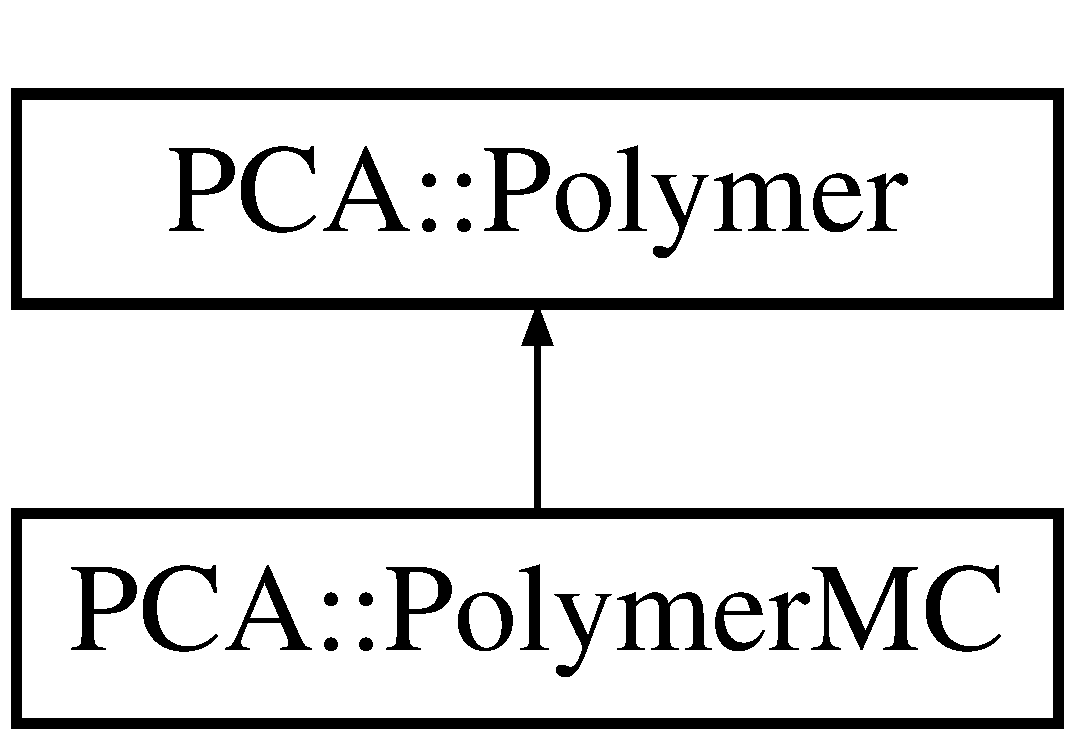
\includegraphics[height=2.000000cm]{class_p_c_a_1_1_polymer}
\end{center}
\end{figure}
\subsection*{Public Types}
\begin{DoxyCompactItemize}
\item 
enum \hyperlink{class_p_c_a_1_1_polymer_a1df36a764fbf04ccd5cbe8edb49d43bd}{File\+Type} \{ \hyperlink{class_p_c_a_1_1_polymer_a1df36a764fbf04ccd5cbe8edb49d43bda8387d77faaaa65484f5631d9f9d20bfc}{File\+Type\+::coordinates}, 
\hyperlink{class_p_c_a_1_1_polymer_a1df36a764fbf04ccd5cbe8edb49d43bda9bd139e0f52be4a748903ff60b5d3985}{File\+Type\+::angles}
 \}
\end{DoxyCompactItemize}
\subsection*{Public Member Functions}
\begin{DoxyCompactItemize}
\item 
\hyperlink{class_p_c_a_1_1_polymer_ac835d908dc32b787ca80f26cd0e6c68b}{Polymer} (\hyperlink{class_p_c_a_1_1_polymer_a1df36a764fbf04ccd5cbe8edb49d43bd}{File\+Type} file\+Type, char $\ast$file\+Name, int number\+Lines\+In\+Block=0, int polymer\+Number=1)
\begin{DoxyCompactList}\small\item\em Constructor\+: read coordinates of sites from file. \end{DoxyCompactList}\item 
\hyperlink{class_p_c_a_1_1_polymer_ac2645c33eba98a8ec1670d69b92060c8}{Polymer} (int number\+Of\+Monomers, const \hyperlink{class_p_c_a_1_1_vector}{Vector} $\ast$\hyperlink{class_p_c_a_1_1_polymer_a9822e3b9c3420a04a689706b84e586ca}{r}=N\+U\+LL, const \hyperlink{class_p_c_a_1_1_vector}{Vector} $\ast$\hyperlink{class_p_c_a_1_1_polymer_a0fd79e19a8c09a9e4c72903924151b5e}{t}=N\+U\+LL, const \hyperlink{class_p_c_a_1_1_vector}{Vector} $\ast$\hyperlink{class_p_c_a_1_1_polymer_ad93199b0187ab557476153b204b921c7}{b}=N\+U\+LL)
\begin{DoxyCompactList}\small\item\em Constructor. \end{DoxyCompactList}\item 
\hyperlink{class_p_c_a_1_1_polymer_a7d08722028cd9bf11b042a1b3b0e1d37}{Polymer} (int number\+Of\+Monomers, const double $\ast$kappa\+\_\+in, const double $\ast$tau\+\_\+in)
\begin{DoxyCompactList}\small\item\em Constructor. \end{DoxyCompactList}\item 
\hyperlink{class_p_c_a_1_1_polymer_a1ce99540db06e9e48392423ba516cd2f}{Polymer} (const \hyperlink{class_p_c_a_1_1_polymer}{Polymer} \&polymer)
\begin{DoxyCompactList}\small\item\em Copy constructor. \end{DoxyCompactList}\item 
\hyperlink{class_p_c_a_1_1_polymer_ac0d31fa5c6bee720f8069805d6669606}{$\sim$\+Polymer} ()
\begin{DoxyCompactList}\small\item\em Destructor. \end{DoxyCompactList}\item 
void \hyperlink{class_p_c_a_1_1_polymer_a55787461ed50776c48819a5cc3911c38}{set\+Vectors\+T\+N\+Bfrom\+Kappa\+Tau} ()
\begin{DoxyCompactList}\small\item\em Set vecors t(not unitary!) , n(unitary), b(unitary) and monomer\+Lengths. \end{DoxyCompactList}\item 
void \hyperlink{class_p_c_a_1_1_polymer_a0c6e93aa35271b98d92a38afd2b0913d}{set\+Radius\+Vector} (int i, double x\+\_\+in, double y\+\_\+in, double z\+\_\+in)
\item 
void \hyperlink{class_p_c_a_1_1_polymer_ac8631ac2842b00802f24478b525c05db}{set\+Kappa} (int i, double kappa\+\_\+in)
\item 
void \hyperlink{class_p_c_a_1_1_polymer_a4ac116507767651444c852a75ab79c2d}{set\+Tau} (int i, double tau\+\_\+in)
\item 
void \hyperlink{class_p_c_a_1_1_polymer_a9859e587476da47e49cfee1152e93fa0}{write\+Radius\+Vectors\+In\+File} (F\+I\+LE $\ast$fp) const
\item 
void \hyperlink{class_p_c_a_1_1_polymer_a081b8e4d7cac0da6cc411c7b56ff7362}{write\+Monomer\+Lengths\+In\+File} (F\+I\+LE $\ast$fp) const
\item 
void \hyperlink{class_p_c_a_1_1_polymer_ac89188a3e56684ff3313a43ff83abea0}{write\+T\+B\+Mfile} (char $\ast$file\+Name) const
\item 
double \hyperlink{class_p_c_a_1_1_polymer_a901d8c030d3edb333498edcc4502b27a}{distance} (int siteA, int siteB) const
\end{DoxyCompactItemize}
\begin{Indent}{\bf Set ones vectors from another vectors\+:}\par
\begin{DoxyCompactItemize}
\item 
void \hyperlink{class_p_c_a_1_1_polymer_aa655eb1299b272fef8c91f003abbf50d}{set\+Vectors\+Tfrom\+Radius\+Vectors} ()
\item 
void \hyperlink{class_p_c_a_1_1_polymer_a8dad939cbc8d8df73784526ad4a07aef}{set\+Vectors\+Bfrom\+VectorsT} ()
\item 
void \hyperlink{class_p_c_a_1_1_polymer_a258f607c38c1a247dd37659b236aa3fa}{set\+Radius\+Vectors\+From\+VectorsT} ()
\end{DoxyCompactItemize}
\end{Indent}
\begin{Indent}{\bf Set lengths of all monomers from vectors\+:}\par
\begin{DoxyCompactItemize}
\item 
void \hyperlink{class_p_c_a_1_1_polymer_a2dae638afa952c286c16122c7ab52b6e}{set\+Monomer\+Lengths\+From\+Radius\+Vectors} ()
\item 
void \hyperlink{class_p_c_a_1_1_polymer_a217cddfa5b9e5bfe68f8e5d0802e2f31}{set\+Monomer\+Lengths\+From\+VectorsT} ()
\end{DoxyCompactItemize}
\end{Indent}
\begin{Indent}{\bf Functions which returns members\+:}\par
\begin{DoxyCompactItemize}
\item 
int \hyperlink{class_p_c_a_1_1_polymer_a5c87b083f77c06ffd14278f87dad47ea}{get\+Num\+Monomers} () const
\item 
const double $\ast$ \hyperlink{class_p_c_a_1_1_polymer_af05e598bcd1e9987aca46d0661ac6dca}{get\+Monomer\+Length} () const
\item 
const \hyperlink{class_p_c_a_1_1_vector}{Vector} $\ast$ \hyperlink{class_p_c_a_1_1_polymer_a6e913f9b50a164c828f9a3cb89e452e1}{get\+Radius\+Vectors} () const
\item 
const \hyperlink{class_p_c_a_1_1_vector}{Vector} \& \hyperlink{class_p_c_a_1_1_polymer_ab2ea86763e0f0be646ef6aa6a105f927}{get\+Radius\+Vector} (int site) const
\item 
const \hyperlink{class_p_c_a_1_1_vector}{Vector} $\ast$ \hyperlink{class_p_c_a_1_1_polymer_a83c92fb07eafc88d121ef4b4124319c3}{get\+VectorsT} () const
\item 
const \hyperlink{class_p_c_a_1_1_vector}{Vector} $\ast$ \hyperlink{class_p_c_a_1_1_polymer_a4a90f901ceb688b0d96b126cc2ba3678}{get\+VectorsB} () const
\item 
double \hyperlink{class_p_c_a_1_1_polymer_ac0cafb89b662aaa3be2bbc7bf034d410}{get\+Kappa} (int i) const
\item 
double \hyperlink{class_p_c_a_1_1_polymer_a01b636d898a08113ca9bf556447934ec}{get\+Tau} (int i) const
\end{DoxyCompactItemize}
\end{Indent}
\subsection*{Protected Member Functions}
\begin{DoxyCompactItemize}
\item 
void \hyperlink{class_p_c_a_1_1_polymer_a777691bb321ef1da30a064757eb480c7}{read\+File\+With\+Coordinates} (char $\ast$file\+Name, int lines\+In\+Block, int block\+Number=1)
\begin{DoxyCompactList}\small\item\em Read file with x y z coordinates and fill r\mbox{[}\mbox{]}. \end{DoxyCompactList}\item 
void \hyperlink{class_p_c_a_1_1_polymer_a3e498b6e57d98c9cc4d07a7aedb4b6a5}{read\+File\+With\+Angles} (char $\ast$file\+Name, int lines\+In\+Block, int block\+Number=1)
\begin{DoxyCompactList}\small\item\em Read file with kappa tau angles and fill corresponding arrays. \end{DoxyCompactList}\item 
void \hyperlink{class_p_c_a_1_1_polymer_a3fcca4084a54ac8bc1941b36462bc560}{format\+All} ()
\begin{DoxyCompactList}\small\item\em The same as destructor. \end{DoxyCompactList}\end{DoxyCompactItemize}
\subsection*{Protected Attributes}
\begin{DoxyCompactItemize}
\item 
int \hyperlink{class_p_c_a_1_1_polymer_a8dadd2d6d6d65b79909f274acd63fd1e}{num\+Monomers}
\begin{DoxyCompactList}\small\item\em Number of monomers in polymer chain. \end{DoxyCompactList}\item 
double $\ast$ \hyperlink{class_p_c_a_1_1_polymer_adec33c5274834c85479abefe537efa5a}{monomer\+Length}
\begin{DoxyCompactList}\small\item\em monomer length \end{DoxyCompactList}\item 
\hyperlink{class_p_c_a_1_1_vector}{Vector} $\ast$ \hyperlink{class_p_c_a_1_1_polymer_a9822e3b9c3420a04a689706b84e586ca}{r}
\begin{DoxyCompactList}\small\item\em radius vectors \end{DoxyCompactList}\end{DoxyCompactItemize}
\begin{Indent}{\bf Frenet angles\+:}\par
\begin{DoxyCompactItemize}
\item 
double $\ast$ \hyperlink{class_p_c_a_1_1_polymer_a1bef29f1613bb4b67981aae7df3d804b}{kappa}
\begin{DoxyCompactList}\small\item\em bound angle \end{DoxyCompactList}\item 
double $\ast$ \hyperlink{class_p_c_a_1_1_polymer_ab3b07298bdbac01a7b20b2554d7b248f}{tau}
\begin{DoxyCompactList}\small\item\em torsion angle \end{DoxyCompactList}\end{DoxyCompactItemize}
\end{Indent}
\begin{Indent}{\bf Frenet frame vectors\+:}\par
\begin{DoxyCompactItemize}
\item 
\hyperlink{class_p_c_a_1_1_vector}{Vector} $\ast$ \hyperlink{class_p_c_a_1_1_polymer_a0fd79e19a8c09a9e4c72903924151b5e}{t}
\begin{DoxyCompactList}\small\item\em tangent not-\/unit vectors \end{DoxyCompactList}\item 
\hyperlink{class_p_c_a_1_1_vector}{Vector} $\ast$ \hyperlink{class_p_c_a_1_1_polymer_a7c71d8f5516ae0b0ead3929296135d1b}{n}
\begin{DoxyCompactList}\small\item\em normal unit vectors \end{DoxyCompactList}\item 
\hyperlink{class_p_c_a_1_1_vector}{Vector} $\ast$ \hyperlink{class_p_c_a_1_1_polymer_ad93199b0187ab557476153b204b921c7}{b}
\begin{DoxyCompactList}\small\item\em binormal unot vectors \end{DoxyCompactList}\end{DoxyCompactItemize}
\end{Indent}


\subsection{Member Enumeration Documentation}
\hypertarget{class_p_c_a_1_1_polymer_a1df36a764fbf04ccd5cbe8edb49d43bd}{}\label{class_p_c_a_1_1_polymer_a1df36a764fbf04ccd5cbe8edb49d43bd} 
\index{P\+C\+A\+::\+Polymer@{P\+C\+A\+::\+Polymer}!File\+Type@{File\+Type}}
\index{File\+Type@{File\+Type}!P\+C\+A\+::\+Polymer@{P\+C\+A\+::\+Polymer}}
\subsubsection{\texorpdfstring{File\+Type}{FileType}}
{\footnotesize\ttfamily enum \hyperlink{class_p_c_a_1_1_polymer_a1df36a764fbf04ccd5cbe8edb49d43bd}{P\+C\+A\+::\+Polymer\+::\+File\+Type}\hspace{0.3cm}{\ttfamily [strong]}}

\begin{DoxyEnumFields}{Enumerator}
\raisebox{\heightof{T}}[0pt][0pt]{\index{coordinates@{coordinates}!P\+C\+A\+::\+Polymer@{P\+C\+A\+::\+Polymer}}\index{P\+C\+A\+::\+Polymer@{P\+C\+A\+::\+Polymer}!coordinates@{coordinates}}}\hypertarget{class_p_c_a_1_1_polymer_a1df36a764fbf04ccd5cbe8edb49d43bda8387d77faaaa65484f5631d9f9d20bfc}{}\label{class_p_c_a_1_1_polymer_a1df36a764fbf04ccd5cbe8edb49d43bda8387d77faaaa65484f5631d9f9d20bfc} 
coordinates&\\
\hline

\raisebox{\heightof{T}}[0pt][0pt]{\index{angles@{angles}!P\+C\+A\+::\+Polymer@{P\+C\+A\+::\+Polymer}}\index{P\+C\+A\+::\+Polymer@{P\+C\+A\+::\+Polymer}!angles@{angles}}}\hypertarget{class_p_c_a_1_1_polymer_a1df36a764fbf04ccd5cbe8edb49d43bda9bd139e0f52be4a748903ff60b5d3985}{}\label{class_p_c_a_1_1_polymer_a1df36a764fbf04ccd5cbe8edb49d43bda9bd139e0f52be4a748903ff60b5d3985} 
angles&\\
\hline

\end{DoxyEnumFields}


\subsection{Constructor \& Destructor Documentation}
\hypertarget{class_p_c_a_1_1_polymer_ac835d908dc32b787ca80f26cd0e6c68b}{}\label{class_p_c_a_1_1_polymer_ac835d908dc32b787ca80f26cd0e6c68b} 
\index{P\+C\+A\+::\+Polymer@{P\+C\+A\+::\+Polymer}!Polymer@{Polymer}}
\index{Polymer@{Polymer}!P\+C\+A\+::\+Polymer@{P\+C\+A\+::\+Polymer}}
\subsubsection{\texorpdfstring{Polymer()}{Polymer()}\hspace{0.1cm}{\footnotesize\ttfamily [1/4]}}
{\footnotesize\ttfamily P\+C\+A\+::\+Polymer\+::\+Polymer (\begin{DoxyParamCaption}\item[{\hyperlink{class_p_c_a_1_1_polymer_a1df36a764fbf04ccd5cbe8edb49d43bd}{File\+Type}}]{file\+Type,  }\item[{char $\ast$}]{file\+Name,  }\item[{int}]{number\+Lines\+In\+Block = {\ttfamily 0},  }\item[{int}]{polymer\+Number = {\ttfamily 1} }\end{DoxyParamCaption})}



Constructor\+: read coordinates of sites from file. 

If you have more than one blocks in file then pass the number of the block. You can pass number of sites in the block, but it is not necessarily. \hypertarget{class_p_c_a_1_1_polymer_ac2645c33eba98a8ec1670d69b92060c8}{}\label{class_p_c_a_1_1_polymer_ac2645c33eba98a8ec1670d69b92060c8} 
\index{P\+C\+A\+::\+Polymer@{P\+C\+A\+::\+Polymer}!Polymer@{Polymer}}
\index{Polymer@{Polymer}!P\+C\+A\+::\+Polymer@{P\+C\+A\+::\+Polymer}}
\subsubsection{\texorpdfstring{Polymer()}{Polymer()}\hspace{0.1cm}{\footnotesize\ttfamily [2/4]}}
{\footnotesize\ttfamily P\+C\+A\+::\+Polymer\+::\+Polymer (\begin{DoxyParamCaption}\item[{int}]{number\+Of\+Monomers,  }\item[{const \hyperlink{class_p_c_a_1_1_vector}{Vector} $\ast$}]{r = {\ttfamily NULL},  }\item[{const \hyperlink{class_p_c_a_1_1_vector}{Vector} $\ast$}]{t = {\ttfamily NULL},  }\item[{const \hyperlink{class_p_c_a_1_1_vector}{Vector} $\ast$}]{b = {\ttfamily NULL} }\end{DoxyParamCaption})}



Constructor. 

\hypertarget{class_p_c_a_1_1_polymer_a7d08722028cd9bf11b042a1b3b0e1d37}{}\label{class_p_c_a_1_1_polymer_a7d08722028cd9bf11b042a1b3b0e1d37} 
\index{P\+C\+A\+::\+Polymer@{P\+C\+A\+::\+Polymer}!Polymer@{Polymer}}
\index{Polymer@{Polymer}!P\+C\+A\+::\+Polymer@{P\+C\+A\+::\+Polymer}}
\subsubsection{\texorpdfstring{Polymer()}{Polymer()}\hspace{0.1cm}{\footnotesize\ttfamily [3/4]}}
{\footnotesize\ttfamily P\+C\+A\+::\+Polymer\+::\+Polymer (\begin{DoxyParamCaption}\item[{int}]{number\+Of\+Monomers,  }\item[{const double $\ast$}]{kappa\+\_\+in,  }\item[{const double $\ast$}]{tau\+\_\+in }\end{DoxyParamCaption})}



Constructor. 

\hypertarget{class_p_c_a_1_1_polymer_a1ce99540db06e9e48392423ba516cd2f}{}\label{class_p_c_a_1_1_polymer_a1ce99540db06e9e48392423ba516cd2f} 
\index{P\+C\+A\+::\+Polymer@{P\+C\+A\+::\+Polymer}!Polymer@{Polymer}}
\index{Polymer@{Polymer}!P\+C\+A\+::\+Polymer@{P\+C\+A\+::\+Polymer}}
\subsubsection{\texorpdfstring{Polymer()}{Polymer()}\hspace{0.1cm}{\footnotesize\ttfamily [4/4]}}
{\footnotesize\ttfamily P\+C\+A\+::\+Polymer\+::\+Polymer (\begin{DoxyParamCaption}\item[{const \hyperlink{class_p_c_a_1_1_polymer}{Polymer} \&}]{polymer }\end{DoxyParamCaption})}



Copy constructor. 

\hypertarget{class_p_c_a_1_1_polymer_ac0d31fa5c6bee720f8069805d6669606}{}\label{class_p_c_a_1_1_polymer_ac0d31fa5c6bee720f8069805d6669606} 
\index{P\+C\+A\+::\+Polymer@{P\+C\+A\+::\+Polymer}!````~Polymer@{$\sim$\+Polymer}}
\index{````~Polymer@{$\sim$\+Polymer}!P\+C\+A\+::\+Polymer@{P\+C\+A\+::\+Polymer}}
\subsubsection{\texorpdfstring{$\sim$\+Polymer()}{~Polymer()}}
{\footnotesize\ttfamily P\+C\+A\+::\+Polymer\+::$\sim$\+Polymer (\begin{DoxyParamCaption}{ }\end{DoxyParamCaption})}



Destructor. 



\subsection{Member Function Documentation}
\hypertarget{class_p_c_a_1_1_polymer_a901d8c030d3edb333498edcc4502b27a}{}\label{class_p_c_a_1_1_polymer_a901d8c030d3edb333498edcc4502b27a} 
\index{P\+C\+A\+::\+Polymer@{P\+C\+A\+::\+Polymer}!distance@{distance}}
\index{distance@{distance}!P\+C\+A\+::\+Polymer@{P\+C\+A\+::\+Polymer}}
\subsubsection{\texorpdfstring{distance()}{distance()}}
{\footnotesize\ttfamily double P\+C\+A\+::\+Polymer\+::distance (\begin{DoxyParamCaption}\item[{int}]{siteA,  }\item[{int}]{siteB }\end{DoxyParamCaption}) const}

\hypertarget{class_p_c_a_1_1_polymer_a3fcca4084a54ac8bc1941b36462bc560}{}\label{class_p_c_a_1_1_polymer_a3fcca4084a54ac8bc1941b36462bc560} 
\index{P\+C\+A\+::\+Polymer@{P\+C\+A\+::\+Polymer}!format\+All@{format\+All}}
\index{format\+All@{format\+All}!P\+C\+A\+::\+Polymer@{P\+C\+A\+::\+Polymer}}
\subsubsection{\texorpdfstring{format\+All()}{formatAll()}}
{\footnotesize\ttfamily void P\+C\+A\+::\+Polymer\+::format\+All (\begin{DoxyParamCaption}{ }\end{DoxyParamCaption})\hspace{0.3cm}{\ttfamily [protected]}}



The same as destructor. 

\hypertarget{class_p_c_a_1_1_polymer_ac0cafb89b662aaa3be2bbc7bf034d410}{}\label{class_p_c_a_1_1_polymer_ac0cafb89b662aaa3be2bbc7bf034d410} 
\index{P\+C\+A\+::\+Polymer@{P\+C\+A\+::\+Polymer}!get\+Kappa@{get\+Kappa}}
\index{get\+Kappa@{get\+Kappa}!P\+C\+A\+::\+Polymer@{P\+C\+A\+::\+Polymer}}
\subsubsection{\texorpdfstring{get\+Kappa()}{getKappa()}}
{\footnotesize\ttfamily double P\+C\+A\+::\+Polymer\+::get\+Kappa (\begin{DoxyParamCaption}\item[{int}]{i }\end{DoxyParamCaption}) const\hspace{0.3cm}{\ttfamily [inline]}}

\hypertarget{class_p_c_a_1_1_polymer_af05e598bcd1e9987aca46d0661ac6dca}{}\label{class_p_c_a_1_1_polymer_af05e598bcd1e9987aca46d0661ac6dca} 
\index{P\+C\+A\+::\+Polymer@{P\+C\+A\+::\+Polymer}!get\+Monomer\+Length@{get\+Monomer\+Length}}
\index{get\+Monomer\+Length@{get\+Monomer\+Length}!P\+C\+A\+::\+Polymer@{P\+C\+A\+::\+Polymer}}
\subsubsection{\texorpdfstring{get\+Monomer\+Length()}{getMonomerLength()}}
{\footnotesize\ttfamily const double $\ast$ P\+C\+A\+::\+Polymer\+::get\+Monomer\+Length (\begin{DoxyParamCaption}{ }\end{DoxyParamCaption}) const}

\hypertarget{class_p_c_a_1_1_polymer_a5c87b083f77c06ffd14278f87dad47ea}{}\label{class_p_c_a_1_1_polymer_a5c87b083f77c06ffd14278f87dad47ea} 
\index{P\+C\+A\+::\+Polymer@{P\+C\+A\+::\+Polymer}!get\+Num\+Monomers@{get\+Num\+Monomers}}
\index{get\+Num\+Monomers@{get\+Num\+Monomers}!P\+C\+A\+::\+Polymer@{P\+C\+A\+::\+Polymer}}
\subsubsection{\texorpdfstring{get\+Num\+Monomers()}{getNumMonomers()}}
{\footnotesize\ttfamily int P\+C\+A\+::\+Polymer\+::get\+Num\+Monomers (\begin{DoxyParamCaption}{ }\end{DoxyParamCaption}) const\hspace{0.3cm}{\ttfamily [inline]}}

\hypertarget{class_p_c_a_1_1_polymer_ab2ea86763e0f0be646ef6aa6a105f927}{}\label{class_p_c_a_1_1_polymer_ab2ea86763e0f0be646ef6aa6a105f927} 
\index{P\+C\+A\+::\+Polymer@{P\+C\+A\+::\+Polymer}!get\+Radius\+Vector@{get\+Radius\+Vector}}
\index{get\+Radius\+Vector@{get\+Radius\+Vector}!P\+C\+A\+::\+Polymer@{P\+C\+A\+::\+Polymer}}
\subsubsection{\texorpdfstring{get\+Radius\+Vector()}{getRadiusVector()}}
{\footnotesize\ttfamily const \hyperlink{class_p_c_a_1_1_vector}{Vector} \& P\+C\+A\+::\+Polymer\+::get\+Radius\+Vector (\begin{DoxyParamCaption}\item[{int}]{site }\end{DoxyParamCaption}) const}

\hypertarget{class_p_c_a_1_1_polymer_a6e913f9b50a164c828f9a3cb89e452e1}{}\label{class_p_c_a_1_1_polymer_a6e913f9b50a164c828f9a3cb89e452e1} 
\index{P\+C\+A\+::\+Polymer@{P\+C\+A\+::\+Polymer}!get\+Radius\+Vectors@{get\+Radius\+Vectors}}
\index{get\+Radius\+Vectors@{get\+Radius\+Vectors}!P\+C\+A\+::\+Polymer@{P\+C\+A\+::\+Polymer}}
\subsubsection{\texorpdfstring{get\+Radius\+Vectors()}{getRadiusVectors()}}
{\footnotesize\ttfamily const \hyperlink{class_p_c_a_1_1_vector}{Vector} $\ast$ P\+C\+A\+::\+Polymer\+::get\+Radius\+Vectors (\begin{DoxyParamCaption}{ }\end{DoxyParamCaption}) const}

\hypertarget{class_p_c_a_1_1_polymer_a01b636d898a08113ca9bf556447934ec}{}\label{class_p_c_a_1_1_polymer_a01b636d898a08113ca9bf556447934ec} 
\index{P\+C\+A\+::\+Polymer@{P\+C\+A\+::\+Polymer}!get\+Tau@{get\+Tau}}
\index{get\+Tau@{get\+Tau}!P\+C\+A\+::\+Polymer@{P\+C\+A\+::\+Polymer}}
\subsubsection{\texorpdfstring{get\+Tau()}{getTau()}}
{\footnotesize\ttfamily double P\+C\+A\+::\+Polymer\+::get\+Tau (\begin{DoxyParamCaption}\item[{int}]{i }\end{DoxyParamCaption}) const\hspace{0.3cm}{\ttfamily [inline]}}

\hypertarget{class_p_c_a_1_1_polymer_a4a90f901ceb688b0d96b126cc2ba3678}{}\label{class_p_c_a_1_1_polymer_a4a90f901ceb688b0d96b126cc2ba3678} 
\index{P\+C\+A\+::\+Polymer@{P\+C\+A\+::\+Polymer}!get\+VectorsB@{get\+VectorsB}}
\index{get\+VectorsB@{get\+VectorsB}!P\+C\+A\+::\+Polymer@{P\+C\+A\+::\+Polymer}}
\subsubsection{\texorpdfstring{get\+Vectors\+B()}{getVectorsB()}}
{\footnotesize\ttfamily const \hyperlink{class_p_c_a_1_1_vector}{Vector} $\ast$ P\+C\+A\+::\+Polymer\+::get\+VectorsB (\begin{DoxyParamCaption}{ }\end{DoxyParamCaption}) const}

\hypertarget{class_p_c_a_1_1_polymer_a83c92fb07eafc88d121ef4b4124319c3}{}\label{class_p_c_a_1_1_polymer_a83c92fb07eafc88d121ef4b4124319c3} 
\index{P\+C\+A\+::\+Polymer@{P\+C\+A\+::\+Polymer}!get\+VectorsT@{get\+VectorsT}}
\index{get\+VectorsT@{get\+VectorsT}!P\+C\+A\+::\+Polymer@{P\+C\+A\+::\+Polymer}}
\subsubsection{\texorpdfstring{get\+Vectors\+T()}{getVectorsT()}}
{\footnotesize\ttfamily const \hyperlink{class_p_c_a_1_1_vector}{Vector} $\ast$ P\+C\+A\+::\+Polymer\+::get\+VectorsT (\begin{DoxyParamCaption}{ }\end{DoxyParamCaption}) const}

\hypertarget{class_p_c_a_1_1_polymer_a3e498b6e57d98c9cc4d07a7aedb4b6a5}{}\label{class_p_c_a_1_1_polymer_a3e498b6e57d98c9cc4d07a7aedb4b6a5} 
\index{P\+C\+A\+::\+Polymer@{P\+C\+A\+::\+Polymer}!read\+File\+With\+Angles@{read\+File\+With\+Angles}}
\index{read\+File\+With\+Angles@{read\+File\+With\+Angles}!P\+C\+A\+::\+Polymer@{P\+C\+A\+::\+Polymer}}
\subsubsection{\texorpdfstring{read\+File\+With\+Angles()}{readFileWithAngles()}}
{\footnotesize\ttfamily void P\+C\+A\+::\+Polymer\+::read\+File\+With\+Angles (\begin{DoxyParamCaption}\item[{char $\ast$}]{file\+Name,  }\item[{int}]{lines\+In\+Block,  }\item[{int}]{block\+Number = {\ttfamily 1} }\end{DoxyParamCaption})\hspace{0.3cm}{\ttfamily [protected]}}



Read file with kappa tau angles and fill corresponding arrays. 

One line -\/ one atom. One block -\/ one chain. \hypertarget{class_p_c_a_1_1_polymer_a777691bb321ef1da30a064757eb480c7}{}\label{class_p_c_a_1_1_polymer_a777691bb321ef1da30a064757eb480c7} 
\index{P\+C\+A\+::\+Polymer@{P\+C\+A\+::\+Polymer}!read\+File\+With\+Coordinates@{read\+File\+With\+Coordinates}}
\index{read\+File\+With\+Coordinates@{read\+File\+With\+Coordinates}!P\+C\+A\+::\+Polymer@{P\+C\+A\+::\+Polymer}}
\subsubsection{\texorpdfstring{read\+File\+With\+Coordinates()}{readFileWithCoordinates()}}
{\footnotesize\ttfamily void P\+C\+A\+::\+Polymer\+::read\+File\+With\+Coordinates (\begin{DoxyParamCaption}\item[{char $\ast$}]{file\+Name,  }\item[{int}]{lines\+In\+Block,  }\item[{int}]{block\+Number = {\ttfamily 1} }\end{DoxyParamCaption})\hspace{0.3cm}{\ttfamily [protected]}}



Read file with x y z coordinates and fill r\mbox{[}\mbox{]}. 

One line -\/ one atom. One block -\/ one chain. Block is separated from another one with one or more empty lines. The first has number 1 (not 0).

N\+B1\+: in this version empty line is every line which starts with unprintable characters\+: \textbackslash{}n, \textbackslash{}t or space. That\textquotesingle{}s why any line with data can\textquotesingle{}t have unprintable character at the beginning.

N\+B2\+: You can\textquotesingle{}t have emty line before the first block. You don\textquotesingle{}t need to have empty line at the end of file. \hypertarget{class_p_c_a_1_1_polymer_ac8631ac2842b00802f24478b525c05db}{}\label{class_p_c_a_1_1_polymer_ac8631ac2842b00802f24478b525c05db} 
\index{P\+C\+A\+::\+Polymer@{P\+C\+A\+::\+Polymer}!set\+Kappa@{set\+Kappa}}
\index{set\+Kappa@{set\+Kappa}!P\+C\+A\+::\+Polymer@{P\+C\+A\+::\+Polymer}}
\subsubsection{\texorpdfstring{set\+Kappa()}{setKappa()}}
{\footnotesize\ttfamily void P\+C\+A\+::\+Polymer\+::set\+Kappa (\begin{DoxyParamCaption}\item[{int}]{i,  }\item[{double}]{kappa\+\_\+in }\end{DoxyParamCaption})\hspace{0.3cm}{\ttfamily [inline]}}

\hypertarget{class_p_c_a_1_1_polymer_a2dae638afa952c286c16122c7ab52b6e}{}\label{class_p_c_a_1_1_polymer_a2dae638afa952c286c16122c7ab52b6e} 
\index{P\+C\+A\+::\+Polymer@{P\+C\+A\+::\+Polymer}!set\+Monomer\+Lengths\+From\+Radius\+Vectors@{set\+Monomer\+Lengths\+From\+Radius\+Vectors}}
\index{set\+Monomer\+Lengths\+From\+Radius\+Vectors@{set\+Monomer\+Lengths\+From\+Radius\+Vectors}!P\+C\+A\+::\+Polymer@{P\+C\+A\+::\+Polymer}}
\subsubsection{\texorpdfstring{set\+Monomer\+Lengths\+From\+Radius\+Vectors()}{setMonomerLengthsFromRadiusVectors()}}
{\footnotesize\ttfamily void P\+C\+A\+::\+Polymer\+::set\+Monomer\+Lengths\+From\+Radius\+Vectors (\begin{DoxyParamCaption}{ }\end{DoxyParamCaption})}

\hypertarget{class_p_c_a_1_1_polymer_a217cddfa5b9e5bfe68f8e5d0802e2f31}{}\label{class_p_c_a_1_1_polymer_a217cddfa5b9e5bfe68f8e5d0802e2f31} 
\index{P\+C\+A\+::\+Polymer@{P\+C\+A\+::\+Polymer}!set\+Monomer\+Lengths\+From\+VectorsT@{set\+Monomer\+Lengths\+From\+VectorsT}}
\index{set\+Monomer\+Lengths\+From\+VectorsT@{set\+Monomer\+Lengths\+From\+VectorsT}!P\+C\+A\+::\+Polymer@{P\+C\+A\+::\+Polymer}}
\subsubsection{\texorpdfstring{set\+Monomer\+Lengths\+From\+Vectors\+T()}{setMonomerLengthsFromVectorsT()}}
{\footnotesize\ttfamily void P\+C\+A\+::\+Polymer\+::set\+Monomer\+Lengths\+From\+VectorsT (\begin{DoxyParamCaption}{ }\end{DoxyParamCaption})}

\hypertarget{class_p_c_a_1_1_polymer_a0c6e93aa35271b98d92a38afd2b0913d}{}\label{class_p_c_a_1_1_polymer_a0c6e93aa35271b98d92a38afd2b0913d} 
\index{P\+C\+A\+::\+Polymer@{P\+C\+A\+::\+Polymer}!set\+Radius\+Vector@{set\+Radius\+Vector}}
\index{set\+Radius\+Vector@{set\+Radius\+Vector}!P\+C\+A\+::\+Polymer@{P\+C\+A\+::\+Polymer}}
\subsubsection{\texorpdfstring{set\+Radius\+Vector()}{setRadiusVector()}}
{\footnotesize\ttfamily void P\+C\+A\+::\+Polymer\+::set\+Radius\+Vector (\begin{DoxyParamCaption}\item[{int}]{i,  }\item[{double}]{x\+\_\+in,  }\item[{double}]{y\+\_\+in,  }\item[{double}]{z\+\_\+in }\end{DoxyParamCaption})\hspace{0.3cm}{\ttfamily [inline]}}

\hypertarget{class_p_c_a_1_1_polymer_a258f607c38c1a247dd37659b236aa3fa}{}\label{class_p_c_a_1_1_polymer_a258f607c38c1a247dd37659b236aa3fa} 
\index{P\+C\+A\+::\+Polymer@{P\+C\+A\+::\+Polymer}!set\+Radius\+Vectors\+From\+VectorsT@{set\+Radius\+Vectors\+From\+VectorsT}}
\index{set\+Radius\+Vectors\+From\+VectorsT@{set\+Radius\+Vectors\+From\+VectorsT}!P\+C\+A\+::\+Polymer@{P\+C\+A\+::\+Polymer}}
\subsubsection{\texorpdfstring{set\+Radius\+Vectors\+From\+Vectors\+T()}{setRadiusVectorsFromVectorsT()}}
{\footnotesize\ttfamily void P\+C\+A\+::\+Polymer\+::set\+Radius\+Vectors\+From\+VectorsT (\begin{DoxyParamCaption}{ }\end{DoxyParamCaption})}

\hypertarget{class_p_c_a_1_1_polymer_a4ac116507767651444c852a75ab79c2d}{}\label{class_p_c_a_1_1_polymer_a4ac116507767651444c852a75ab79c2d} 
\index{P\+C\+A\+::\+Polymer@{P\+C\+A\+::\+Polymer}!set\+Tau@{set\+Tau}}
\index{set\+Tau@{set\+Tau}!P\+C\+A\+::\+Polymer@{P\+C\+A\+::\+Polymer}}
\subsubsection{\texorpdfstring{set\+Tau()}{setTau()}}
{\footnotesize\ttfamily void P\+C\+A\+::\+Polymer\+::set\+Tau (\begin{DoxyParamCaption}\item[{int}]{i,  }\item[{double}]{tau\+\_\+in }\end{DoxyParamCaption})\hspace{0.3cm}{\ttfamily [inline]}}

\hypertarget{class_p_c_a_1_1_polymer_a8dad939cbc8d8df73784526ad4a07aef}{}\label{class_p_c_a_1_1_polymer_a8dad939cbc8d8df73784526ad4a07aef} 
\index{P\+C\+A\+::\+Polymer@{P\+C\+A\+::\+Polymer}!set\+Vectors\+Bfrom\+VectorsT@{set\+Vectors\+Bfrom\+VectorsT}}
\index{set\+Vectors\+Bfrom\+VectorsT@{set\+Vectors\+Bfrom\+VectorsT}!P\+C\+A\+::\+Polymer@{P\+C\+A\+::\+Polymer}}
\subsubsection{\texorpdfstring{set\+Vectors\+Bfrom\+Vectors\+T()}{setVectorsBfromVectorsT()}}
{\footnotesize\ttfamily void P\+C\+A\+::\+Polymer\+::set\+Vectors\+Bfrom\+VectorsT (\begin{DoxyParamCaption}{ }\end{DoxyParamCaption})}

\hypertarget{class_p_c_a_1_1_polymer_aa655eb1299b272fef8c91f003abbf50d}{}\label{class_p_c_a_1_1_polymer_aa655eb1299b272fef8c91f003abbf50d} 
\index{P\+C\+A\+::\+Polymer@{P\+C\+A\+::\+Polymer}!set\+Vectors\+Tfrom\+Radius\+Vectors@{set\+Vectors\+Tfrom\+Radius\+Vectors}}
\index{set\+Vectors\+Tfrom\+Radius\+Vectors@{set\+Vectors\+Tfrom\+Radius\+Vectors}!P\+C\+A\+::\+Polymer@{P\+C\+A\+::\+Polymer}}
\subsubsection{\texorpdfstring{set\+Vectors\+Tfrom\+Radius\+Vectors()}{setVectorsTfromRadiusVectors()}}
{\footnotesize\ttfamily void P\+C\+A\+::\+Polymer\+::set\+Vectors\+Tfrom\+Radius\+Vectors (\begin{DoxyParamCaption}{ }\end{DoxyParamCaption})}

\hypertarget{class_p_c_a_1_1_polymer_a55787461ed50776c48819a5cc3911c38}{}\label{class_p_c_a_1_1_polymer_a55787461ed50776c48819a5cc3911c38} 
\index{P\+C\+A\+::\+Polymer@{P\+C\+A\+::\+Polymer}!set\+Vectors\+T\+N\+Bfrom\+Kappa\+Tau@{set\+Vectors\+T\+N\+Bfrom\+Kappa\+Tau}}
\index{set\+Vectors\+T\+N\+Bfrom\+Kappa\+Tau@{set\+Vectors\+T\+N\+Bfrom\+Kappa\+Tau}!P\+C\+A\+::\+Polymer@{P\+C\+A\+::\+Polymer}}
\subsubsection{\texorpdfstring{set\+Vectors\+T\+N\+Bfrom\+Kappa\+Tau()}{setVectorsTNBfromKappaTau()}}
{\footnotesize\ttfamily void P\+C\+A\+::\+Polymer\+::set\+Vectors\+T\+N\+Bfrom\+Kappa\+Tau (\begin{DoxyParamCaption}{ }\end{DoxyParamCaption})}



Set vecors t(not unitary!) , n(unitary), b(unitary) and monomer\+Lengths. 

\hypertarget{class_p_c_a_1_1_polymer_a081b8e4d7cac0da6cc411c7b56ff7362}{}\label{class_p_c_a_1_1_polymer_a081b8e4d7cac0da6cc411c7b56ff7362} 
\index{P\+C\+A\+::\+Polymer@{P\+C\+A\+::\+Polymer}!write\+Monomer\+Lengths\+In\+File@{write\+Monomer\+Lengths\+In\+File}}
\index{write\+Monomer\+Lengths\+In\+File@{write\+Monomer\+Lengths\+In\+File}!P\+C\+A\+::\+Polymer@{P\+C\+A\+::\+Polymer}}
\subsubsection{\texorpdfstring{write\+Monomer\+Lengths\+In\+File()}{writeMonomerLengthsInFile()}}
{\footnotesize\ttfamily void P\+C\+A\+::\+Polymer\+::write\+Monomer\+Lengths\+In\+File (\begin{DoxyParamCaption}\item[{F\+I\+LE $\ast$}]{fp }\end{DoxyParamCaption}) const}

\hypertarget{class_p_c_a_1_1_polymer_a9859e587476da47e49cfee1152e93fa0}{}\label{class_p_c_a_1_1_polymer_a9859e587476da47e49cfee1152e93fa0} 
\index{P\+C\+A\+::\+Polymer@{P\+C\+A\+::\+Polymer}!write\+Radius\+Vectors\+In\+File@{write\+Radius\+Vectors\+In\+File}}
\index{write\+Radius\+Vectors\+In\+File@{write\+Radius\+Vectors\+In\+File}!P\+C\+A\+::\+Polymer@{P\+C\+A\+::\+Polymer}}
\subsubsection{\texorpdfstring{write\+Radius\+Vectors\+In\+File()}{writeRadiusVectorsInFile()}}
{\footnotesize\ttfamily void P\+C\+A\+::\+Polymer\+::write\+Radius\+Vectors\+In\+File (\begin{DoxyParamCaption}\item[{F\+I\+LE $\ast$}]{fp }\end{DoxyParamCaption}) const}

\hypertarget{class_p_c_a_1_1_polymer_ac89188a3e56684ff3313a43ff83abea0}{}\label{class_p_c_a_1_1_polymer_ac89188a3e56684ff3313a43ff83abea0} 
\index{P\+C\+A\+::\+Polymer@{P\+C\+A\+::\+Polymer}!write\+T\+B\+Mfile@{write\+T\+B\+Mfile}}
\index{write\+T\+B\+Mfile@{write\+T\+B\+Mfile}!P\+C\+A\+::\+Polymer@{P\+C\+A\+::\+Polymer}}
\subsubsection{\texorpdfstring{write\+T\+B\+Mfile()}{writeTBMfile()}}
{\footnotesize\ttfamily void P\+C\+A\+::\+Polymer\+::write\+T\+B\+Mfile (\begin{DoxyParamCaption}\item[{char $\ast$}]{file\+Name }\end{DoxyParamCaption}) const}



\subsection{Member Data Documentation}
\hypertarget{class_p_c_a_1_1_polymer_ad93199b0187ab557476153b204b921c7}{}\label{class_p_c_a_1_1_polymer_ad93199b0187ab557476153b204b921c7} 
\index{P\+C\+A\+::\+Polymer@{P\+C\+A\+::\+Polymer}!b@{b}}
\index{b@{b}!P\+C\+A\+::\+Polymer@{P\+C\+A\+::\+Polymer}}
\subsubsection{\texorpdfstring{b}{b}}
{\footnotesize\ttfamily \hyperlink{class_p_c_a_1_1_vector}{Vector}$\ast$ P\+C\+A\+::\+Polymer\+::b\hspace{0.3cm}{\ttfamily [protected]}}



binormal unot vectors 

\hypertarget{class_p_c_a_1_1_polymer_a1bef29f1613bb4b67981aae7df3d804b}{}\label{class_p_c_a_1_1_polymer_a1bef29f1613bb4b67981aae7df3d804b} 
\index{P\+C\+A\+::\+Polymer@{P\+C\+A\+::\+Polymer}!kappa@{kappa}}
\index{kappa@{kappa}!P\+C\+A\+::\+Polymer@{P\+C\+A\+::\+Polymer}}
\subsubsection{\texorpdfstring{kappa}{kappa}}
{\footnotesize\ttfamily double$\ast$ P\+C\+A\+::\+Polymer\+::kappa\hspace{0.3cm}{\ttfamily [protected]}}



bound angle 

\hypertarget{class_p_c_a_1_1_polymer_adec33c5274834c85479abefe537efa5a}{}\label{class_p_c_a_1_1_polymer_adec33c5274834c85479abefe537efa5a} 
\index{P\+C\+A\+::\+Polymer@{P\+C\+A\+::\+Polymer}!monomer\+Length@{monomer\+Length}}
\index{monomer\+Length@{monomer\+Length}!P\+C\+A\+::\+Polymer@{P\+C\+A\+::\+Polymer}}
\subsubsection{\texorpdfstring{monomer\+Length}{monomerLength}}
{\footnotesize\ttfamily double$\ast$ P\+C\+A\+::\+Polymer\+::monomer\+Length\hspace{0.3cm}{\ttfamily [protected]}}



monomer length 

\hypertarget{class_p_c_a_1_1_polymer_a7c71d8f5516ae0b0ead3929296135d1b}{}\label{class_p_c_a_1_1_polymer_a7c71d8f5516ae0b0ead3929296135d1b} 
\index{P\+C\+A\+::\+Polymer@{P\+C\+A\+::\+Polymer}!n@{n}}
\index{n@{n}!P\+C\+A\+::\+Polymer@{P\+C\+A\+::\+Polymer}}
\subsubsection{\texorpdfstring{n}{n}}
{\footnotesize\ttfamily \hyperlink{class_p_c_a_1_1_vector}{Vector}$\ast$ P\+C\+A\+::\+Polymer\+::n\hspace{0.3cm}{\ttfamily [protected]}}



normal unit vectors 

\hypertarget{class_p_c_a_1_1_polymer_a8dadd2d6d6d65b79909f274acd63fd1e}{}\label{class_p_c_a_1_1_polymer_a8dadd2d6d6d65b79909f274acd63fd1e} 
\index{P\+C\+A\+::\+Polymer@{P\+C\+A\+::\+Polymer}!num\+Monomers@{num\+Monomers}}
\index{num\+Monomers@{num\+Monomers}!P\+C\+A\+::\+Polymer@{P\+C\+A\+::\+Polymer}}
\subsubsection{\texorpdfstring{num\+Monomers}{numMonomers}}
{\footnotesize\ttfamily int P\+C\+A\+::\+Polymer\+::num\+Monomers\hspace{0.3cm}{\ttfamily [protected]}}



Number of monomers in polymer chain. 

\hypertarget{class_p_c_a_1_1_polymer_a9822e3b9c3420a04a689706b84e586ca}{}\label{class_p_c_a_1_1_polymer_a9822e3b9c3420a04a689706b84e586ca} 
\index{P\+C\+A\+::\+Polymer@{P\+C\+A\+::\+Polymer}!r@{r}}
\index{r@{r}!P\+C\+A\+::\+Polymer@{P\+C\+A\+::\+Polymer}}
\subsubsection{\texorpdfstring{r}{r}}
{\footnotesize\ttfamily \hyperlink{class_p_c_a_1_1_vector}{Vector}$\ast$ P\+C\+A\+::\+Polymer\+::r\hspace{0.3cm}{\ttfamily [protected]}}



radius vectors 

\hypertarget{class_p_c_a_1_1_polymer_a0fd79e19a8c09a9e4c72903924151b5e}{}\label{class_p_c_a_1_1_polymer_a0fd79e19a8c09a9e4c72903924151b5e} 
\index{P\+C\+A\+::\+Polymer@{P\+C\+A\+::\+Polymer}!t@{t}}
\index{t@{t}!P\+C\+A\+::\+Polymer@{P\+C\+A\+::\+Polymer}}
\subsubsection{\texorpdfstring{t}{t}}
{\footnotesize\ttfamily \hyperlink{class_p_c_a_1_1_vector}{Vector}$\ast$ P\+C\+A\+::\+Polymer\+::t\hspace{0.3cm}{\ttfamily [protected]}}



tangent not-\/unit vectors 

\hypertarget{class_p_c_a_1_1_polymer_ab3b07298bdbac01a7b20b2554d7b248f}{}\label{class_p_c_a_1_1_polymer_ab3b07298bdbac01a7b20b2554d7b248f} 
\index{P\+C\+A\+::\+Polymer@{P\+C\+A\+::\+Polymer}!tau@{tau}}
\index{tau@{tau}!P\+C\+A\+::\+Polymer@{P\+C\+A\+::\+Polymer}}
\subsubsection{\texorpdfstring{tau}{tau}}
{\footnotesize\ttfamily double$\ast$ P\+C\+A\+::\+Polymer\+::tau\hspace{0.3cm}{\ttfamily [protected]}}



torsion angle 



The documentation for this class was generated from the following files\+:\begin{DoxyCompactItemize}
\item 
/\+Users/annsi118/\+Documents/\+Git\+\_\+projects/\+P\+C\+M\+C/include/\hyperlink{_polymer_8h}{Polymer.\+h}\item 
/\+Users/annsi118/\+Documents/\+Git\+\_\+projects/\+P\+C\+M\+C/source/\hyperlink{_polymer_8cpp}{Polymer.\+cpp}\end{DoxyCompactItemize}

\hypertarget{class_p_c_a_1_1_polymer_energy}{}\section{P\+CA\+:\+:Polymer\+Energy Class Reference}
\label{class_p_c_a_1_1_polymer_energy}\index{P\+C\+A\+::\+Polymer\+Energy@{P\+C\+A\+::\+Polymer\+Energy}}


{\ttfamily \#include $<$Polymer\+Energy.\+h$>$}

\subsection*{Classes}
\begin{DoxyCompactItemize}
\item 
class \hyperlink{class_p_c_a_1_1_polymer_energy_1_1_d_wparam}{D\+Wparam}
\begin{DoxyCompactList}\small\item\em Parameters for double-\/well potential. \end{DoxyCompactList}\item 
class \hyperlink{class_p_c_a_1_1_polymer_energy_1_1_l_jparam}{L\+Jparam}
\begin{DoxyCompactList}\small\item\em Parameters for Lennard-\/\+Jones potential. \end{DoxyCompactList}\end{DoxyCompactItemize}
\subsection*{Static Public Member Functions}
\begin{DoxyCompactItemize}
\item 
static double \hyperlink{class_p_c_a_1_1_polymer_energy_a835b345f0e6151a18962e4fb06a922bf}{site\+D\+Wenergy} (int site, int num\+Sites, const \hyperlink{class_p_c_a_1_1_polymer_energy_1_1_d_wparam}{D\+Wparam} \&param)
\item 
static double \hyperlink{class_p_c_a_1_1_polymer_energy_af55384a44f3e1aa5f32788b179d1cfe8}{full\+D\+Wenergy} (int num\+Sites, const \hyperlink{class_p_c_a_1_1_polymer_energy_1_1_d_wparam}{D\+Wparam} \&param)
\end{DoxyCompactItemize}


\subsection{Member Function Documentation}
\hypertarget{class_p_c_a_1_1_polymer_energy_af55384a44f3e1aa5f32788b179d1cfe8}{}\label{class_p_c_a_1_1_polymer_energy_af55384a44f3e1aa5f32788b179d1cfe8} 
\index{P\+C\+A\+::\+Polymer\+Energy@{P\+C\+A\+::\+Polymer\+Energy}!full\+D\+Wenergy@{full\+D\+Wenergy}}
\index{full\+D\+Wenergy@{full\+D\+Wenergy}!P\+C\+A\+::\+Polymer\+Energy@{P\+C\+A\+::\+Polymer\+Energy}}
\subsubsection{\texorpdfstring{full\+D\+Wenergy()}{fullDWenergy()}}
{\footnotesize\ttfamily static double P\+C\+A\+::\+Polymer\+Energy\+::full\+D\+Wenergy (\begin{DoxyParamCaption}\item[{int}]{num\+Sites,  }\item[{const \hyperlink{class_p_c_a_1_1_polymer_energy_1_1_d_wparam}{D\+Wparam} \&}]{param }\end{DoxyParamCaption})\hspace{0.3cm}{\ttfamily [static]}}

\hypertarget{class_p_c_a_1_1_polymer_energy_a835b345f0e6151a18962e4fb06a922bf}{}\label{class_p_c_a_1_1_polymer_energy_a835b345f0e6151a18962e4fb06a922bf} 
\index{P\+C\+A\+::\+Polymer\+Energy@{P\+C\+A\+::\+Polymer\+Energy}!site\+D\+Wenergy@{site\+D\+Wenergy}}
\index{site\+D\+Wenergy@{site\+D\+Wenergy}!P\+C\+A\+::\+Polymer\+Energy@{P\+C\+A\+::\+Polymer\+Energy}}
\subsubsection{\texorpdfstring{site\+D\+Wenergy()}{siteDWenergy()}}
{\footnotesize\ttfamily double P\+C\+A\+::\+Polymer\+Energy\+::site\+D\+Wenergy (\begin{DoxyParamCaption}\item[{int}]{site,  }\item[{int}]{num\+Sites,  }\item[{const \hyperlink{class_p_c_a_1_1_polymer_energy_1_1_d_wparam}{D\+Wparam} \&}]{param }\end{DoxyParamCaption})\hspace{0.3cm}{\ttfamily [static]}}



The documentation for this class was generated from the following files\+:\begin{DoxyCompactItemize}
\item 
/\+Users/annsi118/\+Documents/\+Git\+\_\+projects/\+P\+C\+M\+C/\+Temporary/\hyperlink{_polymer_energy_8h}{Polymer\+Energy.\+h}\item 
/\+Users/annsi118/\+Documents/\+Git\+\_\+projects/\+P\+C\+M\+C/\+Temporary/\hyperlink{_polymer_energy_8cpp}{Polymer\+Energy.\+cpp}\end{DoxyCompactItemize}

\hypertarget{class_p_c_a_1_1_polymer_m_c}{}\section{P\+CA\+:\+:Polymer\+MC Class Reference}
\label{class_p_c_a_1_1_polymer_m_c}\index{P\+C\+A\+::\+Polymer\+MC@{P\+C\+A\+::\+Polymer\+MC}}


{\ttfamily \#include $<$Polymer\+M\+C.\+h$>$}

Inheritance diagram for P\+CA\+:\+:Polymer\+MC\+:\begin{figure}[H]
\begin{center}
\leavevmode
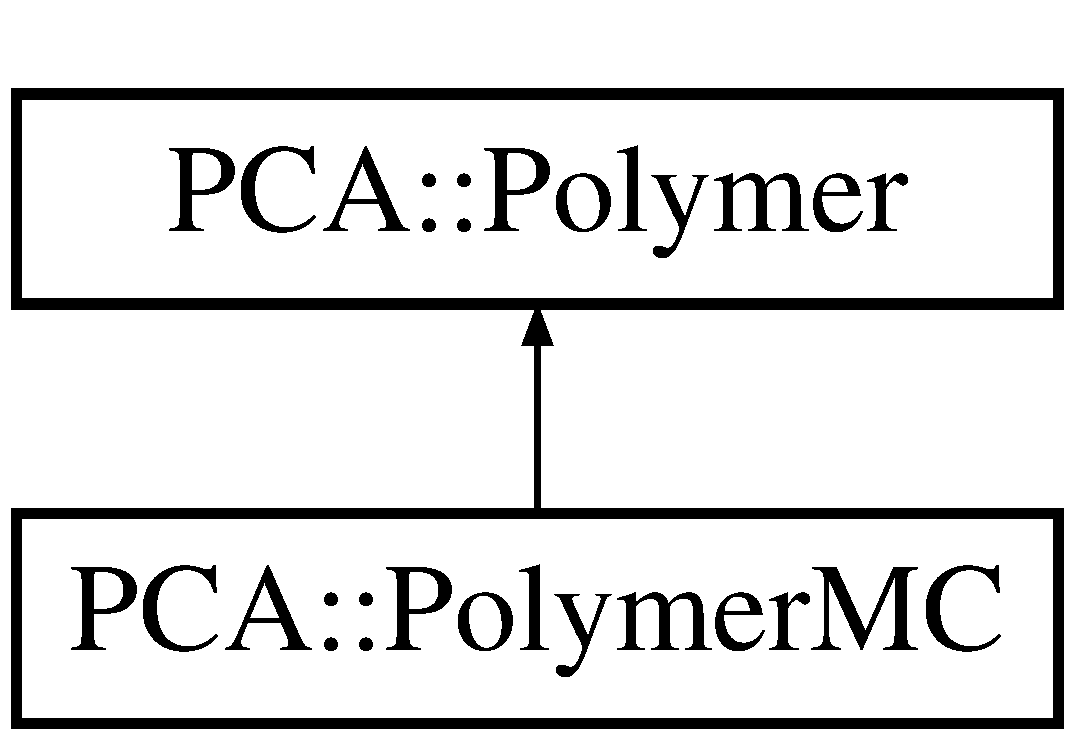
\includegraphics[height=2.000000cm]{class_p_c_a_1_1_polymer_m_c}
\end{center}
\end{figure}
\subsection*{Classes}
\begin{DoxyCompactItemize}
\item 
struct \hyperlink{struct_p_c_a_1_1_polymer_m_c_1_1_interaction_site}{Interaction\+Site}
\end{DoxyCompactItemize}
\subsection*{Public Member Functions}
\begin{DoxyCompactItemize}
\item 
\hyperlink{class_p_c_a_1_1_polymer_m_c_a0d90616fbc7d2eaaeedbdce0bc9057f0}{Polymer\+MC} (int number\+Of\+Monomers)
\begin{DoxyCompactList}\small\item\em Constructor. \end{DoxyCompactList}\item 
\hyperlink{class_p_c_a_1_1_polymer_m_c_a4617bc87ec890ae0817f2a1f20644611}{Polymer\+MC} (\hyperlink{class_p_c_a_1_1_polymer_a1df36a764fbf04ccd5cbe8edb49d43bd}{File\+Type} file\+Type, char $\ast$file\+Name, int number\+Lines\+In\+Block=0, int polymer\+Number=1)
\item 
\hyperlink{class_p_c_a_1_1_polymer_m_c_a6ed770992221cd0a7a9e364d4d5fcda3}{$\sim$\+Polymer\+MC} ()
\begin{DoxyCompactList}\small\item\em Destructor. \end{DoxyCompactList}\item 
void \hyperlink{class_p_c_a_1_1_polymer_m_c_ab075a6b6e2053461e15770d8db4f8917}{init\+With\+Random\+Taus} ()
\begin{DoxyCompactList}\small\item\em Initialization of \hyperlink{class_p_c_a_1_1_polymer_m_c}{Polymer\+MC} with random taus and kappas = 0. \end{DoxyCompactList}\item 
void \hyperlink{class_p_c_a_1_1_polymer_m_c_a327234bb757279e61f1b47ba493aaaa2}{init\+Test} ()
\begin{DoxyCompactList}\small\item\em Initialization of \hyperlink{class_p_c_a_1_1_polymer_m_c}{Polymer\+MC} for testing. \end{DoxyCompactList}\item 
void \hyperlink{class_p_c_a_1_1_polymer_m_c_a6e0c4626aff4270d9a1ece7fc51f3c0f}{save\+Old\+Radius\+Vectors} (int site)
\begin{DoxyCompactList}\small\item\em Saves old radius vectors starting from (site+1)\+: r\+Old\mbox{[}site+1\mbox{]}=r\mbox{[}site+1\mbox{]} ... \end{DoxyCompactList}\item 
void \hyperlink{class_p_c_a_1_1_polymer_m_c_a80c92a94292d085a0d0ce0563ae0a1fd}{set\+New\+Radius\+Vectors\+Via\+Rotation} (int site)
\begin{DoxyCompactList}\small\item\em This function changes only! r\mbox{[}site+1\mbox{]}, r\mbox{[}site+2\mbox{]}... \end{DoxyCompactList}\item 
void \hyperlink{class_p_c_a_1_1_polymer_m_c_ab7ec6ffe521bf27c218f4a6eac6c394b}{set\+New\+Vectors\+T\+N\+Bfrom\+Kappa\+Tau} (int site)
\begin{DoxyCompactList}\small\item\em Set t-\/ n-\/ b\mbox{[}i+1\mbox{]} and t-\/ n-\/ b\+New from kappa-\/ tau\mbox{[}i\mbox{]}. \end{DoxyCompactList}\item 
bool \hyperlink{class_p_c_a_1_1_polymer_m_c_a6f7e8a68070a688e1d6b0dc00a13b27c}{self\+Avoiding\+Condition} (double min\+Distance, int site)
\item 
void \hyperlink{class_p_c_a_1_1_polymer_m_c_aabe0e104c1f34ebe2174a650b7cbe963}{write\+Acceptence\+Rate\+In\+File} (F\+I\+LE $\ast$fp)
\end{DoxyCompactItemize}
\begin{Indent}{\bf Monte Carlo updates at kappa\mbox{[}site\mbox{]}/tau\mbox{[}site\mbox{]}}\par
\begin{DoxyCompactItemize}
\item 
void \hyperlink{class_p_c_a_1_1_polymer_m_c_a8d70317037e998d3a27618a9ecb60fd8}{kappa\+Update} (int site, double temperarture, const \hyperlink{class_p_c_a_1_1_hamiltonian}{Hamiltonian} \&hamiltonian, const \hyperlink{class_p_c_a_1_1_lennard_jones}{Lennard\+Jones} \&interaction)
\item 
void \hyperlink{class_p_c_a_1_1_polymer_m_c_a087b8392c8ec8eea5c069a1be4c46d2f}{tau\+Update} (int site, double temperarture, const \hyperlink{class_p_c_a_1_1_hamiltonian}{Hamiltonian} \&hamiltonian, const \hyperlink{class_p_c_a_1_1_lennard_jones}{Lennard\+Jones} \&interaction)
\item 
void \hyperlink{class_p_c_a_1_1_polymer_m_c_a4bb5653f7159bce31cc0e476b4fd4c8e}{update\+All\+Sites} (double temperature, const \hyperlink{class_p_c_a_1_1_hamiltonian}{Hamiltonian} \&hamiltonian, const \hyperlink{class_p_c_a_1_1_lennard_jones}{Lennard\+Jones} \&interaction)
\end{DoxyCompactItemize}
\end{Indent}
\subsection*{Private Attributes}
\begin{DoxyCompactItemize}
\item 
double \hyperlink{class_p_c_a_1_1_polymer_m_c_a6771be27571e5c106546eb5225edec05}{kappa\+New}
\item 
double \hyperlink{class_p_c_a_1_1_polymer_m_c_a6400a8ec5f791281122167837d6e4d7d}{tau\+New}
\item 
\hyperlink{class_p_c_a_1_1_vector}{Vector} $\ast$ \hyperlink{class_p_c_a_1_1_polymer_m_c_a6144923e16ec4e3086f92516d8a9117b}{r\+Old}
\item 
struct \hyperlink{struct_p_c_a_1_1_polymer_m_c_1_1_interaction_site}{P\+C\+A\+::\+Polymer\+M\+C\+::\+Interaction\+Site} \hyperlink{class_p_c_a_1_1_polymer_m_c_ac4bbb885c9b1953dd3bd2fbf1656822e}{interaction\+Site}
\item 
int \hyperlink{class_p_c_a_1_1_polymer_m_c_adc7d93c4f0f568dd5fd9b74064e0cd88}{accept\+Number\+Kappa}
\item 
int \hyperlink{class_p_c_a_1_1_polymer_m_c_a537709e4e856390abc7f511de2cf4c58}{accept\+Number\+Tau}
\item 
\hyperlink{class_p_c_a_1_1_uniform_rand}{Uniform\+Rand} \hyperlink{class_p_c_a_1_1_polymer_m_c_ac503a4c28f8c36289d34036ce1ebc0b2}{uni\+Rand}
\end{DoxyCompactItemize}
\begin{Indent}{\bf If kappa\+New corresponds to i site then t\+New correspondes to (i+1)}\par
\begin{DoxyCompactItemize}
\item 
\hyperlink{class_p_c_a_1_1_vector}{Vector} \hyperlink{class_p_c_a_1_1_polymer_m_c_a1220187032c23f9fd2d78886fd1815b3}{t\+New}
\item 
\hyperlink{class_p_c_a_1_1_vector}{Vector} \hyperlink{class_p_c_a_1_1_polymer_m_c_a5e493ca12a3eba2f1658ac1cccba3d56}{n\+New}
\item 
\hyperlink{class_p_c_a_1_1_vector}{Vector} \hyperlink{class_p_c_a_1_1_polymer_m_c_a69019643d3a1fd92b8c77647bb4a91d6}{b\+New}
\end{DoxyCompactItemize}
\end{Indent}
\subsection*{Additional Inherited Members}


\subsection{Constructor \& Destructor Documentation}
\hypertarget{class_p_c_a_1_1_polymer_m_c_a0d90616fbc7d2eaaeedbdce0bc9057f0}{}\label{class_p_c_a_1_1_polymer_m_c_a0d90616fbc7d2eaaeedbdce0bc9057f0} 
\index{P\+C\+A\+::\+Polymer\+MC@{P\+C\+A\+::\+Polymer\+MC}!Polymer\+MC@{Polymer\+MC}}
\index{Polymer\+MC@{Polymer\+MC}!P\+C\+A\+::\+Polymer\+MC@{P\+C\+A\+::\+Polymer\+MC}}
\subsubsection{\texorpdfstring{Polymer\+M\+C()}{PolymerMC()}\hspace{0.1cm}{\footnotesize\ttfamily [1/2]}}
{\footnotesize\ttfamily P\+C\+A\+::\+Polymer\+M\+C\+::\+Polymer\+MC (\begin{DoxyParamCaption}\item[{int}]{number\+Of\+Monomers }\end{DoxyParamCaption})}



Constructor. 

\hypertarget{class_p_c_a_1_1_polymer_m_c_a4617bc87ec890ae0817f2a1f20644611}{}\label{class_p_c_a_1_1_polymer_m_c_a4617bc87ec890ae0817f2a1f20644611} 
\index{P\+C\+A\+::\+Polymer\+MC@{P\+C\+A\+::\+Polymer\+MC}!Polymer\+MC@{Polymer\+MC}}
\index{Polymer\+MC@{Polymer\+MC}!P\+C\+A\+::\+Polymer\+MC@{P\+C\+A\+::\+Polymer\+MC}}
\subsubsection{\texorpdfstring{Polymer\+M\+C()}{PolymerMC()}\hspace{0.1cm}{\footnotesize\ttfamily [2/2]}}
{\footnotesize\ttfamily P\+C\+A\+::\+Polymer\+M\+C\+::\+Polymer\+MC (\begin{DoxyParamCaption}\item[{\hyperlink{class_p_c_a_1_1_polymer_a1df36a764fbf04ccd5cbe8edb49d43bd}{File\+Type}}]{file\+Type,  }\item[{char $\ast$}]{file\+Name,  }\item[{int}]{number\+Lines\+In\+Block = {\ttfamily 0},  }\item[{int}]{polymer\+Number = {\ttfamily 1} }\end{DoxyParamCaption})}

\hypertarget{class_p_c_a_1_1_polymer_m_c_a6ed770992221cd0a7a9e364d4d5fcda3}{}\label{class_p_c_a_1_1_polymer_m_c_a6ed770992221cd0a7a9e364d4d5fcda3} 
\index{P\+C\+A\+::\+Polymer\+MC@{P\+C\+A\+::\+Polymer\+MC}!````~Polymer\+MC@{$\sim$\+Polymer\+MC}}
\index{````~Polymer\+MC@{$\sim$\+Polymer\+MC}!P\+C\+A\+::\+Polymer\+MC@{P\+C\+A\+::\+Polymer\+MC}}
\subsubsection{\texorpdfstring{$\sim$\+Polymer\+M\+C()}{~PolymerMC()}}
{\footnotesize\ttfamily P\+C\+A\+::\+Polymer\+M\+C\+::$\sim$\+Polymer\+MC (\begin{DoxyParamCaption}{ }\end{DoxyParamCaption})}



Destructor. 



\subsection{Member Function Documentation}
\hypertarget{class_p_c_a_1_1_polymer_m_c_a327234bb757279e61f1b47ba493aaaa2}{}\label{class_p_c_a_1_1_polymer_m_c_a327234bb757279e61f1b47ba493aaaa2} 
\index{P\+C\+A\+::\+Polymer\+MC@{P\+C\+A\+::\+Polymer\+MC}!init\+Test@{init\+Test}}
\index{init\+Test@{init\+Test}!P\+C\+A\+::\+Polymer\+MC@{P\+C\+A\+::\+Polymer\+MC}}
\subsubsection{\texorpdfstring{init\+Test()}{initTest()}}
{\footnotesize\ttfamily void P\+C\+A\+::\+Polymer\+M\+C\+::init\+Test (\begin{DoxyParamCaption}{ }\end{DoxyParamCaption})}



Initialization of \hyperlink{class_p_c_a_1_1_polymer_m_c}{Polymer\+MC} for testing. 

\hypertarget{class_p_c_a_1_1_polymer_m_c_ab075a6b6e2053461e15770d8db4f8917}{}\label{class_p_c_a_1_1_polymer_m_c_ab075a6b6e2053461e15770d8db4f8917} 
\index{P\+C\+A\+::\+Polymer\+MC@{P\+C\+A\+::\+Polymer\+MC}!init\+With\+Random\+Taus@{init\+With\+Random\+Taus}}
\index{init\+With\+Random\+Taus@{init\+With\+Random\+Taus}!P\+C\+A\+::\+Polymer\+MC@{P\+C\+A\+::\+Polymer\+MC}}
\subsubsection{\texorpdfstring{init\+With\+Random\+Taus()}{initWithRandomTaus()}}
{\footnotesize\ttfamily void P\+C\+A\+::\+Polymer\+M\+C\+::init\+With\+Random\+Taus (\begin{DoxyParamCaption}{ }\end{DoxyParamCaption})}



Initialization of \hyperlink{class_p_c_a_1_1_polymer_m_c}{Polymer\+MC} with random taus and kappas = 0. 

\hypertarget{class_p_c_a_1_1_polymer_m_c_a8d70317037e998d3a27618a9ecb60fd8}{}\label{class_p_c_a_1_1_polymer_m_c_a8d70317037e998d3a27618a9ecb60fd8} 
\index{P\+C\+A\+::\+Polymer\+MC@{P\+C\+A\+::\+Polymer\+MC}!kappa\+Update@{kappa\+Update}}
\index{kappa\+Update@{kappa\+Update}!P\+C\+A\+::\+Polymer\+MC@{P\+C\+A\+::\+Polymer\+MC}}
\subsubsection{\texorpdfstring{kappa\+Update()}{kappaUpdate()}}
{\footnotesize\ttfamily void P\+C\+A\+::\+Polymer\+M\+C\+::kappa\+Update (\begin{DoxyParamCaption}\item[{int}]{site,  }\item[{double}]{temperarture,  }\item[{const \hyperlink{class_p_c_a_1_1_hamiltonian}{Hamiltonian} \&}]{hamiltonian,  }\item[{const \hyperlink{class_p_c_a_1_1_lennard_jones}{Lennard\+Jones} \&}]{interaction }\end{DoxyParamCaption})}

\hypertarget{class_p_c_a_1_1_polymer_m_c_a6e0c4626aff4270d9a1ece7fc51f3c0f}{}\label{class_p_c_a_1_1_polymer_m_c_a6e0c4626aff4270d9a1ece7fc51f3c0f} 
\index{P\+C\+A\+::\+Polymer\+MC@{P\+C\+A\+::\+Polymer\+MC}!save\+Old\+Radius\+Vectors@{save\+Old\+Radius\+Vectors}}
\index{save\+Old\+Radius\+Vectors@{save\+Old\+Radius\+Vectors}!P\+C\+A\+::\+Polymer\+MC@{P\+C\+A\+::\+Polymer\+MC}}
\subsubsection{\texorpdfstring{save\+Old\+Radius\+Vectors()}{saveOldRadiusVectors()}}
{\footnotesize\ttfamily void P\+C\+A\+::\+Polymer\+M\+C\+::save\+Old\+Radius\+Vectors (\begin{DoxyParamCaption}\item[{int}]{site }\end{DoxyParamCaption})}



Saves old radius vectors starting from (site+1)\+: r\+Old\mbox{[}site+1\mbox{]}=r\mbox{[}site+1\mbox{]} ... 

\hypertarget{class_p_c_a_1_1_polymer_m_c_a6f7e8a68070a688e1d6b0dc00a13b27c}{}\label{class_p_c_a_1_1_polymer_m_c_a6f7e8a68070a688e1d6b0dc00a13b27c} 
\index{P\+C\+A\+::\+Polymer\+MC@{P\+C\+A\+::\+Polymer\+MC}!self\+Avoiding\+Condition@{self\+Avoiding\+Condition}}
\index{self\+Avoiding\+Condition@{self\+Avoiding\+Condition}!P\+C\+A\+::\+Polymer\+MC@{P\+C\+A\+::\+Polymer\+MC}}
\subsubsection{\texorpdfstring{self\+Avoiding\+Condition()}{selfAvoidingCondition()}}
{\footnotesize\ttfamily bool P\+C\+A\+::\+Polymer\+M\+C\+::self\+Avoiding\+Condition (\begin{DoxyParamCaption}\item[{double}]{min\+Distance,  }\item[{int}]{site }\end{DoxyParamCaption})}

\hypertarget{class_p_c_a_1_1_polymer_m_c_a80c92a94292d085a0d0ce0563ae0a1fd}{}\label{class_p_c_a_1_1_polymer_m_c_a80c92a94292d085a0d0ce0563ae0a1fd} 
\index{P\+C\+A\+::\+Polymer\+MC@{P\+C\+A\+::\+Polymer\+MC}!set\+New\+Radius\+Vectors\+Via\+Rotation@{set\+New\+Radius\+Vectors\+Via\+Rotation}}
\index{set\+New\+Radius\+Vectors\+Via\+Rotation@{set\+New\+Radius\+Vectors\+Via\+Rotation}!P\+C\+A\+::\+Polymer\+MC@{P\+C\+A\+::\+Polymer\+MC}}
\subsubsection{\texorpdfstring{set\+New\+Radius\+Vectors\+Via\+Rotation()}{setNewRadiusVectorsViaRotation()}}
{\footnotesize\ttfamily void P\+C\+A\+::\+Polymer\+M\+C\+::set\+New\+Radius\+Vectors\+Via\+Rotation (\begin{DoxyParamCaption}\item[{int}]{site }\end{DoxyParamCaption})}



This function changes only! r\mbox{[}site+1\mbox{]}, r\mbox{[}site+2\mbox{]}... 

\hypertarget{class_p_c_a_1_1_polymer_m_c_ab7ec6ffe521bf27c218f4a6eac6c394b}{}\label{class_p_c_a_1_1_polymer_m_c_ab7ec6ffe521bf27c218f4a6eac6c394b} 
\index{P\+C\+A\+::\+Polymer\+MC@{P\+C\+A\+::\+Polymer\+MC}!set\+New\+Vectors\+T\+N\+Bfrom\+Kappa\+Tau@{set\+New\+Vectors\+T\+N\+Bfrom\+Kappa\+Tau}}
\index{set\+New\+Vectors\+T\+N\+Bfrom\+Kappa\+Tau@{set\+New\+Vectors\+T\+N\+Bfrom\+Kappa\+Tau}!P\+C\+A\+::\+Polymer\+MC@{P\+C\+A\+::\+Polymer\+MC}}
\subsubsection{\texorpdfstring{set\+New\+Vectors\+T\+N\+Bfrom\+Kappa\+Tau()}{setNewVectorsTNBfromKappaTau()}}
{\footnotesize\ttfamily void P\+C\+A\+::\+Polymer\+M\+C\+::set\+New\+Vectors\+T\+N\+Bfrom\+Kappa\+Tau (\begin{DoxyParamCaption}\item[{int}]{site }\end{DoxyParamCaption})}



Set t-\/ n-\/ b\mbox{[}i+1\mbox{]} and t-\/ n-\/ b\+New from kappa-\/ tau\mbox{[}i\mbox{]}. 

\hypertarget{class_p_c_a_1_1_polymer_m_c_a087b8392c8ec8eea5c069a1be4c46d2f}{}\label{class_p_c_a_1_1_polymer_m_c_a087b8392c8ec8eea5c069a1be4c46d2f} 
\index{P\+C\+A\+::\+Polymer\+MC@{P\+C\+A\+::\+Polymer\+MC}!tau\+Update@{tau\+Update}}
\index{tau\+Update@{tau\+Update}!P\+C\+A\+::\+Polymer\+MC@{P\+C\+A\+::\+Polymer\+MC}}
\subsubsection{\texorpdfstring{tau\+Update()}{tauUpdate()}}
{\footnotesize\ttfamily void P\+C\+A\+::\+Polymer\+M\+C\+::tau\+Update (\begin{DoxyParamCaption}\item[{int}]{site,  }\item[{double}]{temperarture,  }\item[{const \hyperlink{class_p_c_a_1_1_hamiltonian}{Hamiltonian} \&}]{hamiltonian,  }\item[{const \hyperlink{class_p_c_a_1_1_lennard_jones}{Lennard\+Jones} \&}]{interaction }\end{DoxyParamCaption})}

\hypertarget{class_p_c_a_1_1_polymer_m_c_a4bb5653f7159bce31cc0e476b4fd4c8e}{}\label{class_p_c_a_1_1_polymer_m_c_a4bb5653f7159bce31cc0e476b4fd4c8e} 
\index{P\+C\+A\+::\+Polymer\+MC@{P\+C\+A\+::\+Polymer\+MC}!update\+All\+Sites@{update\+All\+Sites}}
\index{update\+All\+Sites@{update\+All\+Sites}!P\+C\+A\+::\+Polymer\+MC@{P\+C\+A\+::\+Polymer\+MC}}
\subsubsection{\texorpdfstring{update\+All\+Sites()}{updateAllSites()}}
{\footnotesize\ttfamily void P\+C\+A\+::\+Polymer\+M\+C\+::update\+All\+Sites (\begin{DoxyParamCaption}\item[{double}]{temperature,  }\item[{const \hyperlink{class_p_c_a_1_1_hamiltonian}{Hamiltonian} \&}]{hamiltonian,  }\item[{const \hyperlink{class_p_c_a_1_1_lennard_jones}{Lennard\+Jones} \&}]{interaction }\end{DoxyParamCaption})}

\hypertarget{class_p_c_a_1_1_polymer_m_c_aabe0e104c1f34ebe2174a650b7cbe963}{}\label{class_p_c_a_1_1_polymer_m_c_aabe0e104c1f34ebe2174a650b7cbe963} 
\index{P\+C\+A\+::\+Polymer\+MC@{P\+C\+A\+::\+Polymer\+MC}!write\+Acceptence\+Rate\+In\+File@{write\+Acceptence\+Rate\+In\+File}}
\index{write\+Acceptence\+Rate\+In\+File@{write\+Acceptence\+Rate\+In\+File}!P\+C\+A\+::\+Polymer\+MC@{P\+C\+A\+::\+Polymer\+MC}}
\subsubsection{\texorpdfstring{write\+Acceptence\+Rate\+In\+File()}{writeAcceptenceRateInFile()}}
{\footnotesize\ttfamily void P\+C\+A\+::\+Polymer\+M\+C\+::write\+Acceptence\+Rate\+In\+File (\begin{DoxyParamCaption}\item[{F\+I\+LE $\ast$}]{fp }\end{DoxyParamCaption})\hspace{0.3cm}{\ttfamily [inline]}}



\subsection{Member Data Documentation}
\hypertarget{class_p_c_a_1_1_polymer_m_c_adc7d93c4f0f568dd5fd9b74064e0cd88}{}\label{class_p_c_a_1_1_polymer_m_c_adc7d93c4f0f568dd5fd9b74064e0cd88} 
\index{P\+C\+A\+::\+Polymer\+MC@{P\+C\+A\+::\+Polymer\+MC}!accept\+Number\+Kappa@{accept\+Number\+Kappa}}
\index{accept\+Number\+Kappa@{accept\+Number\+Kappa}!P\+C\+A\+::\+Polymer\+MC@{P\+C\+A\+::\+Polymer\+MC}}
\subsubsection{\texorpdfstring{accept\+Number\+Kappa}{acceptNumberKappa}}
{\footnotesize\ttfamily int P\+C\+A\+::\+Polymer\+M\+C\+::accept\+Number\+Kappa\hspace{0.3cm}{\ttfamily [private]}}

\hypertarget{class_p_c_a_1_1_polymer_m_c_a537709e4e856390abc7f511de2cf4c58}{}\label{class_p_c_a_1_1_polymer_m_c_a537709e4e856390abc7f511de2cf4c58} 
\index{P\+C\+A\+::\+Polymer\+MC@{P\+C\+A\+::\+Polymer\+MC}!accept\+Number\+Tau@{accept\+Number\+Tau}}
\index{accept\+Number\+Tau@{accept\+Number\+Tau}!P\+C\+A\+::\+Polymer\+MC@{P\+C\+A\+::\+Polymer\+MC}}
\subsubsection{\texorpdfstring{accept\+Number\+Tau}{acceptNumberTau}}
{\footnotesize\ttfamily int P\+C\+A\+::\+Polymer\+M\+C\+::accept\+Number\+Tau\hspace{0.3cm}{\ttfamily [private]}}

\hypertarget{class_p_c_a_1_1_polymer_m_c_a69019643d3a1fd92b8c77647bb4a91d6}{}\label{class_p_c_a_1_1_polymer_m_c_a69019643d3a1fd92b8c77647bb4a91d6} 
\index{P\+C\+A\+::\+Polymer\+MC@{P\+C\+A\+::\+Polymer\+MC}!b\+New@{b\+New}}
\index{b\+New@{b\+New}!P\+C\+A\+::\+Polymer\+MC@{P\+C\+A\+::\+Polymer\+MC}}
\subsubsection{\texorpdfstring{b\+New}{bNew}}
{\footnotesize\ttfamily \hyperlink{class_p_c_a_1_1_vector}{Vector} P\+C\+A\+::\+Polymer\+M\+C\+::b\+New\hspace{0.3cm}{\ttfamily [private]}}

\hypertarget{class_p_c_a_1_1_polymer_m_c_ac4bbb885c9b1953dd3bd2fbf1656822e}{}\label{class_p_c_a_1_1_polymer_m_c_ac4bbb885c9b1953dd3bd2fbf1656822e} 
\index{P\+C\+A\+::\+Polymer\+MC@{P\+C\+A\+::\+Polymer\+MC}!interaction\+Site@{interaction\+Site}}
\index{interaction\+Site@{interaction\+Site}!P\+C\+A\+::\+Polymer\+MC@{P\+C\+A\+::\+Polymer\+MC}}
\subsubsection{\texorpdfstring{interaction\+Site}{interactionSite}}
{\footnotesize\ttfamily struct \hyperlink{struct_p_c_a_1_1_polymer_m_c_1_1_interaction_site}{P\+C\+A\+::\+Polymer\+M\+C\+::\+Interaction\+Site}  P\+C\+A\+::\+Polymer\+M\+C\+::interaction\+Site\hspace{0.3cm}{\ttfamily [private]}}

\hypertarget{class_p_c_a_1_1_polymer_m_c_a6771be27571e5c106546eb5225edec05}{}\label{class_p_c_a_1_1_polymer_m_c_a6771be27571e5c106546eb5225edec05} 
\index{P\+C\+A\+::\+Polymer\+MC@{P\+C\+A\+::\+Polymer\+MC}!kappa\+New@{kappa\+New}}
\index{kappa\+New@{kappa\+New}!P\+C\+A\+::\+Polymer\+MC@{P\+C\+A\+::\+Polymer\+MC}}
\subsubsection{\texorpdfstring{kappa\+New}{kappaNew}}
{\footnotesize\ttfamily double P\+C\+A\+::\+Polymer\+M\+C\+::kappa\+New\hspace{0.3cm}{\ttfamily [private]}}

\hypertarget{class_p_c_a_1_1_polymer_m_c_a5e493ca12a3eba2f1658ac1cccba3d56}{}\label{class_p_c_a_1_1_polymer_m_c_a5e493ca12a3eba2f1658ac1cccba3d56} 
\index{P\+C\+A\+::\+Polymer\+MC@{P\+C\+A\+::\+Polymer\+MC}!n\+New@{n\+New}}
\index{n\+New@{n\+New}!P\+C\+A\+::\+Polymer\+MC@{P\+C\+A\+::\+Polymer\+MC}}
\subsubsection{\texorpdfstring{n\+New}{nNew}}
{\footnotesize\ttfamily \hyperlink{class_p_c_a_1_1_vector}{Vector} P\+C\+A\+::\+Polymer\+M\+C\+::n\+New\hspace{0.3cm}{\ttfamily [private]}}

\hypertarget{class_p_c_a_1_1_polymer_m_c_a6144923e16ec4e3086f92516d8a9117b}{}\label{class_p_c_a_1_1_polymer_m_c_a6144923e16ec4e3086f92516d8a9117b} 
\index{P\+C\+A\+::\+Polymer\+MC@{P\+C\+A\+::\+Polymer\+MC}!r\+Old@{r\+Old}}
\index{r\+Old@{r\+Old}!P\+C\+A\+::\+Polymer\+MC@{P\+C\+A\+::\+Polymer\+MC}}
\subsubsection{\texorpdfstring{r\+Old}{rOld}}
{\footnotesize\ttfamily \hyperlink{class_p_c_a_1_1_vector}{Vector}$\ast$ P\+C\+A\+::\+Polymer\+M\+C\+::r\+Old\hspace{0.3cm}{\ttfamily [private]}}

\hypertarget{class_p_c_a_1_1_polymer_m_c_a6400a8ec5f791281122167837d6e4d7d}{}\label{class_p_c_a_1_1_polymer_m_c_a6400a8ec5f791281122167837d6e4d7d} 
\index{P\+C\+A\+::\+Polymer\+MC@{P\+C\+A\+::\+Polymer\+MC}!tau\+New@{tau\+New}}
\index{tau\+New@{tau\+New}!P\+C\+A\+::\+Polymer\+MC@{P\+C\+A\+::\+Polymer\+MC}}
\subsubsection{\texorpdfstring{tau\+New}{tauNew}}
{\footnotesize\ttfamily double P\+C\+A\+::\+Polymer\+M\+C\+::tau\+New\hspace{0.3cm}{\ttfamily [private]}}

\hypertarget{class_p_c_a_1_1_polymer_m_c_a1220187032c23f9fd2d78886fd1815b3}{}\label{class_p_c_a_1_1_polymer_m_c_a1220187032c23f9fd2d78886fd1815b3} 
\index{P\+C\+A\+::\+Polymer\+MC@{P\+C\+A\+::\+Polymer\+MC}!t\+New@{t\+New}}
\index{t\+New@{t\+New}!P\+C\+A\+::\+Polymer\+MC@{P\+C\+A\+::\+Polymer\+MC}}
\subsubsection{\texorpdfstring{t\+New}{tNew}}
{\footnotesize\ttfamily \hyperlink{class_p_c_a_1_1_vector}{Vector} P\+C\+A\+::\+Polymer\+M\+C\+::t\+New\hspace{0.3cm}{\ttfamily [private]}}

\hypertarget{class_p_c_a_1_1_polymer_m_c_ac503a4c28f8c36289d34036ce1ebc0b2}{}\label{class_p_c_a_1_1_polymer_m_c_ac503a4c28f8c36289d34036ce1ebc0b2} 
\index{P\+C\+A\+::\+Polymer\+MC@{P\+C\+A\+::\+Polymer\+MC}!uni\+Rand@{uni\+Rand}}
\index{uni\+Rand@{uni\+Rand}!P\+C\+A\+::\+Polymer\+MC@{P\+C\+A\+::\+Polymer\+MC}}
\subsubsection{\texorpdfstring{uni\+Rand}{uniRand}}
{\footnotesize\ttfamily \hyperlink{class_p_c_a_1_1_uniform_rand}{Uniform\+Rand} P\+C\+A\+::\+Polymer\+M\+C\+::uni\+Rand\hspace{0.3cm}{\ttfamily [private]}}



The documentation for this class was generated from the following files\+:\begin{DoxyCompactItemize}
\item 
/\+Users/annsi118/\+Documents/\+Git\+\_\+projects/\+P\+C\+M\+C/\+P\+C\+M\+C\+\_\+lib/include/\hyperlink{_polymer_m_c_8h}{Polymer\+M\+C.\+h}\item 
/\+Users/annsi118/\+Documents/\+Git\+\_\+projects/\+P\+C\+M\+C/\+P\+C\+M\+C\+\_\+lib/source/\hyperlink{_polymer_m_c_8cpp}{Polymer\+M\+C.\+cpp}\end{DoxyCompactItemize}

\hypertarget{class_p_c_a_1_1_polymer_observable}{}\section{P\+CA\+:\+:Polymer\+Observable Class Reference}
\label{class_p_c_a_1_1_polymer_observable}\index{P\+C\+A\+::\+Polymer\+Observable@{P\+C\+A\+::\+Polymer\+Observable}}


{\ttfamily \#include $<$Polymer\+Observable.\+h$>$}

\subsection*{Public Types}
\begin{DoxyCompactItemize}
\item 
enum \hyperlink{class_p_c_a_1_1_polymer_observable_a6dcabbc3bc249018c2c94825bff2c94f}{Observable} \{ \hyperlink{class_p_c_a_1_1_polymer_observable_a6dcabbc3bc249018c2c94825bff2c94fa0fbc808b6c1b04cd6cd30808354f2ac4}{Scaling\+Parameter}, 
\hyperlink{class_p_c_a_1_1_polymer_observable_a6dcabbc3bc249018c2c94825bff2c94fa9cc0a0c7f637afc18b27c94757dda4b9}{Total\+Angle}, 
\hyperlink{class_p_c_a_1_1_polymer_observable_a6dcabbc3bc249018c2c94825bff2c94fadeaff576492062c0c633ff9868907b43}{Radius\+Gyration}, 
\hyperlink{class_p_c_a_1_1_polymer_observable_a6dcabbc3bc249018c2c94825bff2c94fa9c3d1e4ed76d2bf6a991772bb58c7c1e}{Average\+Monomers\+Length}
 \}
\end{DoxyCompactItemize}
\subsection*{Static Public Member Functions}
\begin{DoxyCompactItemize}
\item 
static double \hyperlink{class_p_c_a_1_1_polymer_observable_afd34b4d18155d642009a3d3c73f40882}{radius\+Gyration} (const \hyperlink{class_p_c_a_1_1_polymer}{Polymer} \&polymer)
\item 
static double \hyperlink{class_p_c_a_1_1_polymer_observable_ae5b2dbf1d87aa54347f2a66bfb24e78b}{total\+Angle} (const \hyperlink{class_p_c_a_1_1_polymer}{Polymer} \&polymer)
\item 
static double \hyperlink{class_p_c_a_1_1_polymer_observable_a72ff49d3aed6660b0bd7a8175f3b436e}{relative\+End\+To\+End\+Distance} (const \hyperlink{class_p_c_a_1_1_polymer}{Polymer} \&polymer)
\item 
static void \hyperlink{class_p_c_a_1_1_polymer_observable_ac63e1b37da93eca84e21916f01279a59}{write\+Map\+End\+To\+End} (const \hyperlink{class_p_c_a_1_1_polymer}{Polymer} \&polymer, char $\ast$file\+Name)
\begin{DoxyCompactList}\small\item\em Maps. \end{DoxyCompactList}\item 
static void \hyperlink{class_p_c_a_1_1_polymer_observable_aa41850ca819c76bdceeb644e0a570c46}{write\+Map\+Dot\+Product} (\hyperlink{class_p_c_a_1_1_polymer}{Polymer} \&polymer, char $\ast$file\+Name)
\end{DoxyCompactItemize}


\subsection{Member Enumeration Documentation}
\hypertarget{class_p_c_a_1_1_polymer_observable_a6dcabbc3bc249018c2c94825bff2c94f}{}\label{class_p_c_a_1_1_polymer_observable_a6dcabbc3bc249018c2c94825bff2c94f} 
\index{P\+C\+A\+::\+Polymer\+Observable@{P\+C\+A\+::\+Polymer\+Observable}!Observable@{Observable}}
\index{Observable@{Observable}!P\+C\+A\+::\+Polymer\+Observable@{P\+C\+A\+::\+Polymer\+Observable}}
\subsubsection{\texorpdfstring{Observable}{Observable}}
{\footnotesize\ttfamily enum \hyperlink{class_p_c_a_1_1_polymer_observable_a6dcabbc3bc249018c2c94825bff2c94f}{P\+C\+A\+::\+Polymer\+Observable\+::\+Observable}}

\begin{DoxyEnumFields}{Enumerator}
\raisebox{\heightof{T}}[0pt][0pt]{\index{Scaling\+Parameter@{Scaling\+Parameter}!P\+C\+A\+::\+Polymer\+Observable@{P\+C\+A\+::\+Polymer\+Observable}}\index{P\+C\+A\+::\+Polymer\+Observable@{P\+C\+A\+::\+Polymer\+Observable}!Scaling\+Parameter@{Scaling\+Parameter}}}\hypertarget{class_p_c_a_1_1_polymer_observable_a6dcabbc3bc249018c2c94825bff2c94fa0fbc808b6c1b04cd6cd30808354f2ac4}{}\label{class_p_c_a_1_1_polymer_observable_a6dcabbc3bc249018c2c94825bff2c94fa0fbc808b6c1b04cd6cd30808354f2ac4} 
Scaling\+Parameter&\\
\hline

\raisebox{\heightof{T}}[0pt][0pt]{\index{Total\+Angle@{Total\+Angle}!P\+C\+A\+::\+Polymer\+Observable@{P\+C\+A\+::\+Polymer\+Observable}}\index{P\+C\+A\+::\+Polymer\+Observable@{P\+C\+A\+::\+Polymer\+Observable}!Total\+Angle@{Total\+Angle}}}\hypertarget{class_p_c_a_1_1_polymer_observable_a6dcabbc3bc249018c2c94825bff2c94fa9cc0a0c7f637afc18b27c94757dda4b9}{}\label{class_p_c_a_1_1_polymer_observable_a6dcabbc3bc249018c2c94825bff2c94fa9cc0a0c7f637afc18b27c94757dda4b9} 
Total\+Angle&\\
\hline

\raisebox{\heightof{T}}[0pt][0pt]{\index{Radius\+Gyration@{Radius\+Gyration}!P\+C\+A\+::\+Polymer\+Observable@{P\+C\+A\+::\+Polymer\+Observable}}\index{P\+C\+A\+::\+Polymer\+Observable@{P\+C\+A\+::\+Polymer\+Observable}!Radius\+Gyration@{Radius\+Gyration}}}\hypertarget{class_p_c_a_1_1_polymer_observable_a6dcabbc3bc249018c2c94825bff2c94fadeaff576492062c0c633ff9868907b43}{}\label{class_p_c_a_1_1_polymer_observable_a6dcabbc3bc249018c2c94825bff2c94fadeaff576492062c0c633ff9868907b43} 
Radius\+Gyration&\\
\hline

\raisebox{\heightof{T}}[0pt][0pt]{\index{Average\+Monomers\+Length@{Average\+Monomers\+Length}!P\+C\+A\+::\+Polymer\+Observable@{P\+C\+A\+::\+Polymer\+Observable}}\index{P\+C\+A\+::\+Polymer\+Observable@{P\+C\+A\+::\+Polymer\+Observable}!Average\+Monomers\+Length@{Average\+Monomers\+Length}}}\hypertarget{class_p_c_a_1_1_polymer_observable_a6dcabbc3bc249018c2c94825bff2c94fa9c3d1e4ed76d2bf6a991772bb58c7c1e}{}\label{class_p_c_a_1_1_polymer_observable_a6dcabbc3bc249018c2c94825bff2c94fa9c3d1e4ed76d2bf6a991772bb58c7c1e} 
Average\+Monomers\+Length&\\
\hline

\end{DoxyEnumFields}


\subsection{Member Function Documentation}
\hypertarget{class_p_c_a_1_1_polymer_observable_afd34b4d18155d642009a3d3c73f40882}{}\label{class_p_c_a_1_1_polymer_observable_afd34b4d18155d642009a3d3c73f40882} 
\index{P\+C\+A\+::\+Polymer\+Observable@{P\+C\+A\+::\+Polymer\+Observable}!radius\+Gyration@{radius\+Gyration}}
\index{radius\+Gyration@{radius\+Gyration}!P\+C\+A\+::\+Polymer\+Observable@{P\+C\+A\+::\+Polymer\+Observable}}
\subsubsection{\texorpdfstring{radius\+Gyration()}{radiusGyration()}}
{\footnotesize\ttfamily double P\+C\+A\+::\+Polymer\+Observable\+::radius\+Gyration (\begin{DoxyParamCaption}\item[{const \hyperlink{class_p_c_a_1_1_polymer}{Polymer} \&}]{polymer }\end{DoxyParamCaption})\hspace{0.3cm}{\ttfamily [static]}}

\hypertarget{class_p_c_a_1_1_polymer_observable_a72ff49d3aed6660b0bd7a8175f3b436e}{}\label{class_p_c_a_1_1_polymer_observable_a72ff49d3aed6660b0bd7a8175f3b436e} 
\index{P\+C\+A\+::\+Polymer\+Observable@{P\+C\+A\+::\+Polymer\+Observable}!relative\+End\+To\+End\+Distance@{relative\+End\+To\+End\+Distance}}
\index{relative\+End\+To\+End\+Distance@{relative\+End\+To\+End\+Distance}!P\+C\+A\+::\+Polymer\+Observable@{P\+C\+A\+::\+Polymer\+Observable}}
\subsubsection{\texorpdfstring{relative\+End\+To\+End\+Distance()}{relativeEndToEndDistance()}}
{\footnotesize\ttfamily double P\+C\+A\+::\+Polymer\+Observable\+::relative\+End\+To\+End\+Distance (\begin{DoxyParamCaption}\item[{const \hyperlink{class_p_c_a_1_1_polymer}{Polymer} \&}]{polymer }\end{DoxyParamCaption})\hspace{0.3cm}{\ttfamily [static]}}

\hypertarget{class_p_c_a_1_1_polymer_observable_ae5b2dbf1d87aa54347f2a66bfb24e78b}{}\label{class_p_c_a_1_1_polymer_observable_ae5b2dbf1d87aa54347f2a66bfb24e78b} 
\index{P\+C\+A\+::\+Polymer\+Observable@{P\+C\+A\+::\+Polymer\+Observable}!total\+Angle@{total\+Angle}}
\index{total\+Angle@{total\+Angle}!P\+C\+A\+::\+Polymer\+Observable@{P\+C\+A\+::\+Polymer\+Observable}}
\subsubsection{\texorpdfstring{total\+Angle()}{totalAngle()}}
{\footnotesize\ttfamily double P\+C\+A\+::\+Polymer\+Observable\+::total\+Angle (\begin{DoxyParamCaption}\item[{const \hyperlink{class_p_c_a_1_1_polymer}{Polymer} \&}]{polymer }\end{DoxyParamCaption})\hspace{0.3cm}{\ttfamily [static]}}

\hypertarget{class_p_c_a_1_1_polymer_observable_aa41850ca819c76bdceeb644e0a570c46}{}\label{class_p_c_a_1_1_polymer_observable_aa41850ca819c76bdceeb644e0a570c46} 
\index{P\+C\+A\+::\+Polymer\+Observable@{P\+C\+A\+::\+Polymer\+Observable}!write\+Map\+Dot\+Product@{write\+Map\+Dot\+Product}}
\index{write\+Map\+Dot\+Product@{write\+Map\+Dot\+Product}!P\+C\+A\+::\+Polymer\+Observable@{P\+C\+A\+::\+Polymer\+Observable}}
\subsubsection{\texorpdfstring{write\+Map\+Dot\+Product()}{writeMapDotProduct()}}
{\footnotesize\ttfamily void P\+C\+A\+::\+Polymer\+Observable\+::write\+Map\+Dot\+Product (\begin{DoxyParamCaption}\item[{\hyperlink{class_p_c_a_1_1_polymer}{Polymer} \&}]{polymer,  }\item[{char $\ast$}]{file\+Name }\end{DoxyParamCaption})\hspace{0.3cm}{\ttfamily [static]}}

\hypertarget{class_p_c_a_1_1_polymer_observable_ac63e1b37da93eca84e21916f01279a59}{}\label{class_p_c_a_1_1_polymer_observable_ac63e1b37da93eca84e21916f01279a59} 
\index{P\+C\+A\+::\+Polymer\+Observable@{P\+C\+A\+::\+Polymer\+Observable}!write\+Map\+End\+To\+End@{write\+Map\+End\+To\+End}}
\index{write\+Map\+End\+To\+End@{write\+Map\+End\+To\+End}!P\+C\+A\+::\+Polymer\+Observable@{P\+C\+A\+::\+Polymer\+Observable}}
\subsubsection{\texorpdfstring{write\+Map\+End\+To\+End()}{writeMapEndToEnd()}}
{\footnotesize\ttfamily void P\+C\+A\+::\+Polymer\+Observable\+::write\+Map\+End\+To\+End (\begin{DoxyParamCaption}\item[{const \hyperlink{class_p_c_a_1_1_polymer}{Polymer} \&}]{polymer,  }\item[{char $\ast$}]{file\+Name }\end{DoxyParamCaption})\hspace{0.3cm}{\ttfamily [static]}}



Maps. 



The documentation for this class was generated from the following files\+:\begin{DoxyCompactItemize}
\item 
/\+Users/annsi118/\+Documents/\+Git\+\_\+projects/\+P\+C\+M\+C/include/\hyperlink{_polymer_observable_8h}{Polymer\+Observable.\+h}\item 
/\+Users/annsi118/\+Documents/\+Git\+\_\+projects/\+P\+C\+M\+C/source/\hyperlink{_polymer_observable_8cpp}{Polymer\+Observable.\+cpp}\end{DoxyCompactItemize}

\hypertarget{class_p_c_a_1_1_polymer_quantum}{}\section{P\+CA\+:\+:Polymer\+Quantum Class Reference}
\label{class_p_c_a_1_1_polymer_quantum}\index{P\+C\+A\+::\+Polymer\+Quantum@{P\+C\+A\+::\+Polymer\+Quantum}}


{\ttfamily \#include $<$Polymer\+Quantum.\+h$>$}

\subsection*{Static Public Member Functions}
\begin{DoxyCompactItemize}
\item 
static std\+::complex$<$ double $>$ \hyperlink{class_p_c_a_1_1_polymer_quantum_a2f07ef3198c2a5ca75494df5364c1a89}{hopping\+Amplitude} (const \hyperlink{class_p_c_a_1_1_hopping_amplitude_calculator}{Hopping\+Amplitude\+Calculator} \&hac, const \hyperlink{class_p_c_a_1_1_polymer}{Polymer} \&polymer, int site\+\_\+from, int site\+\_\+to, double mu=0.\+0)
\begin{DoxyCompactList}\small\item\em pass from which site and pointer to site\+\_\+to. \end{DoxyCompactList}\item 
static void \hyperlink{class_p_c_a_1_1_polymer_quantum_ac035f7bd1e3f5779d82048af7794e05d}{write\+T\+B\+Mfile} (char $\ast$file\+Name, const \hyperlink{class_p_c_a_1_1_hopping_amplitude_calculator}{Hopping\+Amplitude\+Calculator} \&hac, const \hyperlink{class_p_c_a_1_1_polymer}{Polymer} \&polymer)
\end{DoxyCompactItemize}


\subsection{Member Function Documentation}
\hypertarget{class_p_c_a_1_1_polymer_quantum_a2f07ef3198c2a5ca75494df5364c1a89}{}\label{class_p_c_a_1_1_polymer_quantum_a2f07ef3198c2a5ca75494df5364c1a89} 
\index{P\+C\+A\+::\+Polymer\+Quantum@{P\+C\+A\+::\+Polymer\+Quantum}!hopping\+Amplitude@{hopping\+Amplitude}}
\index{hopping\+Amplitude@{hopping\+Amplitude}!P\+C\+A\+::\+Polymer\+Quantum@{P\+C\+A\+::\+Polymer\+Quantum}}
\subsubsection{\texorpdfstring{hopping\+Amplitude()}{hoppingAmplitude()}}
{\footnotesize\ttfamily complex$<$ double $>$ P\+C\+A\+::\+Polymer\+Quantum\+::hopping\+Amplitude (\begin{DoxyParamCaption}\item[{const \hyperlink{class_p_c_a_1_1_hopping_amplitude_calculator}{Hopping\+Amplitude\+Calculator} \&}]{hac,  }\item[{const \hyperlink{class_p_c_a_1_1_polymer}{Polymer} \&}]{polymer,  }\item[{int}]{site\+\_\+from,  }\item[{int}]{site\+\_\+to,  }\item[{double}]{mu = {\ttfamily 0.0} }\end{DoxyParamCaption})\hspace{0.3cm}{\ttfamily [static]}}



pass from which site and pointer to site\+\_\+to. 

Returns aplitude \hypertarget{class_p_c_a_1_1_polymer_quantum_ac035f7bd1e3f5779d82048af7794e05d}{}\label{class_p_c_a_1_1_polymer_quantum_ac035f7bd1e3f5779d82048af7794e05d} 
\index{P\+C\+A\+::\+Polymer\+Quantum@{P\+C\+A\+::\+Polymer\+Quantum}!write\+T\+B\+Mfile@{write\+T\+B\+Mfile}}
\index{write\+T\+B\+Mfile@{write\+T\+B\+Mfile}!P\+C\+A\+::\+Polymer\+Quantum@{P\+C\+A\+::\+Polymer\+Quantum}}
\subsubsection{\texorpdfstring{write\+T\+B\+Mfile()}{writeTBMfile()}}
{\footnotesize\ttfamily void P\+C\+A\+::\+Polymer\+Quantum\+::write\+T\+B\+Mfile (\begin{DoxyParamCaption}\item[{char $\ast$}]{file\+Name,  }\item[{const \hyperlink{class_p_c_a_1_1_hopping_amplitude_calculator}{Hopping\+Amplitude\+Calculator} \&}]{hac,  }\item[{const \hyperlink{class_p_c_a_1_1_polymer}{Polymer} \&}]{polymer }\end{DoxyParamCaption})\hspace{0.3cm}{\ttfamily [static]}}



The documentation for this class was generated from the following files\+:\begin{DoxyCompactItemize}
\item 
/\+Users/annsi118/\+Documents/\+Git\+\_\+projects/\+P\+C\+M\+C/include/\+Quantum/\hyperlink{_polymer_quantum_8h}{Polymer\+Quantum.\+h}\item 
/\+Users/annsi118/\+Documents/\+Git\+\_\+projects/\+P\+C\+M\+C/source/\+Quantum/\hyperlink{_polymer_quantum_8cpp}{Polymer\+Quantum.\+cpp}\end{DoxyCompactItemize}

\hypertarget{class_p_c_a_1_1_random_generator}{}\section{P\+CA\+:\+:Random\+Generator Class Reference}
\label{class_p_c_a_1_1_random_generator}\index{P\+C\+A\+::\+Random\+Generator@{P\+C\+A\+::\+Random\+Generator}}


Parent class of other random classes.  




{\ttfamily \#include $<$Random\+Generator.\+h$>$}

Inheritance diagram for P\+CA\+:\+:Random\+Generator\+:\begin{figure}[H]
\begin{center}
\leavevmode
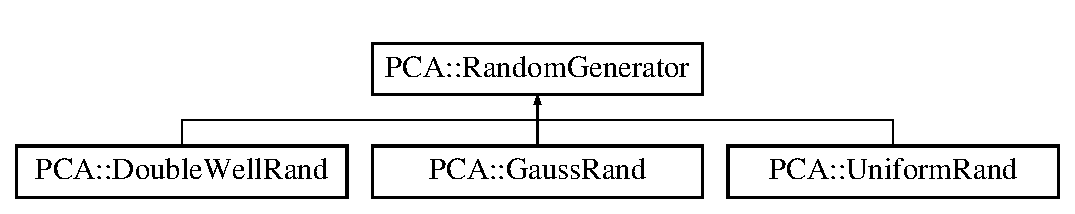
\includegraphics[height=2.000000cm]{class_p_c_a_1_1_random_generator}
\end{center}
\end{figure}
\subsection*{Public Member Functions}
\begin{DoxyCompactItemize}
\item 
virtual double \hyperlink{class_p_c_a_1_1_random_generator_a4361e39397900ae1e7b2cfa91a592509}{operator()} ()=0
\end{DoxyCompactItemize}
\subsection*{Static Public Member Functions}
\begin{DoxyCompactItemize}
\item 
static void \hyperlink{class_p_c_a_1_1_random_generator_aa2ea4616dd82da5cf66b8232697ecba8}{initialization} (uint32\+\_\+t seed\+\_\+in)
\end{DoxyCompactItemize}
\subsection*{Static Public Attributes}
\begin{DoxyCompactItemize}
\item 
static uint32\+\_\+t \hyperlink{class_p_c_a_1_1_random_generator_af96d99ba4eaf71b7d33afd2fbdb7c30d}{seed}
\item 
static std\+::mt19937 \hyperlink{class_p_c_a_1_1_random_generator_abfbe847dad295b691364d0197283afb7}{generator}
\end{DoxyCompactItemize}
\subsection*{Protected Member Functions}
\begin{DoxyCompactItemize}
\item 
\hyperlink{class_p_c_a_1_1_random_generator_a98ccf1f040a1f5dd0151f91537549cc0}{Random\+Generator} ()
\item 
\hyperlink{class_p_c_a_1_1_random_generator_a52e3af6bc9b825d1d4e8d463441ba6f7}{$\sim$\+Random\+Generator} ()
\end{DoxyCompactItemize}


\subsection{Detailed Description}
Parent class of other random classes. 

\subsection{Constructor \& Destructor Documentation}
\hypertarget{class_p_c_a_1_1_random_generator_a98ccf1f040a1f5dd0151f91537549cc0}{}\label{class_p_c_a_1_1_random_generator_a98ccf1f040a1f5dd0151f91537549cc0} 
\index{P\+C\+A\+::\+Random\+Generator@{P\+C\+A\+::\+Random\+Generator}!Random\+Generator@{Random\+Generator}}
\index{Random\+Generator@{Random\+Generator}!P\+C\+A\+::\+Random\+Generator@{P\+C\+A\+::\+Random\+Generator}}
\subsubsection{\texorpdfstring{Random\+Generator()}{RandomGenerator()}}
{\footnotesize\ttfamily P\+C\+A\+::\+Random\+Generator\+::\+Random\+Generator (\begin{DoxyParamCaption}{ }\end{DoxyParamCaption})\hspace{0.3cm}{\ttfamily [protected]}}

\hypertarget{class_p_c_a_1_1_random_generator_a52e3af6bc9b825d1d4e8d463441ba6f7}{}\label{class_p_c_a_1_1_random_generator_a52e3af6bc9b825d1d4e8d463441ba6f7} 
\index{P\+C\+A\+::\+Random\+Generator@{P\+C\+A\+::\+Random\+Generator}!````~Random\+Generator@{$\sim$\+Random\+Generator}}
\index{````~Random\+Generator@{$\sim$\+Random\+Generator}!P\+C\+A\+::\+Random\+Generator@{P\+C\+A\+::\+Random\+Generator}}
\subsubsection{\texorpdfstring{$\sim$\+Random\+Generator()}{~RandomGenerator()}}
{\footnotesize\ttfamily P\+C\+A\+::\+Random\+Generator\+::$\sim$\+Random\+Generator (\begin{DoxyParamCaption}{ }\end{DoxyParamCaption})\hspace{0.3cm}{\ttfamily [protected]}}



\subsection{Member Function Documentation}
\hypertarget{class_p_c_a_1_1_random_generator_aa2ea4616dd82da5cf66b8232697ecba8}{}\label{class_p_c_a_1_1_random_generator_aa2ea4616dd82da5cf66b8232697ecba8} 
\index{P\+C\+A\+::\+Random\+Generator@{P\+C\+A\+::\+Random\+Generator}!initialization@{initialization}}
\index{initialization@{initialization}!P\+C\+A\+::\+Random\+Generator@{P\+C\+A\+::\+Random\+Generator}}
\subsubsection{\texorpdfstring{initialization()}{initialization()}}
{\footnotesize\ttfamily void P\+C\+A\+::\+Random\+Generator\+::initialization (\begin{DoxyParamCaption}\item[{uint32\+\_\+t}]{seed\+\_\+in }\end{DoxyParamCaption})\hspace{0.3cm}{\ttfamily [static]}}

\hypertarget{class_p_c_a_1_1_random_generator_a4361e39397900ae1e7b2cfa91a592509}{}\label{class_p_c_a_1_1_random_generator_a4361e39397900ae1e7b2cfa91a592509} 
\index{P\+C\+A\+::\+Random\+Generator@{P\+C\+A\+::\+Random\+Generator}!operator()@{operator()}}
\index{operator()@{operator()}!P\+C\+A\+::\+Random\+Generator@{P\+C\+A\+::\+Random\+Generator}}
\subsubsection{\texorpdfstring{operator()()}{operator()()}}
{\footnotesize\ttfamily virtual double P\+C\+A\+::\+Random\+Generator\+::operator() (\begin{DoxyParamCaption}{ }\end{DoxyParamCaption})\hspace{0.3cm}{\ttfamily [pure virtual]}}



Implemented in \hyperlink{class_p_c_a_1_1_double_well_rand_a13beb4ae56cd6ccb1d6e4c1e2a03ff9b}{P\+C\+A\+::\+Double\+Well\+Rand}, \hyperlink{class_p_c_a_1_1_gauss_rand_a594130952a4999972f08b429ea6af959}{P\+C\+A\+::\+Gauss\+Rand}, and \hyperlink{class_p_c_a_1_1_uniform_rand_a25b9b060f2201800a5badfa2b70d0eed}{P\+C\+A\+::\+Uniform\+Rand}.



\subsection{Member Data Documentation}
\hypertarget{class_p_c_a_1_1_random_generator_abfbe847dad295b691364d0197283afb7}{}\label{class_p_c_a_1_1_random_generator_abfbe847dad295b691364d0197283afb7} 
\index{P\+C\+A\+::\+Random\+Generator@{P\+C\+A\+::\+Random\+Generator}!generator@{generator}}
\index{generator@{generator}!P\+C\+A\+::\+Random\+Generator@{P\+C\+A\+::\+Random\+Generator}}
\subsubsection{\texorpdfstring{generator}{generator}}
{\footnotesize\ttfamily std\+::mt19937 P\+C\+A\+::\+Random\+Generator\+::generator\hspace{0.3cm}{\ttfamily [static]}}

\hypertarget{class_p_c_a_1_1_random_generator_af96d99ba4eaf71b7d33afd2fbdb7c30d}{}\label{class_p_c_a_1_1_random_generator_af96d99ba4eaf71b7d33afd2fbdb7c30d} 
\index{P\+C\+A\+::\+Random\+Generator@{P\+C\+A\+::\+Random\+Generator}!seed@{seed}}
\index{seed@{seed}!P\+C\+A\+::\+Random\+Generator@{P\+C\+A\+::\+Random\+Generator}}
\subsubsection{\texorpdfstring{seed}{seed}}
{\footnotesize\ttfamily uint32\+\_\+t P\+C\+A\+::\+Random\+Generator\+::seed\hspace{0.3cm}{\ttfamily [static]}}



The documentation for this class was generated from the following files\+:\begin{DoxyCompactItemize}
\item 
/\+Users/annsi118/\+Documents/\+Git\+\_\+projects/\+P\+C\+M\+C/include/\+Random/\hyperlink{_random_generator_8h}{Random\+Generator.\+h}\item 
/\+Users/annsi118/\+Documents/\+Git\+\_\+projects/\+P\+C\+M\+C/source/\+Random/\hyperlink{_random_generator_8cpp}{Random\+Generator.\+cpp}\end{DoxyCompactItemize}

\hypertarget{class_p_c_a_1_1_step_function_calculator}{}\section{P\+CA\+:\+:Step\+Function\+Calculator Class Reference}
\label{class_p_c_a_1_1_step_function_calculator}\index{P\+C\+A\+::\+Step\+Function\+Calculator@{P\+C\+A\+::\+Step\+Function\+Calculator}}


{\ttfamily \#include $<$Step\+Function\+Calculator.\+h$>$}

Inheritance diagram for P\+CA\+:\+:Step\+Function\+Calculator\+:\begin{figure}[H]
\begin{center}
\leavevmode
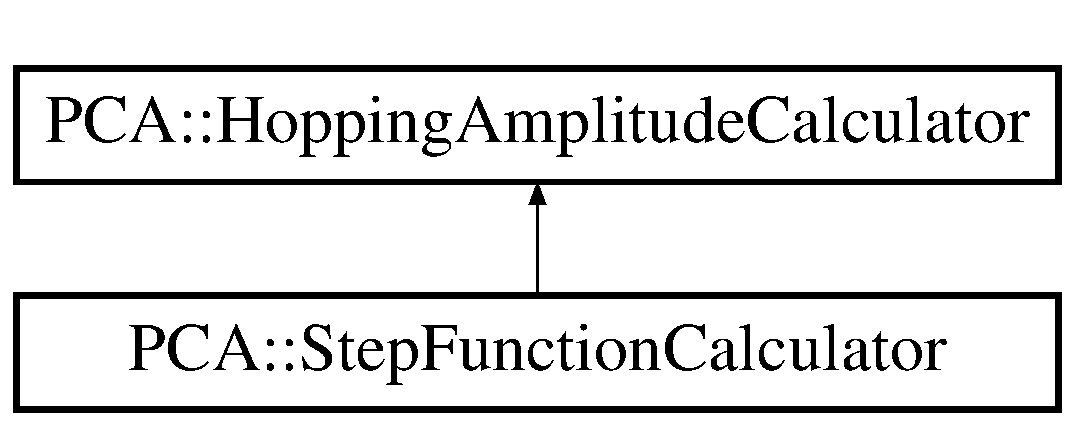
\includegraphics[height=2.000000cm]{class_p_c_a_1_1_step_function_calculator}
\end{center}
\end{figure}
\subsection*{Public Member Functions}
\begin{DoxyCompactItemize}
\item 
\hyperlink{class_p_c_a_1_1_step_function_calculator_a9bf57193b40bb2b8a33fd5a5878b0b2a}{Step\+Function\+Calculator} (double heigth\+\_\+in, double width\+In\+Monomer\+Length, double monomer\+Length)
\item 
\hyperlink{class_p_c_a_1_1_step_function_calculator_a8f3de89d75389034ca485219ce74275b}{$\sim$\+Step\+Function\+Calculator} ()
\item 
std\+::complex$<$ double $>$ \hyperlink{class_p_c_a_1_1_step_function_calculator_a0607e2f78b6b7c0ed40083f921b58fdc}{calculate\+HA} (double distance) const
\end{DoxyCompactItemize}
\subsection*{Private Attributes}
\begin{DoxyCompactItemize}
\item 
double \hyperlink{class_p_c_a_1_1_step_function_calculator_a856f54997b5f0bfbe81040fa55f09146}{height}
\item 
double \hyperlink{class_p_c_a_1_1_step_function_calculator_a777b92937ec96bdc1dc8f887affcb8b3}{width}
\end{DoxyCompactItemize}


\subsection{Constructor \& Destructor Documentation}
\hypertarget{class_p_c_a_1_1_step_function_calculator_a9bf57193b40bb2b8a33fd5a5878b0b2a}{}\label{class_p_c_a_1_1_step_function_calculator_a9bf57193b40bb2b8a33fd5a5878b0b2a} 
\index{P\+C\+A\+::\+Step\+Function\+Calculator@{P\+C\+A\+::\+Step\+Function\+Calculator}!Step\+Function\+Calculator@{Step\+Function\+Calculator}}
\index{Step\+Function\+Calculator@{Step\+Function\+Calculator}!P\+C\+A\+::\+Step\+Function\+Calculator@{P\+C\+A\+::\+Step\+Function\+Calculator}}
\subsubsection{\texorpdfstring{Step\+Function\+Calculator()}{StepFunctionCalculator()}}
{\footnotesize\ttfamily P\+C\+A\+::\+Step\+Function\+Calculator\+::\+Step\+Function\+Calculator (\begin{DoxyParamCaption}\item[{double}]{heigth\+\_\+in,  }\item[{double}]{width\+In\+Monomer\+Length,  }\item[{double}]{monomer\+Length }\end{DoxyParamCaption})}

\hypertarget{class_p_c_a_1_1_step_function_calculator_a8f3de89d75389034ca485219ce74275b}{}\label{class_p_c_a_1_1_step_function_calculator_a8f3de89d75389034ca485219ce74275b} 
\index{P\+C\+A\+::\+Step\+Function\+Calculator@{P\+C\+A\+::\+Step\+Function\+Calculator}!````~Step\+Function\+Calculator@{$\sim$\+Step\+Function\+Calculator}}
\index{````~Step\+Function\+Calculator@{$\sim$\+Step\+Function\+Calculator}!P\+C\+A\+::\+Step\+Function\+Calculator@{P\+C\+A\+::\+Step\+Function\+Calculator}}
\subsubsection{\texorpdfstring{$\sim$\+Step\+Function\+Calculator()}{~StepFunctionCalculator()}}
{\footnotesize\ttfamily P\+C\+A\+::\+Step\+Function\+Calculator\+::$\sim$\+Step\+Function\+Calculator (\begin{DoxyParamCaption}{ }\end{DoxyParamCaption})}



\subsection{Member Function Documentation}
\hypertarget{class_p_c_a_1_1_step_function_calculator_a0607e2f78b6b7c0ed40083f921b58fdc}{}\label{class_p_c_a_1_1_step_function_calculator_a0607e2f78b6b7c0ed40083f921b58fdc} 
\index{P\+C\+A\+::\+Step\+Function\+Calculator@{P\+C\+A\+::\+Step\+Function\+Calculator}!calculate\+HA@{calculate\+HA}}
\index{calculate\+HA@{calculate\+HA}!P\+C\+A\+::\+Step\+Function\+Calculator@{P\+C\+A\+::\+Step\+Function\+Calculator}}
\subsubsection{\texorpdfstring{calculate\+H\+A()}{calculateHA()}}
{\footnotesize\ttfamily std\+::complex$<$ double $>$ P\+C\+A\+::\+Step\+Function\+Calculator\+::calculate\+HA (\begin{DoxyParamCaption}\item[{double}]{distance }\end{DoxyParamCaption}) const\hspace{0.3cm}{\ttfamily [virtual]}}



Implements \hyperlink{class_p_c_a_1_1_hopping_amplitude_calculator_ae925735be8ef006f3f8dfdc1a23cae89}{P\+C\+A\+::\+Hopping\+Amplitude\+Calculator}.



\subsection{Member Data Documentation}
\hypertarget{class_p_c_a_1_1_step_function_calculator_a856f54997b5f0bfbe81040fa55f09146}{}\label{class_p_c_a_1_1_step_function_calculator_a856f54997b5f0bfbe81040fa55f09146} 
\index{P\+C\+A\+::\+Step\+Function\+Calculator@{P\+C\+A\+::\+Step\+Function\+Calculator}!height@{height}}
\index{height@{height}!P\+C\+A\+::\+Step\+Function\+Calculator@{P\+C\+A\+::\+Step\+Function\+Calculator}}
\subsubsection{\texorpdfstring{height}{height}}
{\footnotesize\ttfamily double P\+C\+A\+::\+Step\+Function\+Calculator\+::height\hspace{0.3cm}{\ttfamily [private]}}

\hypertarget{class_p_c_a_1_1_step_function_calculator_a777b92937ec96bdc1dc8f887affcb8b3}{}\label{class_p_c_a_1_1_step_function_calculator_a777b92937ec96bdc1dc8f887affcb8b3} 
\index{P\+C\+A\+::\+Step\+Function\+Calculator@{P\+C\+A\+::\+Step\+Function\+Calculator}!width@{width}}
\index{width@{width}!P\+C\+A\+::\+Step\+Function\+Calculator@{P\+C\+A\+::\+Step\+Function\+Calculator}}
\subsubsection{\texorpdfstring{width}{width}}
{\footnotesize\ttfamily double P\+C\+A\+::\+Step\+Function\+Calculator\+::width\hspace{0.3cm}{\ttfamily [private]}}



The documentation for this class was generated from the following files\+:\begin{DoxyCompactItemize}
\item 
/\+Users/annsi118/\+Documents/\+Git\+\_\+projects/\+P\+C\+M\+C/\+P\+C\+M\+C\+\_\+lib/include/\+Quantum/\hyperlink{_step_function_calculator_8h}{Step\+Function\+Calculator.\+h}\item 
/\+Users/annsi118/\+Documents/\+Git\+\_\+projects/\+P\+C\+M\+C/\+P\+C\+M\+C\+\_\+lib/source/\+Quantum/\hyperlink{_step_function_calculator_8cpp}{Step\+Function\+Calculator.\+cpp}\end{DoxyCompactItemize}

\hypertarget{class_p_c_a_1_1_trancated_exp_calculator}{}\section{P\+CA\+:\+:Trancated\+Exp\+Calculator Class Reference}
\label{class_p_c_a_1_1_trancated_exp_calculator}\index{P\+C\+A\+::\+Trancated\+Exp\+Calculator@{P\+C\+A\+::\+Trancated\+Exp\+Calculator}}


t\+\_\+ij = g $\ast$ exp(-\/m $\ast$ r\+\_\+ij) if r\+\_\+ij $<$ width; t\+\_\+ij = 0 otherwise  




{\ttfamily \#include $<$Trancated\+Exp\+Calculator.\+h$>$}

Inheritance diagram for P\+CA\+:\+:Trancated\+Exp\+Calculator\+:\begin{figure}[H]
\begin{center}
\leavevmode
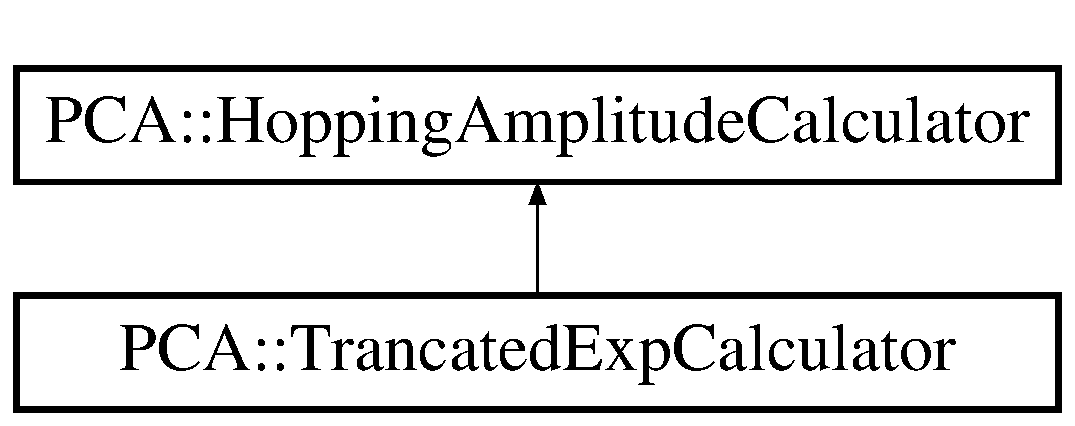
\includegraphics[height=2.000000cm]{class_p_c_a_1_1_trancated_exp_calculator}
\end{center}
\end{figure}
\subsection*{Public Member Functions}
\begin{DoxyCompactItemize}
\item 
\hyperlink{class_p_c_a_1_1_trancated_exp_calculator_a634a2c2d9bc7f54bacf6531f6f8f2c3c}{Trancated\+Exp\+Calculator} (double lambda, double width\+In\+Monomer\+Length, double monomer\+Length)
\item 
\hyperlink{class_p_c_a_1_1_trancated_exp_calculator_a029cab04f65d1a4adebb1dbdf8fd4d3d}{$\sim$\+Trancated\+Exp\+Calculator} ()
\item 
std\+::complex$<$ double $>$ \hyperlink{class_p_c_a_1_1_trancated_exp_calculator_afe48461b23fd2b0d350f32bdac0c3d18}{calculate\+HA} (double distance) const
\end{DoxyCompactItemize}
\subsection*{Private Attributes}
\begin{DoxyCompactItemize}
\item 
double \hyperlink{class_p_c_a_1_1_trancated_exp_calculator_ade1e4dd2be1b5ec6f6e38cc1a251a719}{g}
\item 
double \hyperlink{class_p_c_a_1_1_trancated_exp_calculator_a3d26a4f32c4d4e1ff068cb58446f029d}{m}
\item 
double \hyperlink{class_p_c_a_1_1_trancated_exp_calculator_a18ac7bab1a2ddc18bc214a089d05e4ee}{width}
\end{DoxyCompactItemize}


\subsection{Detailed Description}
t\+\_\+ij = g $\ast$ exp(-\/m $\ast$ r\+\_\+ij) if r\+\_\+ij $<$ width; t\+\_\+ij = 0 otherwise 

g, m will be found from\+: t\+\_\+ij = 1 if r\+\_\+ij = monimer\+Length; t\+\_\+ij = lambda if r\+\_\+ij = 2$\ast$monomer\+Length 

\subsection{Constructor \& Destructor Documentation}
\hypertarget{class_p_c_a_1_1_trancated_exp_calculator_a634a2c2d9bc7f54bacf6531f6f8f2c3c}{}\label{class_p_c_a_1_1_trancated_exp_calculator_a634a2c2d9bc7f54bacf6531f6f8f2c3c} 
\index{P\+C\+A\+::\+Trancated\+Exp\+Calculator@{P\+C\+A\+::\+Trancated\+Exp\+Calculator}!Trancated\+Exp\+Calculator@{Trancated\+Exp\+Calculator}}
\index{Trancated\+Exp\+Calculator@{Trancated\+Exp\+Calculator}!P\+C\+A\+::\+Trancated\+Exp\+Calculator@{P\+C\+A\+::\+Trancated\+Exp\+Calculator}}
\subsubsection{\texorpdfstring{Trancated\+Exp\+Calculator()}{TrancatedExpCalculator()}}
{\footnotesize\ttfamily P\+C\+A\+::\+Trancated\+Exp\+Calculator\+::\+Trancated\+Exp\+Calculator (\begin{DoxyParamCaption}\item[{double}]{lambda,  }\item[{double}]{width\+In\+Monomer\+Length,  }\item[{double}]{monomer\+Length }\end{DoxyParamCaption})}

\hypertarget{class_p_c_a_1_1_trancated_exp_calculator_a029cab04f65d1a4adebb1dbdf8fd4d3d}{}\label{class_p_c_a_1_1_trancated_exp_calculator_a029cab04f65d1a4adebb1dbdf8fd4d3d} 
\index{P\+C\+A\+::\+Trancated\+Exp\+Calculator@{P\+C\+A\+::\+Trancated\+Exp\+Calculator}!````~Trancated\+Exp\+Calculator@{$\sim$\+Trancated\+Exp\+Calculator}}
\index{````~Trancated\+Exp\+Calculator@{$\sim$\+Trancated\+Exp\+Calculator}!P\+C\+A\+::\+Trancated\+Exp\+Calculator@{P\+C\+A\+::\+Trancated\+Exp\+Calculator}}
\subsubsection{\texorpdfstring{$\sim$\+Trancated\+Exp\+Calculator()}{~TrancatedExpCalculator()}}
{\footnotesize\ttfamily P\+C\+A\+::\+Trancated\+Exp\+Calculator\+::$\sim$\+Trancated\+Exp\+Calculator (\begin{DoxyParamCaption}{ }\end{DoxyParamCaption})}



\subsection{Member Function Documentation}
\hypertarget{class_p_c_a_1_1_trancated_exp_calculator_afe48461b23fd2b0d350f32bdac0c3d18}{}\label{class_p_c_a_1_1_trancated_exp_calculator_afe48461b23fd2b0d350f32bdac0c3d18} 
\index{P\+C\+A\+::\+Trancated\+Exp\+Calculator@{P\+C\+A\+::\+Trancated\+Exp\+Calculator}!calculate\+HA@{calculate\+HA}}
\index{calculate\+HA@{calculate\+HA}!P\+C\+A\+::\+Trancated\+Exp\+Calculator@{P\+C\+A\+::\+Trancated\+Exp\+Calculator}}
\subsubsection{\texorpdfstring{calculate\+H\+A()}{calculateHA()}}
{\footnotesize\ttfamily std\+::complex$<$ double $>$ P\+C\+A\+::\+Trancated\+Exp\+Calculator\+::calculate\+HA (\begin{DoxyParamCaption}\item[{double}]{distance }\end{DoxyParamCaption}) const\hspace{0.3cm}{\ttfamily [virtual]}}



Implements \hyperlink{class_p_c_a_1_1_hopping_amplitude_calculator_ae925735be8ef006f3f8dfdc1a23cae89}{P\+C\+A\+::\+Hopping\+Amplitude\+Calculator}.



\subsection{Member Data Documentation}
\hypertarget{class_p_c_a_1_1_trancated_exp_calculator_ade1e4dd2be1b5ec6f6e38cc1a251a719}{}\label{class_p_c_a_1_1_trancated_exp_calculator_ade1e4dd2be1b5ec6f6e38cc1a251a719} 
\index{P\+C\+A\+::\+Trancated\+Exp\+Calculator@{P\+C\+A\+::\+Trancated\+Exp\+Calculator}!g@{g}}
\index{g@{g}!P\+C\+A\+::\+Trancated\+Exp\+Calculator@{P\+C\+A\+::\+Trancated\+Exp\+Calculator}}
\subsubsection{\texorpdfstring{g}{g}}
{\footnotesize\ttfamily double P\+C\+A\+::\+Trancated\+Exp\+Calculator\+::g\hspace{0.3cm}{\ttfamily [private]}}

\hypertarget{class_p_c_a_1_1_trancated_exp_calculator_a3d26a4f32c4d4e1ff068cb58446f029d}{}\label{class_p_c_a_1_1_trancated_exp_calculator_a3d26a4f32c4d4e1ff068cb58446f029d} 
\index{P\+C\+A\+::\+Trancated\+Exp\+Calculator@{P\+C\+A\+::\+Trancated\+Exp\+Calculator}!m@{m}}
\index{m@{m}!P\+C\+A\+::\+Trancated\+Exp\+Calculator@{P\+C\+A\+::\+Trancated\+Exp\+Calculator}}
\subsubsection{\texorpdfstring{m}{m}}
{\footnotesize\ttfamily double P\+C\+A\+::\+Trancated\+Exp\+Calculator\+::m\hspace{0.3cm}{\ttfamily [private]}}

\hypertarget{class_p_c_a_1_1_trancated_exp_calculator_a18ac7bab1a2ddc18bc214a089d05e4ee}{}\label{class_p_c_a_1_1_trancated_exp_calculator_a18ac7bab1a2ddc18bc214a089d05e4ee} 
\index{P\+C\+A\+::\+Trancated\+Exp\+Calculator@{P\+C\+A\+::\+Trancated\+Exp\+Calculator}!width@{width}}
\index{width@{width}!P\+C\+A\+::\+Trancated\+Exp\+Calculator@{P\+C\+A\+::\+Trancated\+Exp\+Calculator}}
\subsubsection{\texorpdfstring{width}{width}}
{\footnotesize\ttfamily double P\+C\+A\+::\+Trancated\+Exp\+Calculator\+::width\hspace{0.3cm}{\ttfamily [private]}}



The documentation for this class was generated from the following files\+:\begin{DoxyCompactItemize}
\item 
/\+Users/annsi118/\+Documents/\+Git\+\_\+projects/\+P\+C\+M\+C/\+P\+C\+M\+C\+\_\+lib/include/\+Quantum/\hyperlink{_trancated_exp_calculator_8h}{Trancated\+Exp\+Calculator.\+h}\item 
/\+Users/annsi118/\+Documents/\+Git\+\_\+projects/\+P\+C\+M\+C/\+P\+C\+M\+C\+\_\+lib/source/\+Quantum/\hyperlink{_trancated_exp_calculator_8cpp}{Trancated\+Exp\+Calculator.\+cpp}\end{DoxyCompactItemize}

\hypertarget{class_p_c_a_1_1_uniform_rand}{}\section{P\+CA\+:\+:Uniform\+Rand Class Reference}
\label{class_p_c_a_1_1_uniform_rand}\index{P\+C\+A\+::\+Uniform\+Rand@{P\+C\+A\+::\+Uniform\+Rand}}


{\ttfamily \#include $<$Uniform\+Rand.\+h$>$}

Inheritance diagram for P\+CA\+:\+:Uniform\+Rand\+:\begin{figure}[H]
\begin{center}
\leavevmode
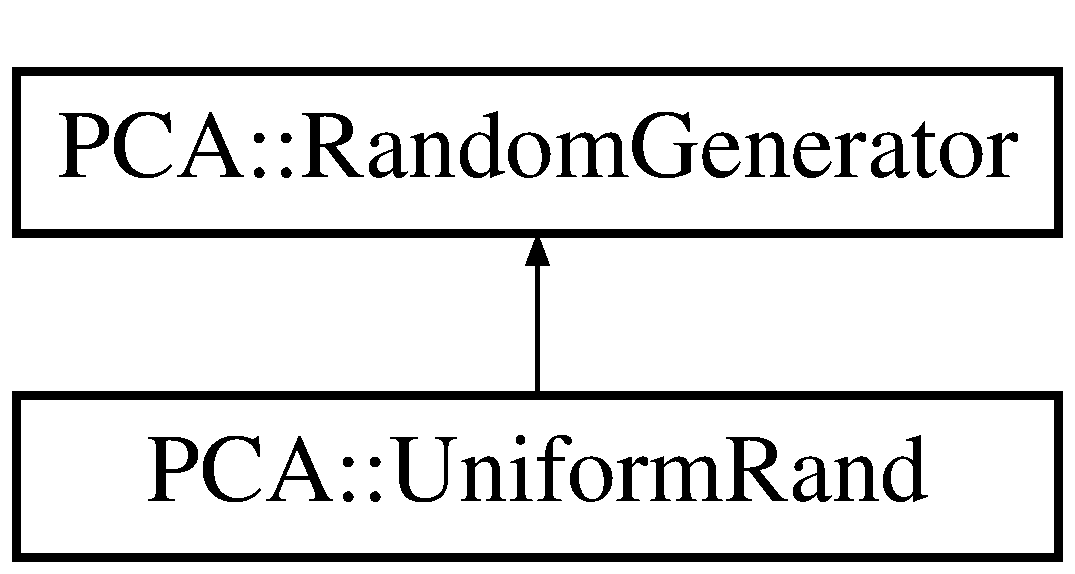
\includegraphics[height=2.000000cm]{class_p_c_a_1_1_uniform_rand}
\end{center}
\end{figure}
\subsection*{Public Member Functions}
\begin{DoxyCompactItemize}
\item 
\hyperlink{class_p_c_a_1_1_uniform_rand_abb80473523980666dd4d5a3f2d5805c1}{Uniform\+Rand} (double min=0.\+0, double max=1.\+0)
\item 
\hyperlink{class_p_c_a_1_1_uniform_rand_ab42f6305d613b61c4b91be3956144a29}{$\sim$\+Uniform\+Rand} ()
\item 
virtual double \hyperlink{class_p_c_a_1_1_uniform_rand_a25b9b060f2201800a5badfa2b70d0eed}{operator()} ()
\begin{DoxyCompactList}\small\item\em overloading operator () \end{DoxyCompactList}\end{DoxyCompactItemize}
\subsection*{Private Attributes}
\begin{DoxyCompactItemize}
\item 
std\+::uniform\+\_\+real\+\_\+distribution$<$ double $>$ \hyperlink{class_p_c_a_1_1_uniform_rand_abf0fad6934be0e79ead12a255a324252}{distribution}
\end{DoxyCompactItemize}
\subsection*{Additional Inherited Members}


\subsection{Constructor \& Destructor Documentation}
\hypertarget{class_p_c_a_1_1_uniform_rand_abb80473523980666dd4d5a3f2d5805c1}{}\label{class_p_c_a_1_1_uniform_rand_abb80473523980666dd4d5a3f2d5805c1} 
\index{P\+C\+A\+::\+Uniform\+Rand@{P\+C\+A\+::\+Uniform\+Rand}!Uniform\+Rand@{Uniform\+Rand}}
\index{Uniform\+Rand@{Uniform\+Rand}!P\+C\+A\+::\+Uniform\+Rand@{P\+C\+A\+::\+Uniform\+Rand}}
\subsubsection{\texorpdfstring{Uniform\+Rand()}{UniformRand()}}
{\footnotesize\ttfamily P\+C\+A\+::\+Uniform\+Rand\+::\+Uniform\+Rand (\begin{DoxyParamCaption}\item[{double}]{min = {\ttfamily 0.0},  }\item[{double}]{max = {\ttfamily 1.0} }\end{DoxyParamCaption})}

\hypertarget{class_p_c_a_1_1_uniform_rand_ab42f6305d613b61c4b91be3956144a29}{}\label{class_p_c_a_1_1_uniform_rand_ab42f6305d613b61c4b91be3956144a29} 
\index{P\+C\+A\+::\+Uniform\+Rand@{P\+C\+A\+::\+Uniform\+Rand}!````~Uniform\+Rand@{$\sim$\+Uniform\+Rand}}
\index{````~Uniform\+Rand@{$\sim$\+Uniform\+Rand}!P\+C\+A\+::\+Uniform\+Rand@{P\+C\+A\+::\+Uniform\+Rand}}
\subsubsection{\texorpdfstring{$\sim$\+Uniform\+Rand()}{~UniformRand()}}
{\footnotesize\ttfamily P\+C\+A\+::\+Uniform\+Rand\+::$\sim$\+Uniform\+Rand (\begin{DoxyParamCaption}{ }\end{DoxyParamCaption})}



\subsection{Member Function Documentation}
\hypertarget{class_p_c_a_1_1_uniform_rand_a25b9b060f2201800a5badfa2b70d0eed}{}\label{class_p_c_a_1_1_uniform_rand_a25b9b060f2201800a5badfa2b70d0eed} 
\index{P\+C\+A\+::\+Uniform\+Rand@{P\+C\+A\+::\+Uniform\+Rand}!operator()@{operator()}}
\index{operator()@{operator()}!P\+C\+A\+::\+Uniform\+Rand@{P\+C\+A\+::\+Uniform\+Rand}}
\subsubsection{\texorpdfstring{operator()()}{operator()()}}
{\footnotesize\ttfamily double P\+C\+A\+::\+Uniform\+Rand\+::operator() (\begin{DoxyParamCaption}{ }\end{DoxyParamCaption})\hspace{0.3cm}{\ttfamily [virtual]}}



overloading operator () 



Implements \hyperlink{class_p_c_a_1_1_random_generator_a4361e39397900ae1e7b2cfa91a592509}{P\+C\+A\+::\+Random\+Generator}.



\subsection{Member Data Documentation}
\hypertarget{class_p_c_a_1_1_uniform_rand_abf0fad6934be0e79ead12a255a324252}{}\label{class_p_c_a_1_1_uniform_rand_abf0fad6934be0e79ead12a255a324252} 
\index{P\+C\+A\+::\+Uniform\+Rand@{P\+C\+A\+::\+Uniform\+Rand}!distribution@{distribution}}
\index{distribution@{distribution}!P\+C\+A\+::\+Uniform\+Rand@{P\+C\+A\+::\+Uniform\+Rand}}
\subsubsection{\texorpdfstring{distribution}{distribution}}
{\footnotesize\ttfamily std\+::uniform\+\_\+real\+\_\+distribution$<$double$>$ P\+C\+A\+::\+Uniform\+Rand\+::distribution\hspace{0.3cm}{\ttfamily [private]}}



The documentation for this class was generated from the following files\+:\begin{DoxyCompactItemize}
\item 
/\+Users/annsi118/\+Documents/\+Git\+\_\+projects/\+P\+C\+M\+C/include/\+Random/\hyperlink{_uniform_rand_8h}{Uniform\+Rand.\+h}\item 
/\+Users/annsi118/\+Documents/\+Git\+\_\+projects/\+P\+C\+M\+C/source/\+Random/\hyperlink{_uniform_rand_8cpp}{Uniform\+Rand.\+cpp}\end{DoxyCompactItemize}

\hypertarget{class_p_c_a_1_1_vector}{}\section{P\+CA\+:\+:Vector Class Reference}
\label{class_p_c_a_1_1_vector}\index{P\+C\+A\+::\+Vector@{P\+C\+A\+::\+Vector}}


{\ttfamily \#include $<$Vector.\+h$>$}

\subsection*{Public Member Functions}
\begin{DoxyCompactItemize}
\item 
\hyperlink{class_p_c_a_1_1_vector_a978077a8e59322b44add93906e551719}{Vector} ()
\item 
\hyperlink{class_p_c_a_1_1_vector_aecc7fa6dbaffa3815fd23e4d8202c9b1}{Vector} (double X, double Y, double Z)
\item 
\hyperlink{class_p_c_a_1_1_vector_a3119a6ed9ccd0d7ac61bdfcbc9b7f1d3}{$\sim$\+Vector} ()
\item 
\hyperlink{class_p_c_a_1_1_vector}{Vector} \& \hyperlink{class_p_c_a_1_1_vector_ac93d124518b0f5e39dd1a0973dddc958}{operator=} (const \hyperlink{class_p_c_a_1_1_vector}{Vector} \&A)
\item 
const \hyperlink{class_p_c_a_1_1_vector}{Vector} \hyperlink{class_p_c_a_1_1_vector_ac94bf46625448a0ece199c2021993e6c}{operator-\/} ()
\item 
bool \hyperlink{class_p_c_a_1_1_vector_ae7a1abe13c8313d717b7bdb66934e92b}{operator==} (const \hyperlink{class_p_c_a_1_1_vector}{Vector} \&A)
\item 
void \hyperlink{class_p_c_a_1_1_vector_a6411d63770d6d711c5c854e21ca1776e}{print} () const
\begin{DoxyCompactList}\small\item\em Print the vector on screen. \end{DoxyCompactList}\item 
void \hyperlink{class_p_c_a_1_1_vector_a661570b8bb883ca11f033ea4dcdebb79}{write\+In\+File} (F\+I\+LE $\ast$fp)
\begin{DoxyCompactList}\small\item\em Write the vector in file. \end{DoxyCompactList}\item 
double \hyperlink{class_p_c_a_1_1_vector_a709eef286197f64e45f35fce0925ddf0}{norm} () const
\end{DoxyCompactItemize}
\subsection*{Static Public Member Functions}
\begin{DoxyCompactItemize}
\item 
static double \hyperlink{class_p_c_a_1_1_vector_abc89550f2ef587f808a7fea91259a22a}{dot\+Product} (const \hyperlink{class_p_c_a_1_1_vector}{Vector} \&A, const \hyperlink{class_p_c_a_1_1_vector}{Vector} \&B)
\item 
static void \hyperlink{class_p_c_a_1_1_vector_a865b60bf89b1dbf3165b8cc503dce2ca}{copy\+Array} (int size, \hyperlink{class_p_c_a_1_1_vector}{Vector} $\ast$vector\+\_\+to, const \hyperlink{class_p_c_a_1_1_vector}{Vector} $\ast$vector\+\_\+from)
\begin{DoxyCompactList}\small\item\em Copy array of size N\+: vector\+\_\+to = vector\+\_\+from. \end{DoxyCompactList}\item 
static void \hyperlink{class_p_c_a_1_1_vector_a385f07b1056ab2a7648b0b9dd03cd8b0}{Kadanoff\+Transformation} (int size, \hyperlink{class_p_c_a_1_1_vector}{Vector} $\ast$vector\+\_\+out, const \hyperlink{class_p_c_a_1_1_vector}{Vector} $\ast$vector\+\_\+in)
\end{DoxyCompactItemize}
\begin{Indent}{\bf Verbose functions\+:}\par
\begin{DoxyCompactItemize}
\item 
static void \hyperlink{class_p_c_a_1_1_vector_a585f8511431df02801aa9cff0e2f1ae4}{set\+Verbose} (bool \hyperlink{class_p_c_a_1_1_vector_a6ef8075198903147f945d0ec81b8defd}{verbose})
\item 
static bool \hyperlink{class_p_c_a_1_1_vector_a06b3f5087a02159bee1f49401db7aad3}{get\+Verbose} ()
\end{DoxyCompactItemize}
\end{Indent}
\subsection*{Public Attributes}
\begin{DoxyCompactItemize}
\item 
double \hyperlink{class_p_c_a_1_1_vector_ac14a3d674fa7956b18a7e2b25aa9b4bb}{x}
\item 
double \hyperlink{class_p_c_a_1_1_vector_a75d5d6af0e3f847456d54412b86c53c0}{y}
\item 
double \hyperlink{class_p_c_a_1_1_vector_a715bde094c7e430c9c39769f6790b835}{z}
\end{DoxyCompactItemize}
\subsection*{Static Public Attributes}
\begin{DoxyCompactItemize}
\item 
static const \hyperlink{class_p_c_a_1_1_vector}{Vector} \hyperlink{class_p_c_a_1_1_vector_a72264553beba4bb7c7a3cea65d4bbd4f}{zero}
\begin{DoxyCompactList}\small\item\em (0.\+0, 0.\+0, 0.\+0) \end{DoxyCompactList}\item 
static const \hyperlink{class_p_c_a_1_1_vector}{Vector} \hyperlink{class_p_c_a_1_1_vector_a2583e534812667f9e5cd69f53569c86b}{eX}
\begin{DoxyCompactList}\small\item\em (1.\+0, 0.\+0, 0.\+0) \end{DoxyCompactList}\item 
static const \hyperlink{class_p_c_a_1_1_vector}{Vector} \hyperlink{class_p_c_a_1_1_vector_ac937f2d1b63ca297cfa3c6d1eac26e1e}{eY}
\begin{DoxyCompactList}\small\item\em (0.\+0, 1.\+0, 0.\+0) \end{DoxyCompactList}\item 
static const \hyperlink{class_p_c_a_1_1_vector}{Vector} \hyperlink{class_p_c_a_1_1_vector_a33a36b16ca1a698b6a0e730222406287}{eZ}
\begin{DoxyCompactList}\small\item\em (0.\+0, 0.\+0, 1.\+0) \end{DoxyCompactList}\end{DoxyCompactItemize}
\subsection*{Static Private Attributes}
\begin{DoxyCompactItemize}
\item 
static bool \hyperlink{class_p_c_a_1_1_vector_a6ef8075198903147f945d0ec81b8defd}{verbose} = true
\begin{DoxyCompactList}\small\item\em If false then this class is not allowed to print anything on screen. \end{DoxyCompactList}\end{DoxyCompactItemize}
\subsection*{Friends}
\begin{DoxyCompactItemize}
\item 
const \hyperlink{class_p_c_a_1_1_vector}{Vector} \hyperlink{class_p_c_a_1_1_vector_a28f83573668a6265c637ee1c77618c84}{operator+} (const \hyperlink{class_p_c_a_1_1_vector}{Vector} \&B, const \hyperlink{class_p_c_a_1_1_vector}{Vector} \&A)
\item 
const \hyperlink{class_p_c_a_1_1_vector}{Vector} \hyperlink{class_p_c_a_1_1_vector_a64185acd75c99c1a3a494a41098fd413}{operator-\/} (const \hyperlink{class_p_c_a_1_1_vector}{Vector} \&B, const \hyperlink{class_p_c_a_1_1_vector}{Vector} \&A)
\item 
const \hyperlink{class_p_c_a_1_1_vector}{Vector} \hyperlink{class_p_c_a_1_1_vector_a89de706cc4a715c026fd01dbee37653c}{operator$\ast$} (const \hyperlink{class_p_c_a_1_1_vector}{Vector} \&B, const \hyperlink{class_p_c_a_1_1_vector}{Vector} \&A)
\begin{DoxyCompactList}\small\item\em cross product \end{DoxyCompactList}\item 
const \hyperlink{class_p_c_a_1_1_vector}{Vector} \hyperlink{class_p_c_a_1_1_vector_af3d0ea67d17d9b5c985d776ed9e54bd5}{operator$\ast$} (double k, const \hyperlink{class_p_c_a_1_1_vector}{Vector} \&A)
\item 
const \hyperlink{class_p_c_a_1_1_vector}{Vector} \hyperlink{class_p_c_a_1_1_vector_a31ae6ac45e0b6192e493d884f271a0d6}{operator$\ast$} (const \hyperlink{class_p_c_a_1_1_vector}{Vector} \&A, double k)
\item 
const \hyperlink{class_p_c_a_1_1_vector}{Vector} \hyperlink{class_p_c_a_1_1_vector_a47572e42d2d4fd6fbe0f891d61809e3b}{operator/} (const \hyperlink{class_p_c_a_1_1_vector}{Vector} \&A, double k)
\end{DoxyCompactItemize}


\subsection{Constructor \& Destructor Documentation}
\hypertarget{class_p_c_a_1_1_vector_a978077a8e59322b44add93906e551719}{}\label{class_p_c_a_1_1_vector_a978077a8e59322b44add93906e551719} 
\index{P\+C\+A\+::\+Vector@{P\+C\+A\+::\+Vector}!Vector@{Vector}}
\index{Vector@{Vector}!P\+C\+A\+::\+Vector@{P\+C\+A\+::\+Vector}}
\subsubsection{\texorpdfstring{Vector()}{Vector()}\hspace{0.1cm}{\footnotesize\ttfamily [1/2]}}
{\footnotesize\ttfamily P\+C\+A\+::\+Vector\+::\+Vector (\begin{DoxyParamCaption}{ }\end{DoxyParamCaption})}

\hypertarget{class_p_c_a_1_1_vector_aecc7fa6dbaffa3815fd23e4d8202c9b1}{}\label{class_p_c_a_1_1_vector_aecc7fa6dbaffa3815fd23e4d8202c9b1} 
\index{P\+C\+A\+::\+Vector@{P\+C\+A\+::\+Vector}!Vector@{Vector}}
\index{Vector@{Vector}!P\+C\+A\+::\+Vector@{P\+C\+A\+::\+Vector}}
\subsubsection{\texorpdfstring{Vector()}{Vector()}\hspace{0.1cm}{\footnotesize\ttfamily [2/2]}}
{\footnotesize\ttfamily P\+C\+A\+::\+Vector\+::\+Vector (\begin{DoxyParamCaption}\item[{double}]{X,  }\item[{double}]{Y,  }\item[{double}]{Z }\end{DoxyParamCaption})}

\hypertarget{class_p_c_a_1_1_vector_a3119a6ed9ccd0d7ac61bdfcbc9b7f1d3}{}\label{class_p_c_a_1_1_vector_a3119a6ed9ccd0d7ac61bdfcbc9b7f1d3} 
\index{P\+C\+A\+::\+Vector@{P\+C\+A\+::\+Vector}!````~Vector@{$\sim$\+Vector}}
\index{````~Vector@{$\sim$\+Vector}!P\+C\+A\+::\+Vector@{P\+C\+A\+::\+Vector}}
\subsubsection{\texorpdfstring{$\sim$\+Vector()}{~Vector()}}
{\footnotesize\ttfamily P\+C\+A\+::\+Vector\+::$\sim$\+Vector (\begin{DoxyParamCaption}{ }\end{DoxyParamCaption})}



\subsection{Member Function Documentation}
\hypertarget{class_p_c_a_1_1_vector_a865b60bf89b1dbf3165b8cc503dce2ca}{}\label{class_p_c_a_1_1_vector_a865b60bf89b1dbf3165b8cc503dce2ca} 
\index{P\+C\+A\+::\+Vector@{P\+C\+A\+::\+Vector}!copy\+Array@{copy\+Array}}
\index{copy\+Array@{copy\+Array}!P\+C\+A\+::\+Vector@{P\+C\+A\+::\+Vector}}
\subsubsection{\texorpdfstring{copy\+Array()}{copyArray()}}
{\footnotesize\ttfamily void P\+C\+A\+::\+Vector\+::copy\+Array (\begin{DoxyParamCaption}\item[{int}]{size,  }\item[{\hyperlink{class_p_c_a_1_1_vector}{Vector} $\ast$}]{vector\+\_\+to,  }\item[{const \hyperlink{class_p_c_a_1_1_vector}{Vector} $\ast$}]{vector\+\_\+from }\end{DoxyParamCaption})\hspace{0.3cm}{\ttfamily [static]}}



Copy array of size N\+: vector\+\_\+to = vector\+\_\+from. 

\hypertarget{class_p_c_a_1_1_vector_abc89550f2ef587f808a7fea91259a22a}{}\label{class_p_c_a_1_1_vector_abc89550f2ef587f808a7fea91259a22a} 
\index{P\+C\+A\+::\+Vector@{P\+C\+A\+::\+Vector}!dot\+Product@{dot\+Product}}
\index{dot\+Product@{dot\+Product}!P\+C\+A\+::\+Vector@{P\+C\+A\+::\+Vector}}
\subsubsection{\texorpdfstring{dot\+Product()}{dotProduct()}}
{\footnotesize\ttfamily double P\+C\+A\+::\+Vector\+::dot\+Product (\begin{DoxyParamCaption}\item[{const \hyperlink{class_p_c_a_1_1_vector}{Vector} \&}]{A,  }\item[{const \hyperlink{class_p_c_a_1_1_vector}{Vector} \&}]{B }\end{DoxyParamCaption})\hspace{0.3cm}{\ttfamily [inline]}, {\ttfamily [static]}}

\hypertarget{class_p_c_a_1_1_vector_a06b3f5087a02159bee1f49401db7aad3}{}\label{class_p_c_a_1_1_vector_a06b3f5087a02159bee1f49401db7aad3} 
\index{P\+C\+A\+::\+Vector@{P\+C\+A\+::\+Vector}!get\+Verbose@{get\+Verbose}}
\index{get\+Verbose@{get\+Verbose}!P\+C\+A\+::\+Vector@{P\+C\+A\+::\+Vector}}
\subsubsection{\texorpdfstring{get\+Verbose()}{getVerbose()}}
{\footnotesize\ttfamily bool P\+C\+A\+::\+Vector\+::get\+Verbose (\begin{DoxyParamCaption}{ }\end{DoxyParamCaption})\hspace{0.3cm}{\ttfamily [static]}}

\hypertarget{class_p_c_a_1_1_vector_a385f07b1056ab2a7648b0b9dd03cd8b0}{}\label{class_p_c_a_1_1_vector_a385f07b1056ab2a7648b0b9dd03cd8b0} 
\index{P\+C\+A\+::\+Vector@{P\+C\+A\+::\+Vector}!Kadanoff\+Transformation@{Kadanoff\+Transformation}}
\index{Kadanoff\+Transformation@{Kadanoff\+Transformation}!P\+C\+A\+::\+Vector@{P\+C\+A\+::\+Vector}}
\subsubsection{\texorpdfstring{Kadanoff\+Transformation()}{KadanoffTransformation()}}
{\footnotesize\ttfamily void P\+C\+A\+::\+Vector\+::\+Kadanoff\+Transformation (\begin{DoxyParamCaption}\item[{int}]{size,  }\item[{\hyperlink{class_p_c_a_1_1_vector}{Vector} $\ast$}]{vector\+\_\+out,  }\item[{const \hyperlink{class_p_c_a_1_1_vector}{Vector} $\ast$}]{vector\+\_\+in }\end{DoxyParamCaption})\hspace{0.3cm}{\ttfamily [static]}}

\hypertarget{class_p_c_a_1_1_vector_a709eef286197f64e45f35fce0925ddf0}{}\label{class_p_c_a_1_1_vector_a709eef286197f64e45f35fce0925ddf0} 
\index{P\+C\+A\+::\+Vector@{P\+C\+A\+::\+Vector}!norm@{norm}}
\index{norm@{norm}!P\+C\+A\+::\+Vector@{P\+C\+A\+::\+Vector}}
\subsubsection{\texorpdfstring{norm()}{norm()}}
{\footnotesize\ttfamily double P\+C\+A\+::\+Vector\+::norm (\begin{DoxyParamCaption}{ }\end{DoxyParamCaption}) const\hspace{0.3cm}{\ttfamily [inline]}}

\hypertarget{class_p_c_a_1_1_vector_ac94bf46625448a0ece199c2021993e6c}{}\label{class_p_c_a_1_1_vector_ac94bf46625448a0ece199c2021993e6c} 
\index{P\+C\+A\+::\+Vector@{P\+C\+A\+::\+Vector}!operator-\/@{operator-\/}}
\index{operator-\/@{operator-\/}!P\+C\+A\+::\+Vector@{P\+C\+A\+::\+Vector}}
\subsubsection{\texorpdfstring{operator-\/()}{operator-()}}
{\footnotesize\ttfamily const \hyperlink{class_p_c_a_1_1_vector}{Vector} P\+C\+A\+::\+Vector\+::operator-\/ (\begin{DoxyParamCaption}{ }\end{DoxyParamCaption})\hspace{0.3cm}{\ttfamily [inline]}}

\hypertarget{class_p_c_a_1_1_vector_ac93d124518b0f5e39dd1a0973dddc958}{}\label{class_p_c_a_1_1_vector_ac93d124518b0f5e39dd1a0973dddc958} 
\index{P\+C\+A\+::\+Vector@{P\+C\+A\+::\+Vector}!operator=@{operator=}}
\index{operator=@{operator=}!P\+C\+A\+::\+Vector@{P\+C\+A\+::\+Vector}}
\subsubsection{\texorpdfstring{operator=()}{operator=()}}
{\footnotesize\ttfamily \hyperlink{class_p_c_a_1_1_vector}{Vector}\& P\+C\+A\+::\+Vector\+::operator= (\begin{DoxyParamCaption}\item[{const \hyperlink{class_p_c_a_1_1_vector}{Vector} \&}]{A }\end{DoxyParamCaption})\hspace{0.3cm}{\ttfamily [inline]}}

\hypertarget{class_p_c_a_1_1_vector_ae7a1abe13c8313d717b7bdb66934e92b}{}\label{class_p_c_a_1_1_vector_ae7a1abe13c8313d717b7bdb66934e92b} 
\index{P\+C\+A\+::\+Vector@{P\+C\+A\+::\+Vector}!operator==@{operator==}}
\index{operator==@{operator==}!P\+C\+A\+::\+Vector@{P\+C\+A\+::\+Vector}}
\subsubsection{\texorpdfstring{operator==()}{operator==()}}
{\footnotesize\ttfamily bool P\+C\+A\+::\+Vector\+::operator== (\begin{DoxyParamCaption}\item[{const \hyperlink{class_p_c_a_1_1_vector}{Vector} \&}]{A }\end{DoxyParamCaption})\hspace{0.3cm}{\ttfamily [inline]}}

\hypertarget{class_p_c_a_1_1_vector_a6411d63770d6d711c5c854e21ca1776e}{}\label{class_p_c_a_1_1_vector_a6411d63770d6d711c5c854e21ca1776e} 
\index{P\+C\+A\+::\+Vector@{P\+C\+A\+::\+Vector}!print@{print}}
\index{print@{print}!P\+C\+A\+::\+Vector@{P\+C\+A\+::\+Vector}}
\subsubsection{\texorpdfstring{print()}{print()}}
{\footnotesize\ttfamily void P\+C\+A\+::\+Vector\+::print (\begin{DoxyParamCaption}{ }\end{DoxyParamCaption}) const}



Print the vector on screen. 

\hypertarget{class_p_c_a_1_1_vector_a585f8511431df02801aa9cff0e2f1ae4}{}\label{class_p_c_a_1_1_vector_a585f8511431df02801aa9cff0e2f1ae4} 
\index{P\+C\+A\+::\+Vector@{P\+C\+A\+::\+Vector}!set\+Verbose@{set\+Verbose}}
\index{set\+Verbose@{set\+Verbose}!P\+C\+A\+::\+Vector@{P\+C\+A\+::\+Vector}}
\subsubsection{\texorpdfstring{set\+Verbose()}{setVerbose()}}
{\footnotesize\ttfamily void P\+C\+A\+::\+Vector\+::set\+Verbose (\begin{DoxyParamCaption}\item[{bool}]{verbose }\end{DoxyParamCaption})\hspace{0.3cm}{\ttfamily [static]}}

\hypertarget{class_p_c_a_1_1_vector_a661570b8bb883ca11f033ea4dcdebb79}{}\label{class_p_c_a_1_1_vector_a661570b8bb883ca11f033ea4dcdebb79} 
\index{P\+C\+A\+::\+Vector@{P\+C\+A\+::\+Vector}!write\+In\+File@{write\+In\+File}}
\index{write\+In\+File@{write\+In\+File}!P\+C\+A\+::\+Vector@{P\+C\+A\+::\+Vector}}
\subsubsection{\texorpdfstring{write\+In\+File()}{writeInFile()}}
{\footnotesize\ttfamily void P\+C\+A\+::\+Vector\+::write\+In\+File (\begin{DoxyParamCaption}\item[{F\+I\+LE $\ast$}]{fp }\end{DoxyParamCaption})\hspace{0.3cm}{\ttfamily [inline]}}



Write the vector in file. 



\subsection{Friends And Related Function Documentation}
\hypertarget{class_p_c_a_1_1_vector_a89de706cc4a715c026fd01dbee37653c}{}\label{class_p_c_a_1_1_vector_a89de706cc4a715c026fd01dbee37653c} 
\index{P\+C\+A\+::\+Vector@{P\+C\+A\+::\+Vector}!operator$\ast$@{operator$\ast$}}
\index{operator$\ast$@{operator$\ast$}!P\+C\+A\+::\+Vector@{P\+C\+A\+::\+Vector}}
\subsubsection{\texorpdfstring{operator$\ast$}{operator*}\hspace{0.1cm}{\footnotesize\ttfamily [1/3]}}
{\footnotesize\ttfamily const \hyperlink{class_p_c_a_1_1_vector}{Vector} operator$\ast$ (\begin{DoxyParamCaption}\item[{const \hyperlink{class_p_c_a_1_1_vector}{Vector} \&}]{B,  }\item[{const \hyperlink{class_p_c_a_1_1_vector}{Vector} \&}]{A }\end{DoxyParamCaption})\hspace{0.3cm}{\ttfamily [friend]}}



cross product 

\hypertarget{class_p_c_a_1_1_vector_af3d0ea67d17d9b5c985d776ed9e54bd5}{}\label{class_p_c_a_1_1_vector_af3d0ea67d17d9b5c985d776ed9e54bd5} 
\index{P\+C\+A\+::\+Vector@{P\+C\+A\+::\+Vector}!operator$\ast$@{operator$\ast$}}
\index{operator$\ast$@{operator$\ast$}!P\+C\+A\+::\+Vector@{P\+C\+A\+::\+Vector}}
\subsubsection{\texorpdfstring{operator$\ast$}{operator*}\hspace{0.1cm}{\footnotesize\ttfamily [2/3]}}
{\footnotesize\ttfamily const \hyperlink{class_p_c_a_1_1_vector}{Vector} operator$\ast$ (\begin{DoxyParamCaption}\item[{double}]{k,  }\item[{const \hyperlink{class_p_c_a_1_1_vector}{Vector} \&}]{A }\end{DoxyParamCaption})\hspace{0.3cm}{\ttfamily [friend]}}

\hypertarget{class_p_c_a_1_1_vector_a31ae6ac45e0b6192e493d884f271a0d6}{}\label{class_p_c_a_1_1_vector_a31ae6ac45e0b6192e493d884f271a0d6} 
\index{P\+C\+A\+::\+Vector@{P\+C\+A\+::\+Vector}!operator$\ast$@{operator$\ast$}}
\index{operator$\ast$@{operator$\ast$}!P\+C\+A\+::\+Vector@{P\+C\+A\+::\+Vector}}
\subsubsection{\texorpdfstring{operator$\ast$}{operator*}\hspace{0.1cm}{\footnotesize\ttfamily [3/3]}}
{\footnotesize\ttfamily const \hyperlink{class_p_c_a_1_1_vector}{Vector} operator$\ast$ (\begin{DoxyParamCaption}\item[{const \hyperlink{class_p_c_a_1_1_vector}{Vector} \&}]{A,  }\item[{double}]{k }\end{DoxyParamCaption})\hspace{0.3cm}{\ttfamily [friend]}}

\hypertarget{class_p_c_a_1_1_vector_a28f83573668a6265c637ee1c77618c84}{}\label{class_p_c_a_1_1_vector_a28f83573668a6265c637ee1c77618c84} 
\index{P\+C\+A\+::\+Vector@{P\+C\+A\+::\+Vector}!operator+@{operator+}}
\index{operator+@{operator+}!P\+C\+A\+::\+Vector@{P\+C\+A\+::\+Vector}}
\subsubsection{\texorpdfstring{operator+}{operator+}}
{\footnotesize\ttfamily const \hyperlink{class_p_c_a_1_1_vector}{Vector} operator+ (\begin{DoxyParamCaption}\item[{const \hyperlink{class_p_c_a_1_1_vector}{Vector} \&}]{B,  }\item[{const \hyperlink{class_p_c_a_1_1_vector}{Vector} \&}]{A }\end{DoxyParamCaption})\hspace{0.3cm}{\ttfamily [friend]}}

\hypertarget{class_p_c_a_1_1_vector_a64185acd75c99c1a3a494a41098fd413}{}\label{class_p_c_a_1_1_vector_a64185acd75c99c1a3a494a41098fd413} 
\index{P\+C\+A\+::\+Vector@{P\+C\+A\+::\+Vector}!operator-\/@{operator-\/}}
\index{operator-\/@{operator-\/}!P\+C\+A\+::\+Vector@{P\+C\+A\+::\+Vector}}
\subsubsection{\texorpdfstring{operator-\/}{operator-}}
{\footnotesize\ttfamily const \hyperlink{class_p_c_a_1_1_vector}{Vector} operator-\/ (\begin{DoxyParamCaption}\item[{const \hyperlink{class_p_c_a_1_1_vector}{Vector} \&}]{B,  }\item[{const \hyperlink{class_p_c_a_1_1_vector}{Vector} \&}]{A }\end{DoxyParamCaption})\hspace{0.3cm}{\ttfamily [friend]}}

\hypertarget{class_p_c_a_1_1_vector_a47572e42d2d4fd6fbe0f891d61809e3b}{}\label{class_p_c_a_1_1_vector_a47572e42d2d4fd6fbe0f891d61809e3b} 
\index{P\+C\+A\+::\+Vector@{P\+C\+A\+::\+Vector}!operator/@{operator/}}
\index{operator/@{operator/}!P\+C\+A\+::\+Vector@{P\+C\+A\+::\+Vector}}
\subsubsection{\texorpdfstring{operator/}{operator/}}
{\footnotesize\ttfamily const \hyperlink{class_p_c_a_1_1_vector}{Vector} operator/ (\begin{DoxyParamCaption}\item[{const \hyperlink{class_p_c_a_1_1_vector}{Vector} \&}]{A,  }\item[{double}]{k }\end{DoxyParamCaption})\hspace{0.3cm}{\ttfamily [friend]}}



\subsection{Member Data Documentation}
\hypertarget{class_p_c_a_1_1_vector_a2583e534812667f9e5cd69f53569c86b}{}\label{class_p_c_a_1_1_vector_a2583e534812667f9e5cd69f53569c86b} 
\index{P\+C\+A\+::\+Vector@{P\+C\+A\+::\+Vector}!eX@{eX}}
\index{eX@{eX}!P\+C\+A\+::\+Vector@{P\+C\+A\+::\+Vector}}
\subsubsection{\texorpdfstring{eX}{eX}}
{\footnotesize\ttfamily const \hyperlink{class_p_c_a_1_1_vector}{Vector} P\+C\+A\+::\+Vector\+::eX\hspace{0.3cm}{\ttfamily [static]}}



(1.\+0, 0.\+0, 0.\+0) 

\hypertarget{class_p_c_a_1_1_vector_ac937f2d1b63ca297cfa3c6d1eac26e1e}{}\label{class_p_c_a_1_1_vector_ac937f2d1b63ca297cfa3c6d1eac26e1e} 
\index{P\+C\+A\+::\+Vector@{P\+C\+A\+::\+Vector}!eY@{eY}}
\index{eY@{eY}!P\+C\+A\+::\+Vector@{P\+C\+A\+::\+Vector}}
\subsubsection{\texorpdfstring{eY}{eY}}
{\footnotesize\ttfamily const \hyperlink{class_p_c_a_1_1_vector}{Vector} P\+C\+A\+::\+Vector\+::eY\hspace{0.3cm}{\ttfamily [static]}}



(0.\+0, 1.\+0, 0.\+0) 

\hypertarget{class_p_c_a_1_1_vector_a33a36b16ca1a698b6a0e730222406287}{}\label{class_p_c_a_1_1_vector_a33a36b16ca1a698b6a0e730222406287} 
\index{P\+C\+A\+::\+Vector@{P\+C\+A\+::\+Vector}!eZ@{eZ}}
\index{eZ@{eZ}!P\+C\+A\+::\+Vector@{P\+C\+A\+::\+Vector}}
\subsubsection{\texorpdfstring{eZ}{eZ}}
{\footnotesize\ttfamily const \hyperlink{class_p_c_a_1_1_vector}{Vector} P\+C\+A\+::\+Vector\+::eZ\hspace{0.3cm}{\ttfamily [static]}}



(0.\+0, 0.\+0, 1.\+0) 

\hypertarget{class_p_c_a_1_1_vector_a6ef8075198903147f945d0ec81b8defd}{}\label{class_p_c_a_1_1_vector_a6ef8075198903147f945d0ec81b8defd} 
\index{P\+C\+A\+::\+Vector@{P\+C\+A\+::\+Vector}!verbose@{verbose}}
\index{verbose@{verbose}!P\+C\+A\+::\+Vector@{P\+C\+A\+::\+Vector}}
\subsubsection{\texorpdfstring{verbose}{verbose}}
{\footnotesize\ttfamily bool P\+C\+A\+::\+Vector\+::verbose = true\hspace{0.3cm}{\ttfamily [static]}, {\ttfamily [private]}}



If false then this class is not allowed to print anything on screen. 

\hypertarget{class_p_c_a_1_1_vector_ac14a3d674fa7956b18a7e2b25aa9b4bb}{}\label{class_p_c_a_1_1_vector_ac14a3d674fa7956b18a7e2b25aa9b4bb} 
\index{P\+C\+A\+::\+Vector@{P\+C\+A\+::\+Vector}!x@{x}}
\index{x@{x}!P\+C\+A\+::\+Vector@{P\+C\+A\+::\+Vector}}
\subsubsection{\texorpdfstring{x}{x}}
{\footnotesize\ttfamily double P\+C\+A\+::\+Vector\+::x}

\hypertarget{class_p_c_a_1_1_vector_a75d5d6af0e3f847456d54412b86c53c0}{}\label{class_p_c_a_1_1_vector_a75d5d6af0e3f847456d54412b86c53c0} 
\index{P\+C\+A\+::\+Vector@{P\+C\+A\+::\+Vector}!y@{y}}
\index{y@{y}!P\+C\+A\+::\+Vector@{P\+C\+A\+::\+Vector}}
\subsubsection{\texorpdfstring{y}{y}}
{\footnotesize\ttfamily double P\+C\+A\+::\+Vector\+::y}

\hypertarget{class_p_c_a_1_1_vector_a715bde094c7e430c9c39769f6790b835}{}\label{class_p_c_a_1_1_vector_a715bde094c7e430c9c39769f6790b835} 
\index{P\+C\+A\+::\+Vector@{P\+C\+A\+::\+Vector}!z@{z}}
\index{z@{z}!P\+C\+A\+::\+Vector@{P\+C\+A\+::\+Vector}}
\subsubsection{\texorpdfstring{z}{z}}
{\footnotesize\ttfamily double P\+C\+A\+::\+Vector\+::z}

\hypertarget{class_p_c_a_1_1_vector_a72264553beba4bb7c7a3cea65d4bbd4f}{}\label{class_p_c_a_1_1_vector_a72264553beba4bb7c7a3cea65d4bbd4f} 
\index{P\+C\+A\+::\+Vector@{P\+C\+A\+::\+Vector}!zero@{zero}}
\index{zero@{zero}!P\+C\+A\+::\+Vector@{P\+C\+A\+::\+Vector}}
\subsubsection{\texorpdfstring{zero}{zero}}
{\footnotesize\ttfamily const \hyperlink{class_p_c_a_1_1_vector}{Vector} P\+C\+A\+::\+Vector\+::zero\hspace{0.3cm}{\ttfamily [static]}}



(0.\+0, 0.\+0, 0.\+0) 



The documentation for this class was generated from the following files\+:\begin{DoxyCompactItemize}
\item 
/\+Users/annsi118/\+Documents/\+Git\+\_\+projects/\+P\+C\+M\+C/include/\hyperlink{_vector_8h}{Vector.\+h}\item 
/\+Users/annsi118/\+Documents/\+Git\+\_\+projects/\+P\+C\+M\+C/source/\hyperlink{_vector_8cpp}{Vector.\+cpp}\end{DoxyCompactItemize}

\hypertarget{class_p_c_a_1_1_yukawa_calculator}{}\section{P\+CA\+:\+:Yukawa\+Calculator Class Reference}
\label{class_p_c_a_1_1_yukawa_calculator}\index{P\+C\+A\+::\+Yukawa\+Calculator@{P\+C\+A\+::\+Yukawa\+Calculator}}


t\+\_\+ij = g $\ast$ exp(-\/m $\ast$ r\+\_\+ij)/ r\+\_\+ij;  




{\ttfamily \#include $<$Yukawa\+Calculator.\+h$>$}

Inheritance diagram for P\+CA\+:\+:Yukawa\+Calculator\+:\begin{figure}[H]
\begin{center}
\leavevmode
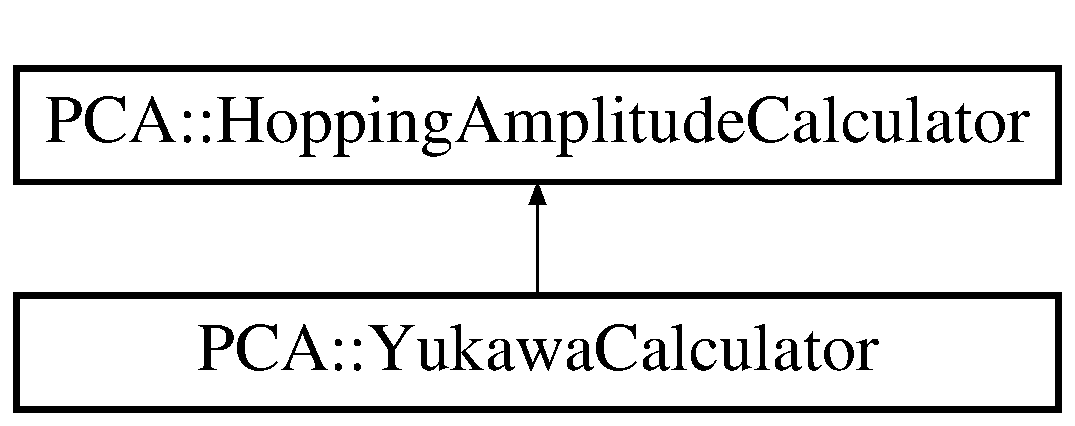
\includegraphics[height=2.000000cm]{class_p_c_a_1_1_yukawa_calculator}
\end{center}
\end{figure}
\subsection*{Public Member Functions}
\begin{DoxyCompactItemize}
\item 
\hyperlink{class_p_c_a_1_1_yukawa_calculator_a8e905580206166f9b63fa24171d48346}{Yukawa\+Calculator} (double lambda, double width\+In\+Monomer\+Length, double monomer\+Length)
\item 
\hyperlink{class_p_c_a_1_1_yukawa_calculator_ab9dcb06991228cb9a48f773ee3375603}{$\sim$\+Yukawa\+Calculator} ()
\item 
std\+::complex$<$ double $>$ \hyperlink{class_p_c_a_1_1_yukawa_calculator_a543f237d55350a7669f8b85789cae68d}{calculate\+HA} (double distance) const
\end{DoxyCompactItemize}
\subsection*{Private Attributes}
\begin{DoxyCompactItemize}
\item 
double \hyperlink{class_p_c_a_1_1_yukawa_calculator_a9fc1cfaf2c30fdd14561238a5b114a0c}{g}
\item 
double \hyperlink{class_p_c_a_1_1_yukawa_calculator_a4b442aa74b079ce8778e19d69c163cf6}{m}
\item 
double \hyperlink{class_p_c_a_1_1_yukawa_calculator_a69e1097584c632e6e43320ef6fc384dc}{width}
\end{DoxyCompactItemize}


\subsection{Detailed Description}
t\+\_\+ij = g $\ast$ exp(-\/m $\ast$ r\+\_\+ij)/ r\+\_\+ij; 

g, m will be found from\+: t\+\_\+ij = 1 if r\+\_\+ij = monimer\+Length; t\+\_\+ij = lambda if r\+\_\+ij = 2$\ast$monomer\+Length 

\subsection{Constructor \& Destructor Documentation}
\hypertarget{class_p_c_a_1_1_yukawa_calculator_a8e905580206166f9b63fa24171d48346}{}\label{class_p_c_a_1_1_yukawa_calculator_a8e905580206166f9b63fa24171d48346} 
\index{P\+C\+A\+::\+Yukawa\+Calculator@{P\+C\+A\+::\+Yukawa\+Calculator}!Yukawa\+Calculator@{Yukawa\+Calculator}}
\index{Yukawa\+Calculator@{Yukawa\+Calculator}!P\+C\+A\+::\+Yukawa\+Calculator@{P\+C\+A\+::\+Yukawa\+Calculator}}
\subsubsection{\texorpdfstring{Yukawa\+Calculator()}{YukawaCalculator()}}
{\footnotesize\ttfamily P\+C\+A\+::\+Yukawa\+Calculator\+::\+Yukawa\+Calculator (\begin{DoxyParamCaption}\item[{double}]{lambda,  }\item[{double}]{width\+In\+Monomer\+Length,  }\item[{double}]{monomer\+Length }\end{DoxyParamCaption})}

\hypertarget{class_p_c_a_1_1_yukawa_calculator_ab9dcb06991228cb9a48f773ee3375603}{}\label{class_p_c_a_1_1_yukawa_calculator_ab9dcb06991228cb9a48f773ee3375603} 
\index{P\+C\+A\+::\+Yukawa\+Calculator@{P\+C\+A\+::\+Yukawa\+Calculator}!````~Yukawa\+Calculator@{$\sim$\+Yukawa\+Calculator}}
\index{````~Yukawa\+Calculator@{$\sim$\+Yukawa\+Calculator}!P\+C\+A\+::\+Yukawa\+Calculator@{P\+C\+A\+::\+Yukawa\+Calculator}}
\subsubsection{\texorpdfstring{$\sim$\+Yukawa\+Calculator()}{~YukawaCalculator()}}
{\footnotesize\ttfamily P\+C\+A\+::\+Yukawa\+Calculator\+::$\sim$\+Yukawa\+Calculator (\begin{DoxyParamCaption}{ }\end{DoxyParamCaption})}



\subsection{Member Function Documentation}
\hypertarget{class_p_c_a_1_1_yukawa_calculator_a543f237d55350a7669f8b85789cae68d}{}\label{class_p_c_a_1_1_yukawa_calculator_a543f237d55350a7669f8b85789cae68d} 
\index{P\+C\+A\+::\+Yukawa\+Calculator@{P\+C\+A\+::\+Yukawa\+Calculator}!calculate\+HA@{calculate\+HA}}
\index{calculate\+HA@{calculate\+HA}!P\+C\+A\+::\+Yukawa\+Calculator@{P\+C\+A\+::\+Yukawa\+Calculator}}
\subsubsection{\texorpdfstring{calculate\+H\+A()}{calculateHA()}}
{\footnotesize\ttfamily std\+::complex$<$ double $>$ P\+C\+A\+::\+Yukawa\+Calculator\+::calculate\+HA (\begin{DoxyParamCaption}\item[{double}]{distance }\end{DoxyParamCaption}) const\hspace{0.3cm}{\ttfamily [virtual]}}



Implements \hyperlink{class_p_c_a_1_1_hopping_amplitude_calculator_ae925735be8ef006f3f8dfdc1a23cae89}{P\+C\+A\+::\+Hopping\+Amplitude\+Calculator}.



\subsection{Member Data Documentation}
\hypertarget{class_p_c_a_1_1_yukawa_calculator_a9fc1cfaf2c30fdd14561238a5b114a0c}{}\label{class_p_c_a_1_1_yukawa_calculator_a9fc1cfaf2c30fdd14561238a5b114a0c} 
\index{P\+C\+A\+::\+Yukawa\+Calculator@{P\+C\+A\+::\+Yukawa\+Calculator}!g@{g}}
\index{g@{g}!P\+C\+A\+::\+Yukawa\+Calculator@{P\+C\+A\+::\+Yukawa\+Calculator}}
\subsubsection{\texorpdfstring{g}{g}}
{\footnotesize\ttfamily double P\+C\+A\+::\+Yukawa\+Calculator\+::g\hspace{0.3cm}{\ttfamily [private]}}

\hypertarget{class_p_c_a_1_1_yukawa_calculator_a4b442aa74b079ce8778e19d69c163cf6}{}\label{class_p_c_a_1_1_yukawa_calculator_a4b442aa74b079ce8778e19d69c163cf6} 
\index{P\+C\+A\+::\+Yukawa\+Calculator@{P\+C\+A\+::\+Yukawa\+Calculator}!m@{m}}
\index{m@{m}!P\+C\+A\+::\+Yukawa\+Calculator@{P\+C\+A\+::\+Yukawa\+Calculator}}
\subsubsection{\texorpdfstring{m}{m}}
{\footnotesize\ttfamily double P\+C\+A\+::\+Yukawa\+Calculator\+::m\hspace{0.3cm}{\ttfamily [private]}}

\hypertarget{class_p_c_a_1_1_yukawa_calculator_a69e1097584c632e6e43320ef6fc384dc}{}\label{class_p_c_a_1_1_yukawa_calculator_a69e1097584c632e6e43320ef6fc384dc} 
\index{P\+C\+A\+::\+Yukawa\+Calculator@{P\+C\+A\+::\+Yukawa\+Calculator}!width@{width}}
\index{width@{width}!P\+C\+A\+::\+Yukawa\+Calculator@{P\+C\+A\+::\+Yukawa\+Calculator}}
\subsubsection{\texorpdfstring{width}{width}}
{\footnotesize\ttfamily double P\+C\+A\+::\+Yukawa\+Calculator\+::width\hspace{0.3cm}{\ttfamily [private]}}



The documentation for this class was generated from the following files\+:\begin{DoxyCompactItemize}
\item 
/\+Users/annsi118/\+Documents/\+Git\+\_\+projects/\+P\+C\+M\+C/\+P\+C\+M\+C\+\_\+lib/include/\+Quantum/\hyperlink{_yukawa_calculator_8h}{Yukawa\+Calculator.\+h}\item 
/\+Users/annsi118/\+Documents/\+Git\+\_\+projects/\+P\+C\+M\+C/\+P\+C\+M\+C\+\_\+lib/source/\+Quantum/\hyperlink{_yukawa_calculator_8cpp}{Yukawa\+Calculator.\+cpp}\end{DoxyCompactItemize}

\chapter{File Documentation}
\hypertarget{_hamiltonian_8h}{}\section{/\+Users/annsi118/\+Documents/\+Git\+\_\+projects/\+P\+C\+M\+C/\+P\+C\+M\+C\+\_\+lib/include/\+Energy/\+Hamiltonian.h File Reference}
\label{_hamiltonian_8h}\index{/\+Users/annsi118/\+Documents/\+Git\+\_\+projects/\+P\+C\+M\+C/\+P\+C\+M\+C\+\_\+lib/include/\+Energy/\+Hamiltonian.\+h@{/\+Users/annsi118/\+Documents/\+Git\+\_\+projects/\+P\+C\+M\+C/\+P\+C\+M\+C\+\_\+lib/include/\+Energy/\+Hamiltonian.\+h}}


Double well potential for kapps angles + gauss for tau angles.  


{\ttfamily \#include \char`\"{}../\+Vector.\+h\char`\"{}}\newline
{\ttfamily \#include \char`\"{}../\+P\+C\+Amacros.\+h\char`\"{}}\newline
{\ttfamily \#include $<$stdlib.\+h$>$}\newline
{\ttfamily \#include $<$stdio.\+h$>$}\newline
\subsection*{Classes}
\begin{DoxyCompactItemize}
\item 
class \hyperlink{class_p_c_a_1_1_hamiltonian}{P\+C\+A\+::\+Hamiltonian}
\begin{DoxyCompactList}\small\item\em \hyperlink{class_p_c_a_1_1_hamiltonian}{Hamiltonian}. \end{DoxyCompactList}\end{DoxyCompactItemize}
\subsection*{Namespaces}
\begin{DoxyCompactItemize}
\item 
 \hyperlink{namespace_p_c_m_c}{P\+C\+MC}
\item 
 \hyperlink{namespace_p_c_a}{P\+CA}
\begin{DoxyCompactList}\small\item\em \hyperlink{_polymer_m_c_8h}{Polymer\+M\+C.\+h}. \end{DoxyCompactList}\end{DoxyCompactItemize}


\subsection{Detailed Description}
Double well potential for kapps angles + gauss for tau angles. 

Anna Sinelnikova  2016 
\hypertarget{_lennard_jones_8h}{}\section{/\+Users/annsi118/\+Documents/\+Git\+\_\+projects/\+P\+C\+M\+C/\+P\+C\+M\+C\+\_\+lib/include/\+Energy/\+Lennard\+Jones.h File Reference}
\label{_lennard_jones_8h}\index{/\+Users/annsi118/\+Documents/\+Git\+\_\+projects/\+P\+C\+M\+C/\+P\+C\+M\+C\+\_\+lib/include/\+Energy/\+Lennard\+Jones.\+h@{/\+Users/annsi118/\+Documents/\+Git\+\_\+projects/\+P\+C\+M\+C/\+P\+C\+M\+C\+\_\+lib/include/\+Energy/\+Lennard\+Jones.\+h}}


Lennard-\/\+Jones potential.  


{\ttfamily \#include \char`\"{}Vector.\+h\char`\"{}}\newline
{\ttfamily \#include \char`\"{}P\+C\+Amacros.\+h\char`\"{}}\newline
{\ttfamily \#include $<$stdlib.\+h$>$}\newline
{\ttfamily \#include $<$stdio.\+h$>$}\newline
\subsection*{Classes}
\begin{DoxyCompactItemize}
\item 
class \hyperlink{class_p_c_a_1_1_lennard_jones}{P\+C\+A\+::\+Lennard\+Jones}
\begin{DoxyCompactList}\small\item\em Lennard-\/\+Jones potential. \end{DoxyCompactList}\end{DoxyCompactItemize}
\subsection*{Namespaces}
\begin{DoxyCompactItemize}
\item 
 \hyperlink{namespace_p_c_m_c}{P\+C\+MC}
\item 
 \hyperlink{namespace_p_c_a}{P\+CA}
\begin{DoxyCompactList}\small\item\em \hyperlink{_polymer_m_c_8h}{Polymer\+M\+C.\+h}. \end{DoxyCompactList}\end{DoxyCompactItemize}


\subsection{Detailed Description}
Lennard-\/\+Jones potential. 

Anna Sinelnikova  2016 
\hypertarget{_file_8h}{}\section{/\+Users/annsi118/\+Documents/\+Git\+\_\+projects/\+P\+C\+M\+C/include/\+File.h File Reference}
\label{_file_8h}\index{/\+Users/annsi118/\+Documents/\+Git\+\_\+projects/\+P\+C\+M\+C/include/\+File.\+h@{/\+Users/annsi118/\+Documents/\+Git\+\_\+projects/\+P\+C\+M\+C/include/\+File.\+h}}


Anna Sinelnikova  2016  


{\ttfamily \#include $<$stdlib.\+h$>$}\newline
{\ttfamily \#include $<$stdio.\+h$>$}\newline
\subsection*{Classes}
\begin{DoxyCompactItemize}
\item 
class \hyperlink{class_p_c_a_1_1_file}{P\+C\+A\+::\+File}
\end{DoxyCompactItemize}
\subsection*{Namespaces}
\begin{DoxyCompactItemize}
\item 
 \hyperlink{namespace_p_c_a}{P\+CA}
\begin{DoxyCompactList}\small\item\em \hyperlink{_polymer_m_c_8h}{Polymer\+M\+C.\+h}. \end{DoxyCompactList}\end{DoxyCompactItemize}


\subsection{Detailed Description}
Anna Sinelnikova  2016 


\hypertarget{_p_c_amacros_8h}{}\section{/\+Users/annsi118/\+Documents/\+Git\+\_\+projects/\+P\+C\+M\+C/\+P\+C\+M\+C\+\_\+lib/include/\+P\+C\+Amacros.h File Reference}
\label{_p_c_amacros_8h}\index{/\+Users/annsi118/\+Documents/\+Git\+\_\+projects/\+P\+C\+M\+C/\+P\+C\+M\+C\+\_\+lib/include/\+P\+C\+Amacros.\+h@{/\+Users/annsi118/\+Documents/\+Git\+\_\+projects/\+P\+C\+M\+C/\+P\+C\+M\+C\+\_\+lib/include/\+P\+C\+Amacros.\+h}}
{\ttfamily \#include $<$stdlib.\+h$>$}\newline
{\ttfamily \#include $<$stdio.\+h$>$}\newline
{\ttfamily \#include $<$math.\+h$>$}\newline
\subsection*{Macros}
\begin{DoxyCompactItemize}
\item 
\#define \hyperlink{_p_c_amacros_8h_a25ee12097a6dd0c586be1dc680326241}{P\+C\+A\+\_\+\+PI}~3.\+141592653589793
\begin{DoxyCompactList}\small\item\em \hyperlink{_p_c_amacros_8h}{P\+C\+Amacros.\+h}. \end{DoxyCompactList}\item 
\#define \hyperlink{_p_c_amacros_8h_a6f53247bb6eed4d90c1fa30a1a55ea86}{\+\_\+\+P\+C\+A\+\_\+\+E\+R\+R\+OR}(function\+Name)
\item 
\#define \hyperlink{_p_c_amacros_8h_ae1443445dffced41c9dfd07bc3f0ad7f}{\+\_\+\+P\+C\+A\+\_\+\+C\+A\+T\+C\+H\+\_\+\+V\+O\+I\+D\+\_\+\+P\+O\+I\+N\+T\+ER}(pointer,  function\+Name)
\item 
\#define \hyperlink{_p_c_amacros_8h_ad13d92940fe21eee8513993f5eb98971}{\+\_\+\+P\+C\+A\+\_\+\+C\+A\+T\+C\+H\+\_\+\+F\+I\+L\+E\+\_\+\+E\+R\+R\+OR}(fp,  action,  file\+Name,  function\+Name)
\item 
\#define \hyperlink{_p_c_amacros_8h_a5540d8f4800a06513afaa6709d6e0578}{P\+C\+A\+\_\+\+N\+U\+M\+E\+R\+I\+C\+A\+L\+\_\+\+E\+R\+R\+OR}~3.\+0$\ast$fabs(atan(1.\+0)-\/\hyperlink{_p_c_amacros_8h_a25ee12097a6dd0c586be1dc680326241}{P\+C\+A\+\_\+\+PI}/4.\+0)
\item 
\#define \hyperlink{_p_c_amacros_8h_ae6b6551a8dd59b4b83fa2ce4b85bd27d}{\+\_\+\+P\+C\+A\+\_\+\+I\+S\+\_\+\+E\+Q\+U\+AL}(a,  b)~fabs(a-\/b)$<$\hyperlink{_p_c_amacros_8h_a5540d8f4800a06513afaa6709d6e0578}{P\+C\+A\+\_\+\+N\+U\+M\+E\+R\+I\+C\+A\+L\+\_\+\+E\+R\+R\+OR}
\end{DoxyCompactItemize}


\subsection{Macro Definition Documentation}
\hypertarget{_p_c_amacros_8h_ad13d92940fe21eee8513993f5eb98971}{}\label{_p_c_amacros_8h_ad13d92940fe21eee8513993f5eb98971} 
\index{P\+C\+Amacros.\+h@{P\+C\+Amacros.\+h}!\+\_\+\+P\+C\+A\+\_\+\+C\+A\+T\+C\+H\+\_\+\+F\+I\+L\+E\+\_\+\+E\+R\+R\+OR@{\+\_\+\+P\+C\+A\+\_\+\+C\+A\+T\+C\+H\+\_\+\+F\+I\+L\+E\+\_\+\+E\+R\+R\+OR}}
\index{\+\_\+\+P\+C\+A\+\_\+\+C\+A\+T\+C\+H\+\_\+\+F\+I\+L\+E\+\_\+\+E\+R\+R\+OR@{\+\_\+\+P\+C\+A\+\_\+\+C\+A\+T\+C\+H\+\_\+\+F\+I\+L\+E\+\_\+\+E\+R\+R\+OR}!P\+C\+Amacros.\+h@{P\+C\+Amacros.\+h}}
\subsubsection{\texorpdfstring{\+\_\+\+P\+C\+A\+\_\+\+C\+A\+T\+C\+H\+\_\+\+F\+I\+L\+E\+\_\+\+E\+R\+R\+OR}{\_PCA\_CATCH\_FILE\_ERROR}}
{\footnotesize\ttfamily \#define \+\_\+\+P\+C\+A\+\_\+\+C\+A\+T\+C\+H\+\_\+\+F\+I\+L\+E\+\_\+\+E\+R\+R\+OR(\begin{DoxyParamCaption}\item[{}]{fp,  }\item[{}]{action,  }\item[{}]{file\+Name,  }\item[{}]{function\+Name }\end{DoxyParamCaption})}

{\bfseries Value\+:}
\begin{DoxyCode}
\textcolor{keywordflow}{if}(fp==NULL)\{\(\backslash\)
    printf(\textcolor{stringliteral}{"Error: cannot \(\backslash\)%s file '%s'\(\backslash\)n\(\backslash\)tin "}, action, fileName);\(\backslash\)
    printf(functionName);\(\backslash\)
    printf(\textcolor{stringliteral}{"\(\backslash\)n"});\(\backslash\)
    exit(1);\(\backslash\)
    \}
\end{DoxyCode}
\hypertarget{_p_c_amacros_8h_ae1443445dffced41c9dfd07bc3f0ad7f}{}\label{_p_c_amacros_8h_ae1443445dffced41c9dfd07bc3f0ad7f} 
\index{P\+C\+Amacros.\+h@{P\+C\+Amacros.\+h}!\+\_\+\+P\+C\+A\+\_\+\+C\+A\+T\+C\+H\+\_\+\+V\+O\+I\+D\+\_\+\+P\+O\+I\+N\+T\+ER@{\+\_\+\+P\+C\+A\+\_\+\+C\+A\+T\+C\+H\+\_\+\+V\+O\+I\+D\+\_\+\+P\+O\+I\+N\+T\+ER}}
\index{\+\_\+\+P\+C\+A\+\_\+\+C\+A\+T\+C\+H\+\_\+\+V\+O\+I\+D\+\_\+\+P\+O\+I\+N\+T\+ER@{\+\_\+\+P\+C\+A\+\_\+\+C\+A\+T\+C\+H\+\_\+\+V\+O\+I\+D\+\_\+\+P\+O\+I\+N\+T\+ER}!P\+C\+Amacros.\+h@{P\+C\+Amacros.\+h}}
\subsubsection{\texorpdfstring{\+\_\+\+P\+C\+A\+\_\+\+C\+A\+T\+C\+H\+\_\+\+V\+O\+I\+D\+\_\+\+P\+O\+I\+N\+T\+ER}{\_PCA\_CATCH\_VOID\_POINTER}}
{\footnotesize\ttfamily \#define \+\_\+\+P\+C\+A\+\_\+\+C\+A\+T\+C\+H\+\_\+\+V\+O\+I\+D\+\_\+\+P\+O\+I\+N\+T\+ER(\begin{DoxyParamCaption}\item[{}]{pointer,  }\item[{}]{function\+Name }\end{DoxyParamCaption})}

{\bfseries Value\+:}
\begin{DoxyCode}
\textcolor{keywordflow}{if}(pointer==NULL)\{\(\backslash\)
    printf(\textcolor{stringliteral}{"Error: void pointer\(\backslash\)n\(\backslash\)tin "});\(\backslash\)
    printf(functionName);\(\backslash\)
    printf(\textcolor{stringliteral}{"\(\backslash\)n"});\(\backslash\)
    exit(1);\(\backslash\)
    \}
\end{DoxyCode}
\hypertarget{_p_c_amacros_8h_a6f53247bb6eed4d90c1fa30a1a55ea86}{}\label{_p_c_amacros_8h_a6f53247bb6eed4d90c1fa30a1a55ea86} 
\index{P\+C\+Amacros.\+h@{P\+C\+Amacros.\+h}!\+\_\+\+P\+C\+A\+\_\+\+E\+R\+R\+OR@{\+\_\+\+P\+C\+A\+\_\+\+E\+R\+R\+OR}}
\index{\+\_\+\+P\+C\+A\+\_\+\+E\+R\+R\+OR@{\+\_\+\+P\+C\+A\+\_\+\+E\+R\+R\+OR}!P\+C\+Amacros.\+h@{P\+C\+Amacros.\+h}}
\subsubsection{\texorpdfstring{\+\_\+\+P\+C\+A\+\_\+\+E\+R\+R\+OR}{\_PCA\_ERROR}}
{\footnotesize\ttfamily \#define \+\_\+\+P\+C\+A\+\_\+\+E\+R\+R\+OR(\begin{DoxyParamCaption}\item[{}]{function\+Name }\end{DoxyParamCaption})}

{\bfseries Value\+:}
\begin{DoxyCode}
\{   printf(\textcolor{stringliteral}{"Error in %s\(\backslash\)n"}, functionName;\(\backslash\)
    exit(1);\(\backslash\)
    \}
\end{DoxyCode}
\hypertarget{_p_c_amacros_8h_ae6b6551a8dd59b4b83fa2ce4b85bd27d}{}\label{_p_c_amacros_8h_ae6b6551a8dd59b4b83fa2ce4b85bd27d} 
\index{P\+C\+Amacros.\+h@{P\+C\+Amacros.\+h}!\+\_\+\+P\+C\+A\+\_\+\+I\+S\+\_\+\+E\+Q\+U\+AL@{\+\_\+\+P\+C\+A\+\_\+\+I\+S\+\_\+\+E\+Q\+U\+AL}}
\index{\+\_\+\+P\+C\+A\+\_\+\+I\+S\+\_\+\+E\+Q\+U\+AL@{\+\_\+\+P\+C\+A\+\_\+\+I\+S\+\_\+\+E\+Q\+U\+AL}!P\+C\+Amacros.\+h@{P\+C\+Amacros.\+h}}
\subsubsection{\texorpdfstring{\+\_\+\+P\+C\+A\+\_\+\+I\+S\+\_\+\+E\+Q\+U\+AL}{\_PCA\_IS\_EQUAL}}
{\footnotesize\ttfamily \#define \+\_\+\+P\+C\+A\+\_\+\+I\+S\+\_\+\+E\+Q\+U\+AL(\begin{DoxyParamCaption}\item[{}]{a,  }\item[{}]{b }\end{DoxyParamCaption})~fabs(a-\/b)$<$\hyperlink{_p_c_amacros_8h_a5540d8f4800a06513afaa6709d6e0578}{P\+C\+A\+\_\+\+N\+U\+M\+E\+R\+I\+C\+A\+L\+\_\+\+E\+R\+R\+OR}}

\hypertarget{_p_c_amacros_8h_a5540d8f4800a06513afaa6709d6e0578}{}\label{_p_c_amacros_8h_a5540d8f4800a06513afaa6709d6e0578} 
\index{P\+C\+Amacros.\+h@{P\+C\+Amacros.\+h}!P\+C\+A\+\_\+\+N\+U\+M\+E\+R\+I\+C\+A\+L\+\_\+\+E\+R\+R\+OR@{P\+C\+A\+\_\+\+N\+U\+M\+E\+R\+I\+C\+A\+L\+\_\+\+E\+R\+R\+OR}}
\index{P\+C\+A\+\_\+\+N\+U\+M\+E\+R\+I\+C\+A\+L\+\_\+\+E\+R\+R\+OR@{P\+C\+A\+\_\+\+N\+U\+M\+E\+R\+I\+C\+A\+L\+\_\+\+E\+R\+R\+OR}!P\+C\+Amacros.\+h@{P\+C\+Amacros.\+h}}
\subsubsection{\texorpdfstring{P\+C\+A\+\_\+\+N\+U\+M\+E\+R\+I\+C\+A\+L\+\_\+\+E\+R\+R\+OR}{PCA\_NUMERICAL\_ERROR}}
{\footnotesize\ttfamily \#define P\+C\+A\+\_\+\+N\+U\+M\+E\+R\+I\+C\+A\+L\+\_\+\+E\+R\+R\+OR~3.\+0$\ast$fabs(atan(1.\+0)-\/\hyperlink{_p_c_amacros_8h_a25ee12097a6dd0c586be1dc680326241}{P\+C\+A\+\_\+\+PI}/4.\+0)}

\hypertarget{_p_c_amacros_8h_a25ee12097a6dd0c586be1dc680326241}{}\label{_p_c_amacros_8h_a25ee12097a6dd0c586be1dc680326241} 
\index{P\+C\+Amacros.\+h@{P\+C\+Amacros.\+h}!P\+C\+A\+\_\+\+PI@{P\+C\+A\+\_\+\+PI}}
\index{P\+C\+A\+\_\+\+PI@{P\+C\+A\+\_\+\+PI}!P\+C\+Amacros.\+h@{P\+C\+Amacros.\+h}}
\subsubsection{\texorpdfstring{P\+C\+A\+\_\+\+PI}{PCA\_PI}}
{\footnotesize\ttfamily \#define P\+C\+A\+\_\+\+PI~3.\+141592653589793}



\hyperlink{_p_c_amacros_8h}{P\+C\+Amacros.\+h}. 

Anna Sinelnikova Uppsala, Sweden 2016 
\hypertarget{_polymer_8h}{}\section{/\+Users/annsi118/\+Documents/\+Git\+\_\+projects/\+P\+C\+M\+C/\+P\+C\+M\+C\+\_\+lib/include/\+Polymer.h File Reference}
\label{_polymer_8h}\index{/\+Users/annsi118/\+Documents/\+Git\+\_\+projects/\+P\+C\+M\+C/\+P\+C\+M\+C\+\_\+lib/include/\+Polymer.\+h@{/\+Users/annsi118/\+Documents/\+Git\+\_\+projects/\+P\+C\+M\+C/\+P\+C\+M\+C\+\_\+lib/include/\+Polymer.\+h}}


Anna Sinelnikova  2016  


{\ttfamily \#include \char`\"{}Vector.\+h\char`\"{}}\newline
{\ttfamily \#include \char`\"{}Utilities.\+h\char`\"{}}\newline
{\ttfamily \#include \char`\"{}P\+C\+Amacros.\+h\char`\"{}}\newline
{\ttfamily \#include $<$stdlib.\+h$>$}\newline
{\ttfamily \#include $<$stdio.\+h$>$}\newline
\subsection*{Classes}
\begin{DoxyCompactItemize}
\item 
class \hyperlink{class_p_c_a_1_1_polymer}{P\+C\+A\+::\+Polymer}
\end{DoxyCompactItemize}
\subsection*{Namespaces}
\begin{DoxyCompactItemize}
\item 
 \hyperlink{namespace_p_c_m_c}{P\+C\+MC}
\item 
 \hyperlink{namespace_p_c_a}{P\+CA}
\begin{DoxyCompactList}\small\item\em \hyperlink{_polymer_m_c_8h}{Polymer\+M\+C.\+h}. \end{DoxyCompactList}\end{DoxyCompactItemize}


\subsection{Detailed Description}
Anna Sinelnikova  2016 


\hypertarget{_polymer_m_c_8h}{}\section{/\+Users/annsi118/\+Documents/\+Git\+\_\+projects/\+P\+C\+M\+C/include/\+Polymer\+MC.h File Reference}
\label{_polymer_m_c_8h}\index{/\+Users/annsi118/\+Documents/\+Git\+\_\+projects/\+P\+C\+M\+C/include/\+Polymer\+M\+C.\+h@{/\+Users/annsi118/\+Documents/\+Git\+\_\+projects/\+P\+C\+M\+C/include/\+Polymer\+M\+C.\+h}}
{\ttfamily \#include \char`\"{}Polymer.\+h\char`\"{}}\newline
{\ttfamily \#include \char`\"{}Vector.\+h\char`\"{}}\newline
{\ttfamily \#include $<$stdlib.\+h$>$}\newline
{\ttfamily \#include $<$stdio.\+h$>$}\newline
\subsection*{Classes}
\begin{DoxyCompactItemize}
\item 
class \hyperlink{class_p_c_a_1_1_polymer_m_c}{P\+C\+A\+::\+Polymer\+MC}
\end{DoxyCompactItemize}
\subsection*{Namespaces}
\begin{DoxyCompactItemize}
\item 
 \hyperlink{namespace_p_c_a}{P\+CA}
\begin{DoxyCompactList}\small\item\em \hyperlink{_polymer_m_c_8h}{Polymer\+M\+C.\+h}. \end{DoxyCompactList}\end{DoxyCompactItemize}

\hypertarget{_polymer_observable_8h}{}\section{/\+Users/annsi118/\+Documents/\+Git\+\_\+projects/\+P\+C\+M\+C/\+P\+C\+M\+C\+\_\+lib/include/\+Polymer\+Observable.h File Reference}
\label{_polymer_observable_8h}\index{/\+Users/annsi118/\+Documents/\+Git\+\_\+projects/\+P\+C\+M\+C/\+P\+C\+M\+C\+\_\+lib/include/\+Polymer\+Observable.\+h@{/\+Users/annsi118/\+Documents/\+Git\+\_\+projects/\+P\+C\+M\+C/\+P\+C\+M\+C\+\_\+lib/include/\+Polymer\+Observable.\+h}}
{\ttfamily \#include \char`\"{}Polymer.\+h\char`\"{}}\newline
{\ttfamily \#include \char`\"{}Vector.\+h\char`\"{}}\newline
{\ttfamily \#include \char`\"{}Utilities.\+h\char`\"{}}\newline
{\ttfamily \#include $<$stdlib.\+h$>$}\newline
{\ttfamily \#include $<$stdio.\+h$>$}\newline
\subsection*{Classes}
\begin{DoxyCompactItemize}
\item 
class \hyperlink{class_p_c_a_1_1_polymer_observable}{P\+C\+A\+::\+Polymer\+Observable}
\end{DoxyCompactItemize}
\subsection*{Namespaces}
\begin{DoxyCompactItemize}
\item 
 \hyperlink{namespace_p_c_a}{P\+CA}
\begin{DoxyCompactList}\small\item\em \hyperlink{_polymer_m_c_8h}{Polymer\+M\+C.\+h}. \end{DoxyCompactList}\end{DoxyCompactItemize}

\hypertarget{_hopping_amplitude_calculator_8h}{}\section{/\+Users/annsi118/\+Documents/\+Git\+\_\+projects/\+P\+C\+M\+C/\+P\+C\+M\+C\+\_\+lib/include/\+Quantum/\+Hopping\+Amplitude\+Calculator.h File Reference}
\label{_hopping_amplitude_calculator_8h}\index{/\+Users/annsi118/\+Documents/\+Git\+\_\+projects/\+P\+C\+M\+C/\+P\+C\+M\+C\+\_\+lib/include/\+Quantum/\+Hopping\+Amplitude\+Calculator.\+h@{/\+Users/annsi118/\+Documents/\+Git\+\_\+projects/\+P\+C\+M\+C/\+P\+C\+M\+C\+\_\+lib/include/\+Quantum/\+Hopping\+Amplitude\+Calculator.\+h}}
{\ttfamily \#include $<$complex$>$}\newline
\subsection*{Classes}
\begin{DoxyCompactItemize}
\item 
class \hyperlink{class_p_c_a_1_1_hopping_amplitude_calculator}{P\+C\+A\+::\+Hopping\+Amplitude\+Calculator}
\end{DoxyCompactItemize}
\subsection*{Namespaces}
\begin{DoxyCompactItemize}
\item 
 \hyperlink{namespace_p_c_a}{P\+CA}
\begin{DoxyCompactList}\small\item\em \hyperlink{_polymer_m_c_8h}{Polymer\+M\+C.\+h}. \end{DoxyCompactList}\end{DoxyCompactItemize}

\hypertarget{_polymer_quantum_8h}{}\section{/\+Users/annsi118/\+Documents/\+Git\+\_\+projects/\+P\+C\+M\+C/\+P\+C\+M\+C\+\_\+lib/include/\+Quantum/\+Polymer\+Quantum.h File Reference}
\label{_polymer_quantum_8h}\index{/\+Users/annsi118/\+Documents/\+Git\+\_\+projects/\+P\+C\+M\+C/\+P\+C\+M\+C\+\_\+lib/include/\+Quantum/\+Polymer\+Quantum.\+h@{/\+Users/annsi118/\+Documents/\+Git\+\_\+projects/\+P\+C\+M\+C/\+P\+C\+M\+C\+\_\+lib/include/\+Quantum/\+Polymer\+Quantum.\+h}}
{\ttfamily \#include \char`\"{}../\+Polymer.\+h\char`\"{}}\newline
{\ttfamily \#include \char`\"{}../\+Vector.\+h\char`\"{}}\newline
{\ttfamily \#include \char`\"{}../\+Utilities.\+h\char`\"{}}\newline
{\ttfamily \#include \char`\"{}Hopping\+Amplitude\+Calculator.\+h\char`\"{}}\newline
{\ttfamily \#include $<$stdlib.\+h$>$}\newline
{\ttfamily \#include $<$stdio.\+h$>$}\newline
{\ttfamily \#include $<$complex$>$}\newline
\subsection*{Classes}
\begin{DoxyCompactItemize}
\item 
class \hyperlink{class_p_c_a_1_1_polymer_quantum}{P\+C\+A\+::\+Polymer\+Quantum}
\end{DoxyCompactItemize}
\subsection*{Namespaces}
\begin{DoxyCompactItemize}
\item 
 \hyperlink{namespace_p_c_a}{P\+CA}
\begin{DoxyCompactList}\small\item\em \hyperlink{_polymer_m_c_8h}{Polymer\+M\+C.\+h}. \end{DoxyCompactList}\end{DoxyCompactItemize}

\hypertarget{_step_function_calculator_8h}{}\section{/\+Users/annsi118/\+Documents/\+Git\+\_\+projects/\+P\+C\+M\+C/\+P\+C\+M\+C\+\_\+lib/include/\+Quantum/\+Step\+Function\+Calculator.h File Reference}
\label{_step_function_calculator_8h}\index{/\+Users/annsi118/\+Documents/\+Git\+\_\+projects/\+P\+C\+M\+C/\+P\+C\+M\+C\+\_\+lib/include/\+Quantum/\+Step\+Function\+Calculator.\+h@{/\+Users/annsi118/\+Documents/\+Git\+\_\+projects/\+P\+C\+M\+C/\+P\+C\+M\+C\+\_\+lib/include/\+Quantum/\+Step\+Function\+Calculator.\+h}}
{\ttfamily \#include \char`\"{}Hopping\+Amplitude\+Calculator.\+h\char`\"{}}\newline
{\ttfamily \#include $<$complex$>$}\newline
\subsection*{Classes}
\begin{DoxyCompactItemize}
\item 
class \hyperlink{class_p_c_a_1_1_step_function_calculator}{P\+C\+A\+::\+Step\+Function\+Calculator}
\end{DoxyCompactItemize}
\subsection*{Namespaces}
\begin{DoxyCompactItemize}
\item 
 \hyperlink{namespace_p_c_a}{P\+CA}
\begin{DoxyCompactList}\small\item\em \hyperlink{_polymer_m_c_8h}{Polymer\+M\+C.\+h}. \end{DoxyCompactList}\end{DoxyCompactItemize}

\hypertarget{_trancated_exp_calculator_8h}{}\section{/\+Users/annsi118/\+Documents/\+Git\+\_\+projects/\+P\+C\+M\+C/include/\+Quantum/\+Trancated\+Exp\+Calculator.h File Reference}
\label{_trancated_exp_calculator_8h}\index{/\+Users/annsi118/\+Documents/\+Git\+\_\+projects/\+P\+C\+M\+C/include/\+Quantum/\+Trancated\+Exp\+Calculator.\+h@{/\+Users/annsi118/\+Documents/\+Git\+\_\+projects/\+P\+C\+M\+C/include/\+Quantum/\+Trancated\+Exp\+Calculator.\+h}}
{\ttfamily \#include \char`\"{}Hopping\+Amplitude\+Calculator.\+h\char`\"{}}\newline
{\ttfamily \#include $<$complex$>$}\newline
\subsection*{Classes}
\begin{DoxyCompactItemize}
\item 
class \hyperlink{class_p_c_a_1_1_trancated_exp_calculator}{P\+C\+A\+::\+Trancated\+Exp\+Calculator}
\begin{DoxyCompactList}\small\item\em t\+\_\+ij = g $\ast$ exp(-\/m $\ast$ r\+\_\+ij) if r\+\_\+ij $<$ width; t\+\_\+ij = 0 otherwise \end{DoxyCompactList}\end{DoxyCompactItemize}
\subsection*{Namespaces}
\begin{DoxyCompactItemize}
\item 
 \hyperlink{namespace_p_c_a}{P\+CA}
\begin{DoxyCompactList}\small\item\em \hyperlink{_polymer_m_c_8h}{Polymer\+M\+C.\+h}. \end{DoxyCompactList}\end{DoxyCompactItemize}

\hypertarget{_yukawa_calculator_8h}{}\section{/\+Users/annsi118/\+Documents/\+Git\+\_\+projects/\+P\+C\+M\+C/\+P\+C\+M\+C\+\_\+lib/include/\+Quantum/\+Yukawa\+Calculator.h File Reference}
\label{_yukawa_calculator_8h}\index{/\+Users/annsi118/\+Documents/\+Git\+\_\+projects/\+P\+C\+M\+C/\+P\+C\+M\+C\+\_\+lib/include/\+Quantum/\+Yukawa\+Calculator.\+h@{/\+Users/annsi118/\+Documents/\+Git\+\_\+projects/\+P\+C\+M\+C/\+P\+C\+M\+C\+\_\+lib/include/\+Quantum/\+Yukawa\+Calculator.\+h}}
{\ttfamily \#include \char`\"{}Hopping\+Amplitude\+Calculator.\+h\char`\"{}}\newline
{\ttfamily \#include $<$complex$>$}\newline
\subsection*{Classes}
\begin{DoxyCompactItemize}
\item 
class \hyperlink{class_p_c_a_1_1_yukawa_calculator}{P\+C\+A\+::\+Yukawa\+Calculator}
\begin{DoxyCompactList}\small\item\em t\+\_\+ij = g $\ast$ exp(-\/m $\ast$ r\+\_\+ij)/ r\+\_\+ij; \end{DoxyCompactList}\end{DoxyCompactItemize}
\subsection*{Namespaces}
\begin{DoxyCompactItemize}
\item 
 \hyperlink{namespace_p_c_a}{P\+CA}
\begin{DoxyCompactList}\small\item\em \hyperlink{_polymer_m_c_8h}{Polymer\+M\+C.\+h}. \end{DoxyCompactList}\end{DoxyCompactItemize}

\hypertarget{_double_well_rand_8h}{}\section{/\+Users/annsi118/\+Documents/\+Git\+\_\+projects/\+P\+C\+M\+C/include/\+Random/\+Double\+Well\+Rand.h File Reference}
\label{_double_well_rand_8h}\index{/\+Users/annsi118/\+Documents/\+Git\+\_\+projects/\+P\+C\+M\+C/include/\+Random/\+Double\+Well\+Rand.\+h@{/\+Users/annsi118/\+Documents/\+Git\+\_\+projects/\+P\+C\+M\+C/include/\+Random/\+Double\+Well\+Rand.\+h}}


Anna Sinelnikova  2016  


{\ttfamily \#include \char`\"{}Uniform\+Rand.\+h\char`\"{}}\newline
\subsection*{Classes}
\begin{DoxyCompactItemize}
\item 
class \hyperlink{class_p_c_a_1_1_double_well_rand}{P\+C\+A\+::\+Double\+Well\+Rand}
\begin{DoxyCompactList}\small\item\em Generate random numbers according distribution\+: \[ P = \exp(-ax^4+bx^2+cx) \] for \[ a>0 \]. \end{DoxyCompactList}\end{DoxyCompactItemize}
\subsection*{Namespaces}
\begin{DoxyCompactItemize}
\item 
 \hyperlink{namespace_p_c_m_c}{P\+C\+MC}
\item 
 \hyperlink{namespace_p_c_a}{P\+CA}
\begin{DoxyCompactList}\small\item\em \hyperlink{_polymer_m_c_8h}{Polymer\+M\+C.\+h}. \end{DoxyCompactList}\end{DoxyCompactItemize}


\subsection{Detailed Description}
Anna Sinelnikova  2016 


\hypertarget{_gauss_rand_8h}{}\section{/\+Users/annsi118/\+Documents/\+Git\+\_\+projects/\+P\+C\+M\+C/\+P\+C\+M\+C\+\_\+lib/include/\+Random/\+Gauss\+Rand.h File Reference}
\label{_gauss_rand_8h}\index{/\+Users/annsi118/\+Documents/\+Git\+\_\+projects/\+P\+C\+M\+C/\+P\+C\+M\+C\+\_\+lib/include/\+Random/\+Gauss\+Rand.\+h@{/\+Users/annsi118/\+Documents/\+Git\+\_\+projects/\+P\+C\+M\+C/\+P\+C\+M\+C\+\_\+lib/include/\+Random/\+Gauss\+Rand.\+h}}


Anna Sinelnikova  2016  


{\ttfamily \#include \char`\"{}Random\+Generator.\+h\char`\"{}}\newline
{\ttfamily \#include $<$random$>$}\newline
\subsection*{Classes}
\begin{DoxyCompactItemize}
\item 
class \hyperlink{class_p_c_a_1_1_gauss_rand}{P\+C\+A\+::\+Gauss\+Rand}
\end{DoxyCompactItemize}
\subsection*{Namespaces}
\begin{DoxyCompactItemize}
\item 
 \hyperlink{namespace_p_c_m_c}{P\+C\+MC}
\item 
 \hyperlink{namespace_p_c_a}{P\+CA}
\begin{DoxyCompactList}\small\item\em \hyperlink{_polymer_m_c_8h}{Polymer\+M\+C.\+h}. \end{DoxyCompactList}\end{DoxyCompactItemize}


\subsection{Detailed Description}
Anna Sinelnikova  2016 


\hypertarget{_random_generator_8h}{}\section{/\+Users/annsi118/\+Documents/\+Git\+\_\+projects/\+P\+C\+M\+C/include/\+Random/\+Random\+Generator.h File Reference}
\label{_random_generator_8h}\index{/\+Users/annsi118/\+Documents/\+Git\+\_\+projects/\+P\+C\+M\+C/include/\+Random/\+Random\+Generator.\+h@{/\+Users/annsi118/\+Documents/\+Git\+\_\+projects/\+P\+C\+M\+C/include/\+Random/\+Random\+Generator.\+h}}


Anna Sinelnikova  2016  


{\ttfamily \#include $<$stdlib.\+h$>$}\newline
{\ttfamily \#include $<$stdio.\+h$>$}\newline
{\ttfamily \#include $<$random$>$}\newline
\subsection*{Classes}
\begin{DoxyCompactItemize}
\item 
class \hyperlink{class_p_c_a_1_1_random_generator}{P\+C\+A\+::\+Random\+Generator}
\begin{DoxyCompactList}\small\item\em Parent class of other random classes. \end{DoxyCompactList}\end{DoxyCompactItemize}
\subsection*{Namespaces}
\begin{DoxyCompactItemize}
\item 
 \hyperlink{namespace_p_c_m_c}{P\+C\+MC}
\item 
 \hyperlink{namespace_p_c_a}{P\+CA}
\begin{DoxyCompactList}\small\item\em \hyperlink{_polymer_m_c_8h}{Polymer\+M\+C.\+h}. \end{DoxyCompactList}\end{DoxyCompactItemize}


\subsection{Detailed Description}
Anna Sinelnikova  2016 


\hypertarget{_uniform_rand_8h}{}\section{/\+Users/annsi118/\+Documents/\+Git\+\_\+projects/\+P\+C\+M\+C/include/\+Random/\+Uniform\+Rand.h File Reference}
\label{_uniform_rand_8h}\index{/\+Users/annsi118/\+Documents/\+Git\+\_\+projects/\+P\+C\+M\+C/include/\+Random/\+Uniform\+Rand.\+h@{/\+Users/annsi118/\+Documents/\+Git\+\_\+projects/\+P\+C\+M\+C/include/\+Random/\+Uniform\+Rand.\+h}}


Anna Sinelnikova  2016  


{\ttfamily \#include \char`\"{}Random\+Generator.\+h\char`\"{}}\newline
{\ttfamily \#include $<$random$>$}\newline
\subsection*{Classes}
\begin{DoxyCompactItemize}
\item 
class \hyperlink{class_p_c_a_1_1_uniform_rand}{P\+C\+A\+::\+Uniform\+Rand}
\end{DoxyCompactItemize}
\subsection*{Namespaces}
\begin{DoxyCompactItemize}
\item 
 \hyperlink{namespace_p_c_m_c}{P\+C\+MC}
\item 
 \hyperlink{namespace_p_c_a}{P\+CA}
\begin{DoxyCompactList}\small\item\em \hyperlink{_polymer_m_c_8h}{Polymer\+M\+C.\+h}. \end{DoxyCompactList}\end{DoxyCompactItemize}


\subsection{Detailed Description}
Anna Sinelnikova  2016 


\hypertarget{_utilities_8h}{}\section{/\+Users/annsi118/\+Documents/\+Git\+\_\+projects/\+P\+C\+M\+C/\+P\+C\+M\+C\+\_\+lib/include/\+Utilities.h File Reference}
\label{_utilities_8h}\index{/\+Users/annsi118/\+Documents/\+Git\+\_\+projects/\+P\+C\+M\+C/\+P\+C\+M\+C\+\_\+lib/include/\+Utilities.\+h@{/\+Users/annsi118/\+Documents/\+Git\+\_\+projects/\+P\+C\+M\+C/\+P\+C\+M\+C\+\_\+lib/include/\+Utilities.\+h}}


Anna Sinelnikova  2016  


{\ttfamily \#include $<$math.\+h$>$}\newline
{\ttfamily \#include \char`\"{}P\+C\+Amacros.\+h\char`\"{}}\newline
\subsection*{Namespaces}
\begin{DoxyCompactItemize}
\item 
 \hyperlink{namespace_p_c_a}{P\+CA}
\begin{DoxyCompactList}\small\item\em \hyperlink{_polymer_m_c_8h}{Polymer\+M\+C.\+h}. \end{DoxyCompactList}\end{DoxyCompactItemize}
\subsection*{Functions}
\begin{DoxyCompactItemize}
\item 
int \hyperlink{namespace_p_c_a_acd05fa0d440ac1781a76499f3cdb3f38}{P\+C\+A\+::rounding} (double number)
\begin{DoxyCompactList}\small\item\em Conventional rounting for doubles. \end{DoxyCompactList}\item 
int \hyperlink{namespace_p_c_a_a13d2c7cbde32faf05da77e81c6396b92}{P\+C\+A\+::common\+Divisor} (int int1, int int2, int upper\+Limit=0)
\begin{DoxyCompactList}\small\item\em Returns common divisor of two numbers which is $<$= upper\+Limit, otherwise 1. \end{DoxyCompactList}\end{DoxyCompactItemize}
\begin{Indent}{\bf Statistics\+:}\par
\begin{DoxyCompactItemize}
\item 
double \hyperlink{namespace_p_c_a_a330e0aee67470237e1e755eb5b151d6c}{P\+C\+A\+::mean\+Value} (int size, const double $\ast$values)
\item 
double \hyperlink{namespace_p_c_a_ae9120f4f9875a87768cc3090196892a8}{P\+C\+A\+::standart\+Deviation} (int size, const double $\ast$values)
\end{DoxyCompactItemize}
\end{Indent}
\begin{Indent}{\bf Work with arrays of doubles}\par
\begin{DoxyCompactItemize}
\item 
void \hyperlink{namespace_p_c_a_ac0ca09771710ce44c06d3f5f4402fd80}{P\+C\+A\+::copy\+Array} (int N, double $\ast$array\+\_\+to, const double $\ast$array\+\_\+from)
\begin{DoxyCompactList}\small\item\em Copy array\+\_\+from of size N to array\+\_\+to of the same size\+: array\+\_\+to = array\+\_\+from. \end{DoxyCompactList}\item 
void \hyperlink{namespace_p_c_a_af4a7844595578d2c8e09635fba6db3b2}{P\+C\+A\+::fill\+Array} (int N, double $\ast$array\+\_\+to, double value)
\end{DoxyCompactItemize}
\end{Indent}
\subsection*{Variables}
\begin{DoxyCompactItemize}
\item 
bool \hyperlink{namespace_p_c_a_a01cf2b18a2d7669f5be721c2142bf67d}{P\+C\+A\+::global\+Verbose} = true
\begin{DoxyCompactList}\small\item\em if false nobody can print on screen. Exseptions\+: error massages, show-\/functions \end{DoxyCompactList}\end{DoxyCompactItemize}


\subsection{Detailed Description}
Anna Sinelnikova  2016 


\hypertarget{_vector_8h}{}\section{/\+Users/annsi118/\+Documents/\+Git\+\_\+projects/\+P\+C\+M\+C/\+P\+C\+M\+C\+\_\+lib/include/\+Vector.h File Reference}
\label{_vector_8h}\index{/\+Users/annsi118/\+Documents/\+Git\+\_\+projects/\+P\+C\+M\+C/\+P\+C\+M\+C\+\_\+lib/include/\+Vector.\+h@{/\+Users/annsi118/\+Documents/\+Git\+\_\+projects/\+P\+C\+M\+C/\+P\+C\+M\+C\+\_\+lib/include/\+Vector.\+h}}


Anna Sinelnikova  2016  


{\ttfamily \#include $<$math.\+h$>$}\newline
{\ttfamily \#include $<$stdio.\+h$>$}\newline
{\ttfamily \#include \char`\"{}Utilities.\+h\char`\"{}}\newline
{\ttfamily \#include \char`\"{}P\+C\+Amacros.\+h\char`\"{}}\newline
\subsection*{Classes}
\begin{DoxyCompactItemize}
\item 
class \hyperlink{class_p_c_a_1_1_vector}{P\+C\+A\+::\+Vector}
\end{DoxyCompactItemize}
\subsection*{Namespaces}
\begin{DoxyCompactItemize}
\item 
 \hyperlink{namespace_p_c_a}{P\+CA}
\begin{DoxyCompactList}\small\item\em \hyperlink{_polymer_m_c_8h}{Polymer\+M\+C.\+h}. \end{DoxyCompactList}\end{DoxyCompactItemize}
\subsection*{Functions}
\begin{DoxyCompactItemize}
\item 
const Vector \hyperlink{namespace_p_c_a_a017b6648f950fd5e297bc92225a425dc}{P\+C\+A\+::operator+} (const Vector \&B, const Vector \&A)
\item 
const Vector \hyperlink{namespace_p_c_a_a430437e74079b33bcf7a99ef38c01134}{P\+C\+A\+::operator-\/} (const Vector \&B, const Vector \&A)
\item 
const Vector \hyperlink{namespace_p_c_a_a49f60e2a8814942d40f8df470c723214}{P\+C\+A\+::operator$\ast$} (const Vector \&B, const Vector \&A)
\item 
const Vector \hyperlink{namespace_p_c_a_a6f1801f8e53ab87a1f3175ec18fa3115}{P\+C\+A\+::operator$\ast$} (double k, const Vector \&A)
\item 
const Vector \hyperlink{namespace_p_c_a_a58012056e60671ce13c8318b3cd1ec8f}{P\+C\+A\+::operator$\ast$} (const Vector \&A, double k)
\item 
const Vector \hyperlink{namespace_p_c_a_a5144cc8f2a3d8ab924e8c4c1c32a2aed}{P\+C\+A\+::operator/} (const Vector \&A, double k)
\end{DoxyCompactItemize}


\subsection{Detailed Description}
Anna Sinelnikova  2016 


\hypertarget{polymer__attract__binary__updates_8h}{}\section{/\+Users/annsi118/\+Documents/\+Git\+\_\+projects/\+P\+C\+M\+C/polymer\+\_\+attract\+\_\+binary\+\_\+updates.h File Reference}
\label{polymer__attract__binary__updates_8h}\index{/\+Users/annsi118/\+Documents/\+Git\+\_\+projects/\+P\+C\+M\+C/polymer\+\_\+attract\+\_\+binary\+\_\+updates.\+h@{/\+Users/annsi118/\+Documents/\+Git\+\_\+projects/\+P\+C\+M\+C/polymer\+\_\+attract\+\_\+binary\+\_\+updates.\+h}}
{\ttfamily \#include \char`\"{}my\+\_\+random.\+h\char`\"{}}\newline
{\ttfamily \#include \char`\"{}vector.\+h\char`\"{}}\newline
{\ttfamily \#include \char`\"{}prob\+\_\+distrib.\+h\char`\"{}}\newline
{\ttfamily \#include $<$cstdlib$>$}\newline
\subsection*{Classes}
\begin{DoxyCompactItemize}
\item 
class \hyperlink{classpolymer}{polymer}
\end{DoxyCompactItemize}
\subsection*{Macros}
\begin{DoxyCompactItemize}
\item 
\#define \hyperlink{polymer__attract__binary__updates_8h_a598a3330b3c21701223ee0ca14316eca}{PI}~3.\+14159265359
\end{DoxyCompactItemize}
\subsection*{Functions}
\begin{DoxyCompactItemize}
\item 
const vector \hyperlink{polymer__attract__binary__updates_8h_ab969bfd08756659f746dce0ced8b183b}{e\+\_\+x} (1, 0, 0)
\item 
const vector \hyperlink{polymer__attract__binary__updates_8h_a7329f71c7f624280a4553802e5d9c9cf}{e\+\_\+y} (0, 1, 0)
\item 
const vector \hyperlink{polymer__attract__binary__updates_8h_aed5a84182b1487c7075aabce4a61504d}{e\+\_\+z} (0, 0, 1)
\item 
vector \hyperlink{polymer__attract__binary__updates_8h_acc5b8702e5bed54e7e15a42748b2602f}{intersection} (vector va, vector vb)
\item 
int \hyperlink{polymer__attract__binary__updates_8h_ae6bf880a796128d830435def1f1baef0}{winding} (double angle)
\end{DoxyCompactItemize}


\subsection{Macro Definition Documentation}
\hypertarget{polymer__attract__binary__updates_8h_a598a3330b3c21701223ee0ca14316eca}{}\label{polymer__attract__binary__updates_8h_a598a3330b3c21701223ee0ca14316eca} 
\index{polymer\+\_\+attract\+\_\+binary\+\_\+updates.\+h@{polymer\+\_\+attract\+\_\+binary\+\_\+updates.\+h}!PI@{PI}}
\index{PI@{PI}!polymer\+\_\+attract\+\_\+binary\+\_\+updates.\+h@{polymer\+\_\+attract\+\_\+binary\+\_\+updates.\+h}}
\subsubsection{\texorpdfstring{PI}{PI}}
{\footnotesize\ttfamily \#define PI~3.\+14159265359}



\subsection{Function Documentation}
\hypertarget{polymer__attract__binary__updates_8h_ab969bfd08756659f746dce0ced8b183b}{}\label{polymer__attract__binary__updates_8h_ab969bfd08756659f746dce0ced8b183b} 
\index{polymer\+\_\+attract\+\_\+binary\+\_\+updates.\+h@{polymer\+\_\+attract\+\_\+binary\+\_\+updates.\+h}!e\+\_\+x@{e\+\_\+x}}
\index{e\+\_\+x@{e\+\_\+x}!polymer\+\_\+attract\+\_\+binary\+\_\+updates.\+h@{polymer\+\_\+attract\+\_\+binary\+\_\+updates.\+h}}
\subsubsection{\texorpdfstring{e\+\_\+x()}{e\_x()}}
{\footnotesize\ttfamily const vector e\+\_\+x (\begin{DoxyParamCaption}\item[{1}]{,  }\item[{0}]{,  }\item[{0}]{ }\end{DoxyParamCaption})}

\hypertarget{polymer__attract__binary__updates_8h_a7329f71c7f624280a4553802e5d9c9cf}{}\label{polymer__attract__binary__updates_8h_a7329f71c7f624280a4553802e5d9c9cf} 
\index{polymer\+\_\+attract\+\_\+binary\+\_\+updates.\+h@{polymer\+\_\+attract\+\_\+binary\+\_\+updates.\+h}!e\+\_\+y@{e\+\_\+y}}
\index{e\+\_\+y@{e\+\_\+y}!polymer\+\_\+attract\+\_\+binary\+\_\+updates.\+h@{polymer\+\_\+attract\+\_\+binary\+\_\+updates.\+h}}
\subsubsection{\texorpdfstring{e\+\_\+y()}{e\_y()}}
{\footnotesize\ttfamily const vector e\+\_\+y (\begin{DoxyParamCaption}\item[{0}]{,  }\item[{1}]{,  }\item[{0}]{ }\end{DoxyParamCaption})}

\hypertarget{polymer__attract__binary__updates_8h_aed5a84182b1487c7075aabce4a61504d}{}\label{polymer__attract__binary__updates_8h_aed5a84182b1487c7075aabce4a61504d} 
\index{polymer\+\_\+attract\+\_\+binary\+\_\+updates.\+h@{polymer\+\_\+attract\+\_\+binary\+\_\+updates.\+h}!e\+\_\+z@{e\+\_\+z}}
\index{e\+\_\+z@{e\+\_\+z}!polymer\+\_\+attract\+\_\+binary\+\_\+updates.\+h@{polymer\+\_\+attract\+\_\+binary\+\_\+updates.\+h}}
\subsubsection{\texorpdfstring{e\+\_\+z()}{e\_z()}}
{\footnotesize\ttfamily const vector e\+\_\+z (\begin{DoxyParamCaption}\item[{0}]{,  }\item[{0}]{,  }\item[{1}]{ }\end{DoxyParamCaption})}

\hypertarget{polymer__attract__binary__updates_8h_acc5b8702e5bed54e7e15a42748b2602f}{}\label{polymer__attract__binary__updates_8h_acc5b8702e5bed54e7e15a42748b2602f} 
\index{polymer\+\_\+attract\+\_\+binary\+\_\+updates.\+h@{polymer\+\_\+attract\+\_\+binary\+\_\+updates.\+h}!intersection@{intersection}}
\index{intersection@{intersection}!polymer\+\_\+attract\+\_\+binary\+\_\+updates.\+h@{polymer\+\_\+attract\+\_\+binary\+\_\+updates.\+h}}
\subsubsection{\texorpdfstring{intersection()}{intersection()}}
{\footnotesize\ttfamily vector intersection (\begin{DoxyParamCaption}\item[{vector}]{va,  }\item[{vector}]{vb }\end{DoxyParamCaption})}

\hypertarget{polymer__attract__binary__updates_8h_ae6bf880a796128d830435def1f1baef0}{}\label{polymer__attract__binary__updates_8h_ae6bf880a796128d830435def1f1baef0} 
\index{polymer\+\_\+attract\+\_\+binary\+\_\+updates.\+h@{polymer\+\_\+attract\+\_\+binary\+\_\+updates.\+h}!winding@{winding}}
\index{winding@{winding}!polymer\+\_\+attract\+\_\+binary\+\_\+updates.\+h@{polymer\+\_\+attract\+\_\+binary\+\_\+updates.\+h}}
\subsubsection{\texorpdfstring{winding()}{winding()}}
{\footnotesize\ttfamily int winding (\begin{DoxyParamCaption}\item[{double}]{angle }\end{DoxyParamCaption})}


\hypertarget{prob__distrib_8h}{}\section{/\+Users/annsi118/\+Documents/\+Git\+\_\+projects/\+P\+C\+M\+C/prob\+\_\+distrib.h File Reference}
\label{prob__distrib_8h}\index{/\+Users/annsi118/\+Documents/\+Git\+\_\+projects/\+P\+C\+M\+C/prob\+\_\+distrib.\+h@{/\+Users/annsi118/\+Documents/\+Git\+\_\+projects/\+P\+C\+M\+C/prob\+\_\+distrib.\+h}}
{\ttfamily \#include $<$stdio.\+h$>$}\newline
{\ttfamily \#include $<$math.\+h$>$}\newline
{\ttfamily \#include $<$stdlib.\+h$>$}\newline
{\ttfamily \#include \char`\"{}gsl/gsl\+\_\+poly.\+h\char`\"{}}\newline
{\ttfamily \#include \char`\"{}gsl/gsl\+\_\+complex.\+h\char`\"{}}\newline
{\ttfamily \#include \char`\"{}gsl/gsl\+\_\+rng.\+h\char`\"{}}\newline
\subsection*{Classes}
\begin{DoxyCompactItemize}
\item 
class \hyperlink{classkappa__distribution}{kappa\+\_\+distribution}
\end{DoxyCompactItemize}

\hypertarget{_r_e_a_d_m_e_8md}{}\section{/\+Users/annsi118/\+Documents/\+Git\+\_\+projects/\+P\+C\+M\+C/\+R\+E\+A\+D\+ME.md File Reference}
\label{_r_e_a_d_m_e_8md}\index{/\+Users/annsi118/\+Documents/\+Git\+\_\+projects/\+P\+C\+M\+C/\+R\+E\+A\+D\+M\+E.\+md@{/\+Users/annsi118/\+Documents/\+Git\+\_\+projects/\+P\+C\+M\+C/\+R\+E\+A\+D\+M\+E.\+md}}

\hypertarget{_hamiltonian_8cpp}{}\section{/\+Users/annsi118/\+Documents/\+Git\+\_\+projects/\+P\+C\+M\+C/\+P\+C\+M\+C\+\_\+lib/source/\+Energy/\+Hamiltonian.cpp File Reference}
\label{_hamiltonian_8cpp}\index{/\+Users/annsi118/\+Documents/\+Git\+\_\+projects/\+P\+C\+M\+C/\+P\+C\+M\+C\+\_\+lib/source/\+Energy/\+Hamiltonian.\+cpp@{/\+Users/annsi118/\+Documents/\+Git\+\_\+projects/\+P\+C\+M\+C/\+P\+C\+M\+C\+\_\+lib/source/\+Energy/\+Hamiltonian.\+cpp}}
{\ttfamily \#include \char`\"{}../../include/\+Energy/\+Hamiltonian.\+h\char`\"{}}\newline
{\ttfamily \#include \char`\"{}../../include/\+Polymer\+M\+C.\+h\char`\"{}}\newline
{\ttfamily \#include \char`\"{}../../include/\+Random/\+Gauss\+Rand.\+h\char`\"{}}\newline
{\ttfamily \#include \char`\"{}../../include/\+Random/\+Double\+Well\+Rand.\+h\char`\"{}}\newline
{\ttfamily \#include \char`\"{}../../include/\+Vector.\+h\char`\"{}}\newline
{\ttfamily \#include \char`\"{}../../include/\+Utilities.\+h\char`\"{}}\newline
{\ttfamily \#include \char`\"{}../../include/\+P\+C\+Amacros.\+h\char`\"{}}\newline
{\ttfamily \#include $<$stdlib.\+h$>$}\newline
{\ttfamily \#include $<$stdio.\+h$>$}\newline
\subsection*{Namespaces}
\begin{DoxyCompactItemize}
\item 
 \hyperlink{namespace_p_c_m_c}{P\+C\+MC}
\item 
 \hyperlink{namespace_p_c_a}{P\+CA}
\begin{DoxyCompactList}\small\item\em \hyperlink{_polymer_m_c_8h}{Polymer\+M\+C.\+h}. \end{DoxyCompactList}\end{DoxyCompactItemize}

\hypertarget{_lennard_jones_8cpp}{}\section{/\+Users/annsi118/\+Documents/\+Git\+\_\+projects/\+P\+C\+M\+C/source/\+Energy/\+Lennard\+Jones.cpp File Reference}
\label{_lennard_jones_8cpp}\index{/\+Users/annsi118/\+Documents/\+Git\+\_\+projects/\+P\+C\+M\+C/source/\+Energy/\+Lennard\+Jones.\+cpp@{/\+Users/annsi118/\+Documents/\+Git\+\_\+projects/\+P\+C\+M\+C/source/\+Energy/\+Lennard\+Jones.\+cpp}}


Lennard-\/\+Jones potential.  


{\ttfamily \#include \char`\"{}Lennard\+Jones.\+h\char`\"{}}\newline
{\ttfamily \#include \char`\"{}Vector.\+h\char`\"{}}\newline
{\ttfamily \#include \char`\"{}Utilities.\+h\char`\"{}}\newline
{\ttfamily \#include \char`\"{}P\+C\+Amacros.\+h\char`\"{}}\newline
{\ttfamily \#include $<$math.\+h$>$}\newline
{\ttfamily \#include $<$stdlib.\+h$>$}\newline
{\ttfamily \#include $<$stdio.\+h$>$}\newline
\subsection*{Namespaces}
\begin{DoxyCompactItemize}
\item 
 \hyperlink{namespace_p_c_m_c}{P\+C\+MC}
\item 
 \hyperlink{namespace_p_c_a}{P\+CA}
\begin{DoxyCompactList}\small\item\em \hyperlink{_polymer_m_c_8h}{Polymer\+M\+C.\+h}. \end{DoxyCompactList}\end{DoxyCompactItemize}


\subsection{Detailed Description}
Lennard-\/\+Jones potential. 

Anna Sinelnikova  2016 
\hypertarget{_file_8cpp}{}\section{/\+Users/annsi118/\+Documents/\+Git\+\_\+projects/\+P\+C\+M\+C/source/\+File.cpp File Reference}
\label{_file_8cpp}\index{/\+Users/annsi118/\+Documents/\+Git\+\_\+projects/\+P\+C\+M\+C/source/\+File.\+cpp@{/\+Users/annsi118/\+Documents/\+Git\+\_\+projects/\+P\+C\+M\+C/source/\+File.\+cpp}}
{\ttfamily \#include \char`\"{}../include/\+File.\+h\char`\"{}}\newline
{\ttfamily \#include \char`\"{}../include/\+Utilities.\+h\char`\"{}}\newline
{\ttfamily \#include \char`\"{}../include/\+P\+C\+Amacros.\+h\char`\"{}}\newline
{\ttfamily \#include $<$math.\+h$>$}\newline
{\ttfamily \#include $<$stdlib.\+h$>$}\newline
{\ttfamily \#include $<$stdio.\+h$>$}\newline
\subsection*{Namespaces}
\begin{DoxyCompactItemize}
\item 
 \hyperlink{namespace_p_c_a}{P\+CA}
\begin{DoxyCompactList}\small\item\em \hyperlink{_polymer_m_c_8h}{Polymer\+M\+C.\+h}. \end{DoxyCompactList}\end{DoxyCompactItemize}

\hypertarget{main_8cpp}{}\section{/\+Users/annsi118/\+Documents/\+Git\+\_\+projects/\+P\+C\+M\+C/source/main.cpp File Reference}
\label{main_8cpp}\index{/\+Users/annsi118/\+Documents/\+Git\+\_\+projects/\+P\+C\+M\+C/source/main.\+cpp@{/\+Users/annsi118/\+Documents/\+Git\+\_\+projects/\+P\+C\+M\+C/source/main.\+cpp}}
{\ttfamily \#include $<$stdio.\+h$>$}\newline
{\ttfamily \#include $<$stdlib.\+h$>$}\newline
{\ttfamily \#include $<$math.\+h$>$}\newline
{\ttfamily \#include \char`\"{}../include/\+Vector.\+h\char`\"{}}\newline
{\ttfamily \#include \char`\"{}../include/\+Utilities.\+h\char`\"{}}\newline
{\ttfamily \#include \char`\"{}../include/\+Polymer.\+h\char`\"{}}\newline
{\ttfamily \#include \char`\"{}../include/\+Polymer\+M\+C.\+h\char`\"{}}\newline
{\ttfamily \#include \char`\"{}../include/\+Random/\+Random\+Generator.\+h\char`\"{}}\newline
{\ttfamily \#include \char`\"{}../include/\+Random/\+Uniform\+Rand.\+h\char`\"{}}\newline
\subsection*{Functions}
\begin{DoxyCompactItemize}
\item 
int \hyperlink{main_8cpp_a86ffaae3870c546d167eee96c59c9e74}{main} (int np, char $\ast$$\ast$p)
\end{DoxyCompactItemize}


\subsection{Function Documentation}
\hypertarget{main_8cpp_a86ffaae3870c546d167eee96c59c9e74}{}\label{main_8cpp_a86ffaae3870c546d167eee96c59c9e74} 
\index{main.\+cpp@{main.\+cpp}!main@{main}}
\index{main@{main}!main.\+cpp@{main.\+cpp}}
\subsubsection{\texorpdfstring{main()}{main()}}
{\footnotesize\ttfamily int main (\begin{DoxyParamCaption}\item[{int}]{np,  }\item[{char $\ast$$\ast$}]{p }\end{DoxyParamCaption})}


\hypertarget{_polymer_8cpp}{}\section{/\+Users/annsi118/\+Documents/\+Git\+\_\+projects/\+P\+C\+M\+C/source/\+Polymer.cpp File Reference}
\label{_polymer_8cpp}\index{/\+Users/annsi118/\+Documents/\+Git\+\_\+projects/\+P\+C\+M\+C/source/\+Polymer.\+cpp@{/\+Users/annsi118/\+Documents/\+Git\+\_\+projects/\+P\+C\+M\+C/source/\+Polymer.\+cpp}}


Anna Sinelnikova  2016  


{\ttfamily \#include \char`\"{}../include/\+Polymer.\+h\char`\"{}}\newline
{\ttfamily \#include \char`\"{}../include/\+P\+C\+Amacros.\+h\char`\"{}}\newline
{\ttfamily \#include \char`\"{}../include/\+Utilities.\+h\char`\"{}}\newline
{\ttfamily \#include \char`\"{}../include/\+File.\+h\char`\"{}}\newline
{\ttfamily \#include $<$stdio.\+h$>$}\newline
{\ttfamily \#include $<$math.\+h$>$}\newline
\subsection*{Namespaces}
\begin{DoxyCompactItemize}
\item 
 \hyperlink{namespace_p_c_m_c}{P\+C\+MC}
\item 
 \hyperlink{namespace_p_c_a}{P\+CA}
\begin{DoxyCompactList}\small\item\em \hyperlink{_polymer_m_c_8h}{Polymer\+M\+C.\+h}. \end{DoxyCompactList}\end{DoxyCompactItemize}


\subsection{Detailed Description}
Anna Sinelnikova  2016 


\hypertarget{_polymer_m_c_8cpp}{}\section{/\+Users/annsi118/\+Documents/\+Git\+\_\+projects/\+P\+C\+M\+C/source/\+Polymer\+MC.cpp File Reference}
\label{_polymer_m_c_8cpp}\index{/\+Users/annsi118/\+Documents/\+Git\+\_\+projects/\+P\+C\+M\+C/source/\+Polymer\+M\+C.\+cpp@{/\+Users/annsi118/\+Documents/\+Git\+\_\+projects/\+P\+C\+M\+C/source/\+Polymer\+M\+C.\+cpp}}
{\ttfamily \#include \char`\"{}../include/\+Polymer\+M\+C.\+h\char`\"{}}\newline
{\ttfamily \#include \char`\"{}../include/\+Polymer.\+h\char`\"{}}\newline
{\ttfamily \#include \char`\"{}../include/\+Vector.\+h\char`\"{}}\newline
{\ttfamily \#include \char`\"{}../include/\+Utilities.\+h\char`\"{}}\newline
{\ttfamily \#include $<$stdio.\+h$>$}\newline
{\ttfamily \#include $<$math.\+h$>$}\newline
\subsection*{Namespaces}
\begin{DoxyCompactItemize}
\item 
 \hyperlink{namespace_p_c_a}{P\+CA}
\begin{DoxyCompactList}\small\item\em \hyperlink{_polymer_m_c_8h}{Polymer\+M\+C.\+h}. \end{DoxyCompactList}\end{DoxyCompactItemize}
\subsection*{Macros}
\begin{DoxyCompactItemize}
\item 
\#define \hyperlink{_polymer_m_c_8cpp_ac427d2eec9809e2d3b13fbedd1a4b2a3}{\+\_\+\+C\+A\+T\+C\+H\+\_\+\+E\+R\+R\+OR}(pointer,  error\+\_\+message)~if(pointer==N\+U\+LL)\{printf(error\+\_\+message);exit(1);\}
\begin{DoxyCompactList}\small\item\em \hyperlink{_polymer_m_c_8cpp}{Polymer\+M\+C.\+cpp}. \end{DoxyCompactList}\end{DoxyCompactItemize}


\subsection{Macro Definition Documentation}
\hypertarget{_polymer_m_c_8cpp_ac427d2eec9809e2d3b13fbedd1a4b2a3}{}\label{_polymer_m_c_8cpp_ac427d2eec9809e2d3b13fbedd1a4b2a3} 
\index{Polymer\+M\+C.\+cpp@{Polymer\+M\+C.\+cpp}!\+\_\+\+C\+A\+T\+C\+H\+\_\+\+E\+R\+R\+OR@{\+\_\+\+C\+A\+T\+C\+H\+\_\+\+E\+R\+R\+OR}}
\index{\+\_\+\+C\+A\+T\+C\+H\+\_\+\+E\+R\+R\+OR@{\+\_\+\+C\+A\+T\+C\+H\+\_\+\+E\+R\+R\+OR}!Polymer\+M\+C.\+cpp@{Polymer\+M\+C.\+cpp}}
\subsubsection{\texorpdfstring{\+\_\+\+C\+A\+T\+C\+H\+\_\+\+E\+R\+R\+OR}{\_CATCH\_ERROR}}
{\footnotesize\ttfamily \#define \+\_\+\+C\+A\+T\+C\+H\+\_\+\+E\+R\+R\+OR(\begin{DoxyParamCaption}\item[{}]{pointer,  }\item[{}]{error\+\_\+message }\end{DoxyParamCaption})~if(pointer==N\+U\+LL)\{printf(error\+\_\+message);exit(1);\}}



\hyperlink{_polymer_m_c_8cpp}{Polymer\+M\+C.\+cpp}. 

Anna Sinelnikova Uppsala, Sweden 2016 
\hypertarget{_polymer_observable_8cpp}{}\section{/\+Users/annsi118/\+Documents/\+Git\+\_\+projects/\+P\+C\+M\+C/source/\+Polymer\+Observable.cpp File Reference}
\label{_polymer_observable_8cpp}\index{/\+Users/annsi118/\+Documents/\+Git\+\_\+projects/\+P\+C\+M\+C/source/\+Polymer\+Observable.\+cpp@{/\+Users/annsi118/\+Documents/\+Git\+\_\+projects/\+P\+C\+M\+C/source/\+Polymer\+Observable.\+cpp}}
{\ttfamily \#include \char`\"{}../include/\+Polymer\+Observable.\+h\char`\"{}}\newline
{\ttfamily \#include \char`\"{}../include/\+Polymer.\+h\char`\"{}}\newline
{\ttfamily \#include \char`\"{}../include/\+Utilities.\+h\char`\"{}}\newline
{\ttfamily \#include $<$stdio.\+h$>$}\newline
{\ttfamily \#include $<$math.\+h$>$}\newline
\subsection*{Namespaces}
\begin{DoxyCompactItemize}
\item 
 \hyperlink{namespace_p_c_a}{P\+CA}
\begin{DoxyCompactList}\small\item\em \hyperlink{_polymer_m_c_8h}{Polymer\+M\+C.\+h}. \end{DoxyCompactList}\end{DoxyCompactItemize}
\subsection*{Macros}
\begin{DoxyCompactItemize}
\item 
\#define \hyperlink{_polymer_observable_8cpp_ac427d2eec9809e2d3b13fbedd1a4b2a3}{\+\_\+\+C\+A\+T\+C\+H\+\_\+\+E\+R\+R\+OR}(pointer,  error\+\_\+message)~if(pointer==N\+U\+LL)\{printf(error\+\_\+message);exit(1);\}
\end{DoxyCompactItemize}


\subsection{Macro Definition Documentation}
\hypertarget{_polymer_observable_8cpp_ac427d2eec9809e2d3b13fbedd1a4b2a3}{}\label{_polymer_observable_8cpp_ac427d2eec9809e2d3b13fbedd1a4b2a3} 
\index{Polymer\+Observable.\+cpp@{Polymer\+Observable.\+cpp}!\+\_\+\+C\+A\+T\+C\+H\+\_\+\+E\+R\+R\+OR@{\+\_\+\+C\+A\+T\+C\+H\+\_\+\+E\+R\+R\+OR}}
\index{\+\_\+\+C\+A\+T\+C\+H\+\_\+\+E\+R\+R\+OR@{\+\_\+\+C\+A\+T\+C\+H\+\_\+\+E\+R\+R\+OR}!Polymer\+Observable.\+cpp@{Polymer\+Observable.\+cpp}}
\subsubsection{\texorpdfstring{\+\_\+\+C\+A\+T\+C\+H\+\_\+\+E\+R\+R\+OR}{\_CATCH\_ERROR}}
{\footnotesize\ttfamily \#define \+\_\+\+C\+A\+T\+C\+H\+\_\+\+E\+R\+R\+OR(\begin{DoxyParamCaption}\item[{}]{pointer,  }\item[{}]{error\+\_\+message }\end{DoxyParamCaption})~if(pointer==N\+U\+LL)\{printf(error\+\_\+message);exit(1);\}}


\hypertarget{_polymer_quantum_8cpp}{}\section{/\+Users/annsi118/\+Documents/\+Git\+\_\+projects/\+P\+C\+M\+C/source/\+Quantum/\+Polymer\+Quantum.cpp File Reference}
\label{_polymer_quantum_8cpp}\index{/\+Users/annsi118/\+Documents/\+Git\+\_\+projects/\+P\+C\+M\+C/source/\+Quantum/\+Polymer\+Quantum.\+cpp@{/\+Users/annsi118/\+Documents/\+Git\+\_\+projects/\+P\+C\+M\+C/source/\+Quantum/\+Polymer\+Quantum.\+cpp}}
{\ttfamily \#include \char`\"{}../../include/\+Quantum/\+Polymer\+Quantum.\+h\char`\"{}}\newline
{\ttfamily \#include \char`\"{}../../include/\+Quantum/\+Hopping\+Amplitude\+Calculator.\+h\char`\"{}}\newline
{\ttfamily \#include \char`\"{}../../include/\+Quantum/\+Step\+Function\+Calculator.\+h\char`\"{}}\newline
{\ttfamily \#include \char`\"{}../../include/\+Quantum/\+Trancated\+Exp\+Calculator.\+h\char`\"{}}\newline
{\ttfamily \#include \char`\"{}../../include/\+Quantum/\+Yukawa\+Calculator.\+h\char`\"{}}\newline
{\ttfamily \#include \char`\"{}../../include/\+Polymer.\+h\char`\"{}}\newline
{\ttfamily \#include \char`\"{}../../include/\+Utilities.\+h\char`\"{}}\newline
{\ttfamily \#include $<$stdio.\+h$>$}\newline
{\ttfamily \#include $<$math.\+h$>$}\newline
{\ttfamily \#include $<$complex$>$}\newline
\subsection*{Namespaces}
\begin{DoxyCompactItemize}
\item 
 \hyperlink{namespace_p_c_a}{P\+CA}
\begin{DoxyCompactList}\small\item\em \hyperlink{_polymer_m_c_8h}{Polymer\+M\+C.\+h}. \end{DoxyCompactList}\end{DoxyCompactItemize}
\subsection*{Macros}
\begin{DoxyCompactItemize}
\item 
\#define \hyperlink{_polymer_quantum_8cpp_ac427d2eec9809e2d3b13fbedd1a4b2a3}{\+\_\+\+C\+A\+T\+C\+H\+\_\+\+E\+R\+R\+OR}(pointer,  error\+\_\+message)~if(pointer==N\+U\+LL)\{printf(error\+\_\+message);exit(1);\}
\begin{DoxyCompactList}\small\item\em \hyperlink{_polymer_quantum_8cpp}{Polymer\+Quantum.\+cpp}. \end{DoxyCompactList}\end{DoxyCompactItemize}


\subsection{Macro Definition Documentation}
\hypertarget{_polymer_quantum_8cpp_ac427d2eec9809e2d3b13fbedd1a4b2a3}{}\label{_polymer_quantum_8cpp_ac427d2eec9809e2d3b13fbedd1a4b2a3} 
\index{Polymer\+Quantum.\+cpp@{Polymer\+Quantum.\+cpp}!\+\_\+\+C\+A\+T\+C\+H\+\_\+\+E\+R\+R\+OR@{\+\_\+\+C\+A\+T\+C\+H\+\_\+\+E\+R\+R\+OR}}
\index{\+\_\+\+C\+A\+T\+C\+H\+\_\+\+E\+R\+R\+OR@{\+\_\+\+C\+A\+T\+C\+H\+\_\+\+E\+R\+R\+OR}!Polymer\+Quantum.\+cpp@{Polymer\+Quantum.\+cpp}}
\subsubsection{\texorpdfstring{\+\_\+\+C\+A\+T\+C\+H\+\_\+\+E\+R\+R\+OR}{\_CATCH\_ERROR}}
{\footnotesize\ttfamily \#define \+\_\+\+C\+A\+T\+C\+H\+\_\+\+E\+R\+R\+OR(\begin{DoxyParamCaption}\item[{}]{pointer,  }\item[{}]{error\+\_\+message }\end{DoxyParamCaption})~if(pointer==N\+U\+LL)\{printf(error\+\_\+message);exit(1);\}}



\hyperlink{_polymer_quantum_8cpp}{Polymer\+Quantum.\+cpp}. 

Anna Sinelnikova Uppsala, Sweden 2016 
\hypertarget{_step_function_calculator_8cpp}{}\section{/\+Users/annsi118/\+Documents/\+Git\+\_\+projects/\+P\+C\+M\+C/\+P\+C\+M\+C\+\_\+lib/source/\+Quantum/\+Step\+Function\+Calculator.cpp File Reference}
\label{_step_function_calculator_8cpp}\index{/\+Users/annsi118/\+Documents/\+Git\+\_\+projects/\+P\+C\+M\+C/\+P\+C\+M\+C\+\_\+lib/source/\+Quantum/\+Step\+Function\+Calculator.\+cpp@{/\+Users/annsi118/\+Documents/\+Git\+\_\+projects/\+P\+C\+M\+C/\+P\+C\+M\+C\+\_\+lib/source/\+Quantum/\+Step\+Function\+Calculator.\+cpp}}
{\ttfamily \#include \char`\"{}../../include/\+Quantum/\+Step\+Function\+Calculator.\+h\char`\"{}}\newline
{\ttfamily \#include \char`\"{}../../include/\+Quantum/\+Hopping\+Amplitude\+Calculator.\+h\char`\"{}}\newline
{\ttfamily \#include $<$complex$>$}\newline
{\ttfamily \#include $<$math.\+h$>$}\newline
\subsection*{Namespaces}
\begin{DoxyCompactItemize}
\item 
 \hyperlink{namespace_p_c_a}{P\+CA}
\begin{DoxyCompactList}\small\item\em \hyperlink{_polymer_m_c_8h}{Polymer\+M\+C.\+h}. \end{DoxyCompactList}\end{DoxyCompactItemize}

\hypertarget{_trancated_exp_calculator_8cpp}{}\section{/\+Users/annsi118/\+Documents/\+Git\+\_\+projects/\+P\+C\+M\+C/source/\+Quantum/\+Trancated\+Exp\+Calculator.cpp File Reference}
\label{_trancated_exp_calculator_8cpp}\index{/\+Users/annsi118/\+Documents/\+Git\+\_\+projects/\+P\+C\+M\+C/source/\+Quantum/\+Trancated\+Exp\+Calculator.\+cpp@{/\+Users/annsi118/\+Documents/\+Git\+\_\+projects/\+P\+C\+M\+C/source/\+Quantum/\+Trancated\+Exp\+Calculator.\+cpp}}
{\ttfamily \#include \char`\"{}../../include/\+Quantum/\+Trancated\+Exp\+Calculator.\+h\char`\"{}}\newline
{\ttfamily \#include \char`\"{}../../include/\+Quantum/\+Hopping\+Amplitude\+Calculator.\+h\char`\"{}}\newline
{\ttfamily \#include $<$complex$>$}\newline
{\ttfamily \#include $<$math.\+h$>$}\newline
\subsection*{Namespaces}
\begin{DoxyCompactItemize}
\item 
 \hyperlink{namespace_p_c_a}{P\+CA}
\begin{DoxyCompactList}\small\item\em \hyperlink{_polymer_m_c_8h}{Polymer\+M\+C.\+h}. \end{DoxyCompactList}\end{DoxyCompactItemize}

\hypertarget{_yukawa_calculator_8cpp}{}\section{/\+Users/annsi118/\+Documents/\+Git\+\_\+projects/\+P\+C\+M\+C/source/\+Quantum/\+Yukawa\+Calculator.cpp File Reference}
\label{_yukawa_calculator_8cpp}\index{/\+Users/annsi118/\+Documents/\+Git\+\_\+projects/\+P\+C\+M\+C/source/\+Quantum/\+Yukawa\+Calculator.\+cpp@{/\+Users/annsi118/\+Documents/\+Git\+\_\+projects/\+P\+C\+M\+C/source/\+Quantum/\+Yukawa\+Calculator.\+cpp}}
{\ttfamily \#include \char`\"{}../../include/\+Quantum/\+Yukawa\+Calculator.\+h\char`\"{}}\newline
{\ttfamily \#include \char`\"{}../../include/\+Quantum/\+Hopping\+Amplitude\+Calculator.\+h\char`\"{}}\newline
{\ttfamily \#include $<$complex$>$}\newline
{\ttfamily \#include $<$math.\+h$>$}\newline
\subsection*{Namespaces}
\begin{DoxyCompactItemize}
\item 
 \hyperlink{namespace_p_c_a}{P\+CA}
\begin{DoxyCompactList}\small\item\em \hyperlink{_polymer_m_c_8h}{Polymer\+M\+C.\+h}. \end{DoxyCompactList}\end{DoxyCompactItemize}

\hypertarget{_double_well_rand_8cpp}{}\section{/\+Users/annsi118/\+Documents/\+Git\+\_\+projects/\+P\+C\+M\+C/\+P\+C\+M\+C\+\_\+lib/source/\+Random/\+Double\+Well\+Rand.cpp File Reference}
\label{_double_well_rand_8cpp}\index{/\+Users/annsi118/\+Documents/\+Git\+\_\+projects/\+P\+C\+M\+C/\+P\+C\+M\+C\+\_\+lib/source/\+Random/\+Double\+Well\+Rand.\+cpp@{/\+Users/annsi118/\+Documents/\+Git\+\_\+projects/\+P\+C\+M\+C/\+P\+C\+M\+C\+\_\+lib/source/\+Random/\+Double\+Well\+Rand.\+cpp}}


Anna Sinelnikova Uppsala, Sweden 2016  


{\ttfamily \#include \char`\"{}../../include/\+Random/\+Double\+Well\+Rand.\+h\char`\"{}}\newline
{\ttfamily \#include \char`\"{}gsl/gsl\+\_\+poly.\+h\char`\"{}}\newline
{\ttfamily \#include \char`\"{}gsl/gsl\+\_\+complex.\+h\char`\"{}}\newline
{\ttfamily \#include \char`\"{}gsl/gsl\+\_\+sort.\+h\char`\"{}}\newline
{\ttfamily \#include $<$stdio.\+h$>$}\newline
{\ttfamily \#include $<$stdlib.\+h$>$}\newline
\subsection*{Namespaces}
\begin{DoxyCompactItemize}
\item 
 \hyperlink{namespace_p_c_m_c}{P\+C\+MC}
\item 
 \hyperlink{namespace_p_c_a}{P\+CA}
\begin{DoxyCompactList}\small\item\em \hyperlink{_polymer_m_c_8h}{Polymer\+M\+C.\+h}. \end{DoxyCompactList}\end{DoxyCompactItemize}


\subsection{Detailed Description}
Anna Sinelnikova Uppsala, Sweden 2016 


\hypertarget{_gauss_rand_8cpp}{}\section{/\+Users/annsi118/\+Documents/\+Git\+\_\+projects/\+P\+C\+M\+C/\+P\+C\+M\+C\+\_\+lib/source/\+Random/\+Gauss\+Rand.cpp File Reference}
\label{_gauss_rand_8cpp}\index{/\+Users/annsi118/\+Documents/\+Git\+\_\+projects/\+P\+C\+M\+C/\+P\+C\+M\+C\+\_\+lib/source/\+Random/\+Gauss\+Rand.\+cpp@{/\+Users/annsi118/\+Documents/\+Git\+\_\+projects/\+P\+C\+M\+C/\+P\+C\+M\+C\+\_\+lib/source/\+Random/\+Gauss\+Rand.\+cpp}}
{\ttfamily \#include \char`\"{}../../include/\+Random/\+Gauss\+Rand.\+h\char`\"{}}\newline
\subsection*{Namespaces}
\begin{DoxyCompactItemize}
\item 
 \hyperlink{namespace_p_c_m_c}{P\+C\+MC}
\item 
 \hyperlink{namespace_p_c_a}{P\+CA}
\begin{DoxyCompactList}\small\item\em \hyperlink{_polymer_m_c_8h}{Polymer\+M\+C.\+h}. \end{DoxyCompactList}\end{DoxyCompactItemize}

\hypertarget{_random_generator_8cpp}{}\section{/\+Users/annsi118/\+Documents/\+Git\+\_\+projects/\+P\+C\+M\+C/source/\+Random/\+Random\+Generator.cpp File Reference}
\label{_random_generator_8cpp}\index{/\+Users/annsi118/\+Documents/\+Git\+\_\+projects/\+P\+C\+M\+C/source/\+Random/\+Random\+Generator.\+cpp@{/\+Users/annsi118/\+Documents/\+Git\+\_\+projects/\+P\+C\+M\+C/source/\+Random/\+Random\+Generator.\+cpp}}


Anna Sinelnikova Uppsala, Sweden 2016  


{\ttfamily \#include \char`\"{}../../include/\+Random/\+Random\+Generator.\+h\char`\"{}}\newline
{\ttfamily \#include \char`\"{}../include/\+Utilities.\+h\char`\"{}}\newline
{\ttfamily \#include \char`\"{}../include/\+P\+C\+Amacros.\+h\char`\"{}}\newline
{\ttfamily \#include $<$math.\+h$>$}\newline
{\ttfamily \#include $<$stdlib.\+h$>$}\newline
{\ttfamily \#include $<$stdio.\+h$>$}\newline
{\ttfamily \#include $<$random$>$}\newline
\subsection*{Namespaces}
\begin{DoxyCompactItemize}
\item 
 \hyperlink{namespace_p_c_m_c}{P\+C\+MC}
\item 
 \hyperlink{namespace_p_c_a}{P\+CA}
\begin{DoxyCompactList}\small\item\em \hyperlink{_polymer_m_c_8h}{Polymer\+M\+C.\+h}. \end{DoxyCompactList}\end{DoxyCompactItemize}


\subsection{Detailed Description}
Anna Sinelnikova Uppsala, Sweden 2016 


\hypertarget{_uniform_rand_8cpp}{}\section{/\+Users/annsi118/\+Documents/\+Git\+\_\+projects/\+P\+C\+M\+C/\+P\+C\+M\+C\+\_\+lib/source/\+Random/\+Uniform\+Rand.cpp File Reference}
\label{_uniform_rand_8cpp}\index{/\+Users/annsi118/\+Documents/\+Git\+\_\+projects/\+P\+C\+M\+C/\+P\+C\+M\+C\+\_\+lib/source/\+Random/\+Uniform\+Rand.\+cpp@{/\+Users/annsi118/\+Documents/\+Git\+\_\+projects/\+P\+C\+M\+C/\+P\+C\+M\+C\+\_\+lib/source/\+Random/\+Uniform\+Rand.\+cpp}}


Anna Sinelnikova Uppsala, Sweden 2016  


{\ttfamily \#include \char`\"{}../../include/\+Random/\+Uniform\+Rand.\+h\char`\"{}}\newline
\subsection*{Namespaces}
\begin{DoxyCompactItemize}
\item 
 \hyperlink{namespace_p_c_m_c}{P\+C\+MC}
\item 
 \hyperlink{namespace_p_c_a}{P\+CA}
\begin{DoxyCompactList}\small\item\em \hyperlink{_polymer_m_c_8h}{Polymer\+M\+C.\+h}. \end{DoxyCompactList}\end{DoxyCompactItemize}


\subsection{Detailed Description}
Anna Sinelnikova Uppsala, Sweden 2016 


\hypertarget{_utilities_8cpp}{}\section{/\+Users/annsi118/\+Documents/\+Git\+\_\+projects/\+P\+C\+M\+C/\+P\+C\+M\+C\+\_\+lib/source/\+Utilities.cpp File Reference}
\label{_utilities_8cpp}\index{/\+Users/annsi118/\+Documents/\+Git\+\_\+projects/\+P\+C\+M\+C/\+P\+C\+M\+C\+\_\+lib/source/\+Utilities.\+cpp@{/\+Users/annsi118/\+Documents/\+Git\+\_\+projects/\+P\+C\+M\+C/\+P\+C\+M\+C\+\_\+lib/source/\+Utilities.\+cpp}}
{\ttfamily \#include $<$math.\+h$>$}\newline
{\ttfamily \#include \char`\"{}../include/\+Utilities.\+h\char`\"{}}\newline
{\ttfamily \#include $<$stdlib.\+h$>$}\newline
{\ttfamily \#include $<$stdio.\+h$>$}\newline
\subsection*{Namespaces}
\begin{DoxyCompactItemize}
\item 
 \hyperlink{namespace_p_c_a}{P\+CA}
\begin{DoxyCompactList}\small\item\em \hyperlink{_polymer_m_c_8h}{Polymer\+M\+C.\+h}. \end{DoxyCompactList}\end{DoxyCompactItemize}
\subsection*{Functions}
\begin{DoxyCompactItemize}
\item 
int \hyperlink{namespace_p_c_a_acd05fa0d440ac1781a76499f3cdb3f38}{P\+C\+A\+::rounding} (double number)
\begin{DoxyCompactList}\small\item\em Conventional rounting for doubles. \end{DoxyCompactList}\item 
int \hyperlink{namespace_p_c_a_a13d2c7cbde32faf05da77e81c6396b92}{P\+C\+A\+::common\+Divisor} (int int1, int int2, int upper\+Limit=0)
\begin{DoxyCompactList}\small\item\em Returns common divisor of two numbers which is $<$= upper\+Limit, otherwise 1. \end{DoxyCompactList}\end{DoxyCompactItemize}
\begin{Indent}{\bf Statistics\+:}\par
\begin{DoxyCompactItemize}
\item 
double \hyperlink{namespace_p_c_a_a330e0aee67470237e1e755eb5b151d6c}{P\+C\+A\+::mean\+Value} (int size, const double $\ast$values)
\item 
double \hyperlink{namespace_p_c_a_ae9120f4f9875a87768cc3090196892a8}{P\+C\+A\+::standart\+Deviation} (int size, const double $\ast$values)
\end{DoxyCompactItemize}
\end{Indent}
\begin{Indent}{\bf Work with arrays of doubles}\par
\begin{DoxyCompactItemize}
\item 
void \hyperlink{namespace_p_c_a_ac0ca09771710ce44c06d3f5f4402fd80}{P\+C\+A\+::copy\+Array} (int N, double $\ast$array\+\_\+to, const double $\ast$array\+\_\+from)
\begin{DoxyCompactList}\small\item\em Copy array\+\_\+from of size N to array\+\_\+to of the same size\+: array\+\_\+to = array\+\_\+from. \end{DoxyCompactList}\item 
void \hyperlink{namespace_p_c_a_af4a7844595578d2c8e09635fba6db3b2}{P\+C\+A\+::fill\+Array} (int N, double $\ast$array\+\_\+to, double value)
\end{DoxyCompactItemize}
\end{Indent}

\hypertarget{_vector_8cpp}{}\section{/\+Users/annsi118/\+Documents/\+Git\+\_\+projects/\+P\+C\+M\+C/\+P\+C\+M\+C\+\_\+lib/source/\+Vector.cpp File Reference}
\label{_vector_8cpp}\index{/\+Users/annsi118/\+Documents/\+Git\+\_\+projects/\+P\+C\+M\+C/\+P\+C\+M\+C\+\_\+lib/source/\+Vector.\+cpp@{/\+Users/annsi118/\+Documents/\+Git\+\_\+projects/\+P\+C\+M\+C/\+P\+C\+M\+C\+\_\+lib/source/\+Vector.\+cpp}}
{\ttfamily \#include \char`\"{}../include/\+Vector.\+h\char`\"{}}\newline
{\ttfamily \#include \char`\"{}../include/\+P\+C\+Amacros.\+h\char`\"{}}\newline
{\ttfamily \#include $<$math.\+h$>$}\newline
{\ttfamily \#include $<$stdlib.\+h$>$}\newline
{\ttfamily \#include $<$stdio.\+h$>$}\newline
\subsection*{Namespaces}
\begin{DoxyCompactItemize}
\item 
 \hyperlink{namespace_p_c_a}{P\+CA}
\begin{DoxyCompactList}\small\item\em \hyperlink{_polymer_m_c_8h}{Polymer\+M\+C.\+h}. \end{DoxyCompactList}\end{DoxyCompactItemize}

\hypertarget{_polymer_energy_8cpp}{}\section{/\+Users/annsi118/\+Documents/\+Git\+\_\+projects/\+P\+C\+M\+C/\+Temporary/\+Polymer\+Energy.cpp File Reference}
\label{_polymer_energy_8cpp}\index{/\+Users/annsi118/\+Documents/\+Git\+\_\+projects/\+P\+C\+M\+C/\+Temporary/\+Polymer\+Energy.\+cpp@{/\+Users/annsi118/\+Documents/\+Git\+\_\+projects/\+P\+C\+M\+C/\+Temporary/\+Polymer\+Energy.\+cpp}}
{\ttfamily \#include \char`\"{}../include/\+Polymer\+Energy.\+h\char`\"{}}\newline
{\ttfamily \#include \char`\"{}../include/\+Polymer.\+h\char`\"{}}\newline
{\ttfamily \#include \char`\"{}../include/\+Vector.\+h\char`\"{}}\newline
{\ttfamily \#include \char`\"{}../include/\+Utilities.\+h\char`\"{}}\newline
{\ttfamily \#include $<$stdio.\+h$>$}\newline
{\ttfamily \#include $<$stdlib.\+h$>$}\newline
{\ttfamily \#include $<$math.\+h$>$}\newline
\subsection*{Namespaces}
\begin{DoxyCompactItemize}
\item 
 \hyperlink{namespace_p_c_a}{P\+CA}
\begin{DoxyCompactList}\small\item\em \hyperlink{_polymer_m_c_8h}{Polymer\+M\+C.\+h}. \end{DoxyCompactList}\end{DoxyCompactItemize}
\subsection*{Macros}
\begin{DoxyCompactItemize}
\item 
\#define \hyperlink{_polymer_energy_8cpp_ac427d2eec9809e2d3b13fbedd1a4b2a3}{\+\_\+\+C\+A\+T\+C\+H\+\_\+\+E\+R\+R\+OR}(pointer,  error\+\_\+message)~if(pointer==N\+U\+LL)\{printf(error\+\_\+message);exit(1);\}
\begin{DoxyCompactList}\small\item\em \hyperlink{_polymer_energy_8cpp}{Polymer\+Energy.\+cpp}. \end{DoxyCompactList}\end{DoxyCompactItemize}
\subsection*{Functions}
\begin{DoxyCompactItemize}
\item 
\hyperlink{namespace_p_c_a_a9dbd4cd129f013da15375aec85b2f4fe}{P\+C\+A\+::copy\+Array} (num\+Sites, q, q\+\_\+in)
\item 
\hyperlink{namespace_p_c_a_aa724072bc973fbc29e1e148eace3272e}{P\+C\+A\+::copy\+Array} (num\+Sites, m, m\+\_\+in)
\item 
\hyperlink{namespace_p_c_a_a04df9929dc9ef1e5af273b4ca61f93c3}{P\+C\+A\+::copy\+Array} (num\+Sites, c, c\+\_\+in)
\item 
\hyperlink{namespace_p_c_a_a2b9aa130e94cb88875159aaf23ff8dfb}{P\+C\+A\+::copy\+Array} (num\+Sites, d, d\+\_\+in)
\item 
\hyperlink{namespace_p_c_a_a3ab4fdf7f49322cf707b5d1977c87913}{P\+C\+A\+::copy\+Array} (num\+Sites, a, a\+\_\+in)
\item 
\hyperlink{namespace_p_c_a_a5a7531f7aeee8b958633285e7ae8ebab}{P\+C\+A\+::copy\+Array} (num\+Sites, b, b\+\_\+in)
\item 
\hyperlink{namespace_p_c_a_a2e31962f6d08fdd98626faf1e2e25094}{P\+C\+A\+::copy\+Array} (num\+Sites, u, u\+\_\+in)
\end{DoxyCompactItemize}
\subsection*{Variables}
\begin{DoxyCompactItemize}
\item 
\hyperlink{namespace_p_c_a_a5182a7edfe31f7477e5335bc60fcf108}{P\+C\+A\+::q} = new double \mbox{[}num\+Sites\mbox{]}
\item 
\hyperlink{namespace_p_c_a_acfc8187195fb96910fe83d4ff79b3239}{P\+C\+A\+::m} = new double \mbox{[}num\+Sites\mbox{]}
\item 
\hyperlink{namespace_p_c_a_a4e2c91089d5d84755539f212ad87f02a}{P\+C\+A\+::c} = new double \mbox{[}num\+Sites\mbox{]}
\item 
\hyperlink{namespace_p_c_a_abf43edb3e63963e603bf8c8ce20abf94}{P\+C\+A\+::d} = new double \mbox{[}num\+Sites\mbox{]}
\item 
\hyperlink{namespace_p_c_a_a7ba252167ecbbceaa608cd406810aa1f}{P\+C\+A\+::a} = new double \mbox{[}num\+Sites\mbox{]}
\item 
\hyperlink{namespace_p_c_a_a92ab50a62efb8eaa1bcd8e279828125b}{P\+C\+A\+::b} = new double \mbox{[}num\+Sites\mbox{]}
\item 
\hyperlink{namespace_p_c_a_a4a22821642ff929e86e49ad05b7545ad}{P\+C\+A\+::u} = new double \mbox{[}num\+Sites\mbox{]}
\end{DoxyCompactItemize}


\subsection{Macro Definition Documentation}
\hypertarget{_polymer_energy_8cpp_ac427d2eec9809e2d3b13fbedd1a4b2a3}{}\label{_polymer_energy_8cpp_ac427d2eec9809e2d3b13fbedd1a4b2a3} 
\index{Polymer\+Energy.\+cpp@{Polymer\+Energy.\+cpp}!\+\_\+\+C\+A\+T\+C\+H\+\_\+\+E\+R\+R\+OR@{\+\_\+\+C\+A\+T\+C\+H\+\_\+\+E\+R\+R\+OR}}
\index{\+\_\+\+C\+A\+T\+C\+H\+\_\+\+E\+R\+R\+OR@{\+\_\+\+C\+A\+T\+C\+H\+\_\+\+E\+R\+R\+OR}!Polymer\+Energy.\+cpp@{Polymer\+Energy.\+cpp}}
\subsubsection{\texorpdfstring{\+\_\+\+C\+A\+T\+C\+H\+\_\+\+E\+R\+R\+OR}{\_CATCH\_ERROR}}
{\footnotesize\ttfamily \#define \+\_\+\+C\+A\+T\+C\+H\+\_\+\+E\+R\+R\+OR(\begin{DoxyParamCaption}\item[{}]{pointer,  }\item[{}]{error\+\_\+message }\end{DoxyParamCaption})~if(pointer==N\+U\+LL)\{printf(error\+\_\+message);exit(1);\}}



\hyperlink{_polymer_energy_8cpp}{Polymer\+Energy.\+cpp}. 

Anna Sinelnikova Uppsala, Sweden 2016 
\hypertarget{_polymer_energy_8h}{}\section{/\+Users/annsi118/\+Documents/\+Git\+\_\+projects/\+P\+C\+M\+C/\+Temporary/\+Polymer\+Energy.h File Reference}
\label{_polymer_energy_8h}\index{/\+Users/annsi118/\+Documents/\+Git\+\_\+projects/\+P\+C\+M\+C/\+Temporary/\+Polymer\+Energy.\+h@{/\+Users/annsi118/\+Documents/\+Git\+\_\+projects/\+P\+C\+M\+C/\+Temporary/\+Polymer\+Energy.\+h}}
{\ttfamily \#include \char`\"{}Polymer.\+h\char`\"{}}\newline
{\ttfamily \#include \char`\"{}Vector.\+h\char`\"{}}\newline
{\ttfamily \#include $<$stdio.\+h$>$}\newline
{\ttfamily \#include $<$math.\+h$>$}\newline
\subsection*{Classes}
\begin{DoxyCompactItemize}
\item 
class \hyperlink{class_p_c_a_1_1_polymer_energy}{P\+C\+A\+::\+Polymer\+Energy}
\item 
class \hyperlink{class_p_c_a_1_1_polymer_energy_1_1_d_wparam}{P\+C\+A\+::\+Polymer\+Energy\+::\+D\+Wparam}
\begin{DoxyCompactList}\small\item\em Parameters for double-\/well potential. \end{DoxyCompactList}\item 
class \hyperlink{class_p_c_a_1_1_polymer_energy_1_1_l_jparam}{P\+C\+A\+::\+Polymer\+Energy\+::\+L\+Jparam}
\begin{DoxyCompactList}\small\item\em Parameters for Lennard-\/\+Jones potential. \end{DoxyCompactList}\end{DoxyCompactItemize}
\subsection*{Namespaces}
\begin{DoxyCompactItemize}
\item 
 \hyperlink{namespace_p_c_a}{P\+CA}
\begin{DoxyCompactList}\small\item\em \hyperlink{_polymer_m_c_8h}{Polymer\+M\+C.\+h}. \end{DoxyCompactList}\end{DoxyCompactItemize}

%--- End generated contents ---

% Index
\backmatter
\newpage
\phantomsection
\clearemptydoublepage
\addcontentsline{toc}{chapter}{Index}
\printindex

\end{document}
